\documentclass[11pt]{article}
\usepackage{debulletin}
%\usepackage{deauthor}
\usepackage{times}
\usepackage{epsfig}
%\usepackage{subfigure}
\usepackage{wrapfig}
\usepackage{color}
\usepackage{boxedminipage}
\usepackage{graphicx}
\usepackage{url}
\usepackage{tabu}
\usepackage{multirow}
\usepackage{ulem}
\usepackage{layouts}
\usepackage[utf8]{inputenc}
\usepackage{paralist}
%\usepackage{thmtools} 
\usepackage{thm-restate}
%\usepackage{amsthm}
\usepackage{amsmath}
\usepackage{amssymb}
\usepackage{amsfonts}
\usepackage{hyperref}
\usepackage{enumitem}
\usepackage{xspace}
\usepackage{tikz}
\usepackage[T1]{fontenc}
\usepackage{beramono}
\usepackage{listings}
\usepackage{xcolor}
\usepackage{graphics}
\usepackage{pifont}
\usepackage[numbers]{natbib}
\usepackage{microtype}
\usepackage{booktabs}
\usepackage{pgfplotstable}
\usepgfplotslibrary{groupplots}
\usepackage{bbm}
\usepackage{verbatim}
\usepackage{caption}
\usepackage{subcaption}
\usepackage{siunitx}
\usepackage[autostyle, english=american]{csquotes}
\usepackage{breakurl}
\usepackage{makecell}
\usepackage{changepage}
\usepackage{diagbox}
\usepackage{etoolbox}
\usepackage{float}
\usepackage{array}
\usepackage{tabularx}
\usepackage{colortbl}
\usepackage[english]{babel}
\usepackage[edges]{forest}
\usepackage{xfrac}
\usepackage{mdwlist}
\usepackage{arydshln}
\usepackage{adjustbox}
\usepackage{longtable}
\usepackage{comment}
\usepackage{svg}
\usepackage[ruled,vlined]{algorithm2e}
\usepackage{bm}
\usepackage[noend]{algpseudocode}
\usepackage{soul}
\usepackage{makecell}
\usepackage{cleveref}
\usepackage{grffile}
\usepackage{tablefootnote}
\usepackage{threeparttable}
\usepackage{bibentry}
\usepackage{cancel}
\usepackage[sectionbib]{chapterbib}
\usepackage[ruled,vlined]{algorithm2e}

%%%%% NEW MATH DEFINITIONS %%%%%

\usepackage{amsmath,amsfonts,bm}

% Mark sections of captions for referring to divisions of figures
\newcommand{\figleft}{{\em (Left)}}
\newcommand{\figcenter}{{\em (Center)}}
\newcommand{\figright}{{\em (Right)}}
\newcommand{\figtop}{{\em (Top)}}
\newcommand{\figbottom}{{\em (Bottom)}}
\newcommand{\captiona}{{\em (a)}}
\newcommand{\captionb}{{\em (b)}}
\newcommand{\captionc}{{\em (c)}}
\newcommand{\captiond}{{\em (d)}}

% Highlight a newly defined term
\newcommand{\newterm}[1]{{\bf #1}}


% Figure reference, lower-case.
\def\figref#1{figure~\ref{#1}}
% Figure reference, capital. For start of sentence
\def\Figref#1{Figure~\ref{#1}}
\def\twofigref#1#2{figures \ref{#1} and \ref{#2}}
\def\quadfigref#1#2#3#4{figures \ref{#1}, \ref{#2}, \ref{#3} and \ref{#4}}
% Section reference, lower-case.
\def\secref#1{section~\ref{#1}}
% Section reference, capital.
\def\Secref#1{Section~\ref{#1}}
% Reference to two sections.
\def\twosecrefs#1#2{sections \ref{#1} and \ref{#2}}
% Reference to three sections.
\def\secrefs#1#2#3{sections \ref{#1}, \ref{#2} and \ref{#3}}
% Reference to an equation, lower-case.
\def\eqref#1{equation~\ref{#1}}
% Reference to an equation, upper case
\def\Eqref#1{Equation~\ref{#1}}
% A raw reference to an equation---avoid using if possible
\def\plaineqref#1{\ref{#1}}
% Reference to a chapter, lower-case.
\def\chapref#1{chapter~\ref{#1}}
% Reference to an equation, upper case.
\def\Chapref#1{Chapter~\ref{#1}}
% Reference to a range of chapters
\def\rangechapref#1#2{chapters\ref{#1}--\ref{#2}}
% Reference to an algorithm, lower-case.
\def\algref#1{algorithm~\ref{#1}}
% Reference to an algorithm, upper case.
\def\Algref#1{Algorithm~\ref{#1}}
\def\twoalgref#1#2{algorithms \ref{#1} and \ref{#2}}
\def\Twoalgref#1#2{Algorithms \ref{#1} and \ref{#2}}
% Reference to a part, lower case
\def\partref#1{part~\ref{#1}}
% Reference to a part, upper case
\def\Partref#1{Part~\ref{#1}}
\def\twopartref#1#2{parts \ref{#1} and \ref{#2}}

\def\ceil#1{\lceil #1 \rceil}
\def\floor#1{\lfloor #1 \rfloor}
\def\1{\bm{1}}
\newcommand{\train}{\mathcal{D}}
\newcommand{\valid}{\mathcal{D_{\mathrm{valid}}}}
\newcommand{\test}{\mathcal{D_{\mathrm{test}}}}

\def\eps{{\epsilon}}


% Random variables
\def\reta{{\textnormal{$\eta$}}}
\def\ra{{\textnormal{a}}}
\def\rb{{\textnormal{b}}}
\def\rc{{\textnormal{c}}}
\def\rd{{\textnormal{d}}}
\def\re{{\textnormal{e}}}
\def\rf{{\textnormal{f}}}
\def\rg{{\textnormal{g}}}
\def\rh{{\textnormal{h}}}
\def\ri{{\textnormal{i}}}
\def\rj{{\textnormal{j}}}
\def\rk{{\textnormal{k}}}
\def\rl{{\textnormal{l}}}
% rm is already a command, just don't name any random variables m
\def\rn{{\textnormal{n}}}
\def\ro{{\textnormal{o}}}
\def\rp{{\textnormal{p}}}
\def\rq{{\textnormal{q}}}
\def\rr{{\textnormal{r}}}
\def\rs{{\textnormal{s}}}
\def\rt{{\textnormal{t}}}
\def\ru{{\textnormal{u}}}
\def\rv{{\textnormal{v}}}
\def\rw{{\textnormal{w}}}
\def\rx{{\textnormal{x}}}
\def\ry{{\textnormal{y}}}
\def\rz{{\textnormal{z}}}

% Random vectors
\def\rvepsilon{{\mathbf{\epsilon}}}
\def\rvtheta{{\mathbf{\theta}}}
\def\rva{{\mathbf{a}}}
\def\rvb{{\mathbf{b}}}
\def\rvc{{\mathbf{c}}}
\def\rvd{{\mathbf{d}}}
\def\rve{{\mathbf{e}}}
\def\rvf{{\mathbf{f}}}
\def\rvg{{\mathbf{g}}}
\def\rvh{{\mathbf{h}}}
\def\rvu{{\mathbf{i}}}
\def\rvj{{\mathbf{j}}}
\def\rvk{{\mathbf{k}}}
\def\rvl{{\mathbf{l}}}
\def\rvm{{\mathbf{m}}}
\def\rvn{{\mathbf{n}}}
\def\rvo{{\mathbf{o}}}
\def\rvp{{\mathbf{p}}}
\def\rvq{{\mathbf{q}}}
\def\rvr{{\mathbf{r}}}
\def\rvs{{\mathbf{s}}}
\def\rvt{{\mathbf{t}}}
\def\rvu{{\mathbf{u}}}
\def\rvv{{\mathbf{v}}}
\def\rvw{{\mathbf{w}}}
\def\rvx{{\mathbf{x}}}
\def\rvy{{\mathbf{y}}}
\def\rvz{{\mathbf{z}}}

% Elements of random vectors
\def\erva{{\textnormal{a}}}
\def\ervb{{\textnormal{b}}}
\def\ervc{{\textnormal{c}}}
\def\ervd{{\textnormal{d}}}
\def\erve{{\textnormal{e}}}
\def\ervf{{\textnormal{f}}}
\def\ervg{{\textnormal{g}}}
\def\ervh{{\textnormal{h}}}
\def\ervi{{\textnormal{i}}}
\def\ervj{{\textnormal{j}}}
\def\ervk{{\textnormal{k}}}
\def\ervl{{\textnormal{l}}}
\def\ervm{{\textnormal{m}}}
\def\ervn{{\textnormal{n}}}
\def\ervo{{\textnormal{o}}}
\def\ervp{{\textnormal{p}}}
\def\ervq{{\textnormal{q}}}
\def\ervr{{\textnormal{r}}}
\def\ervs{{\textnormal{s}}}
\def\ervt{{\textnormal{t}}}
\def\ervu{{\textnormal{u}}}
\def\ervv{{\textnormal{v}}}
\def\ervw{{\textnormal{w}}}
\def\ervx{{\textnormal{x}}}
\def\ervy{{\textnormal{y}}}
\def\ervz{{\textnormal{z}}}

% Random matrices
\def\rmA{{\mathbf{A}}}
\def\rmB{{\mathbf{B}}}
\def\rmC{{\mathbf{C}}}
\def\rmD{{\mathbf{D}}}
\def\rmE{{\mathbf{E}}}
\def\rmF{{\mathbf{F}}}
\def\rmG{{\mathbf{G}}}
\def\rmH{{\mathbf{H}}}
\def\rmI{{\mathbf{I}}}
\def\rmJ{{\mathbf{J}}}
\def\rmK{{\mathbf{K}}}
\def\rmL{{\mathbf{L}}}
\def\rmM{{\mathbf{M}}}
\def\rmN{{\mathbf{N}}}
\def\rmO{{\mathbf{O}}}
\def\rmP{{\mathbf{P}}}
\def\rmQ{{\mathbf{Q}}}
\def\rmR{{\mathbf{R}}}
\def\rmS{{\mathbf{S}}}
\def\rmT{{\mathbf{T}}}
\def\rmU{{\mathbf{U}}}
\def\rmV{{\mathbf{V}}}
\def\rmW{{\mathbf{W}}}
\def\rmX{{\mathbf{X}}}
\def\rmY{{\mathbf{Y}}}
\def\rmZ{{\mathbf{Z}}}

% Elements of random matrices
\def\ermA{{\textnormal{A}}}
\def\ermB{{\textnormal{B}}}
\def\ermC{{\textnormal{C}}}
\def\ermD{{\textnormal{D}}}
\def\ermE{{\textnormal{E}}}
\def\ermF{{\textnormal{F}}}
\def\ermG{{\textnormal{G}}}
\def\ermH{{\textnormal{H}}}
\def\ermI{{\textnormal{I}}}
\def\ermJ{{\textnormal{J}}}
\def\ermK{{\textnormal{K}}}
\def\ermL{{\textnormal{L}}}
\def\ermM{{\textnormal{M}}}
\def\ermN{{\textnormal{N}}}
\def\ermO{{\textnormal{O}}}
\def\ermP{{\textnormal{P}}}
\def\ermQ{{\textnormal{Q}}}
\def\ermR{{\textnormal{R}}}
\def\ermS{{\textnormal{S}}}
\def\ermT{{\textnormal{T}}}
\def\ermU{{\textnormal{U}}}
\def\ermV{{\textnormal{V}}}
\def\ermW{{\textnormal{W}}}
\def\ermX{{\textnormal{X}}}
\def\ermY{{\textnormal{Y}}}
\def\ermZ{{\textnormal{Z}}}

% Vectors
\def\vzero{{\bm{0}}}
\def\vone{{\bm{1}}}
\def\vmu{{\bm{\mu}}}
\def\vtheta{{\bm{\theta}}}
\def\va{{\bm{a}}}
\def\vb{{\bm{b}}}
\def\vc{{\bm{c}}}
\def\vd{{\bm{d}}}
\def\ve{{\bm{e}}}
\def\vf{{\bm{f}}}
\def\vg{{\bm{g}}}
\def\vh{{\bm{h}}}
\def\vi{{\bm{i}}}
\def\vj{{\bm{j}}}
\def\vk{{\bm{k}}}
\def\vl{{\bm{l}}}
\def\vm{{\bm{m}}}
\def\vn{{\bm{n}}}
\def\vo{{\bm{o}}}
\def\vp{{\bm{p}}}
\def\vq{{\bm{q}}}
\def\vr{{\bm{r}}}
\def\vs{{\bm{s}}}
\def\vt{{\bm{t}}}
\def\vu{{\bm{u}}}
\def\vv{{\bm{v}}}
\def\vw{{\bm{w}}}
\def\vx{{\bm{x}}}
\def\vy{{\bm{y}}}
\def\vz{{\bm{z}}}

% Elements of vectors
\def\evalpha{{\alpha}}
\def\evbeta{{\beta}}
\def\evepsilon{{\epsilon}}
\def\evlambda{{\lambda}}
\def\evomega{{\omega}}
\def\evmu{{\mu}}
\def\evpsi{{\psi}}
\def\evsigma{{\sigma}}
\def\evtheta{{\theta}}
\def\eva{{a}}
\def\evb{{b}}
\def\evc{{c}}
\def\evd{{d}}
\def\eve{{e}}
\def\evf{{f}}
\def\evg{{g}}
\def\evh{{h}}
\def\evi{{i}}
\def\evj{{j}}
\def\evk{{k}}
\def\evl{{l}}
\def\evm{{m}}
\def\evn{{n}}
\def\evo{{o}}
\def\evp{{p}}
\def\evq{{q}}
\def\evr{{r}}
\def\evs{{s}}
\def\evt{{t}}
\def\evu{{u}}
\def\evv{{v}}
\def\evw{{w}}
\def\evx{{x}}
\def\evy{{y}}
\def\evz{{z}}

% Matrix
\def\mA{{\bm{A}}}
\def\mB{{\bm{B}}}
\def\mC{{\bm{C}}}
\def\mD{{\bm{D}}}
\def\mE{{\bm{E}}}
\def\mF{{\bm{F}}}
\def\mG{{\bm{G}}}
\def\mH{{\bm{H}}}
\def\mI{{\bm{I}}}
\def\mJ{{\bm{J}}}
\def\mK{{\bm{K}}}
\def\mL{{\bm{L}}}
\def\mM{{\bm{M}}}
\def\mN{{\bm{N}}}
\def\mO{{\bm{O}}}
\def\mP{{\bm{P}}}
\def\mQ{{\bm{Q}}}
\def\mR{{\bm{R}}}
\def\mS{{\bm{S}}}
\def\mT{{\bm{T}}}
\def\mU{{\bm{U}}}
\def\mV{{\bm{V}}}
\def\mW{{\bm{W}}}
\def\mX{{\bm{X}}}
\def\mY{{\bm{Y}}}
\def\mZ{{\bm{Z}}}
\def\mBeta{{\bm{\beta}}}
\def\mPhi{{\bm{\Phi}}}
\def\mLambda{{\bm{\Lambda}}}
\def\mSigma{{\bm{\Sigma}}}

% Tensor
\DeclareMathAlphabet{\mathsfit}{\encodingdefault}{\sfdefault}{m}{sl}
\SetMathAlphabet{\mathsfit}{bold}{\encodingdefault}{\sfdefault}{bx}{n}
\newcommand{\tens}[1]{\bm{\mathsfit{#1}}}
\def\tA{{\tens{A}}}
\def\tB{{\tens{B}}}
\def\tC{{\tens{C}}}
\def\tD{{\tens{D}}}
\def\tE{{\tens{E}}}
\def\tF{{\tens{F}}}
\def\tG{{\tens{G}}}
\def\tH{{\tens{H}}}
\def\tI{{\tens{I}}}
\def\tJ{{\tens{J}}}
\def\tK{{\tens{K}}}
\def\tL{{\tens{L}}}
\def\tM{{\tens{M}}}
\def\tN{{\tens{N}}}
\def\tO{{\tens{O}}}
\def\tP{{\tens{P}}}
\def\tQ{{\tens{Q}}}
\def\tR{{\tens{R}}}
\def\tS{{\tens{S}}}
\def\tT{{\tens{T}}}
\def\tU{{\tens{U}}}
\def\tV{{\tens{V}}}
\def\tW{{\tens{W}}}
\def\tX{{\tens{X}}}
\def\tY{{\tens{Y}}}
\def\tZ{{\tens{Z}}}


% Graph
\def\gA{{\mathcal{A}}}
\def\gB{{\mathcal{B}}}
\def\gC{{\mathcal{C}}}
\def\gD{{\mathcal{D}}}
\def\gE{{\mathcal{E}}}
\def\gF{{\mathcal{F}}}
\def\gG{{\mathcal{G}}}
\def\gH{{\mathcal{H}}}
\def\gI{{\mathcal{I}}}
\def\gJ{{\mathcal{J}}}
\def\gK{{\mathcal{K}}}
\def\gL{{\mathcal{L}}}
\def\gM{{\mathcal{M}}}
\def\gN{{\mathcal{N}}}
\def\gO{{\mathcal{O}}}
\def\gP{{\mathcal{P}}}
\def\gQ{{\mathcal{Q}}}
\def\gR{{\mathcal{R}}}
\def\gS{{\mathcal{S}}}
\def\gT{{\mathcal{T}}}
\def\gU{{\mathcal{U}}}
\def\gV{{\mathcal{V}}}
\def\gW{{\mathcal{W}}}
\def\gX{{\mathcal{X}}}
\def\gY{{\mathcal{Y}}}
\def\gZ{{\mathcal{Z}}}

% Sets
\def\sA{{\mathbb{A}}}
\def\sB{{\mathbb{B}}}
\def\sC{{\mathbb{C}}}
\def\sD{{\mathbb{D}}}
% Don't use a set called E, because this would be the same as our symbol
% for expectation.
\def\sF{{\mathbb{F}}}
\def\sG{{\mathbb{G}}}
\def\sH{{\mathbb{H}}}
\def\sI{{\mathbb{I}}}
\def\sJ{{\mathbb{J}}}
\def\sK{{\mathbb{K}}}
\def\sL{{\mathbb{L}}}
\def\sM{{\mathbb{M}}}
\def\sN{{\mathbb{N}}}
\def\sO{{\mathbb{O}}}
\def\sP{{\mathbb{P}}}
\def\sQ{{\mathbb{Q}}}
\def\sR{{\mathbb{R}}}
\def\sS{{\mathbb{S}}}
\def\sT{{\mathbb{T}}}
\def\sU{{\mathbb{U}}}
\def\sV{{\mathbb{V}}}
\def\sW{{\mathbb{W}}}
\def\sX{{\mathbb{X}}}
\def\sY{{\mathbb{Y}}}
\def\sZ{{\mathbb{Z}}}

% Entries of a matrix
\def\emLambda{{\Lambda}}
\def\emA{{A}}
\def\emB{{B}}
\def\emC{{C}}
\def\emD{{D}}
\def\emE{{E}}
\def\emF{{F}}
\def\emG{{G}}
\def\emH{{H}}
\def\emI{{I}}
\def\emJ{{J}}
\def\emK{{K}}
\def\emL{{L}}
\def\emM{{M}}
\def\emN{{N}}
\def\emO{{O}}
\def\emP{{P}}
\def\emQ{{Q}}
\def\emR{{R}}
\def\emS{{S}}
\def\emT{{T}}
\def\emU{{U}}
\def\emV{{V}}
\def\emW{{W}}
\def\emX{{X}}
\def\emY{{Y}}
\def\emZ{{Z}}
\def\emSigma{{\Sigma}}

% entries of a tensor
% Same font as tensor, without \bm wrapper
\newcommand{\etens}[1]{\mathsfit{#1}}
\def\etLambda{{\etens{\Lambda}}}
\def\etA{{\etens{A}}}
\def\etB{{\etens{B}}}
\def\etC{{\etens{C}}}
\def\etD{{\etens{D}}}
\def\etE{{\etens{E}}}
\def\etF{{\etens{F}}}
\def\etG{{\etens{G}}}
\def\etH{{\etens{H}}}
\def\etI{{\etens{I}}}
\def\etJ{{\etens{J}}}
\def\etK{{\etens{K}}}
\def\etL{{\etens{L}}}
\def\etM{{\etens{M}}}
\def\etN{{\etens{N}}}
\def\etO{{\etens{O}}}
\def\etP{{\etens{P}}}
\def\etQ{{\etens{Q}}}
\def\etR{{\etens{R}}}
\def\etS{{\etens{S}}}
\def\etT{{\etens{T}}}
\def\etU{{\etens{U}}}
\def\etV{{\etens{V}}}
\def\etW{{\etens{W}}}
\def\etX{{\etens{X}}}
\def\etY{{\etens{Y}}}
\def\etZ{{\etens{Z}}}

% The true underlying data generating distribution
\newcommand{\pdata}{p_{\rm{data}}}
% The empirical distribution defined by the training set
\newcommand{\ptrain}{\hat{p}_{\rm{data}}}
\newcommand{\Ptrain}{\hat{P}_{\rm{data}}}
% The model distribution
\newcommand{\pmodel}{p_{\rm{model}}}
\newcommand{\Pmodel}{P_{\rm{model}}}
\newcommand{\ptildemodel}{\tilde{p}_{\rm{model}}}
% Stochastic autoencoder distributions
\newcommand{\pencode}{p_{\rm{encoder}}}
\newcommand{\pdecode}{p_{\rm{decoder}}}
\newcommand{\precons}{p_{\rm{reconstruct}}}

\newcommand{\laplace}{\mathrm{Laplace}} % Laplace distribution

\newcommand{\E}{\mathbb{E}}
\newcommand{\Ls}{\mathcal{L}}
\newcommand{\R}{\mathbb{R}}
\newcommand{\emp}{\tilde{p}}
\newcommand{\lr}{\alpha}
\newcommand{\reg}{\lambda}
\newcommand{\rect}{\mathrm{rectifier}}
\newcommand{\softmax}{\mathrm{softmax}}
\newcommand{\sigmoid}{\sigma}
\newcommand{\softplus}{\zeta}
\newcommand{\KL}{D_{\mathrm{KL}}}
\newcommand{\Var}{\mathrm{Var}}
\newcommand{\standarderror}{\mathrm{SE}}
\newcommand{\Cov}{\mathrm{Cov}}
% Wolfram Mathworld says $L^2$ is for function spaces and $\ell^2$ is for vectors
% But then they seem to use $L^2$ for vectors throughout the site, and so does
% wikipedia.
\newcommand{\normlzero}{L^0}
\newcommand{\normlone}{L^1}
\newcommand{\normltwo}{L^2}
\newcommand{\normlp}{L^p}
\newcommand{\normmax}{L^\infty}

\newcommand{\parents}{Pa} % See usage in notation.tex. Chosen to match Daphne's book.

\DeclareMathOperator*{\argmax}{arg\,max}
\DeclareMathOperator*{\argmin}{arg\,min}

\DeclareMathOperator{\sign}{sign}
\DeclareMathOperator{\Tr}{Tr}
\let\ab\allowbreak

%!TEX root = main.tex
\newcommand{\eat}[1]{}

\usepackage{latexsym}
\usepackage{amsfonts}
\usepackage{amsmath}
\usepackage{amssymb}
\usepackage{xcolor}
\usepackage{colortbl}
\usepackage{epsfig}
\usepackage{xspace}
\usepackage{graphicx}
\usepackage{subfigure}
\usepackage{paralist}
\usepackage{enumerate}
%\usepackage{enumitem}
%\usepackage[table]{xcolor}
%\usepackage[all]{xy}
\usepackage{xy}
%\usepackage{cite}
\usepackage{comment}
\usepackage{booktabs}
\usepackage{balance}
\usepackage{stmaryrd}
\usepackage{pifont}
\usepackage{hhline}
%\usepackage{mathabx}
\usepackage{listings}
\usepackage{array}
\usepackage{float}
\usepackage{threeparttable}
\let\endproof\relax
\let\proof\relax
\usepackage{amsthm}
\usepackage{wrapfig}

\newcolumntype{L}[1]{>{\raggedright\let\newline\\\arraybackslash\hspace{0pt}}m{#1}}
\newcolumntype{C}[1]{>{\centering\let\newline\\\arraybackslash\hspace{0pt}}m{#1}}
\newcolumntype{R}[1]{>{\raggedleft\let\newline\\\arraybackslash\hspace{0pt}}m{#1}}

%%%%%%%%%%%%%%%%%%%%%%%%%%%%%%%%%%%%%
%% DO NOT DELETE!!
%%%%%%%%%%%%%%%%%%%%%%%%%%%%%%%%%%%%%
%\usepackage{tikz}
%\usetikzlibrary{trees}

\usepackage{epsfig}
\usepackage{multirow}
\usepackage{url}

\usepackage{tikz}
\usetikzlibrary{shapes,snakes}
\usetikzlibrary{calc}

%\usepackage[ruled,vlined,noend,linesnumbered]{algorithm2e}
\usepackage{algorithm2e}
\newcommand\mycommfont[1]{\footnotesize\textit{ #1}}
\SetCommentSty{mycommfont}
\usepackage{adjustbox}% http://ctan.org/pkg/adjustbox
%\usepackage[noend]{algorithmic}
%\usepackage{algorithm}

\newtheorem{myTheorem}{\textbf{Theorem}}
\newtheorem{myDefinition}{Definition}
\newtheorem{myExample}{\textbf{Example}}

%\renewcommand{\algorithmicrequire}{\textbf{Input:}}
%\renewcommand{\algorithmicensure}{\textbf{Output:}}
\newcommand{\red}[1]{\textcolor{red}{#1}}
%\newcommand{\bform}{Boolean formula}
%\newcommand{\bForm}{Boolean Formula}
%\definecolor{orange}{HTML}{FF7F00}

\newcommand{\add}[1]{\textcolor{blue}{{#1}}}
\newcommand{\rewrite}[1]{\textcolor{gray}{{#1}}}
\newcommand{\notice}[1]{\textcolor{red}{{#1}}}

\newcommand{\lyy}[1]{\textcolor{blue}{#1}}

\newcommand{\eq}{\kw{eq}}

\newcommand{\ab}{\allowbreak}

\iffalse{%EAT
	% eat by Nan, due to conflicts
	%%%%%%%%%%%%%%%%%%%%%%%%%%%%%%%%%%%%%%%%%%
	% Enumerate and Itemize modifications
	%\usepackage{enumitem}
	%\setlist{topsep=0pt,noitemsep}
	%\setitemize[1]{label=$\circ$}
	%%%%%%%%%%%%%%%%%%%%%%%%%%%%%%%%%%%%%%%%%%%
}\fi%EAT

\sloppy
\newcommand{\rtable}[1]{\ensuremath{\mathsf{#1}}}
\newcommand{\ratt}[1]{\ensuremath{\mathit{#1}}}
\newcommand{\at}[1]{\protect\ensuremath{\mathsf{#1}}\xspace}
\newcommand{\myhrule}{\rule[.5pt]{\hsize}{.5pt}}
\newcommand{\oneurl}[1]{\texttt{#1}}
\newcommand{\tabstrut}{\rule{0pt}{4pt}\vspace{-0.1in}}
\newcommand{\stab}{\vspace{1.2ex}\noindent}
\newcommand{\sstab}{\rule{0pt}{8pt}\\[-2.2ex]}
\newcommand{\vs}{\vspace{1ex}}
% \newcommand{\exa}[2]{{\tt\begin{tabbing}\hspace{#1}\=\+\kill #2\end{tabbing}}}
\newcommand{\ra}{\rightarrow}
\newcommand{\match}{\rightleftharpoons}

\newcommand{\true}{\kw{true}}
\newcommand{\kop}{\kw{op}}
\newcommand{\nil}{\kw{nil}}
\newcommand{\Op}{\kw{Op}}

\newcommand{\la}{\leftarrow}
\newcommand{\bi}{\begin{itemize}}
	\newcommand{\ei}{\end{itemize}}
\newcommand{\mat}[2]{{\begin{tabbing}\hspace{#1}\=\+\kill #2\end{tabbing}}}
% \newcommand{\m}{\hspace{0.05in}}
\newcommand{\ls}{\hspace{0.1in}}
\newcommand{\be}{\begin{enumerate}}
	\newcommand{\ee}{\end{enumerate}}
\newcommand{\beqn}{\begin{eqnarray*}}
	\newcommand{\eeqn}{\end{eqnarray*}}
\newcommand{\card}[1]{\mid\! #1\!\mid}
\newcommand{\fth}{\hfill $\Box$}
%\newcommand{\AND}{\displaystyle{\bigwedge_{i=1}^{n}}}
%\newcommand{\AND}{\displaystyle{\bigwedge_{i=1}^{m}}}
%\newcommand{\U}[1]{\displaystyle{\bigcup_{#1}}}
\newcommand{\Sm}[1]{\displaystyle{\sum_{#1}}}
\newcommand{\stitle}[1]{\vspace{1ex}\noindent{\bf #1}}
\newcommand{\ititle}[1]{\vspace{1ex}\noindent{\it #1}}
\newcommand{\etitle}[1]{\vspace{0.8ex}\noindent{\underline{\em #1}}}
\newcommand{\betitle}[1]{\vspace{0.8ex}\noindent{\underline{\bf {\em #1}}}}
\renewcommand{\t}{\tau}
\newcommand{\Inh}[1]{\$#1}
\renewcommand{\r}[1]{{\it rule}(#1)}
\newcommand{\pa}{\parallel}
\newcommand{\LHS}{\mbox{\small LHS}}
\newcommand{\RHS}{\mbox{\small RHS}}
\newcommand{\ie}{{\em i.e.,}\xspace}
\newcommand{\eg}{{\em e.g.,}\xspace}
\newcommand{\wrt}{\emph{w.r.t.}\xspace}
\newcommand{\aka}{\emph{a.k.a.}\xspace}
\newcommand{\kwlog}{\emph{w.l.o.g.}\xspace}
\newcommand{\Equa}{\mbox{\small EQU}\xspace}

%%%%%%%%%%%%%%%%%%%%%%%%%%%%%%%%%%%%%%%%%%%%%%%%%%%%%%%%%%%%%%%%%%%%%%%%%%%%%%
% ALGORITHMS
%%%%%%%%%%%%%%%%%%%%%%%%%%%%%%%%%%%%%%%%%%%%%%%%%%%%%%%%%%%%%%%%%%%%%%%%%%%%%%%
\newcommand{\SELECT}{\mbox{{\bf select}}\ }
\newcommand{\FROM}{\mbox{{\bf from}\ }}
\newcommand{\WHERE}{\mbox{\bf where}\ }
\newcommand{\SUM}{\mbox{{\bf sum}}\ }
\newcommand{\GROUPBY}{\mbox{{\bf group by}}\ }
\newcommand{\HAVING}{\mbox{{\bf having}}\ }
\newcommand{\CASE}{\mbox{{\bf case}}\ }
\newcommand{\END}{\mbox{{\bf end}}\ }
\newcommand{\WHEN}{\mbox{{\bf when}}\ }
\newcommand{\EXISTS}{\mbox{{\bf exists}}\ }
\newcommand{\COUNT}{\mbox{\kw{count}}}
\newcommand{\INSERTINTO}{\mbox{{\bf insert into}}\ }
\newcommand{\UPDATE}{\mbox{{\bf update}}\ }
\newcommand{\SET}{\mbox{{\bf set}}\ }
\newcommand{\IN}{\mbox{{\bf in}}\ }
\newcommand{\Null}{\mbox{{\it null}}}
%\newcommand{\If}{\mbox{\bf if}\ }
\newcommand{\Then}{\mbox{\bf then}\ }
\newcommand{\To}{\mbox{\bf to}\ }
\newcommand{\Let}{\mbox{\bf let}\ }
\newcommand{\Continue}{\mbox{\bf continue}\ }
%\newcommand{\Else}{\mbox{\bf else}\ }
%\newcommand{\ElseIf}{\mbox{\bf elseif}\ }
%\newcommand{\While}{\mbox{\bf while}\ }
%\newcommand{\Begin}{\mbox{\bf begin}\ }
%\newcommand{\End}{\mbox{\bf end}\ }
%\newcommand{\Do}{\mbox{\bf do}\ }
\newcommand{\Downto}{\mbox{\bf downto}\ }
%\newcommand{\Repeat}{\mbox{\bf repeat}\ }
% \newcommand{\Until}{\mbox{\bf until}\ }
%\newcommand{\For}{\mbox{\bf for}\ }
%\newcommand{\ForEach}{\mbox{\bf for each}\ }
%\newcommand{\Or}{\mbox{\bf or}\ }
%\renewcommand{\And}{\mbox{\bf and}\ }
%\newcommand{\Not}{\mbox{\bf not}\ }
%\newcommand{\Return}{\mbox{\bf return}\ }
%\newcommand{\Case}{\mbox{\bf case}\ }
\newcommand{\Of}{\mbox{\bf of}\ }
\newcommand{\EndCase}{\mbox{\bf end-case}\ }
\newcommand{\NIL}{\mbox{\em nil}}
\newcommand{\False}{\mbox{\em false}}
\newcommand{\True}{\mbox{\em true}}
\newcommand{\algAND}{{\sc and}\xspace}
%\newcommand{\OR}{{\sc or}\xspace}
%\newcommand{\NOT}{{\sc not}\xspace}
\newcommand{\kw}[1]{{\ensuremath {\mathsf{#1}}}\xspace}
\newcommand{\cf}{\kw{cf}}

\newcounter{ccc}
\newcommand{\bcc}{\setcounter{ccc}{1}\theccc.}
\newcommand{\icc}{\addtocounter{ccc}{1}\theccc.}
\newcommand{\checking}{{\mbox{\small\sf Checking}\xspace}}
\newcommand{\fd}{\kw{fd}}
\newcommand{\preProcessing}{{\mbox{\small\sf preProcessing}\xspace}}
\newcommand{\CFDconsistency}{{\mbox{\small\sf CFD\_Checking}\xspace}}
\newcommand{\templateDB}{{\mbox{\small\sf templateDB}\xspace}}
\newcommand{\ChaseChecking}{{\mbox{\small\sf RandomChecking}\xspace}}
\newcommand{\chase}{{\mbox{\small\sf Chase}\xspace}}
\newcommand{\SAT}{{\mbox{\small\sf SAT}\xspace}}
\newcommand{\ECFD}{{\small eCFD}\xspace}
\newcommand{\DQR}{{\sc dqr}\xspace}
\newcommand{\MDM}{{\sc mdm}\xspace}
\newcommand{\CFD}{{\small CFD}\xspace}
\newcommand{\CFDs}{{\small CFDs}\xspace}
\newcommand{\DC}{{\small DC}\xspace}
\newcommand{\DCs}{{\small DCs}\xspace}

\newcommand{\ECFDs}{{\small eCFDs}\xspace}
\newcommand{\DQRs}{{\sc dqr}{\small s}\xspace}
\newcommand{\CIND}{{\sc cind}\xspace}
\newcommand{\MD}{{\small MD}\xspace}
\newcommand{\MDs}{{\small MDs}\xspace}
\newcommand{\cind}{{\small \sf CIND}}
\newcommand{\Damon}{\kw{Damon}}
\newcommand{\sol}{\kw{sol}}
\newcommand{\Rep}{\kw{Rep}}
\newcommand{\HFDs}{{\sc hfd}{\small s}\xspace}
\newcommand{\RCK}{{\sc rck}\xspace}
\newcommand{\RCKs}{{\sc rck}{\small s}\xspace}

\newcommand{\DRs}{{DRs}\xspace}
\newcommand{\DR}{{DR}\xspace}


% \DeclareMathAlphabet{\pazocal}{OMS}{zplm}{m}{n}
\newcommand{\Us}{\pazocal{U}}




\newcommand{\FN}{\mbox{{\sc fn}}\xspace}
\newcommand{\SN}{\mbox{{\sc ln}}\xspace}
\newcommand{\LN}{\mbox{\sc ln}\xspace}
\newcommand{\post}{\at{post}}
\newcommand{\phn}{\at{phn}}
\newcommand{\kpost}{\at{post}}
\newcommand{\tel}{\at{tel}}
\newcommand{\addr}{\at{addr}}
\newcommand{\kemail}{\at{email}}

\newenvironment{tbi}{\begin{itemize}\vspace{0.5ex}
		\setlength{\topsep}{1ex}\setlength{\itemsep}{0.5ex}}
	{\end{itemize}}%\vspace{-0.5ex}}
\newenvironment{tbe}{\begin{enumerate}\vspace{0.5ex}
		\setlength{\topsep}{1ex}\setlength{\itemsep}{0.5ex}}
	{\end{enumerate}}%\vspace{-0.5ex}}

\newcommand{\wt}{\kw{wt}}
\newcommand{\cost}{\protect\ensuremath{\mathsf{cost}}\xspace}
\newcommand{\dis}{\protect\ensuremath{\mathsf{dis}}\xspace}
\newcommand{\repr}{D_r\xspace}

\newcommand{\CHFD}{{\sc chfd}\xspace}
\newcommand{\eHFD}{e{\sc hfd}\xspace}

\newcommand{\CHFDs}{{\sc chfd}{\small s}\xspace}
\newcommand{\eHFDs}{e{\sc hfd}{\small s}\xspace}
\newcommand{\kSN}{\kw{SN2}}
\newcommand{\FD}{{\small FD}\xspace}
\newcommand{\FDs}{{\small FD}{\small s}\xspace}
\newcommand{\IND}{{\sc ind}\xspace}
\newcommand{\INDs}{{\sc ind}{\small s}\xspace}
\newcommand{\TGDs}{{\sc tgd}{\small s}\xspace}
\newcommand{\NP}{{\small NP}\xspace}
\newcommand{\NC}{{\sc NC}\xspace}
\newcommand{\coNP}{co{\small NP}\xspace}
\newcommand{\PTIME}{{\sc PTIME}\xspace}
\newcommand{\PSPACE}{{\small PSPACE}\xspace}
\newcommand{\EXPTIME}{{\sc exptime}\xspace}
\newcommand{\NPSPACE}{{\sc npspace}\xspace}
\newcommand{\dom}{\protect\ensuremath{\mathsf{dom}}\xspace}
\newcommand{\adom}{\protect\ensuremath{\mathsf{adom}}\xspace}
\newcommand{\atset}{\protect\ensuremath{\mathsf{attr}}\xspace}
\newcommand{\attr}[1]{\protect\ensuremath{\mathsf{#1}}\xspace}
\newcommand{\attrset}{\protect\ensuremath{\mathsf{attr}}\xspace}
\newcommand{\finatset}{\protect\ensuremath{\mathsf{finattr}}\xspace}
\newcommand{\DNA}{{\sc dna}\xspace}
\newcommand{\PRATA}{{\sc prata}\xspace}
\newcommand{\XML}{{\sc xml}\xspace}
\newcommand{\RDF}{{\sc rdf}\xspace}
\newcommand{\KB}{{\sc kb}\xspace}
\newcommand{\KBs}{{\sc kb}{\small s}\xspace}
\newcommand{\URI}{{\sc uri}\xspace}
\newcommand{\URIs}{{\sc uri}{\small s}\xspace}
\newcommand{\HTML}{{\sc html}\xspace}
\newcommand{\UNIX}{{\sc unix}\xspace}
\newcommand{\DTD}{{\sc dtd}\xspace}
\newcommand{\JDBC}{{\sc jdbc}\xspace}
\newcommand{\DTDs}{{\sc dtd}{\small s}\xspace}
\newcommand{\SQL}{{\sc sql}\xspace}
\newcommand{\SQLU}{{\sc sqlu}\xspace}
\newcommand{\XSLT}{{\sc xslt}\xspace}
\newcommand{\DBMS}{{\sc dbms}\xspace}
\newcommand{\ATG}{{\sc atg}\xspace}
\newcommand{\ATGs}{{\sc atg}{\small s}\xspace}
\newcommand{\EBI}{{\sc ebi}\xspace}
\newcommand{\GO}{{\sc go}\xspace}
\newcommand{\VEC}[1]{{\sc vec}(#1)}
\newcommand{\DAG}{{\small DAG}\xspace}
\newcommand{\SCC}{{\small SCC}\xspace}
\newcommand{\SCCs}{{\small SCC}s\xspace}
\newcommand{\XQ}{{\sc xq}\xspace}
\newcommand{\XQwc}{{\sc xq}$^{\scriptscriptstyle[*]}$\xspace}
\newcommand{\XQdes}{{\sc xq}$^{\scriptscriptstyle[//]}$\xspace}
\newcommand{\XQfull}{{\sc xq}$^{\scriptscriptstyle[*,//]}$\xspace}
\newcommand{\SPARQL}{{\sc sparql}\xspace}
\newcommand{\vect}[1]{$\langle$ #1 $\rangle$}
\newcommand{\sem}[1]{[\![#1]\!]}
\newcommand{\NN}[2]{#1\sem{#2}}
\newcommand{\e}[2]{{\mathit (#1,#2)}}
\newcommand{\ep}[2]{{\mathit (#1,#2)+}}
\newcommand{\brname}{\ensuremath{{\mathsf{N}}}}
\newcommand{\budrel}[1]{\ensuremath{{\brname_{#1}}}}
\newcommand{\budgen}[2]{\ensuremath{Q^\brname_\e{#1}{#2}}}
\newcommand{\budcut}[2]{\ensuremath{Q_\e{#1}{#2}}}
\newcommand{\R}{{\cal R}}
%\newcommand{\G}{{\cal G}}
\newcommand{\I}{{\cal I}}
% \newcommand{\V}{{\cal V}}
\newcommand{\E}{{\cal E}}
\newcommand{\eop}{\hspace*{\fill}\mbox{$\Box$}\vspace{1ex}}     % End of proof

%\newcounter{example}
%\renewcommand{\theexample}{\arabic{example}}
%\newenvironment{example}{
%	\vspace{1ex}
%	\refstepcounter{example}
%	{\noindent\bf Example \theexample:}}{
%	\eop}

\def\copyrightspace{}
\renewcommand{\ni}{\noindent}
\newcommand{\comlore}[1]{\begin{minipage}{3in}\fbox{\fbox{\parbox[t]{3in}{{\vspace{2mm}\noindent \bf COMM(LORE):~
						{ #1}\hfill  END.}}}}\end{minipage}\\}
\newcommand{\comwenfei}[1]{\begin{minipage}{3in}\fbox{\fbox{\parbox[t]{3in}{{\vspace{2mm}\noindent \bf COMM(WENFEI):~
						{ #1}\hfill  END.}}}}\end{minipage}\\}
\newcommand{\comshuai}[1]{\begin{minipage}{3in}\fbox{\fbox{\parbox[t]{3in}{{\vspace{2mm}\noindent \bf COMM(SHUAI):~
						{ #1}\hfill  END.}}}}\end{minipage}\\}
\newcommand{\nthesection}{\arabic{section}}
%\newcounter{theorem}%[section]
%\renewcommand{\thetheorem}{\arabic{theorem}}
%\newcounter{prop}[section]
%\renewcommand{\theprop}{\nthesection.\arabic{theorem}}
%\newcounter{lemma}[section]
%\newtheorem{lemma}{Lemma}
\newtheorem{sublemma}{Lemma}[section]
%\renewcommand{\thelemma}{\nthesection.\arabic{theorem}}
%\newcounter{cor}
%\renewcommand{\thecor}{\arabic{theorem}}
%\newenvironment{theorem}{\begin{em}
%        \refstepcounter{theorem}
%        {\vspace{1ex} \noindent\bf  Theorem  \thetheorem:}}{
%        \end{em}\eop} %\hspace*{\fill}\vspace*{1ex}}
%\newenvironment{prop}{\begin{em}
%        \refstepcounter{theorem}
%        {\vspace{1ex}\noindent \bf Proposition \thetheorem:}}{
%        \end{em}\eop}%\hspace*{\fill}\vspace*{1ex}}
%\newenvironment{lemma}{\begin{em}
%        \refstepcounter{theorem}
%        {\vspace{1ex}\noindent\bf Lemma \thelemma:}}{
%        \end{em}\eop} %\hspace*{\fill}\vspace*{1ex}}
%\newenvironment{cor}{\begin{em}
%        \refstepcounter{theorem}
%        {\vspace{1ex}\noindent\bf Corollary \thecor:}}{
%        \end{em}\eop} %\hspace*{\fill}\vspace*{1ex}}
%

%\newcounter{definition}[section]
%\renewcommand{\thedefinition}{\nthesection.\arabic{definition}}
%%\newcommand{\thedefinition}{\arabic{definition}}
%\newenvironment{definition}{
%	\vspace{1ex}
%	\refstepcounter{definition}
%	{\noindent\bf Definition {\bf \thedefinition}:}}{\eop
%}

\newenvironment{ctheorem}[1]{\begin{em}
		\refstepcounter{theorem}
		{\vspace{1ex}\noindent\bf  Theorem  {\bf \thetheorem} #1: }}{
	\end{em}\eop}

\newcounter{alg}[section]
\renewcommand{\thealg}{\nthesection.\arabic{alg}}
\newenvironment{alg}[1]{
	\refstepcounter{alg}
	{\vspace{1ex}\noindent\bf Algorithm \thealg:\, #1}}{
	\vspace*{1ex}}
\newcounter{arule}
\renewcommand{\thearule}{\arabic{arule}}
\newenvironment{arule}{
	\vspace{0.6ex}
	\refstepcounter{arule}
	{\noindent \em Rule \thearule:}}{
}
%\newcounter{claim}
%\renewcommand{\theclaim}{\arabic{claim}}
%\newenvironment{claim}{
%	\vspace{0.6ex}
%	\refstepcounter{claim}
%	{\noindent\em Claim \theclaim:}}{
%}

%\newenvironment{proof}{
%        \vspace{0.5ex}
%        {\noindent\bf Proof:}}{\eop\vspace{1ex}}
\newenvironment{proofS}{
	\vspace{1ex}
	{\noindent\bf Proof sketch:\ }}{\eop\vspace{1ex}}

%\newcommand{\proofs}{\sstab{\bf Proof sketch.\ }\xspace}
\newcommand{\synthalg}{\textsc{RuleSynth}\xspace}
\newcommand{\algth}{\textsc{RS-BestTh}\xspace}
\newcommand{\algcompsyn}{\textsc{RS-SynthComp}\xspace}
\newcommand{\bestTh}{\textsc{BestThresholds}\xspace}
\newcommand{\compSyn}{\textsc{SynthComp}\xspace}

\newcommand{\Th}{\textbf{T}}
\newcommand{\M}{\mathbf{M}}
\newcommand{\D}{\mathbf{D}}
\newcommand{\EG}{\mathbf{E}}
\newcommand{\DNF}{\mathbf{DNF}}
\newcommand{\GBF}{\mathbf{GBF}}

\newcommand{\gdnf}{G_\DNF}
\newcommand{\ggbf}{G_\GBF}
% \newcommand{\gram}[1]{G_{#1}}
\newcommand{\erdnf}{\mathbf{ER}\text{-}\mathbf{GBF}}
\newcommand{\erform}{\mathbf{ER}\text{-}\mathbf{Formula}}
\newcommand{\ersyn}{\mathbf{ER}\text{-}\mathbf{Synth}}
\newcommand{\synth}{\textbf{Synth}}

\newcommand{\fsim}[1]{{\tt #1}}

\newcommand{\flev}{{\tt Levenstein}}
\newcommand{\fjac}{{\tt Jaccard}}
\newcommand{\feq}{{\tt Equal}}
\newcommand{\fcos}{{\tt Cosine}}
\newcommand{\fnonulls}{{\tt noNulls}}

\newcommand{\iR}{r}
\newcommand{\iC}{i}
\newcommand{\KR}{K_{\text{RANSAC}}}
\newcommand{\KC}{K_{\text{CEGIS}}}
\newcommand{\rPickCall}{\textbf{sample}}
\newcommand{\rPick}[1]{\rPickCall\left(#1\right)}
\newcommand{\Esyn}{\mathbf{E}_{\text{SYN}}}
\newcommand{\Constr}{\textit{constraints}}
% \DeclareMathOperator*{\argmax}{arg\,max}
\newcommand{\Ecex}{\overline{\EG}_{\dnf_{\iC}}}

\newcommand{\dnf}{\Phi}
\newcommand{\gbf}{\Phi}
\newcommand{\formula}{\Phi}
\newcommand{\met}{\mu}
\newcommand{\metF}{\met_{\text{F-measure}}}
\newcommand{\metP}{\met_{\text{precision}}}
\newcommand{\metR}{\met_{\text{recall}}}

\newcommand{\libsim}{\mathcal{F}}
\newcommand{\Sk}{\textsc{Sketch}~}
\newcommand{\sk}{\textsc{Sketch}}
\newcommand{\amopf}[3]{r[\at{A_#1}] {\approx}_{(#2,#3)} s[\at{A_#1'}]}
\newcommand{\amop}[1]{r[\at{A_#1}] {\approx} s[\at{A_#1'}]}
\newcommand{\amrule}[3]{{\approx}(#1,#2,#3)}
\newcommand{\amrulenew}[3]{\at{#2}[\at{#1}] \geq #3}
\newcommand{\ameqrule}[3]{{=}(#1,#2,#3)}
\newcommand{\fite}[3]{ \= \textbf{ if } \hspace{4ex} \= $#1$ \\ \> \textbf{ then } \> $#2$ \\ \> \textbf{ else } \> $#3$}
\newcommand{\fif}[2]{\textbf{if }#1\textbf{ then }#2}

\newcommand{\nfite}[3]{ \textbf{ if } $#1$ \textbf{ then } $#2$ \textbf{ else } $#3$}

%\newcommand{\ersyn}{\textrm{ErSyn}}

\newcommand{\MP}{matching pattern\xspace}
\newcommand{\MPs}{matching patterns\xspace}
\newcommand{\SP}{table pattern\xspace}
\newcommand{\SPs}{table patterns\xspace}

\newcommand{\algpd}{\textsc{PDiscovery}}
\newcommand{\algtval}{\textsc{CrowdTypeVal}}

\newcommand{\kb}{{\sc kb}\xspace}
\newcommand{\kbs}{{\sc kb}s\xspace}

\newcommand{\uk}{{\sc uk}\xspace}
% \newcommand{\us}{{\sc us}\xspace}


\newcommand{\sys}{\texttt{\textbf{Symphony}}\xspace}
\newcommand{\discovery}{\texttt{\textbf{Discovery}}\xspace}
\newcommand{\reason}{\texttt{\textbf{Reasoning}}\xspace}
\newcommand{\verify}{\texttt{\textbf{Verification}}\xspace}

\newcommand{\REP}{{\sc REP}\xspace}
\newcommand{\TRX}{{\sc TRX}\xspace}

%\newcommand{\system}{\textsc{Violet}\xspace}
\newcommand{\id}{\kw{id}}
\newcommand{\get}{{\sc get}}
\newcommand{\op}{\kw{op}}
\newcommand{\equ}{\kw{eq}}

\newcommand{\recall}{\kw{recall}}
\newcommand{\precision}{\kw{precision}}
\newcommand{\fmeasure}{\kw{F}-\kw{measure}}
\newcommand{\noi}{\kw{noi\%}}

\newcommand{\ICPV}{ICPV\xspace}

\newcommand{\hosp}{{\sc hosp}\xspace}
\newcommand{\bus}{{\sc bus}\xspace}
\newcommand{\zip}{{\sc zip}\xspace}

\makeatletter
\newcommand\figcaption{\def\@captype{figure}\caption}
\newcommand\tabcaption{\def\@captype{table}\caption}
\makeatother

%%%%%%%%%%%%%%%%%%%%%%%%%%%%%%%%%%%%%%
%%% FROM JIAN HE %%%%%%%%%%%%%%%%%%%%%
%%%%%%%%%%%%%%%%%%%%%%%%%%%%%%%%%%%%%%
\newcommand{\bluefont}[1]{{\color{blue} #1}}
\newcommand{\strong}[1]{ \textbf{\textit{#1}} }



\newcommand{\hi}[1]{{\vspace{.25em }\noindent {\bf #1}}}


% \newcommand{\sys}{{\sc VisClean}\xspace}
\newcommand{\vis}{visualization\xspace}
\newcommand{\Vis}{Visualization\xspace}

\newcommand{\fbin}{{\textit{BIN}}\xspace}

\newcommand{\fgroup}{{\textit{GROUP}}\xspace}

\newcommand{\fwhere}{{\textit{WHERE}}\xspace}

\newcommand{\fagg}{{\textit{AGG}}\xspace}

\newcommand{\dset}{{\bar{d}}\xspace}
\newcommand{\dele}{{{d}}\xspace}
\newcommand{\dsetp}{{\bar{d'}}\xspace}
\newcommand{\delep}{{{d'}}\xspace}

\newcommand{\fsum}{{\textit{SUM}}\xspace}

\newcommand{\fmin}{{\texttt{MIN}}\xspace}

\newcommand{\fmax}{{\textit{MAX}}\xspace}

\newcommand{\fcnt}{{\textit{COUNT}}\xspace}

\newcommand{\favg}{{\textit{AVG}}\xspace}


\definecolor{shadecolor}{RGB}{200,200,200}
\newcommand{\mybox}[1]{\noindent\colorbox{shadecolor}
	{\parbox{\dimexpr\columnwidth-2\fboxsep\relax}{#1}}}
%{\vspace{1.5ex}\par\noindent\colorbox{shadecolor}
%	{\parbox{\dimexpr\columnwidth-2\fboxsep\relax}{#1}}\vspace{1.5ex}}


\definecolor{shadecolor1}{RGB}{230,230,230}
\newcommand{\myboxx}[1]{\par\noindent\colorbox{shadecolor1}
	{\parbox{\dimexpr\columnwidth-2\fboxsep\relax}{#1}}}

\definecolor{shadecolor1}{RGB}{255, 114, 118}
\newcommand{\tbd}[1]{\vspace{1ex}\par\noindent\colorbox{shadecolor1}
	{\parbox{\dimexpr\columnwidth-2\fboxsep\relax}{<== #1 ==>}}\vspace{1ex}}


\newcommand{\reminder}[1]{ {\mbox{$<==$}} [[[ \bluefont{ \bf #1 } ]]] {\mbox{$==>$}}}

\newcommand{\mycirc}[1][black]{\Large\textcolor{#1}{\ensuremath\bullet}}

%\newlength{\Oldarrayrulewidth}
%% Cline redefining to add line thickness
%\newcommand{\Cline}[2]{%
%  \noalign{\global\setlength{\Oldarrayrulewidth}{\arrayrulewidth}}%
%  \noalign{\global\setlength{\arrayrulewidth}{#1}}\cline{#2}%
%  \noalign{\global\setlength{\arrayrulewidth}{\Oldarrayrulewidth}}
%}


\newcommand{\nan}[1]{\footnote{\textcolor{blue}{Nan: #1}}}
\newcommand{\zzx}[1]{\footnote{\textcolor{blue}{zzx: #1}}}
% \newcommand{\yang}[1]{\footnote{\textcolor{blue}{yang: #1}}}

\newcommand{\answer}{\stab {\bf [A]}~}
\newcommand{\comments}[1]{\stab\textit{#1}}

\tikzstyle{mybox} = [draw=black, fill=black!5, thick,
rectangle, rounded corners, inner sep=0pt, inner ysep=6pt]
\tikzstyle{fancytitle} =[fill=black, text=white]

\NewDocumentCommand{\yang}{ mO{} }{\textcolor{blue}{\textsuperscript{\textit{yang}}\textsf{\small[#1]}}}
\DeclareMathOperator*{\argmin}{argmin} 
\DeclareMathOperator*{\argmax}{argmax} 
% \newcommand{\xhdr}[1]{{\vspace{1pt}\noindent\bfseries #1}.}
% \newcommand{\ie}{\textit{i.e., }}
% \newcommand{\eg}{\textit{e.g., }}
% \newcommand{\etal}{\textit{et al.}}
% \newcommand{\etc}{\textit{etc.}}
% \newcommand{\wrt}{\textit{w.r.t. }}
% \newcommand{\cf}{\textit{cf. }}
% \newcommand{\aka}{\textit{aka. }}
% \newcommand{\CITE}{\textcolor{blue}{(CITE)}}
% \newcommand{\rex}[1]{\textcolor{magenta}{(Rex: #1)}}
% \newcommand{\jialin}[1]{\textcolor{olive}{(Jialin: #1)}}

\definecolor{citecol}{HTML}{2DDC0E}
\definecolor{tableofcontent}{HTML}{E63E15}
\definecolor{urlcol}{HTML}{2470D8}
\usepackage{hyperref}
\hypersetup{
    colorlinks=true,       % false: boxed links; true: colored links
    linkcolor=tableofcontent, 
    citecolor=citecol,        % color of links to bibliography
    %filecolor=blue,      % color of file links
    urlcolor=black,           % color of external links
}


\newcolumntype{L}[1]{>{\raggedright\let\newline\\\arraybackslash\hspace{0pt}}m{#1}}
\newcolumntype{C}[1]{>{\centering\let\newline\\\arraybackslash\hspace{0pt}}m{#1}}
\newcolumntype{R}[1]{>{\raggedleft\let\newline\\\arraybackslash\hspace{0pt}}m{#1}}



\begin{document}


% please enter real date, vol no, issue no
\bulletindate{June 2023}
\bulletinvolume{47}
\bulletinnumber{2}
\bulletinyear{2023}

% these are files that I have- but your part of the issue can be done without
% them
\IEEElogo{cs.pdf}
\insidefrontcover{incvA19.pdf}
%\insidebackcover[ICDE Conference]{./calls/icde-new-a.ps}

\begin{bulletin}

% the above samples assume the issue is generated from a directory structure of the following sort
% major directory name is month and year of issue
% there are sub-directorys for
% letters: directory name is "letters"
% technical articles: a directory per paper, named for an "author"
% news articles: directory name is "news"
% calls: directory name is "calls

%
%  Editor letters section.  Use the lettersection environment.
%  Each letter is contained in a letter environment, where the two required
%  options to \begin{letter} are the author and the address of the author.
%

\begin{lettersection}

% there will be other letters- and a blank page will appear in your document
% but the special issue part will be fine

\begin{letter}{Letter from the Editor-in-Chief}
{Haixun Wang}{Instacart}
\documentclass[11pt]{article} 

\usepackage{deauthor,times,graphicx}
%\usepackage{url}
\usepackage{hyperref}

\begin{document}
Around the time we published our last issue in March, the nation went
into a lockdown. Life in the last 3 months has been unprecedented in
many ways. As governments around the world scrambled to fight
coronavirus, people in the scientific community, especially those on
the frontline -- doctors, healthcare professionals, medical staff and
researchers -- made heroic efforts and sacrifices to curb the pandemic
and save lives. The data management and data science communities also
sprang to action immediately. Globally, it is the first time that data
driven approaches are being used at such a large scale toward solving
a common problem. Under this backdrop, in this special issue of the
Data Engineering Bulletin edited by Joseph Gonzalez, we feature 8
papers on the topic of {\it digital contact tracing}, a technique that
may prove crucial in the fight against Covid-19.

This issue also features two opinion pieces. Divyakant Agrawal and Amr
El Abbadi's wake-up call on managing data in an untrusted environment
takes us to the fascinating world of cryptocurrencies and
blockchains. It shows what the database community, which was
responsible for creating and perfecting transaction management and
distributed systems, can learn from the blockchain approach when it
comes to handling untrusted behaviours from the underlying
infrastructure. The second opinion piece, written by Jeffrey
D. Ullman, addresses a question on the mind of every data management
person: What is our role in the machine learning and AI revolution?
Have we missed the boat again and become irrelevant? Ullman's
perspective, illustrated by his remake of the well known Conway Venn
Diagram that illustrates the relationship between computer science,
mathematics \& statistics, and domain knowledge is incisive,
thought-provoking, and entertaining at the same time.
\end{document}


\end{letter}
%
\newpage

\begin{kletter}{Letter from the TCDE Service Award Winner}
{Kyu-Young Whang}{KAIST}
\documentclass[11pt]{article} 

\usepackage{deauthor,times,graphicx}
%\usepackage{url}
\usepackage{hyperref}

\begin{document}

\section*{A Life-long Saga with Data Engineering}

It is my great honor to receive this prestigious TCDE Service Award in recognition of my life-long
contribution to the data engineering community over 3 to 4 decades. I am retired now but, looking
back, I have really been privileged to serve our community for the advancement of the data
engineering discipline through various opportunities.
\subsection*{ICDE, TCDE, and VLDB Endowment}
I had opportunities to serve VLDB and ICDE in various capacities including the general chair
(VLDB2006), honorary general chair (ICDE 2015), a PC co-chair (VLDB2000, ICDE 2006), ICDE
steering committee member (2007-2015), VLDB Endowment trustee twice (1998-2003, 2010-2015),
and TCDE executive including chair and advisor (2011-2022).
An early contributor of ICDE from the 2$^{nd}$ conference in 1986 as a PC member, I also served as a
program co-chair or vice chair many times in initial years from 1989 helping to settle the newly
established conference. I am glad that ICDE has continuously been a top conference in the data
engineering field.
During my tenure as the TCDE Chair, we significantly broadened TCDE activities raising the level of
vitality and prestige of TCDE. We initiated TCDE Archives restoring many years of institutional
memory, newly instituted the IEEE TCDE Awards, and initiated membership promotion tripling the
membership.
In the VLDB Endowment, we have done a lot to promote global database research, but I would like to
note on two efforts in particular.  The first one is 
"broadening"; the scope of database research, in
which I participated as an endowment trustee and PC co-chair (VLDB2000). This effort started from
VLDB2000, resulting in the creation of the “Infrastructure for Information System (IIS)” track in 2002.
The IIS track had lasted until 2013 when it was merged back with the Core DB track to a single one
as it fulfilled its original mission. This broadening initiative significantly enlarged the scope of
database research as it is today. The second one is that the endowment eagerly supported the Asia-
Pacific region, then lagging in database research, to help bring it up to a level equivalent to those of
the Americas and European regions—by various programs including the “VLDB database school.”
Nowadays, the Asia-Pacific region stands very strong and competitive with others.
\subsection*{The VLDB Journal}
I also had the honor to serve the VLDB Journal for 19 years continuously as a founding editorial board
member, an Editor-in-Chief (EIC), and the coordinating EIC (1990-2009). We emphasized on the
strong editorial board, identifying timely impactful topics for thematic special issues, guaranteeing
timely reviews, and increasing availability. During my tenure as the coordinating EIC, the VLDB
Journal ranked the top in the Information Systems field with the highest impact factor (7.067 in 2008)
according to Thomson’s Science Citation Index. I am glad that nowadays the VLDB Journal stands
itself as a top journal in the data engineering field.
\section*{Awards Committees}
It was an honor to serve many prestigious awards committees including the SIGMOD Jim Gray
dissertation award committee (2007-2012), the VLDB 10-year best paper award committee
(’03,’05,’06,’10,‘12), ICDE Influential paper award committee (2004-2008), TCDE awards committee
(2014-2017 as advisor and member), DASFAA awards committee (2011-2019 as chair and member),
and many best paper award committees including ICDE2006 (as chair) helping to ensure high
academic standards.
\subsection*{Asia-Pacific}
I also was privileged to serve the Asia-Pacific community through steering committee activities of
DASFAA including chair, advisor, and awards chair for 15 years (1999-2014). An early contributor
from the 2 nd conference in 1991 as a PC co-chair, I helped establish the current stature of DASFAA
and globalize the DASFAA conferences. I am glad that DASFAA stands itself now as a prestigious
data engineering conference serving the world-wide community as well as the Asia-Pacific one. I also
had an opportunity to contribute to PAKDD as a life member of the steering committee and to the
Korea-Japan Database (KJDB) Working Group as a co-founder, chair, and advisor promoting active
academic exchanges through annual KJDB workshops.
\subsection*{Korea}
A no less important goal of my effort was to help bring up the level of data engineering research in
Korea to a global one, which was barely sprouting when I first came back to Korea in 1990. I served
as the chair of the Special Interest Group on Databases of the Korea Information Science Society
(SIGDB of KISS—later renamed to be the Database Society of KIISE) in early 90’s and the president
of the Korean Institute of information Scientists and Engineers (KIISE) in ‘20’s, through which I
promoted globalization of computer science and data engineering research in Korea—including
hosting VLDB2006, PAKDD2003, and DASFAA2004 in Seoul and creating the KIISE JCSE journal
and IEEE BigComp conference with KIISE scholars. Today I am glad to see that the Korean data
engineering research community stands strong by global standards.

\subsection*{Leadership and Goals}
In all my effort in the leadership positions, my primary goals have been to ensure the highest
standards for publications and to vitalize the research activities, which I hope made whatever little
contribution to the advancement of our field.
I wish to share this honor with so many colleagues who selflessly took initiatives, helped, and
cooperated in various roles and responsibilities in the course of this decades-long saga. They are
true heroes who are behind this flourishing field of data engineering that we are enjoying today.
Thank you very much.
\end{document}


\end{kletter}

\newpage

%
%% your introductory letter goes here
%
%\begin{letter}{Letter from the Special Issue Editor}
\begin{letter}{Letter from the Special Issue Editor} %JF: made it editors, plural
{Karthik Subbian}{Amazon}
\documentclass[11pt]{article}

\usepackage{deauthor,times,graphicx}
%\usepackage{url}

\begin{document}
Similarity search in high-dimensional data spaces was a relevant and challenging data management problem in the early 1970s, when the first solutions to this problem were proposed. 
Today, fifty years later, we can safely say that the exact same problem is more relevant and challenging than ever. 
This is true, not because the research community has been idle; on the contrary, the literature on this topic is very large and diverse, demonstrating both the interest in this problem, as well as the wide range of ideas that have been applied to it and led to impressive advances. 
This is true, rather because very large amounts of high-dimensional data are now omnipresent (ranging from traditional multidimensional data to time series and deep embeddings), and the performance requirements (in terms of both response-time and accuracy) of a variety of applications that need to process and analyze these data have become very stringent and demanding.

In these past fifty years, high-dimensional similarity search has been studied in its many flavors. Similarity search algorithms for exact and approximate, one-off and progressive query answering. 
Approximate algorithms with and without (deterministic or probabilistic) quality guarantees.
Solutions for on-disk and in-memory data, static and streaming data.
Approaches based on multidimensional space-partitioning and metric trees, random projections and locality-sensitive hashing (LSH), product quantization (PQ) and inverted files, k-nearest neighbor graphs and optimized linear scans.

Another interesting aspect of the work in high-dimensional similarity search is that research on this problem has been conducted by different (sub-)communities in a somewhat independent fashion, that is, with not much interaction among them.
A notable example is the work on data-series (and time-series) similarity search, which was recently shown to achieve the state-of-the-art performance for several variations of the problem, on both time-series and general high-dimensional vector data.
It is only very recently that a conscious effort is being made in order to gather the state-of-the-art methods from these different communities, and thus, enable the comparison of the various approaches, the extraction of useful insights, and the development of improved solutions.
This special issue contributes to this effort by including a selection of papers that represent the research activity in several of these communities, highlighting similarities and differences, and revealing open research directions.

In the first paper, Wang et al. summarize and discuss state-of-the-art solutions for approximate similarity search based on k-nearest neighbor graphs and data-series tree indexes, and point to promising research directions.
In the second paper, Zhang et al. list the similarity search requirements of modern applications, and present novel algorithms based on k-nearest neighbor graphs that exploit multi-core architectures and NVMe memory.
In the third paper, Tian et al. summarize and discuss state-of-the-art solutions, as well as future research directions, for approximate similarity search based on locality-sensitive hashing, product quantization and k-nearest neighbor graphs.
In the fourth paper, Dong et al. propose the use of neural networks in order to learn effective space partitions, and develop a novel solution based on locality-sensitive hashing for approximate similarity search.
In the fifth paper, Paparrizos et al. compare many distance measures proposed for time-series similarity search, comment on the lower bounds that speedup some of these measures, and discuss the open research problems that their findings point to. 
Finally, in the sixth paper, Aum\"{u}ller and Ceccarello study the very important problem of creating appropriate benchmarks for approximate similarity search; they review recent benchmarks, and offer guidelines for future efforts in this area.

Overall, we believe that the above papers represent an interesting sample of the ongoing work on high-dimensional similarity search. 
We hope that this special issue will further help and inspire the research community in its quest to solve this challenging problem.

We would like to thank all the authors for their valuable contributions, as well as Haixun Wang for giving us the opportunity to put together this special issue, and Nurendra Choudhary for his help in its publication.

Themis Palpanas

Universit{\'e} Paris Cit{\'e}
\end{document}


\end{letter}

\newpage

\end{lettersection}

\begin{opinionsection}

\begin{opinion}{Unstructured and structured data: Can we have the best of both worlds with large language models?}
  {Wang-Chiew Tan}
  {Reality Labs Research, Meta}
\documentclass[11pt,dvipdfm]{article}
%\usepackage{deauthor,times,graphicx}
\usepackage{times,graphicx}
\usepackage{url}
\urlstyle{same} 

%\title{Using Large Language Models for \\Querying your Data\\ {\large An opinion piece}}
% \title{Unstructured and structured data:\\Can we have the best of both worlds with\\ large language models?}
% \author{Wang-Chiew Tan\footnote{The opinions presented are my own.}\\Reality Labs Research, Meta\\{\tt wangchiew@meta.com}}

% \date{}

\begin{document}

\section{Introduction}
%reference Posttext and Alon's article
We are witnessing rapid advancements in the area of large language models (LLMs). A search on Google Scholar shows there are about 3,910 papers with ``large language models'' in the titles of the papers in 2022. As of April 12, 2023, there are already 1700 articles with LLMs in their titles. In addition to Google Scholar, we are also witnessing huge volumes of blog posts, news articles, twitter feeds, and open-source repositories around LLMs that have sprung up in recent months. 

%say other modalities
%say about input output as relations and text 

Perhaps ChatGPT (released on November 30, 2022) is the epitome of this LLM revolution that truly unleashed and showcased, to the masses, the power of what has been brewing in the natural language and machine learning communities in recent years. There are many things ChatGPT\footnote{I use the term ``ChatGPT'' as a representative for general chat systems based on LLMs for the rest of this article.} can do and does so impressively by generating intelligent human-like responses to your questions. Through natural language as input and output\footnote{GPT-4 can accept image and text inputs.}, it can solve non-trival mathematical problems, to a certain extent~\cite{frieder2023mathematical,shakarian2023independent}, translate your specification into code in a programming language of your choice (e.g.,~\cite{kashefi2023chatgpt,shakarian2023independent}), help you write proses in different styles and the list of accolades goes on~\cite{nyt-chatgptuses}.  
%Even my son's tennis coach is using ChatGPT to help compose emails to his clients and raving about how good it is.

%LLMs learns from large amounts of unstructured data and some with human feedback~\cite{instructgpt}. 
In addition to its ability to answer questions, one can also prompt it with tables, such as CSV files, and ask questions over the tables in natural language. More interestingly, it is also possible to prompt ChatGPT with both text and tables and ask questions over the two types of information seamlessly. A little more perseverance in this exercise quickly reveals that ChatGPT has a limit on how much one can input with each prompt and how much information it will retain, at least based on my experience when I tried this at the end of March 2023.

It is natural to wonder whether we can use ChatGPT, with some extensions, as a system for storing and querying data, with natural language as the primary medium of input and output, which it excels at. What are the challenges of doing so, and how can we, as database practitioners and theoreticians, make progress in this context? 


\section{Unstructured and structured data}
A lot of data, including text, images, audio, and videos, sits ``outside the box'' today. Often, such unstructured data contain multiple modalities simultaneously. For example, we often find text in images~\cite{DBLP:conf/nips/KielaFMGSRT20}, and we may also find text associated with videos and/or images on the web. Unstructured data is prevalent to a large extent because it is easily authored and shared by users~\cite{HalevyCIDR03} through a variety of apps and authoring tools that are widely available.
Such data is often queried with keyword search and today, they can also be queried in natural language with LLMs.
Typically the cost of devising a schema and setting up a database for querying the data inhibits the use of a database management system (DBMS) upfront. However, as data scales, the need for structure and semantics becomes more critical, so as to enable faster and more accurate retrieval of content. 
For example, organizing photos by year, trips, or entity types (such as people or pets) adds some structure, which makes answering certain types of queries much faster and more accurate. However, answering complex queries such as ``{\it when was the last time I went to the coffee shop beside restaurant Italio?}'' or ``{\it how many times did I celebrate Anna's birthday with a mango cake?}'' requires non-trivial reasoning and computation over the data that goes beyond the capabilities of LLMs today~\cite{timelineqa, neuraldb}.


% can handle aggregates and complex queries
Enterprise data sits on the other end of the spectrum. It is, for the most part, not authored by everyday users and is highly structured, often sitting "in a box" in some DBMS. Enterprise data comes with a well-devised schema and is typically highly optimized to serve a sizable query workload with great efficiency.
Such data is often queried directly with SQL which is adequately expressive for specifying complex queries such as those with aggregates and recursion. Significant research has also been carried out to enable querying a database with natural language (e.g., ~\cite{qi-etal2022rasat, scholak-etal-2021-picard}), where questions are posed in natural language and translated into SQL, which can then be executed over the DBMS. A DBMS is highly optimized to handle large amounts of data and can also perform transactions with ACID guarantees~\cite{acid}. However, the core dbms does not understand natural language and it tends to fall short in its ability to query unstructured data, which are often stored as blobs and adding semantics to the blobs require additional effort. For example, ``{\it show me the sales numbers over Black Friday and Cyber Monday last year}'' requires commonsense knowledge on what ``sales numbers'' mean and how that maps to relevant table attribute(s), which may be stored under different names in different databases, and when Black Friday and Cyber Monday occurred. Another example is "{\it find all items with good reviews that are similar to these images}," which requires matching images (semantically) and interpreting what ``good reviews'' mean based on the data.


Despite the divide in how unstructured and structured data are managed today, the desire to query in natural language is common to both. At the same time, it is unreasonable and unnatural to expect all unstructured data to fit in some structure, or vice versa to leverage one system for querying. So, how can we effectively query both types of data with the help of LLMs, which possess tremendous knowledge and language understanding? 

\section{The best of both worlds with LLMs?}

%add external sources to LLMs. Retrieval augmented models.
LLMs contain tremendous {\em parametric} knowledge in their model parameters but lack the ability to incorporate external data (i.e., data outside their model).   Hence, if a model is trained based on data up to, say, 2021, it will not provide correct answers about events or facts that require knowledge after 2021. For example, if someone asks the question "{\it How were the midterm election results of 2022?}" on the webpage with {\tt text-davinci-003}~\cite{openai-text-davinci-003}, the answer returned is "{\it The midterm election results of 2022 are not yet available, as the election has not yet taken place}." This is because {\tt text-davinci-003} is trained with data up to June 2021.

Retrieval-augmented language models (e.g., ~\cite{guu-etal-realm, izacard_few-shot_2022, yasunaga2022retrievalaugmented}) overcome this limitation by adopting a {\em semi-parametric} approach to answering queries. They use external data, by first
retrieving relevant data from an external data store, 
and then attempts to answer a question conditioned on the retrieved data and with their parametric knowledge. However, as demonstrated by (Table 5,~\cite{timelineqa}), such systems can still perform poorly on complex queries involving aggregates and certain types of temporal queries. This is because, for such queries, oftentimes, it is impossible to fit all necessary data for answering the question into the finite-length token input imposed by language models. 
However, as LLMs get even larger or as more advances are made to increase the token limits imposed by language models, one can anticipate that LLMs will take larger and larger inputs in future and the finite-length token limit may no longer be an issue soon. At the same time, it is likely that there will be even larger datasets to manage and an even larger set of data is required for computing the right answers. So this problem will persist, at least for a while.

A proposal to overcome the above limitation for some types of queries is described in~\cite{posttext}. The paper presents a vision of using views (e.g., as tables) to structure portions of the underlying data sources. The data sources may be of different modalities, such as text, images, videos, or even tables. Views are used to surface important properties about data or associations between data of different modalities and LLMs are used to translate natural language queries into queries (e.g., SQL in this case) that can be executed over the views whenever possible. With this proposal, a key question is to understand when a natural language query can be answered with views. If a query cannot be answered using views, the system falls back to retrieval-augmented language models to answer the query to its best effort. Alternatively, the two components (view-based and retrieval-based query answering components) can also collaborate to produce a final answer. There are several other questions raised in the paper, such as what views should be materialized? How can one automatically select the ``right'' views to materialize given an anticipated query workload? And how can one decide when a question is better answered with views, the retrieval system, or even both?

In addition to the above, I will highlight below what I believe are some of the more pertinent questions that may be of immediate interest to the database community:

\smallskip
\noindent
{\bf Query answering with different resources and budget constraints~} The topic of finding a good query plan to answer an given query was already discussed in ~\cite{posttext}. The core of that system relies on two components --- views and a retrieval-augmented language model for answering queries. It is conceivable to augment the system with additional components, such as one that generates images given a natural language prompt, which may sometimes be useful for answering certain queries\footnote{As they say, a picture is worth a thousand words.}. 
A key question then becomes how do we understand when to leverage which component for answering a query or have the components collaborate to derive an answer? Furthermore, LLMs are compute-intensive and can be slow in generating an answer. Some LLMs are also not free. In addition to deciding how best to answer a query with all the available resources, how can one account for the strengths and limitations of each component to enumerate and compare plans for computing an answer to a given query and/or under a given budget? Can we also use a language model to generate a query plan or some parts of it, similar to how language models have been used to self-reason a sequence of steps to derive answers from questions (e.g.,~\cite{wei2022chain, yao2023react})?

\smallskip
\noindent
{\bf Provenance~}
% much needed. not very satisfactory on the language side
Provenance is well-studied for certain classes of SQL queries, and is roughly defined as the source tuples that explains why a tuple is in the result of the query. As mentioned in~\cite{posttext}, one should attempt to answer queries using table views whenever possible by translating the natural language query into a SQL query that can be executed over the views. This way, it is possible that provenance can be obtained ``for free''. However, SQL queries that are generated by LLMs can be complex, for example, with nested SQL queries and/or aggregates in the FROM or WHERE clauses. For such cases, can we decompose the generated SQL query into a sequence of one or more ``simpler queries'' instead, where the provenance for simpler queries is well-understood and can be derived easily? If this is not possible, can we strategize a plan for answering the query in a different way so that provenance can be derived? 
The problem of finding an alternative query plan is related to the discussion in the earlier paragraph, but here the focus is on deriving a plan with sufficiently simple steps to enable provenance.

Retrieval-augmented language models also provide more guarantees for providing evidence for their answers. We are also beginning to witness implementations where sources of answers presented by retrieval-augmented language models are returned as part of the answers~\cite{retrievalqawithsources}. However, more research needs to be carried out to attribute provenance to training data (e.g., ~\cite{akyurek-etal-2022-towards, han-etal-2020-explaining, tracin2020}) to form a more comprehensive picture of provenance for the provided answer.

%verisimilar

\smallskip
\noindent
{\bf Prompt Engineering Analysis~}
LLMs have limits on the number of tokens they can take as input. Even if one takes advantage of all the tokens one can use, prompting them with more information does not always translate to better answers as sometimes, presenting the language model with more information confuses the language model. This means one needs to be judicious in what we send to a language model for it to derive a correct answer of high quality\footnote{There are varied ways to answer a question correctly. Some are better than others.}. 

The answers returned by language models are also sensitive to how they are prompted. Sometimes the same question phrased slightly differently will result in completely different answers. In {\em prompt engineering}, the goal is to find the best prompt for the task at hand. 

Given the maximum token limit of language models, can we optimize the answers returned by a language model by strategically summarizing relevant data and/or removing irrelevant data? 
For example, the entity matching system of~\cite{Ditto}, which uses a language model, immediately performs entity matching more accurately when text descriptions of data are strategically shortened using a simple trick; by keeping only tokens of value, with high TD/IDF.
On a more theoretical side, given a suitable definition of what is a prompt and assumptions about language models, can we characterize what types of queries that require access to external data can be answered with one prompt, a finite number of prompts, or an asymptotic number of prompts under a budget of tokens?


\section{Conclusion}
The field of LLMs is moving fast, both in research and industry. In addition to~\cite{posttext}, \cite{halevy-yu} have also described the challenges of answering queries, in the context of augmented language models and data integration, with a single source or by chaining multiple sources. In~\cite{saeed2023querying}, the authors described how a DBMS can be extended to leverage LLMs to improve query answering and also pointed to the direction of a hybrid query answering system involving both a DBMS and LLMs. I believe this is only the beginning and we will see many more visions, research, and implementations soon in this area of query answering systems that embrace both unstructured and structured data through the use of large language models.

\medskip
\noindent
{\bf Acknowledgements~} Many of the ideas above are inspired from discussions with Alon Halevy and Yuliang Li. I also thank many of my colleagues at Meta --- Lambert Mathias, Richard Newcombe, and Luna Dong --- for active discussions around large language models from which I have learnt lots and also to Lucian Popa for his feedback on this article.

\small
\bibliographystyle{plain}
\bibliography{letters/wangchiewbib}

\end{document}

\end{opinion}

\end{opinionsection}
\begin{articlesection}{Graph Neural Networks}
%
%  Contributed articles section.  Use the articlesection environment.
%  Each article is contained in an article environment, where the two required
%  options to \begin{article} are the title and author of the article
%

%\makeatletter
%\renewcommand{\AB@affillist}{}
%\renewcommand{\AB@authlist}{}
%\setcounter{authors}{0}
%\makeatother

% \begin{article}
% {Transforming the Culture: Internet Research at the Crossroads}
% {Safiya Umoja Noble and Sarah T. Roberts}
% \graphicspath{{submissions/NobleRoberts_final/}}
% %\documentclass[11pt,dvipdfm]{article}
\documentclass[11pt]{article}
\usepackage{deauthor,times,graphicx,hyperref} 

\usepackage{amsmath, amssymb, amsfonts}  

%\usepackage{algorithmic}
%\usepackage{graphicx}
%\usepackage{textcomp}
%\usepackage{xcolor}
\def\BibTeX{{\rm B\kern-.05em{\sc i\kern-.025em b}\kern-.08em
    T\kern-.1667em\lower.7ex\hbox{E}\kern-.125emX}}

%\usepackage{graphicx}
%\usepackage{subfigure}
%\usepackage{hyperref}
%\usepackage{enumitem}
%\usepackage{multirow}
%\usepackage{dsfont}
%\usepackage{algorithm2e}
%\usepackage[table,xcdraw]{xcolor}
%\usepackage{booktabs}

%\usepackage{tikz}
%\usetikzlibrary{bayesnet}

\usepackage{breakcites} %Fixes citations exceeding the margin!!

% \newtheorem{example}{Example} 
% \newtheorem{theorem}{Theorem}
% \newtheorem{lemma}[theorem]{Lemma} 
% \newtheorem{proposition}[theorem]{Proposition} 
 %\newtheorem{remark}[theorem]{Remark}
% \newtheorem{corollary}[theorem]{Corollary}
% \newtheorem{definition}[theorem]{Definition}
% \newtheorem{conjecture}[theorem]{Conjecture}
% \newtheorem{axiom}[theorem]{Axiom}
%%%
%\newtheorem{dfn}[theorem]{Definition}

%\usepackage{todonotes}
%\newcommand{\jf}[1]{{\bf \color{orange}{jf: #1}}}
%\newcommand{\shimei}[1]{{\bf \color{blue}{shimei: #1}}}
\setcounter{topnumber}{2}
\setcounter{bottomnumber}{2}
\setcounter{totalnumber}{4}
\renewcommand{\topfraction}{0.85}
\renewcommand{\bottomfraction}{0.85}
\renewcommand{\textfraction}{0.15}
\renewcommand{\floatpagefraction}{0.7}

% Definitions of handy macros can go here

\newcommand{\dataset}{{\cal D}}
\newcommand{\fracpartial}[2]{\frac{\partial #1}{\partial  #2}}

\begin{document}
\title{Transforming the Culture: Internet Research at the Crossroads}
\author{Safiya Umoja Noble \\
University of California, Los Angeles \\
snoble@g.ucla.edu
\and
Sarah T. Roberts\\ 
University of California, Los Angeles \\ 
sarah.roberts@ucla.edu}


\maketitle
\begin{abstract}
The topic of justice, fairness, bias, labor and their relation the products and practices of technology and internet companies has been a subject of our concern for nearly a decade. We see these challenges--from the organizing logics of the technology sector with respect to algorithmic discrimination, to labor practices in commercial content moderation, as key pathways into better understanding the creation and maintenance of problems made by the technology sector that cannot be solved with techno-solutionism. While our work has been closely aligned to research and advocacy broadly construed in the domain of ethics and AI, we seek to expand the conversations about sociotechnical systems beyond individual, moral and ethical concerns to those of structures, practices, policies which would allow for interdisciplinary frameworks from the fields of critical information studies, sociology, and the social sciences, and the humanities. To make legible the paradigm-shifting work we think could be taken up by scholars at colleges and universities, we will outline the contours and specifics of institutionalizing these approaches through a research center, the UCLA Center for Critical Internet Inquiry (C2i2) and its activities, By making visible the need for such a space, and our experiences and values, our hope is that it will make transparent the process and possibilities for centering justice and fairness in the world, rather than the prevailing technosolutionism we see emerging within conversations and initiatives focused on ethics and technology.
\end{abstract}

\section{Introduction}
In the summer of 2018, we received approval for the establishment of a new UCLA Center for Critical Internet Inquiry (C2i2). The proposed Center would be based within the Department of Information Studies, in the Graduate School of Education \& Information Studies, but would be campus-wide in scope, The effort was designed to address the societal impact of internet platforms, the social construction and effects of data they generate and disseminate, and their various drivers with a keen focus on issues of racial justice and gender equity. At the time of our founding, UCLA did not have any organized research unit that exclusively focused on this extraordinarily important and pervasive area of twenty-first century life, culture and economy. 

Our effort to develop and centralize a robust, visible institutional infrastructure at UCLA and beyond that provides researchers and instructors with a locus from which to inform internet development and policy, has not been without challenges. This work, by its very nature, challenges received notions of the internet and other digital technologies as primarily liberatory, beneficent or, at the least, value-neutral. Efforts to address the potentials and pitfalls of the internet for people and communities who are marginalized and underrepresented with respect to the digital is happening at a moment of austerity, when universities are increasingly reliant upon corporate and private donations to stay afloat in the wake of shrinking allocations from the legislators in Sacramento to its robust California Community Colleges, its world-class California State University system, and its flagship research campuses across the University of California.

\section{The State of Internet Research}
The public is increasingly eager to develop its own understanding and ability to actively participate in the steering of the digital technologies, social media platforms, and internet usage that now characterize much of everyday life, yet there are few mechanisms that afford such intervention. Those who should act in their stead, such as legislators and policy makers, legal professionals, educators, and others in gatekeeping capacities often lack a full picture of these technologies, their processes, and their social implications--even when they are sympathetic and energized to the public’s desire to wrest back control. For much of their existence, Silicon Valley’s social media firms have enjoyed close -- even cozy -- relationships with legislators in Washington. Even as the tide of general sentiment has turned over the past few years, the grilling that Senate subcommittees have intended to give the executives of those firms has often fallen flat simply due to a lack of precision or understanding on the part of the questioners. In both cases, the public has stood to lose.

Meanwhile, there has been an effort by these same firms, often along with university partners that have been heretofore largely uncritical of them, to get out ahead of any potential lawmaker curtailing their activities by appearing to self-regulate. The most common iteration of this attempt has come in the nascent development of a variety of “ethics” initiatives, boards and research teams popping up inside of and adjacent to the major corporations. Those initiatives, too, are not without significant flaws.  We are fundamentally concerned with the industry regulating itself in lieu of responding to public policy and providing accountability. While self-reflection is important, as are increasing efforts to broaden frameworks of responsibility, we largely see that self-regulation is insufficient as the industry leaders are the subjects of antitrust lawsuits, EEOC violations, and investigations into consumer harm.

We are indebted to a number of scholars who are influencing our thinking about the politics and power embedded in the digital, and whose work we are in dialog with on a continual basis ~\cite{benjamin2019race,chun2008control,daniels2009cyber,eubanks2018automating,hoffmann2019fairness,noble2018algorithms,pasquale2016black,roberts2019behind,vaidhyanathan2006afterword,vaidhyanathan2018antisocial}. There are of course, so many important social scientists and humanists whose work has been the opening for scholars in computing to take the systemic issues of fairness and equity. What we often find is that scholars in computer science and related engineering fields do not cite the work of the scholars who have framed the debate, thus making the need for epicenters of interdisciplinary critical scholarship even more crucial. Indeed, the ability to invoke issues of fairness has been made legible and plausible because humanists and social scientists have provided the evidence that has forced these issues into view. 


For instance, \cite{binns2018fairness}'s  review of ethics and fairness in the fields of machine learning and artificial intelligence is an important overview of how our colleagues in computing fields are increasingly limited by the origins of Western philosophy as they cultivate “ethical AI.” We will not repeat here the work done to trace the histories of liberalism and its limitations as applied to computing and digital technologies\footnote{See \cite{BuiNoble}.} , but we note that this previous careful study of the origins of liberal philosophy that bolsters the field of ethics deeply informs our own disposition toward the limits of this emerging field. In particular, we believe that the field of “ethical AI” must contend with how it affects and is affected by power structures that encode systems of sexism, racism, and class. Instead of depoliticizing these systems, we embrace a sociological orientation, in the tradition of scholars like \cite{daniels2009cyber}, who has adeptly framed and helped us better understand more powerful analytics like oppression and discrimination in lieu of words like bias and ethics, which obfuscate the power analyses and interventions so desperately needed. 


In our research, we use structural and systems-level analyses that can properly account for the impact of the socio-technical assemblages that make up digital  ecosystems and infrastructures. Through our studies of the digital, we uncover opportunities for accountability from harms that extend beyond individual moral and ethical choices to public policy, labor and employment practices, supply-chain business practices, environmental interactions, and a variety of approaches that can have tremendous impact at scale. Without these approaches, the work of ethical AI is greatly reduced to individual, technical, and organizational-level  failings against some imagined “fair” standard that, itself, is dislocated from fairness as a matter of civil, human, or sovereign rights tied to political, economic, and social struggles. Because of these analytical  framings, we are able to examine the material dimensions of internet-enabled digital infrastructures and practices that involve many factors that extend beyond algorithms and AI to include workers, legal and financial practices, and consolidations of power.   
\cite{BuiNoble} wrote about the way in which technology corporations, in an effort to minimize risk from the damages associated with their discriminatory and faulty products, are performing reputation management through claims to be more accountable, fair, transparent, and ethical. Several in-house ethical AI teams, corporate-sponsored research think tanks, and non-profits aligned with industry are producing myriad conferences, white papers, research publications and campaigns that seek to define the landscape of ethical AI. They note:
\begin{quote}
Moreover, data trusts and research partnerships between universities, policy think tanks, and technology corporations have been established and revamped as a go-to strategy for effecting a more democratic and inclusive mediated society, again calling for fairness, accountability, and transparency (FAT) as key ideals within the future of AI, yet often leaving and ignoring notions of intersectional power relations out of their ethical imaginaries and frameworks. As a point of departure, many are invested in linking conversations about ethics to the moral genesis and failures caused by structural racism, sexism, capitalism, and the fostering of inequality, with an eye toward understanding how the digital is implicated in social, political, and economic systems that buttress systemic failures. Complicating these conversations are concerns about neo-colonial technology supply chains and the total integration of the digital into global economic systems \cite{BuiNoble}.
\end{quote}

We are equally influenced in the making of space for feminist and critical interrogations of fairness models by the work of \cite{hoffmann2019fairness}, whose work we see at the forefront of design-thinking that accounts for systemic oppression rather than technosolutions that are rooted in ideologies of colorblindness, genderblindness, and disavowals of their politics. We are heartened to see in the last proceedings of the ACM Fairness, Accountability and Transparency conference the model of \cite{abebe2020roles} in thinking about the complexities and role of computing in social change, and see this as a powerful possibility for reimagining how we do interdisciplinary work that makes for new normativities around social justice in the fields of computing.


As we think about the work before us in 2021, the limits of the ethical AI-academic-industrial complex, with respect to true interventions that need to be made in the business models that promulgate unfairness and discrimination were on powerful display with the unexpected and headline-grabbing December 2020 firing of one of the most prominent AI ethicists in the world, Dr. Timnit Gebru of Google. Indeed, as 2020 drew to a close, it was with daily news stories and tweets about a range of problems Gebru had faced, from the hostile work environment she experienced as a Black woman to attempts to silence and suppress the evidence she found of algorithmic discrimination in Google’s natural language processing (NLP) models \cite{Hao2020}. Indeed, her work referenced many well-known and broadly understood negative impacts of AI, from discrimination to environmental impact \cite{crawford2019ai}, while in this case, specifically linking these flaws to Google’s products. Gebru’s scholarship in the area of discriminatory and unfair technologies is deep and unparalleled \cite{gebru2019oxford,gebru2018datasheets,buolamwini2018gender}. What this case demonstrates in practice is that doing the hard work of tracing discrimination and harm cannot withstand the profit imperative that technology companies prioritize at all cost -- even at the expense of their own claims to prioritizing ethics. 

We believe this necessitates, more than ever, independent spaces for the study of these problems, without exertion and pressure from the interests of shareholders, and without impinging upon academic freedom and the need for researchers to speak truth to power through their analyses and discoveries. 

Moreover, the firing of Gebru is not unlike the firing and intimidation of workers in a variety of technology companies who, when confronting their employers with evidence of the harms of their products or labor conditions, have been summarily dismissed \cite{campbell2018tech,Kan2019,Solon2018}. Therein lies a profound contradiction at the claims to fairness and ethics in product development while evidence of unfairness, discrimination, wage disparity, misrepresentation, hostile and damaging workplaces, harassment, and so forth are standard operating procedures across the major internet companies. We need spaces for research and a variety of interventions – at social, political, and technical dimensions –  that are not controlled by the interests of the very actors that benefit from these types of corporate practices.

We see the limits of possibility for intervention in industrial-academic ethics labs, and we recognize the roster of university- and industry-based centers engaging at the intersection of internet and society is long, but few are specifically and directly concerned with articulating the critical issues of asymmetrical power with respect to digital technologies. Simply put, we believe the time to do so is now and we are attempting to do so at UCLA. Even fewer centers of internet inquiry are institutionalized at public research universities: some of the most visible centers have been the University of Oxford’s Oxford Internet Institute (OII), Harvard University’s Berkman Klein Center, Yale’s Internet Society Project and Stanford University’s Center for Internet \& Society and Stanford Center for Human-Centered Artificial Intelligence, which are often industry focused and not without associated challenges. As industry and commercial projects are increasingly moving to the foreground in the public sphere, and having significant impact on shaping the activities and nature of public institutions--including public K-12 education and libraries, higher education, and public media, inquiry into these projects and their trajectories is well-suited to UCLA as the leading public research university in the United States. In our case, we are interested in research and policy interventions that center the most vulnerable. We believe that this type of research, expressly embedded in public universities, strengthens the democratic, public-interest counterweights that are so clearly needed to foster broader interdisciplinary research efforts that prioritize various publics.

\section{An Effort to Transform the Culture of Internet Studies}
The UCLA Center for Critical Internet Inquiry (C2i2) is an interdisciplinary center that promotes the technological, historical, social and humanistic study of the internet and digital life with respect to the values of fairness, justice, equity, and sustainability in the digital world. C2i2’s innovation and orientation to its study of the internet is not simply based on the objects of investigation with which we engage, but, rather, our theoretical orientation to this work. We are humanities-informed social scientists who are also technologists. As such, we are concerned with the social implications and impact of technology. Our disciplinary and theoretical orientation reflects what we describe as the broad, and still somewhat nascent, subfield of critical information studies \cite{vaidhyanathan2006afterword}. In our intellectual practice, critical information studies itself, by its nature, necessitates interdisciplinary contact and intellectual influence bridged between and among it and the fields of library \& information science, internet studies, media studies, communication, African American studies, gender studies, labor studies, sociology, science and technology studies, and other key and relevant points of scholarly contact. 

The conceptual basis for an expressly critical information studies, in particular, is a stipulation that information is fundamentally and inherently a matter to be regarded as existing along axes of social, political and cultural production, import, values and impact. It therefore follows that power analyses of information along these axes, as they are undertaken in a critical information studies theoretical practice, can be used to apprehend, describe, critique and intervene upon the medium as well as the meanings of texts, images, and ideas and the ways they are produced, displayed, systematized, circulated, consumed, stored and/or discarded within and among digital systems and along those same axes of power. This analytic process fundamentally and inherently relies upon political economic critiques to examine how information is controlled, owned, and distributed. 

Under a critical information studies framework, the political economic analysis is then engaged in a further, intersectional power analysis that recognizes that these informational phenomena occur in relation to, and at varying uneven degrees, based on historical distributions of power along multiple additional axes: those of race, ethnicity, and gender, to name but a few. Herein, the focus is a dedication to studying the ways in which race and gender function in/are deployed by the digital technology practices and products of multinational digital internet media corporations. In this way, we both broaden and sharpen the kinds of analytical tools that can be used to understand technology and/as power and its impacts on the world.

For us, the making of C2I2 is an effort to promote investigations into the politics, economics, and impacts of technological systems, with the goal of understanding the relationships between digital technologies and the internet as a site to enhance the public good. In practical terms, the Center supports both undergraduate and graduate research and education through collaborations with a variety of academic units as well as through the programs within UCLA’s Department of Information Studies and the School of Education \& Information Studies. Our research and teaching emphasize internet and information scholarship and practice as relevant to a variety of disciplines and domains. 


\section{Our Guiding Principles}
Our guiding principles have been an effort to make visible a set of priorities that we hope can be taken up, strengthened and added to by a robust network of multiple internet and society centers and initiatives. We start from statements of our fundamental principles and core values:
\begin{itemize}
\item	We believe our research should have community impact and foster racial justice and social improvement
\item	We promote outreach, inclusion, and translation of research to the public for greater impact and positive social change
\item	We invite funders to support the work of C2i2 with an understanding that support for high-quality research is best realized with total independence from funder control over the research agenda, operations, communications, etc. of C2i2
\item	We recognize that transparency of sources of funding is an important ethical dimension of the work we do, and we seek to make our funders visible while clearly articulating the boundaries and firewalls we place between donations and research outcomes
\item	We believe in and support global networked relationships with other sites of research and advocacy, worldwide, and we employ a “big umbrella” approach to supporting people and projects that are interested in critical inquiries of the internet and society
\item	We aspire to relationships and operational practices of “mutual respect, care, pluralism and the duty of repair,”\footnote{In this quote, we draw upon recent efforts in the UCLA Department of Information Studies to crystallize and clearly articulate its own commitments.}  consistent with the strategic mission and vision of the UCLA Department of Information Studies
\item	We value difficult conversations and debates
\item	We engage in cyclical review of the research and initiatives of C2i2 to ensure that we are creating a sustainable research environment where faculty, students, staff and community members can develop robust programs of research and action
\item	We foster an environment of challenge and professional development for our affiliates at all stages in their careers and professional lives
\item	We believe in a holistic approach to scholarship that puts physical and mental health and wellness of our colleagues and ourselves at the fore and underscores the importance of a healthy, supportive working environment
\item	We value learning and dissemination of the research of C2i2 for the benefit of all of our communities and for the larger public good 
\item	We use multiple modalities to transfer our findings in legible, accessible ways for a variety of audiences
\end{itemize}

\section{Critical Internet Studies on the Rise}

As of this writing, a series of public circumstances have shaken confidence in internet technologies and platforms. We see these points of failure as having the potential for a profound moment of reconfiguration and repair, as they have opened up new possibilities for reimagining the possibilities of digital networks and their effects. We recognize both the positive affordances, and possible consequences of under-developed or asymmetrical technologies, and seek to study these more robustly. The public is increasingly eager to develop its own understanding and ability to actively participate in the steering of the digital technologies, social media platforms, and internet usage that now characterize much of everyday life, yet there are few mechanisms that afford such intervention. Those who should act in their stead, such as legislators and policy makers, legal professionals, educators, and others in gatekeeping capacities often lack a full picture of these technologies, their processes, and their implications--even when they are sympathetic and energized to the public’s desire to wrest back control. Building upon existing faculty research strengths, C2i2 is attempting to serve as a vital bridge to close this gap in knowledge for academics, policy makers, engaged industry personnel and the public at large by providing both original insights derived from empirical research, as well as the expert analysis and interpretation of those data to positively impact and reimagine digital technologies’ influence in society.

The making of a campus-wide interdisciplinary center that promotes the study of the internet with respect to the values of fairness, justice, equity, and sustainability in the digital world has been difficult in the wake of COVID-19 and the austerity measures now facing higher education.  Private foundations have been the lifeblood of our ability to pursue agenda-setting and proactive research, teaching and service while maintaining our intellectual independence, as we seek the bridging of academia, industry, and policy to effect positive change within and among these domains. We engage with scholars, activists, advocates, technologists, policy makers and others who are interested in the ways in which digital technologies are shaping and transforming humanity through initiatives that reflect a broad range of social and ethical concerns that require sustained, open and multi-stakeholder debate and exploration.
Developing a center that openly values justice, equity, diversity, community building, environmental sustainability, labor and worker health and well-being, and public trust in democratic institutions with respect to the role of the internet and its constituent platforms and technologies in maximizing or eroding these possibilities has also been less popular than one might believe. We note that our many internet and society counterparts around the world who have been better resourced and supported over the past decade have often enjoyed a more remunerative and expedient direct relationship to the industries they seek to study and critique, whereas our nascent work in centering social justice in information and internet studies has been slowly waxing. It is now firmly on the rise.

We see our work furthering joint curriculum development by the Departments of Information Studies and Education to respond to calls by the State of California for increased digital and media literacy in K-12 schools (SB 830), and see our presence as faculty members within the School of Education \& Information Studies as an inherent strength.  Likewise, we also value collaboration with centers for the study of the internet and society at other leading universities in the US and elsewhere. As such, we value public intellectual work and  public programming. Our plans for public engagement also include outreach to public libraries and archives, educational institutions and community organizations,  as well as collaboration with other UCLA campus centers such as Bunche Center, the Institute for Research on Labor and Employment, the Center for Global Digital Cultures, the Center for Information as Evidence, the UCLA Law Promise Institute, the UCLA Community Archives Lab, and the UCLA Game Lab.


The possibility for our work has been launched through our inaugural Minderoo Initiative on Technology and Power, established through a \$3M gift over 5 years that began on July 1, 2020. C2i2 is one of the North American nodes of Minderoo Foundation's global tech impact network, employing an expert team to develop model frameworks for laws that protect the public from the harms of predatory big data and digital platforms. In our work, we will identify the existing compliance issues of AI use, provide an independent source of public-facing evaluation and knowledge for people seeking greater information, protection and redress, and deliver a model legislative package that upholds dignity, equality, and transparency in government's use of algorithmic and human moderated digital and data-reliant systems.

We anticipate outputs of interest not only to the greater scholarly community but also with direct and meaningful application in the areas of policy development, advocacy, industry and to an interested and engaged public. 


\section{Conclusion: Strengthening Research Agendas at the Intersection of Society \& Big Data}
Currently, there are only a handful of Internet Studies departments that endeavor to cover these topics holistically in the way we propose. We believe this is therefore a tremendous opportunity not just for UCLA, but for many public universities to make an investment in robust collaboration with extant partners across campuses to cultivate a graduates prepared to enter a variety of professions where they can have direct impact in areas of algorithmic discrimination, trust \& safety, internet policy, social media and content development, and public-advocacy and community organizing. We believe the time is now to create new paradigms for the public to understand the costs of tech platforms, predictive technologies, advertising-driven algorithmic content, and the work of digital laborers. Of course, central to the harms caused by dis- and mis-information is the work of Commercial Content Moderators \cite{roberts2019behind}. We have already been at the helm of strengthening global research networks for the study of commercial content moderation of social media platforms at scale. 

Of course, we also think there are important roles computer scientists and engineers can play in this effort given their expertise. We believe strongly in interdisciplinary approaches and through C2i2  seek opportunities to collaborate, teach, and undertake  research between data scientists, computer scientists, information professionals, social scientists and humanists. In the most forward-thinking of ways, we imagine the social and technical given equal footing and resources to solve the most pressing issues facing humanity, the planet, and to address pervasive global inequality and injustice. Our research demonstrates conclusively that internet, social media and tech companies can no longer deny, downplay or ignore their own culpability in some of these crises; those that will thrive beyond regulation and public pushback will see such critique not simply as unfounded criticism for its own sake, but as a tremendous opportunity for real restoration and repair.


There is an important and timely need for both research and public policy development -- with civil, human and sovereign rights organizations and stakeholders at the table with technologists, social scientists and humanists -- around the importance of restoration and reparations to democracy. For this reason, we see our work, a decade on as collaborators and a year into the existence of C2i2, as having only just begun, and our Center as an ideal place from which to advocate for change. It is nothing less than the agenda of our lifetimes.


\vspace{-.1cm}
%\bibliographystyle{ACM-Reference-Format}
%\bibliographystyle{apalike}
%\bibliography{references}


%%%%% Example bibliography using bibitems
\begin{thebibliography}{10}
%\begin{small}
\itemsep=-.5pt
 
\bibitem[Abebe et~al., 2020]{abebe2020roles}
Abebe, R., Barocas, S., Kleinberg, J., Levy, K., Raghavan, M., and Robinson,
  D.~G. (2020).
\newblock Roles for computing in social change.
\newblock In {\em Proceedings of the 2020 Conference on Fairness,
  Accountability, and Transparency}, pages 252--260.

\bibitem[Benjamin, 2019]{benjamin2019race}
Benjamin, R. (2019).
\newblock Race after technology: Abolitionist tools for the {New Jim Code}.
\newblock {\em Social Forces}.

\bibitem[Binns, 2018]{binns2018fairness}
Binns, R. (2018).
\newblock Fairness in {M}achine {L}earning: Lessons from political philosophy.
\newblock In {\em Conference on Fairness, Accountability and Transparency},
  pages 149--159. PMLR.

\bibitem[Bui and Noble, 2020]{BuiNoble}
Bui, M.~L. and Noble, S.~U. (2020).
\newblock We?re missing a moral framework of justice in {A}rtificial
  {I}ntelligence: On the limits, failings, and ethics of fairness.
\newblock In Dubber, M., Pasquale, F., and Das, S., editors, {\em The Oxford
  Handbook of Ethics of AI}. Oxford University Press.

\bibitem[Buolamwini and Gebru, 2018]{buolamwini2018gender}
Buolamwini, J. and Gebru, T. (2018).
\newblock Gender shades: Intersectional accuracy disparities in commercial
  gender classification.
\newblock In {\em Conference on fairness, accountability and transparency},
  pages 77--91.

\bibitem[Campbell, 2018]{campbell2018tech}
Campbell, A. (2018).
\newblock How tech employees are pushing {S}ilicon {V}alley to put ethics
  before profit.
\newblock {\em Vox}.

\bibitem[Chun, 2008]{chun2008control}
Chun, W. H.~K. (2008).
\newblock {\em Control and Freedom: Power and Paranoia in the Age of Fiber
  Optics}.
\newblock MIT Press.

\bibitem[Crawford et~al., 2019]{crawford2019ai}
Crawford, K., Dobbe, R., Dryer, T., Fried, G., Green, B., Kaziunas, E., Kak,
  A., Mathur, V., McElroy, E., S{\'a}nchez, A.~N., et~al. (2019).
\newblock {AI} {N}ow 2019 report.
\newblock {\em New York, NY: AI Now Institute}.

\bibitem[Daniels, 2009]{daniels2009cyber}
Daniels, J. (2009).
\newblock {\em Cyber racism: White supremacy online and the new attack on civil
  rights}.
\newblock Rowman \& Littlefield Publishers.

\bibitem[Eubanks, 2018]{eubanks2018automating}
Eubanks, V. (2018).
\newblock {\em Automating inequality: How high-tech tools profile, police, and
  punish the poor}.
\newblock St. Martin's Press.

\bibitem[Gebru, 2019]{gebru2019oxford}
Gebru, T. (2019).
\newblock Oxford handbook on {AI} ethics book chapter on race and gender.
\newblock {\em arXiv preprint arXiv:1908.06165}.

\bibitem[Gebru et~al., 2018]{gebru2018datasheets}
Gebru, T., Morgenstern, J., Vecchione, B., Vaughan, J.~W., Wallach, H.,
  Daum{\'e}~III, H., and Crawford, K. (2018).
\newblock Datasheets for datasets.
\newblock {\em arXiv preprint arXiv:1803.09010}.

\bibitem[Hao, 2020]{Hao2020}
Hao, K. (2020).
\newblock We read the paper that forced {T}imnit {G}ebru out of {G}oogle.
  here?s what it says.
\newblock {\em MIT Technology Review}.

\bibitem[Hoffmann, 2019]{hoffmann2019fairness}
Hoffmann, A.~L. (2019).
\newblock Where fairness fails: data, algorithms, and the limits of
  antidiscrimination discourse.
\newblock {\em Information, Communication \& Society}, 22(7):900--915.

\bibitem[Kan, 2019]{Kan2019}
Kan, M. (2019).
\newblock {G}oogle workers protest conservative thinker on {AI} board.
\newblock {\em PCMAG}.

\bibitem[Noble, 2018]{noble2018algorithms}
Noble, S. (2018).
\newblock {\em Algorithms of Oppression: How Search Engines Reinforce Racism}.
\newblock NYU Press.

\bibitem[Pasquale, 2016]{pasquale2016black}
Pasquale, F. (2016).
\newblock {\em The Black Box Society: The Secret Algorithms behind Money and
  Information}.
\newblock Harvard University Press.

\bibitem[Roberts, 2019]{roberts2019behind}
Roberts, S.~T. (2019).
\newblock {\em Behind the screen: Content moderation in the shadows of social
  media}.
\newblock Yale University Press.

\bibitem[Solon, 2018]{Solon2018}
Solon, O. (2018).
\newblock When should a tech company refuse to build tools for the government?
\newblock {\em The Guardian}.

\bibitem[Vaidhyanathan, 2006]{vaidhyanathan2006afterword}
Vaidhyanathan, S. (2006).
\newblock Afterword: Critical information studies: A bibliographic manifesto.
\newblock {\em Cultural Studies}, 20(2-3):292--315.

\bibitem[Vaidhyanathan, 2018]{vaidhyanathan2018antisocial}
Vaidhyanathan, S. (2018).
\newblock {\em Antisocial media: How {F}acebook disconnects us and undermines
  democracy}.
\newblock Oxford University Press.

\end{thebibliography}

\end{document}

% \end{article}

\begin{article}
{Heterophily and Graph Neural Networks: Past, Present and Future}
{Jiong Zhu, Yujun Yan, Mark Heimann, Lingxiao Zhao, Leman Akoglu, Danai Koutra}
\documentclass[11pt]{article}
\usepackage{deauthor, times, graphicx}

%\usepackage[utf8]{inputenc} %
%\usepackage[T1]{fontenc}    %
\usepackage{hyperref}       %
\usepackage{url}            %
\usepackage{booktabs}       %
\usepackage{amsfonts}       %
\usepackage{nicefrac}       %
\usepackage{microtype}      %
\usepackage{tablefootnote}
%\usepackage[numbers, compress]{natbib}

\usepackage{etoolbox} %
\usepackage{amsmath}
\usepackage{amssymb}
\usepackage{caption}
\usepackage{subcaption}
\usepackage{listings}
\usepackage{float}
\usepackage{enumitem}
\usepackage{xspace}
\usepackage{multirow}
\usepackage{array}
\usepackage{tabularx}
\usepackage{booktabs}
\usepackage{xcolor,colortbl}
%\usepackage[english]{babel}
\usepackage{pifont} 
\usepackage{xfrac}
\usepackage{wrapfig}
\usepackage{mdwlist}
\usepackage{arydshln}

\usepackage{adjustbox}
\usepackage{longtable}
\usepackage{comment}
\usepackage{svg}
\usepackage{enumitem}


%\usepackage[ruled,vlined]{algorithm2e}



\newcolumntype{L}[1]{>{\raggedright\let\newline\\\arraybackslash\hspace{0pt}}m{#1}}
\newcolumntype{C}[1]{>{\centering\let\newline\\\arraybackslash\hspace{0pt}}m{#1}}
\newcolumntype{R}[1]{>{\raggedleft\let\newline\\\arraybackslash\hspace{0pt}}m{#1}}


\newcommand{\showcomment}{} %
\newcommand{\showchange}{}

\newcommand{\addcomment}[2]{\ifdefmacro{\showcomment}{{\textcolor{#1}{#2}}}{}}
\newcommand{\changenote}[1]{\ifdefmacro{\showchange}{\textcolor{purple}{#1}}{#1}}

\newcommand{\danai}[1]{\addcomment{magenta}{[#1]}}
\newcommand{\reminder}[1]{\addcomment{red}{[#1]}}
\newcommand{\lingxiao}[1]{\addcomment{blue}{[Lingxiao: #1]}}
\newcommand{\yy}[1]{\addcomment{purple}{[Yujun: #1]}}
\newcommand{\jiong}[1]{\addcomment{orange}{[J: #1]}}
\newcommand{\mh}[1]{\addcomment{green}{[Mark: #1]}}

\definecolor{purple2}{RGB}{153,0,153} %
\definecolor{green2}{RGB}{0,153,0} %
\newcommand{\method}{\textsc{H$_{2}$GCN}\xspace}
\newcommand{\stepone}{\textbf{{(S1)}}\xspace}
\newcommand{\steptwo}{\textbf{{(S2)}}\xspace}
\newcommand{\stepthree}{\textbf{{(S3)}}\xspace}

\newcommand{\mechanismOne}{Ego- and Neighbor-embedding Separation}
\newcommand{\mechanismTwo}{Higher-order Neighborhoods}
\newcommand{\mechanismThree}{Combination of Intermediate Representations}


\newcommand{\mechanismOneSmall}{ego- and neighbor-embedding separation}
\newcommand{\mechanismTwoSmall}{higher-order neighborhoods}
\newcommand{\mechanismThreeSmall}{combination of intermediate representations}


\newcommand{\mymathhl}[1]{\colorbox{gray!15}{$\displaystyle #1$}}
\newcommand{\mytexthl}[1]{\colorbox{gray!15}{#1}}

\definecolor{darkgreen}{RGB}{0,153,0}

\newcommand{\cmark}{{\color{darkgreen}\ding{51}}}
\newcommand{\xmark}{\ding{55}}

\lstdefinestyle{common}{
	basicstyle = \ttfamily,
	keywordstyle=\color{blue},       %
	keywordstyle={[2]\color{cyan}}, %
	stringstyle=\color{purple2},
	commentstyle=\color{green2},
	upquote=true,                  %
	breaklines=true, frame=trBL
}


\newcommand{\jV}[1]{\mathbf{#1}}
%\newcommand{\R}{\mathbb{R}}


\newcommand{\graph}{\mathcal{G}}
\newcommand{\vertexSet}{\mathcal{V}}
\newcommand{\edgeSet}{\mathcal{E}}

\newcommand{\matA}{\mathbf{A}}
\newcommand{\matB}{\mathbf{B}}
\newcommand{\matAh}{\mathbf{\hat{A}}}
\newcommand{\matD}{\mathbf{D}}
\newcommand{\matDh}{\mathbf{\hat{D}}}

\newcommand{\matX}{\mathbf{X}}
\newcommand{\embMat}{\mathbf{Y}}
\newcommand{\lap}{\mathbf{L}}
\newcommand{\matW}{\mathbf{W}}
\newcommand{\matH}{\mathbf{H}}
\newcommand{\matI}{\mathbf{I}}
\newcommand{\matL}{\mathbf{L}}
\newcommand{\matR}{\mathbf{R}}

\newcommand{\vech}{\mathbf{h}}
\newcommand{\vecy}{\mathbf{y}}

\newcommand{\setL}{\mathcal{L}}
\newcommand{\setY}{\mathcal{Y}}
\newcommand{\setT}{\mathcal{T}_{\vertexSet}}
\newcommand{\T}{\mathsf{T}}

\newcommand{\neighNoSelfLoop}{\bar{N}}

\newcolumntype{H}{>{\setbox0=\hbox\bgroup}c<{\egroup}@{}}



\title{Heterophily and Graph Neural Networks: \\
Past, Present and Future}
\author{%
  Jiong Zhu\textsuperscript{$\dagger$}
  \and
  Yujun Yan\textsuperscript{$\ddagger$}
  \and
  Mark Heimann\textsuperscript{\S}
  \and
  Lingxiao Zhao\textsuperscript{$\Vert$}
  \and
  Leman Akoglu\textsuperscript{$\Vert$}
  \and
  Danai Koutra\textsuperscript{$\dagger$} \\
\textsuperscript{$\dagger$} University of Michigan \qquad \texttt{\small \{jiongzhu, dkoutra\}@umich.edu} \\
  \textsuperscript{$\ddagger$} Dartmouth College \qquad \texttt{\small yujun.yan@dartmouth.edu} \\
  \textsuperscript{\S} Lawrence Livermore National Laboratory \qquad \texttt{\small heimann2@llnl.gov} \\
  \textsuperscript{$\Vert$} Carnegie Mellon University \qquad \texttt{\small \{lingxia1, lakoglu\}@andrew.cmu.edu} 
}


\begin{document}

\maketitle
\renewcommand\thesection{\arabic{section}}
\setcounter{section}{0}
\setcounter{figure}{0}
\setcounter{table}{0}

\begin{abstract}
Recently, there has been interest in understanding the performance of Graph Neural Networks (GNNs) on input graphs exhibiting heterophily, or the tendency for nodes of different classes to connect. Initial findings showed that many standard GNN models struggled on certain benchmark datasets exhibiting high heterophily, prompting research into existing and novel GNN designs that improved learning in these contexts.
However, further analyses revealed that certain highly heterophilous settings did not challenge GNNs without these specialized designs, raising questions about the true factors causing performance degradation.
In this work, we first review various GNN designs proposed for handling graphs with heterophily, and examine their connections to other GNN research objectives such as robustness, fairness, and oversmoothing avoidance. Next, we conduct an empirical study to investigate the specific heterophilous graph conditions under which GNNs can and cannot perform effectively.
Our analysis reveals that although high heterophily does not universally impede conventional GNNs, unique challenges in heterophilous graphs, particularly the intertwined effects with low-degree nodes and complex compatibility patterns, warrant GNN designs specifically tailored to heterophily.
In conclusion, we discuss future research directions aimed at advancing the understanding of the impact of heterophily on GNNs across a broader range of contexts.
\end{abstract}
\section{Introduction}
Graph Neural Networks (GNNs)~\cite{dlgsurvey_tkde20,wu2020comprehensive} have gained prominence in recent years due to their remarkable theoretical and empirical potential for learning powerful representations of graph-structured data. Many real-world graphs or networks exhibit homophily, where nodes predominantly connect with others belonging to the same class~\cite{mcpherson2001birds,zhu2020beyond}. While early GNNs demonstrated promise on graphs with this property, they faced challenges on graphs exhibiting heterophily, where the majority of nodes connect to those of different classes~\cite{MixHop,Pei2020Geom-GCN,zhu2020beyond}. This prompted investigations into GNN design choices conducive to learning on graphs with heterophily and sparked interest in developing new GNN models tailored for this property~\cite{zhu2020beyond,yan2022two,chien2021adaptive,zhang2021beyond,luan2022revisiting,yan2022two,zheng2022graph,song2023ordered}.

Beyond improving the effectiveness of GNNs on heterophilous datasets, recent research has shown that the challenges posed by graphs with heterophily are closely connected to other GNN challenges, including oversmoothing~\cite{li2018deeper,chen2020simple}, algorithmic bias~\cite{li2021dyadic,wang2022improving}, and sensitivity to adversarial attacks~\cite{zugner2018adversarial,dai2018adversarial,xu2019topology,wu2019adversarial,li2020adversarial,ma2020towards}. Designs addressing heterophily often improve the ability of GNNs to handle these challenges as well, leading to significant advances in overall GNN capabilities~\cite{chien2021adaptive,yan2022two,loveland2022graph,zhu2022heterophily,bodnar2022neural}.

Another line of work, however, has revisited whether early GNN designs were as ill-suited for learning from heterophilous graphs as initially thought. On some heterophilous networks, basic Graph Convolutional Networks (GCNs)~\cite{kipf2016semi} have proven competitive with, or even outperformed, models specifically designed for heterophily~\cite{ma2021homophily,luan2022revisiting}. This has led to the proposition that the challenges posed by some graph datasets are not best captured by the traditional homophily ratio. Consequently, other works have focused on analyzing the properties of heterophilous graphs that challenge early GNNs and designing generalized homophily metrics that offer more insight into the difficulties a graph dataset may present~\cite{ma2021homophily,luan2022revisiting}. Thus, a valid debate exists over whether ``heterophily'' is a real problem that GNNs face.

Our work revisits this debate with additional analysis. First, we provide a concise review of recent designs for graphs with heterophily, their connections to other GNN research objectives, as well as generalized heterophily metrics. We then examine the heterophilous conditions under which conventional GNNs have been shown to be competitive with those tailored for heterophily. Our analysis reveals that while conventional GNNs can sometimes succeed in learning on heterophilous graphs without specialized designs,
such condition is often broken 
when the underlying data has low-degree nodes and complex heterophilous patterns (``compatibility matrices'').
Thus, we believe that continuing to develop GNNs that can learn across the spectrum of low-to-high homophily remains an important theoretical and empirical problem. We summarize our contributions as follows:
\begin{itemize*}
\item We review and summarize recent designs proposed for graphs with heterophily (\S\ref{sec:progress-designs}), providing a unifying intuition. Moreover, we discuss their use in subsequent GNN works and their implications for other objectives of GNN research (\S\ref{sec:progress-connections}), such as fairness, robustness, and reducing oversmoothing.
\item We conduct an empirical analysis on the conditions under which conventional GNNs can succeed on heterophilous datasets (\S\ref{sec:complexity}). Our analysis demonstrates the unique challenges in achieving high separability of Neighborhood Label Distribution (NLD) when low-degree nodes (\S\ref{sec:complexity-factor-degree}) or complex heterophilous patterns (\S\ref{sec:complexity-factor-compatibility}) are present. These challenges hinder the effectiveness of conventional GNNs and are best addressed by GNN designs specifically tailored for heterophily (\S\ref{sec:complexity-experiments}).
\item We discuss future research directions aimed at enhancing our understanding of how heterophily impacts GNNs across a broader range of contexts (\S\ref{sec:conclusion}). These include moving beyond node classification and global homophily, introducing more diverse graph datasets and applications, and exploring the connections between heterophily and heterogeneity. 
\end{itemize*}




\section{Notation and Preliminaries} 
\label{sec:preliminaries}


\begin{wrapfigure}{r}{0.27\textwidth}
\centering
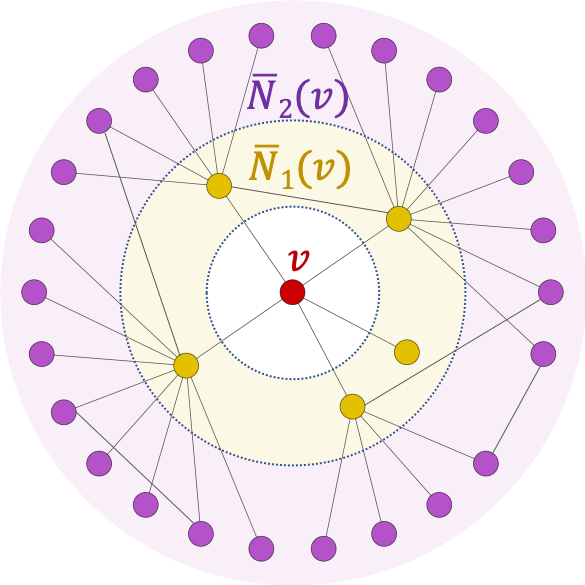
\includegraphics[width=0.25\textwidth]{submissions/Jiong2023/FIG/neighborhoods.png}
\caption{Neighborhoods.}
\label{fig:neighborhoods}
\end{wrapfigure}
In this section, we give the key notations and definitions that we use throughout our paper. 
Let $\graph=(\vertexSet,\edgeSet)$ be an undirected, unweighted graph with node set $\vertexSet$ and edge set $\edgeSet$. 
We denote a general neighborhood centered around $v$ as $N(v)$ ($\graph$ may have self-loops), the corresponding neighborhood that does \textit{not} include the ego (node $v$) as $\neighNoSelfLoop(v)$, and the general neighbors of node $v$ at exactly $i$ hops/steps away (minimum distance) as $\bar{N}_i(v)$. For example, as shown in Fig.~\ref{fig:neighborhoods}, $\bar{N}_1(v) = \{u: (u,v) \in \edgeSet \}$ are the immediate neighbors of $v$.
We represent the graph by 
its adjacency matrix $\matA \in \{0,1\}^{n\times n}$ 
and its node feature matrix $\matX \in \mathbb{R}^{n \times F}$, where 
the vector $\jV{x}_v$ corresponds to the \textit{ego-feature} of node $v$, 
and $\{\jV{x}_u: u \in \neighNoSelfLoop(v)\}$ to its \textit{neighbor-features}. 
We further represent the degree of a node $v$ by $d_v$, which denotes the number of neighbors in its immediate neighborhood $\bar{N}_1(v)$.

We further assume a class label vector $\vecy$, which for each node $v$ contains a unique class label $y_v \in \setY$, and the one-hot encoding $\mathrm{onehot}(y_v)$ forms the row vectors of label encoding matrix $\mathbf{Y} \in \{0,1\}^{n \times |\setY|}$. We further define $\vertexSet_i$ as the set of nodes $v \in \vertexSet$ with label $y_v = i$.
The goal of semi-supervised node classification is to learn a mapping $\ell: \vertexSet \rightarrow \setY$, given a set of labeled nodes $\setT = \{(v_1,y_1), (v_2, y_2), ...\}$ as training data.  


\paragraph{Graph Neural Networks (GNNs).} 
\label{sec:2-gnn}
From a probabilistic perspective, most GNN models assume the following local Markov property on node features: 
for each node $v \in \vertexSet$, there exists a neighborhood $N(v)$ such that
$y_v$ only depends on the ego-feature $\jV{x}_v$ and neighbor-features $\{\jV{x}_u: u \in N(v)\}$. 
Most models derive the class label $y_v$ via the following representation learning approach: {\small 
\begin{equation}
    \jV{r}^{(k)}_v = f\left(\jV{r}^{(k-1)}_v, \{\jV{r}^{(k-1)}_u: u \in N(v)\}\right),     \; \jV{r}^{(0)}_v = \jV{x}_v, \; \text{and} \;  y_v = \arg \max \{\mathrm{softmax}(\jV{r}^{(K)}_v)\matW\},
    \label{eq:gnn}
\end{equation}
}
where the embedding function $f$ is applied repeatedly in $K$ total rounds, 
node $v$'s representation (or hidden state vector) at round $k$, {\small $\jV{r}^{(k)}_v$}, is learned from its ego- and neighbor-representations in the previous round, and a softmax classifier with {learnable weight matrix} $\matW$ is applied to the final representation of $v$.
Most existing models differ in their definitions of neighborhoods $N(v)$ and embedding function $f$. 
A typical definition of neighborhood is $N_1(v)$---i.e., the 1-hop neighbors of $v$. 
As for $f$, in graph convolutional networks (GCN)~\cite{kipf2016semi} each node repeatedly averages its own features and those of its neighbors to update its own feature representation.  Using an attention mechanism, GAT~\cite{velickovic2018graph} models the influence of different neighbors more precisely as a weighted average of the ego- and neighbor-features. GraphSAGE~\cite{hamilton2017inductive} generalizes the aggregation beyond averaging, and models the ego-features distinctly from the neighbor-features in its subsampled neighborhood.


\paragraph{Homophily and heterophily.} 
\label{sec:homophily}

\begin{wrapfigure}{r}{0.33\textwidth}
    \vspace{-0.4cm}
    \centering
    \adjincludegraphics[width=0.3\textwidth, trim={0 0 0 {0.13\height}}, clip]{submissions/Jiong2023/FIG/example-graph.pdf}
    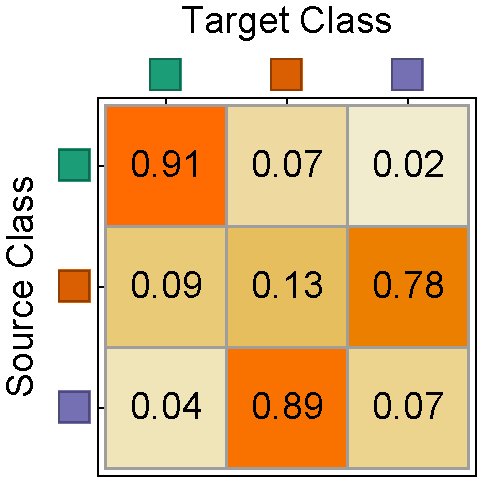
\includegraphics[width=0.2\textwidth]{submissions/Jiong2023/FIG/example-graph-comp.pdf}
    \caption{An example graph (top) and its empirical class compatibility matrix $\matH$ (bottom). It demonstrates mixed \emph{homophily} and \emph{heterophily}, with node colors represent class labels: nodes in green show strong homophily, while nodes in orange and purple show strong heterophily.}
    \label{fig:mixed-heterophily-example}
    \vspace{-0.9cm}
\end{wrapfigure}
In this work, we focus on heterophily in class labels. We first define the edge homophily ratio $h$ as a measure of the graph homophily level, and use it to define graphs with strong homophily/heterophily: 
\begin{definition}[Edge Homophily Ratio~\cite{MixHop,zhu2020beyond}]
The edge homophily ratio $h = \tfrac{|\{(u,v): (u,v) \in \edgeSet \wedge y_u = y_v\}|}{|\edgeSet|}$ is the fraction of edges in a graph which connect nodes that have the same class label (i.e., intra-class edges). 
\label{dfn:homophily-ratio}
\end{definition}
\begin{definition}\label{dfn:heterophily-nets}
Graphs with strong homophily have high edge homophily ratio $h  \rightarrow 1$, while graphs with strong heterophily (i.e., low/weak homophily) have small edge homophily ratio $h \rightarrow 0$. 
\end{definition}

The edge homophily ratio in Dfn.~\ref{dfn:homophily-ratio} gives an \textit{overall trend} for all the edges in the graph. The actual level of homophily may vary within different pairs of node classes, i.e., there is different tendency of connection between each pair of classes. 
For instance, in an online purchasing network~\cite{netprobe07} with three classes---fraudsters, accomplices, and honest users---, fraudsters connect with higher probability to accomplices and honest users. 
Moreover, within the same network, it is possible that some classes exhibit homophily, while others exhibit heterophily; we give an example in Figure~\ref{fig:mixed-heterophily-example}.
To capture the tendency of connection between each pair of classes, we define the empirical \textit{class compatibility matrix} $\matH$ as follows: %

\begin{definition}[Empirical Class Compatibility Matrix~\cite{zhu2020beyond,zhu2021graph}]
\label{dfn:compatibility-matrix-empirical}
The empirical class compatibility matrix $\matH$ has entries $[\matH]_{i,j}$ that capture the fraction of edges from a node in class $i$ to a node in class $j$: 
\begin{equation*}
    [\matH]_{i,j} = \frac{|\{(u,v): (u,v) \in \edgeSet \wedge y_u = i \wedge y_v = j\}|}{|\{(u,v): (u,v) \in \edgeSet \wedge y_u = i\}|}
\end{equation*}
\end{definition}
By definition, the class compatibility matrix is a stochastic matrix, with each row summing up to 1. 


\paragraph{Heterophily $\neq$ Heterogeneity.} 
We remark that heterophily, which we study in this work, is a distinct network concept from heterogeneity. 
Formally, a network is heterogeneous~\cite{SunH12} if it has at least two types of nodes and different relationships between them, and homogeneous if it has a single type of nodes (e.g., users) and a single type of edges (e.g., friendship). The type of nodes in heterogeneous graphs does \textit{not} necessarily match the class labels $y_v$, therefore both homogeneous and heterogeneous networks may have different levels of homophily. 














\section{Progress for Addressing Heterophily in GNNs}

In this section, we first present a concise overview of effective design strategies proposed to enhance GNN performance under heterophily (\S\ref{sec:progress-designs}), and then discuss the implications of these designs for other GNN research in robustness, fairness, and reducing oversmoothing (\S\ref{sec:progress-connections}).
\subsection{Effective Designs for Graph Neural Networks on Heterophilous Graphs}
\label{sec:progress-designs}

We present an overview of the effective design strategies that have been recently proposed to enhance GNN performance on heterophilous graphs. We initiate our discussion with widely adopted designs (D1-D4) in GNN architectures for heterophily, three of which were initially explored in \cite{zhu2020beyond}. Subsequently, we examine two emerging designs (D5-D6) introduced by \citet{yan2022two}, which offer a novel unified approach to address two significant challenges faced by GNNs: oversmoothing and heterophily. Our primary focus in this section is to discuss the design principles and their underlying intuition for improving learning under heterophily without delving into specific models; we direct interested readers to a comprehensive survey by \citet{zheng2022graph} for more details about particular models.





\subsubsection{Ego- and Neighbor-embedding Separation}
\citet{zhu2020beyond} identified three designs for improving the performance of GNNs on heterophilous graphs and provided theoretical justifications.
At a high level, the first design entails encoding each ego-embedding (i.e., a node's embedding) \textit{separately} from the aggregated embeddings of its neighbors, since they are likely to be dissimilar in heterophily settings. Formally, the representation (or hidden state vector) learned for each node $v$ at GNN layer with depth $k$ is given as:
\begin{equation}
        \jV{r}^{(k)}_v = \texttt{{COMBINE}}\left(\jV{r}^{(k-1)}_v, \; \texttt{AGGR}(\{\jV{r}^{(k-1)}_u: u \in {\neighNoSelfLoop(v)}\})\right),
    \label{eq:design1}
\end{equation}
the neighborhood $\neighNoSelfLoop(v)$ does \textit{not} include $v$ (no self-loops), the \texttt{AGGR} function aggregates representations \textit{only} from the neighbors (in some way---e.g., average), and \texttt{AGGR} and \texttt{COMBINE} may be followed by a non-linear transformation.
For heterophily, after aggregating the neighbors' representations, the definition of \texttt{COMBINE} (akin to `skip connection' between layers) is critical: the ego-embedding and the aggregated neighbor-embedding should be processed by different sets of weight matrices under \texttt{COMBINE}.
A simple way to combine the ego- and the aggregated neighbor-embeddings without `mixing' them is with concatenation {as in GraphSAGE~\cite{hamilton2017inductive}}---rather than averaging \textit{all} of them as in the GCN model by~\citet{kipf2016semi}. Intuitively, \cite{zhu2020beyond} argues that choosing a \texttt{COMBINE} function that separates the representations of each node $v$ and its neighbors $\neighNoSelfLoop(v)$ allows for more expressiveness, where the skipped or non-aggregated representations can evolve separately over multiple rounds of propagation without becoming prohibitively similar to representations aggregated from neighbors.

While this design was first discussed in \cite{zhu2020beyond} as the most critical design in the context of improving GNN performance under heterophily, 
it had already been proposed and adopted in prior GNN models such as GraphSAGE~\cite{hamilton2017inductive}, without addressing the problem of heterophily. GCN-Cheby~\cite{defferrard2016convolutional} and MixHop~\cite{MixHop} %
also feature a variant of this design, with the \texttt{AGGR} function operating on $N(v)$ (with self-loops) instead of $\neighNoSelfLoop(v)$ (no self-loops), while still featuring a separate channel for the ego-embedding.
Following \method proposed in \cite{zhu2020beyond}, this design has gained wide adaptation for GNNs designed with heterophilous graphs in mind, such as CPGNN~\cite{zhu2021graph}, GPR-GNN~\cite{chien2021adaptive}, FAGCN~\cite{zhang2021beyond}, FSGNN~\cite{zhang2021improving}, JacobiConv~\cite{li2021jacobi}, GGCN~\cite{yan2022two}, GBK-GNN~\cite{du2022gbk}, ACM~\cite{luan2022revisiting}, and OrderedGNN~\cite{song2023ordered}.
More recently, \citet{platonov2023critical} conducted benchmark experiments on additional heterophilous datasets and showed that GNNs featuring this design, including GAT~\cite{velickovic2018graph} and UniMP~\cite{shi2021masked} modified to include this design, achieve the best results in nearly all cases, which further validates the importance of the ego \& neighbor embedding separation.

\subsubsection{Higher-order Neighborhoods} The second design in \cite{zhu2020beyond} involves explicitly aggregating information from higher-order neighborhoods in each GNN layer, beyond the immediate neighbors of each node: 
\begin{equation}
    \jV{r}^{(k)}_v = \texttt{COMBINE}\left(\jV{r}^{(k-1)}_v, \; \texttt{AGGR}_1(\{\jV{r}^{(k-1)}_u: u \in {\bar{N}_1(v)}\}), \; \texttt{AGGR}_2(\{\jV{r}^{(k-1)}_u: u \in {\bar{N}_2(v)}\}), \ldots \right),
\end{equation}

where $\bar{N}_i(v)$ denotes the neighbors of $v$ at \textit{exactly} 
$i$ hops away, and the $\texttt{AGGR}_i$ functions applied to different neighborhoods can be the same or different. This design---first employed in GCN-Cheby~\cite{defferrard2016convolutional} and MixHop~\cite{MixHop}---augments the \textit{implicit} aggregation over higher-order neighborhoods that most GNN models achieve through multiple layers of first-order propagation based on variants of Eq.~\eqref{eq:design1}. 
\citet{zhu2020beyond} attribute the effectiveness of this design to observations that even though the immediate neighborhoods may be heterophilous, the higher-order neighborhoods may show homophily in certain datasets (e.g., binary attribute prediction on 2-partite graphs~\cite{altenburger2018monophily,chin2019decoupled}) and thus provide more relevant context to GNNs. 

Early implementations of this design, such as GCN-Cheby~\cite{defferrard2016convolutional} and MixHop~\cite{MixHop}, extract embeddings from higher-order neighborhoods $\bar{N}_i(v)$ within each layer by employing ``Delta Operators''~\cite{MixHop}. These operators differentiate the aggregated embeddings in different orders of the (normalized) adjacency matrices $\matA^{i}$ and $\matA^{i-1}$ for improved computational efficiency. In contrast, \method\cite{zhu2020beyond}, UGCN~\cite{jin2021universal}, TDGNN~\cite{wang2021tree}, and OrderedGNN~\cite{song2023ordered} precisely compute the $i$-hop neighborhoods $\bar{N}_i(v)$ for each node $v$ before applying the $\texttt{AGGR}_i$ functions to prevent mixing nodes from different hops. Notably, the recent approach by \citet{song2023ordered} achieves state-of-the-art classification accuracy on heterophilous datasets by modeling message passing within higher-order neighborhoods using a rooted-tree hierarchy, and aligning segments of variable length in the resulting node embeddings with specific neighborhood orders.

\subsubsection{Combination of Intermediate Representations} The third design proposed in \cite{zhu2020beyond} combines the intermediate representations of each node at the final layer: 
\begin{equation}
    \jV{r}^{(\text{final})}_v = \texttt{COMBINE}\left({\jV{r}^{(1)}_v, \jV{r}^{(2)}_v, \ldots}, \jV{r}^{(K)}_v \right).
\end{equation}
This approach explicitly captures both local and global information using \texttt{COMBINE} functions that process each representation individually, such as concatenation or LSTM-attention~\cite{XuLTSKJ18-jkn}. This design was initially introduced in jumping knowledge networks~\cite{XuLTSKJ18-jkn} and demonstrated to enhance the representation power of GCNs under \textit{homophily}. Intuitively, each GNN layer gathers information with varying degrees of locality—earlier layers focus on local information, while later layers increasingly capture global information (implicitly, through propagation). Similar to D2 (which models explicit neighborhoods), this design models the distribution of neighbor representations in low-homophily networks more accurately.
It also allows the class prediction to leverage different neighborhood ranges in different networks, adapting to their structural properties. 

The application of this design is often linked to graph spectral theory: \citet{zhu2020beyond}  provided a theoretical justification for this design from the perspective of graph spectral filtering. Building upon this foundation, GPR-GNN~\cite{chien2021adaptive}, FAGCN~\cite{bo2021beyond}, and ACM~\cite{luan2022revisiting} further enhance GNN performance under heterophily by developing additional graph filters and mixture mechanisms to utilize embeddings generated with varying frequency components at the final layer, in conjunction with this design.

\subsubsection{Similarity-based Attention and Neighbor Discovery}
The designs identified in \cite{zhu2020beyond} focus on boosting the effectiveness of message passing on heterophilous graphs without modifying the underlying structure. An alternative approach, however, is to go beyond the original graph adjacency and discover additional connections between the nodes in the graph, based on the similarity their original or latent features (e.g., structural embeddings), which replace or augment the original heterophilous structure of the graph in the message passing. 
Specifically, UGCN~\cite{jin2021universal}, SimP-GCN~\cite{jin2021node}, NL-GNN~\cite{liu2021non}, HOG-GCN~\cite{wang2022powerful} and GPNN~\cite{yang2022graph} update the message-passing graph for GNNs by removing or downweighting the heterophilous edges in the original graph (i.e., edges that connect nodes with dissimilar features or structural embeddings), while introducing newly discovered connections that exhibit strong homophily. 
On the other hand, Geom-GCN~\cite{Pei2020Geom-GCN} and WRGNN~\cite{suresh2021breaking} leverage for each node both its original graph neighborhood and the derived ``structural neighborhood'' based on proximity of structural node embeddings in order to augment the message passing and aggregation process. 

\subsubsection{Signed Messages \& Gated Kernel}
In most GNN models~\cite{kipf2016semi,velickovic2018graph}, messages are positively aggregated from neighbors and transformed using a single kernel or weight matrix. However, in heterophilous graphs, this may degrade GNN performance when messages from neighbors of different classes are mixed~\cite{zhu2020beyond,yan2022two}. Although attention-based GNNs, such as GAT~\cite{velickovic2018graph}, can theoretically reduce aggregation weights on heterophilous edges, they may still accumulate noise in the generated embeddings in practice.

An intuitive solution to address this issue is to learn signed messages (e.g., GGCN~\cite{yan2022two} and GReTo~\cite{zhou2023greto}) or gated kernels (e.g., GBK~\cite{du2022gbk}) that separate message passing between homophilous intra-class and heterophilous inter-class edges. \citet{yan2022two} suggested that ideally, messages from neighbors of a different class should be multiplied by a negative sign (``negative messages''), while messages from neighbors of the same class should remain unchanged. However, ground truth node labels are inaccessible in real scenarios, and any approximated sign function may introduce errors. To identify conditions when signed messages can enhance node classification performance, \cite{yan2022two} introduced the concept of ``error rate'' that quantifies the portion of non-ideal messages and analyzed node classification performance under various error rates and homophily levels.
The benefits of using signed messages can also be interpreted from the perspective of graph spectrum: signed messages allow negative mixture of certain frequency components~\cite{zhang2021beyond, chien2021adaptive}, helping models better capture high-frequency components in node features. This is especially beneficial for learning on heterophilous graphs as they contain abundant high-frequency components in their node features, unlike homophilous graphs~\cite{zhu2020beyond}.

From the perspective of practical model design, GGCN~\cite{yan2022two} and GReTo~\cite{zhou2023greto} used proximity between node features to approximate the sign function. As an alternative to signed messages, \citet{du2022gbk} proposed a gated bi-kernel design that applies separately to the message passing of homophilous and heterophilous edges, and adopted a learnable gate function to distinguish between the two types of edges based on the node features.

\subsubsection{Degree Corrections}
Zhu et al.~\cite{zhu2020beyond} first noted that the performance divide between low- and high-degree nodes is exacerbated on heterophilous graphs (c.f. Figure~\ref{fig:h2gcn-degree-acc}). 
Later, \citet{yan2022two} provided a thorough theoretical and empirical analysis of how the interplay of degrees and homophily levels affects the node classification accuracy. Specifically, two node-level properties were defined: relative degree ${\bar{\theta}_u}$, which evaluates the degree of a node compared to its neighbors' degrees; and node-level homophily $h_u$, which captures the tendency of a node to have the same class as its neighbors. 
Formally, the relative degree of a node $u$ is defined as ${\bar{\theta}_u}\equiv\mathbb{E}_{\mathbf{A}|d_u}(\frac{1}{d_u} \sum_{v \in N_1(u)} \theta_{uv}|d_u), \text{where } \theta_{uv}\equiv\sqrt{\frac{d_u + 1}{d_v + 1}}$; and the node-level homophily $h_u$ is defined as $h_u \equiv \mathbb{P}(y_u=y_v|v \in N_1(u)).$ 
The authors discovered that nodes with higher relative degrees outperform the nodes with lower ones under certain conditions of node features when
the design of signed messages (D5) is employed.
To improve the performance of nodes with lower relative degrees, they proposed a degree correction strategy which learns to virtually increase the relative degree of the nodes via structure-based edge attention weights $\tau_{uv}^l = \texttt{softplus}\left (\lambda_0^l\left (\tfrac{1}{\theta_{uv}}-1\right )+\lambda_1^l\right )$, where $\lambda_0^l$ and $\lambda_1^l$ are the learnable parameters at the $l$-th GNN layer. If $\theta_{uv}$ is small, a large $\tau_{uv}^l$ is learned, which compensates for the current relative degree.





\subsection{Heterophily and Other Objectives of GNN Research}
\label{sec:progress-connections}

Numerous studies have demonstrated that tackling the limitations of GNNs under heterophily not only enhances their performance on heterophilous datasets, but also improves their properties in other aspects of GNN research. In this section, we provide an overview of the connections that have been investigated between heterophily and adversarial robustness, algorithmic fairness, and oversmoothing, all of which are also important for deployment. 

\paragraph{Heterophily \& Robustness.}
Recent works have shown that GNNs have a high sensitivity to adversarial attacks~\cite{zugner2018adversarial,dai2018adversarial,xu2019topology,wu2019adversarial,li2020adversarial,ma2020towards}. While most previous works have focused on naturally-occurring heterophily, heterophilous interactions may also be introduced as adversarial noise: 
as many GNNs exploit homophilous correlations, they can be sensitive to changes that render the data more heterophilous. 
This relation between adversarial structural attacks and the change of homophily level was first suggested though empirical analyses on homophilous graphs~\cite{wu2019adversarial,jin2020adversarial}, and was later formalized by \citet{zhu2022heterophily} with theoretical and additional empirical analyses. Specifically, \citet{zhu2022heterophily} showed that on homophilous graphs, effective structural attacks lead to increased heterophily, while, on heterophilous graphs, they alter the homophily level contingent on node degrees: 
for low-degree nodes, attacks increasing the heterophily are still effective, but 
for high-degree nodes, attacks \emph{decreasing} the heterophily will be effective. 
By leveraging these relations, the authors further demonstrated that some key architectural designs for effectively handling heterophily---separate aggregators 
for ego- and neighbor-embeddings (D1) and Combination of Intermediate Representations (D3)---also improve the robustness of GNNs against attacks. 
Following these relations, a follow-up work proposed a defense framework called CHAGNN that improves the robustness of GNNs against Graph Injection Attacks (GIA) by iteratively pruning the heterophilous edges in the graph and retraining the GNN model~\cite{zhu2023resisting}.

\paragraph{Heterophily \& Fairness.}
Algorithmic fairness is a critical aspect of machine learning that ensures a model does not disproportionately underperform for certain input classes. In the context of link prediction in networks, fairness is desirable to prevent the prediction accuracy from being influenced by sensitive node attributes, such as race or religion in a social network context. To promote fairness in Graph Neural Networks (GNNs), previous research has suggested learning a fair reweighting or rewiring of the graph structure alongside the parameters of the GNN~\cite{li2021dyadic,spinelli2021fairdrop}. Theoretical analysis has shown that the effectiveness of these approaches depends on the weights of the intergroup edges (essentially, heterophilous edges according to sensitive attribute), along with the group sizes and other structural attributes of the graph.
For node classification, the global homophily ratio of a graph has revealed to be crucial in providing bounds for group fairness concerning a sensitive attribute~\cite{wang2022improving}. Other research has examined GNN fairness with respect to local homophily ratios within individual node neighborhoods~\cite{loveland2022graph}, revealing that variations in local homophily can impact model fairness, and that GNN designs for heterophily can empirically enhance group fairness.

\paragraph{Heterophily \& Oversmoothing.}
The oversmoothing problem relates to the degenerated performance of GNNs with an increasing number of layers~\cite{li2018deeper}. 
Though both the heterophily and oversmoothing problems are associated to the unsatisfactory performance of GNNs, they do not appear to be related at a first glance. However, evidence from both empirical~\cite{chen2020simple, chien2021adaptive} and theoretical analysis~\cite{yan2022two, bodnar2022neural} has found that the two problems may share the same root causes and may be addressed with the same approaches.
\citet{chen2020simple} addressed the oversmoothing problem via initial residual and identity mapping, but their designs were found empirically to help improve the node classification performance on heterophilous graphs. 
Vice versa, \citet{chien2021adaptive} addressed the heterophily problem via generalized PageRank, but they showed that their designs are also effective for addressing the oversmoothing problem. 
\citet{yan2022two} are the first to explicitly analyze the relationship between the two problems. They found that the two problems can be jointly explained by analyzing the changes in the node representations over the layers, and proposed two designs, namely signed messages (D5) and degree corrections (D6), to address the two problems jointly.
Later, \citet{bodnar2022neural} used cellular sheaves theory to explain the two problems jointly. They found that the underlying geometry of the graph is related to the performance of GNNs in heterophilous settings and their oversmoothing behavior, and many GNNs implicitly assume a graph with a trivial underlying sheaf. These observations and analyses have shown promising results in addressing the two problems jointly, which is an interesting direction to explore further.
\section{Revisiting When is Heterophily Challenging for GNNs}
\label{sec:complexity}

While many works have focused on designing new GNN models with improved performance under heterophily, few of them have probed whether heterophily persistently presents challenges for GNNs. Some of these works have found that GNNs without the aforementioned heterophilous designs (e.g., SGC~\cite{wu2019simplifying}, GCN~\cite{kipf2016semi}, GAT~\cite{velickovic2018graph}) can exhibit better or equivalent performance to GNNs possessing such designs \emph{on certain datasets}~\cite{ma2021homophily,luan2022revisiting}.
In this section, we first summarize the main findings of these works, 
and show that the complexity of heterophily can be measured based on the distinguishability of the Neighborhood Label Distributions (NLDs).\footnote{In parallel with these studies, \citet{yan2022two} conducted a theoretical analysis of performance degradation in heterophilous networks under the ``non-swapping'' condition. This condition emerges when the neighboring representations for each node are \emph{insufficient} to cause the interchange of node representations from two distinct classes across their separation plane in the latent space. Conversely, the case of ``easy heterophily''~\cite{ma2021homophily,luan2022revisiting} that we address in this section corresponds to the ``swapping'' condition as articulated in \cite{yan2022two}.}
We then highlight two key factors, low-degree nodes and complex compatibility matrices, which deteriorate the distinguishability of the neighborhood label distributions when coupled with heterophily, thus making heterophily a unique challenge for GNNs in most cases. 


\subsection{Improved Measures for Complexity of Heterophily}
\label{sec:complexity-measurements}

While many works measure the level of homophily/heterophily by the ratio of edges that connect nodes with the same class label (e.g., edge homophily in Dfn.~\ref{dfn:homophily-ratio}, node homophily~\cite{Pei2020Geom-GCN}, or class homophily~\cite{lim2021large}), recent works have shown that graphs with high heterophily are not always challenging for GNNs without heterophilous designs. 
Through independent analyses, \citet{ma2021homophily} and \citet{luan2022revisiting} arrive at the conclusion that the complexity of heterophily is closely related to the distinguishability of the neighborhood label distributions, which we define next. 

\begin{definition}[Neighborhood Label Distribution (NLD)]
Given $\mathbf{Y}$ as the label encoding matrix defined in \S\ref{sec:preliminaries} for nodes $\vertexSet$ in graph $\graph$, the neighborhood label distribution of node $v$ is defined as
$\mathbf{D}(v) = \tfrac{1}{|N_1(v)|} \sum_{u \in N_1(v)} \mathbf{Y}_u$, where $\mathbf{Y}_u = \mathrm{onehot}(y_u)$ is the $v$-th row of the label encoding matrix $\mathbf{Y}$.
\end{definition}

We now rephrase the two metrics proposed by \citet{ma2021homophily} and \citet{luan2022revisiting} with the above definition, both of which measure the complexity of heterophily by quantifying the distinguishability of $\mathbf{D}(v)$.

\begin{definition}[Class Neighborhood Similarity (CNS)~\cite{ma2021homophily}] %
The class neighborhood similarity between classes $i, j \in \setY$ is defined as the average cosine similarity between the NLDs $\mathbf{D}(v), \mathbf{D}(u)$ of nodes $v, u$ in class $i$ and $j$, respectively, i.e.,
\begin{equation}
    \label{eq:complexity-CNS}
    S(i, j) = \frac{1}{|\vertexSet_i||\vertexSet_j|}\sum_{v \in \vertexSet_i} \sum_{u \in \vertexSet_j} \mathrm{sim}_{\mathrm{cos}}(\mathbf{D}(v), \mathbf{D}(u)),
\end{equation}
where $\vertexSet_i$ and $\vertexSet_j$ are the sets of nodes with class label $i$ and $j$, and $\mathrm{sim}_{\mathrm{cos}}(\cdot)$ is the function of cosine similarity. 
We refer to the case of $i=j$ as \emph{intra-class neighborhood similarity (intra-CNS)} and the case of $i \neq j$ as \emph{inter-class neighborhood similarity (inter-CNS)}.
\end{definition}

\begin{definition}[Graph Aggregation Homophily~\cite{luan2022revisiting}]
Define the average similarity score of a node $v \in \vertexSet$ to nodes $\vertexSet_i$ with class label $i \in \setY$ as
$g(v, i) = \mathrm{mean}\left(\left\{\mathrm{sim}(\mathbf{D}(v), \mathbf{D}(u)) : v, u \in \vertexSet, y_u = i \right\}\right)$, where $\mathrm{sim}$ is a function (e.g., dot product) that measures the similarity between two neighborhood label distributions.
The graph aggregation homophily is then defined as the ratio of nodes $v \in \vertexSet$ where the neighborhood label distribution $\mathbf{D}(v)$ is more similar for nodes in the same class than for nodes in any other class, i.e.,

\begin{equation}
    \label{eq:complexity-gah}
    h_{\mathrm{agg}} = \frac{1}{|\vertexSet|} 
    \left|\left\{ v \in \vertexSet :
    g(v, y_v)
    \geq 
    \max_{j \neq y_v \in \setY}  g(v, j)
    \right\}\right|.
\end{equation}
\end{definition}
We note that while $h_{\mathrm{agg}}$ measures the \textit{proportion} of nodes with NLD exhibiting \emph{greater} similarity (regardless of the extent) to nodes within the same class compared to nodes from different classes, it does not quantify the \textit{degree of similarity} between NLDs of nodes within the same class or across different classes, which is captured by the CNS metric. Consequently, as we show in our empirical analysis in \S\ref{sec:complexity-experiments}, CNS provides a more comprehensive and accurate assessment of the complexity of heterophily on synthetic datasets, and thus we focus on CNS in our empirical analysis below.


\subsection{Factors Determining the Complexity of Heterophily}
It has been shown that it is possible to have graphs with high level of heterophily but low complexity for GNNs as measured by CNS or aggregation homophily~\cite{ma2021homophily,luan2022revisiting}: when nodes in the same class have strong similarity with respect to neighborhood label distributions, and nodes from different classes have weak or no similarity, GCN models are able to perform well due to the high distinguishability of the neighborhood label distributions, even when the graphs are heterophilous.
These are important findings, but this type of analysis does not provide a complete picture of the complexity of heterophily for GNNs, as the high distinguishability of the class label distributions under heterophily is largely dependent on key graph properties, such as degree distributions and the compatibility matrices that drive the generation of the graph. In this section, we provide a detailed analysis of the above two factors that determine how challenging the data heterophily is for GNNs. 

\subsubsection{Motivating Example: Differences in Synthetic Datasets} 
\label{sec:complexity-motivating-example}

Prior research exploring the impact of heterophily on GNN performance frequently incorporates experiments on synthetic datasets with controlled homophily/heterophily levels~\cite{MixHop,zhu2020beyond,ma2021homophily,luan2022revisiting}. 
In line with this research, in this section we provide a motivating example based on synthetic data that showcases the role of the two factors---namely, degree distribution and compatibility matrices---in characterizing how challenging heterophily is for GNN models.
We analyze the seemingly contradictory observations arising from the results on two distinct synthetic datasets based on the \texttt{Cora} dataset: \texttt{syn-cora}~\cite{zhu2020beyond} and \texttt{necessity-cora}~\cite{ma2021homophily}.

Before diving into the analysis of the factors that affect the complexity of heterophily, we first provide a brief overview on the setup and key results on the two synthetic datasets~\cite{zhu2020beyond,ma2021homophily}.

\paragraph{Data Generation: \texttt{syn-cora} vs.~\texttt{necessity-cora}.} 
While both synthetic datasets are generated based on \texttt{Cora}, their generation processes are largely different. 
The \texttt{syn-cora} dataset~\cite{zhu2020beyond,zhu2021graph} follows a modified preferential attachment process. In this process, the probability of a new node $u$ with class label $c$ to attach to existing node $v$ with class label $c'$ is proportional to: 
(1) the ratio $\mathcal{D}_{c,c'}$ specified in the \emph{underlying} compatibility matrix $\mathcal{D}$, which determines the homophily level in the resulting graph, as empirically measured by the edge homophily ratio $h$ (Dfn.~\ref{dfn:homophily-ratio}) and the compatibility matrix $\mathbf{H}$ (Dfn.~\ref{dfn:compatibility-matrix-empirical}),
and (2) the degree $d_v$ of the existing node $v$.
This process results in a power-law degree distribution in the generated graph. 
On the other hand, \texttt{necessity-cora}~\cite{ma2021homophily} varies the level of homophily by adding heterophilous (cross-label) edges on top of the existing (homophilous) edges in \texttt{Cora}. 
To control the randomness of the added heterophilous edges, \texttt{necessity-cora} adds: 
(1) non-random heterophilous edges based on an \emph{underlying} compatibility matrix $\mathcal{D}$, and 
(2) random edges that do not follow the underlying compatibility matrix $\mathcal{D}$, but are controlled by a noise parameter $\gamma$. 

\begin{figure}
    \centering
    \begin{subfigure}[t]{0.453\textwidth}
        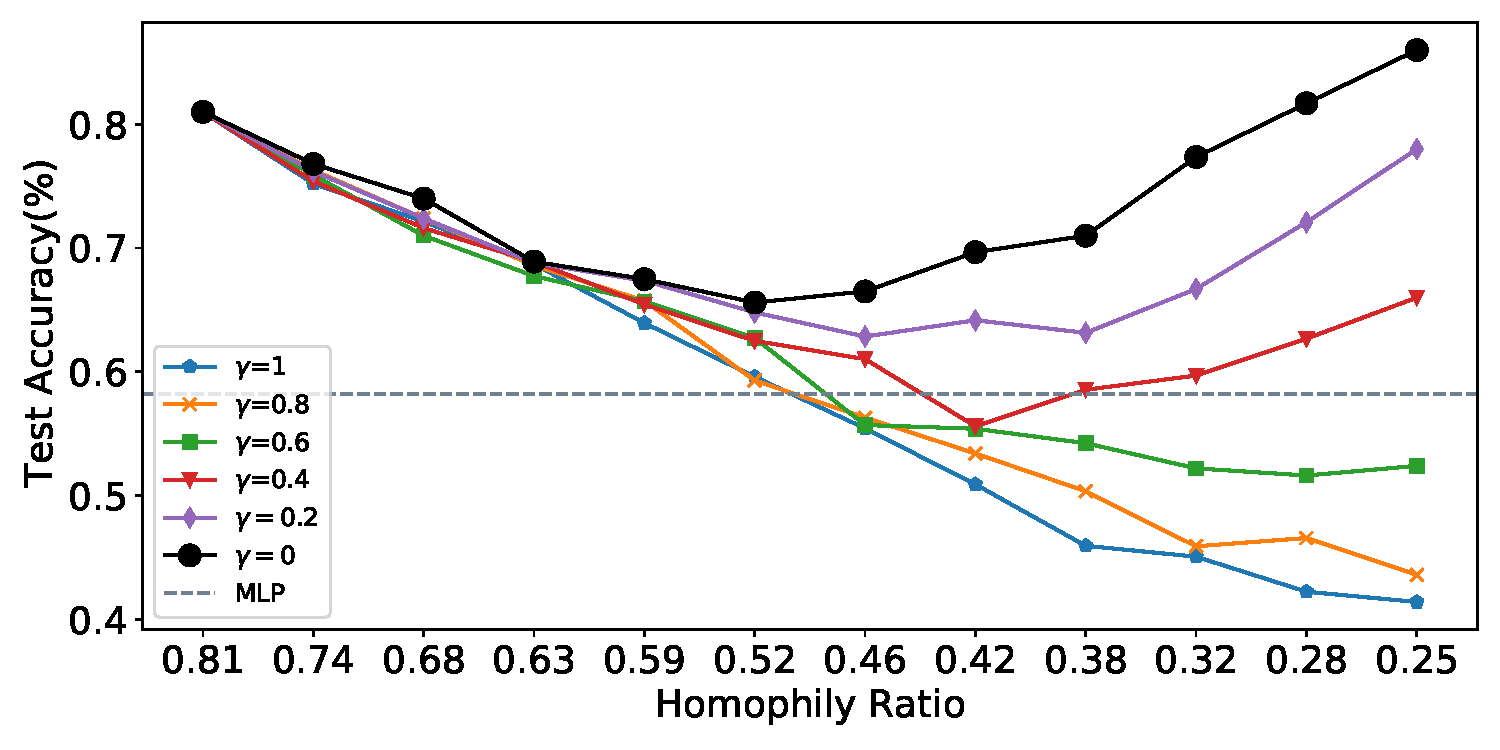
\includegraphics[width=\textwidth]{submissions/Jiong2023/FIG/revisiting-heterophily-GNNs/cora_homo.pdf}
        \caption{Accuracy on \texttt{necessity-cora} %
        under different noise levels $\gamma$. %
        Figure is reproduced from \cite{ma2021homophily}; shared with permission by the authors.}
        \label{fig:revisit-related-observations-necessity-cora}
    \end{subfigure}
    \hspace{0.05\textwidth}
    \begin{subfigure}[t]{0.44\textwidth}
        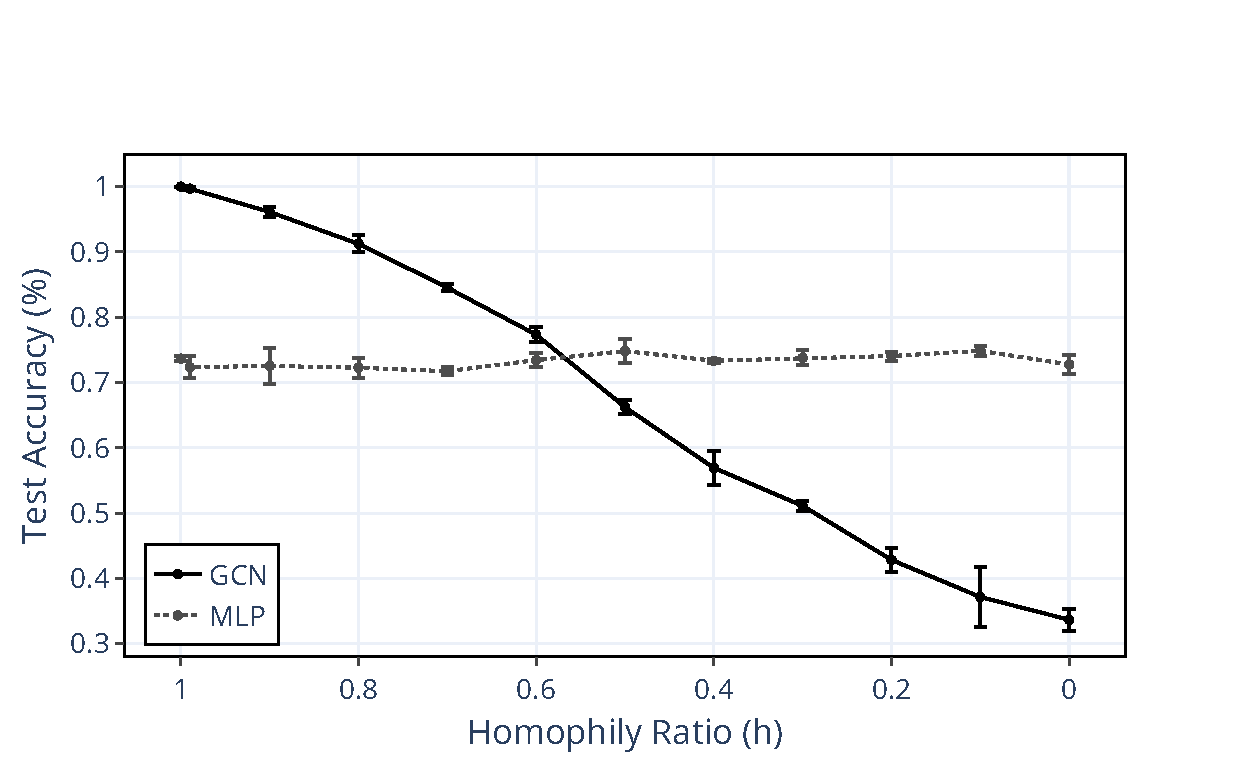
\includegraphics[width=\textwidth]{submissions/Jiong2023/FIG/revisiting-heterophily-GNNs/syn-cora-GCN-results.pdf}
        \caption{Accuracy on \texttt{syn-cora} for  GCN and MLP reported by \cite{zhu2020beyond}. Figure is adapted from \cite{zhu2020beyond}.}
        \label{fig:revisit-related-observations-syn-cora}
    \end{subfigure}
    \caption{Semi-supervised node classification accuracy of GCN and MLP observed in \cite{ma2021homophily} and \cite{zhu2020beyond} on \texttt{necessity-cora} and \texttt{syn-cora}, respectively, under increasing level of \emph{heterophily} (i.e., decrease of the edge homophily ratio $h$). 
    }
    \label{fig:revisit-related-observations}
\end{figure}

\paragraph{Observations: \texttt{syn-cora} vs.~\texttt{necessity-cora}.} 
When the level of heterophily is varied, 
largely different observations are reported on the two sets of synthetic graphs with respect to the GNN performance:
\cite{ma2021homophily} shows that on synthetic graphs with none or few \emph{randomly}-added heterophilous connections (i.e., with the noise parameter $\gamma$ close to 0),
the performance of GCNs can even increase as the level of heterophily in the graph gets stronger (i.e., when the edge homophily ratio $h$ decreases), as shown in Figure~\ref{fig:revisit-related-observations}(\subref{fig:revisit-related-observations-necessity-cora});
on the other hand, \cite{zhu2020beyond} shows that the performance of GCNs significantly decreases 
as the heterophily increases, which we show in Figure~\ref{fig:revisit-related-observations}(\subref{fig:revisit-related-observations-syn-cora}).
As our follow-up analysis below shows, these seemingly contradictory results are due to the different processes used to generate the synthetic graphs, which lead to very different graph properties (i.e., degree distribution, class compatibility matrix); these in turn affect the model performance.
We analyze the effects of the (F1) degree distribution in \S\ref{sec:complexity-factor-degree} and the (F2) compatibility matrix in \S\ref{sec:complexity-factor-compatibility}.

\subsubsection{Factor (F1): Degree Distributions \& Heterophily}
\label{sec:complexity-factor-degree}

In \S\ref{sec:complexity-measurements}, we revisit the findings from recent works~\cite{ma2021homophily,luan2022revisiting} that the complexity of heterophily for GNNs is largely determined by the distinguishability of the Neighborhood Label Distributions (NLDs) of nodes with different class labels. 
Under the generation process of \texttt{necessity-cora} with noise $\gamma=0$ (\S\ref{sec:complexity-motivating-example}), when classes are different $c \neq c'$ and the distributions $\mathcal{D}_{c}$ and $ \mathcal{D}_{c'} $ are distinguishable from each other, one would state that the GCN models can perform well to distinguish the nodes with class label $c$ from the nodes with class label $c'$ from the perspective of NLD distinguishability.



However, we argue that the aforementioned statement ignores the critical factor of degree for each node $v \in \mathcal{V}_c$ that impacts the quality of the samples of the distribution $\mathcal{D}_c$: when all the nodes have sufficiently large degrees, it is expected that $\mathcal{D}_c$ can be recovered well in the node neighborhoods due to sufficient samples of the distributions; however, when many low-degree nodes are present in the graph (which is the case for many real-world graphs, which usually follow power-law degree distributions), $\mathcal{D}_c$ may not be consistently recovered in the neighborhood of the low-degree nodes under heterophily due to the insufficiency of the samples. This affects the intra-class and inter-class similarity of the NLDs in heterophilous settings.


\paragraph{Empirical Analysis.} We can further explain how low-degree nodes affect the intra-class and inter-class distinguishability of the NLD for GCNs under heterophily with a simple empirical analysis: 
Suppose the neighborhood label distributions $\mathcal{D}_c$ and $\mathcal{D}_{c'}$ for two classes $c \neq c'$ are given in the red dashed boxes in Figure~\ref{fig:revisit-degree}.
Following the distributions $\mathcal{D}_c$ and $\mathcal{D}_{c'}$, we randomly generate the NLDs of 200 nodes with degree 2 for both classes $c$ and $c'$; then, we sample the labels of their 2 neighbors, and we visualize a random set of 5 of the 200 synthetic NLDs in Figure~\ref{fig:revisit-degree}(\subref*{fig:revisit-degree-low-heterophily-1})-(\subref*{fig:revisit-degree-low-heterophily-2}), for $\mathcal{D}_c$ and $\mathcal{D}_{c'}$, respectively.
We note that since GCN aggregators additionally consider a self-loop for each node, the NLD observed by GCN models should be considered with self-loops added to the graphs, even when $\mathcal{D}_c$ and $\mathcal{D}_{c'}$ dictate purely heterophilous connections. 
To visualize the contributions of self-loops in the NLDs, we show them in gray in Figure~\ref{fig:revisit-degree}.


\begin{figure}[tp]
    \centering
    \begin{subfigure}[b]{\textwidth}
       \caption*{\textbf{Case 1: Low-degree nodes \& heterophily}}
           \vspace{-0.6cm}
    \end{subfigure}
    \begin{subfigure}[b]{0.47\textwidth}
        \adjincludegraphics[width=\textwidth, trim={0 10.5cm {.5\width} 0}, clip]{submissions/Jiong2023/FIG/revisiting-heterophily-GNNs/dist-hete-low-degree.pdf}
        \caption{\emph{Heterophilous} distribution $\mathcal{D}_c$ of class $c$ (in red box) and 5 sampled NLDs for nodes with degree 2.}
        \label{fig:revisit-degree-low-heterophily-1}
    \end{subfigure}
    \hspace{0.04\textwidth}
    \begin{subfigure}[b]{0.47\textwidth}
        \adjincludegraphics[width=\textwidth, trim={{.5\width} 10.5cm 0 0}, clip]{submissions/Jiong2023/FIG/revisiting-heterophily-GNNs/dist-hete-low-degree.pdf}
        \caption{\emph{Heterophilous} distribution $\mathcal{D}_{c'}$ of another class $c'$ (in red box) and 5 sampled NLDs for nodes with degree 2.}
        \label{fig:revisit-degree-low-heterophily-2}
    \end{subfigure}
    \begin{subfigure}[b]{\textwidth}
       \caption*{\textbf{Case 2: High-degree nodes \& heterophily}}
           \vspace{-0.6cm}
    \end{subfigure}
    \begin{subfigure}[b]{0.47\textwidth}
        \adjincludegraphics[width=\textwidth, trim={0 10.5cm {.5\width} 0}, clip]{submissions/Jiong2023/FIG/revisiting-heterophily-GNNs/dist-hete-high-degree.pdf}
        \caption{\emph{Heterophilous} distribution $\mathcal{D}_c$ of class $c$ (in red box) and 5 sampled NLDs for nodes with degree 10.}
        \label{fig:revisit-degree-high-heterophily-1}
    \end{subfigure}
    \hspace{0.04\textwidth}
    \begin{subfigure}[b]{0.47\textwidth}
        \adjincludegraphics[width=\textwidth, trim={{.5\width} 10.5cm 0 0}, clip]{submissions/Jiong2023/FIG/revisiting-heterophily-GNNs/dist-hete-high-degree.pdf}
        \caption{\emph{Heterophilous} distribution $\mathcal{D}_{c'}$ of another class $c'$ (in red box) and 5 sampled NLDs for nodes with degree 10.}
        \label{fig:revisit-degree-high-heterophily-2}
    \end{subfigure}
    \begin{subfigure}[b]{\textwidth}
       \caption*{\textbf{Case 3: Low-degree nodes \& homophily}}
           \vspace{-0.6cm}
    \end{subfigure}
    \begin{subfigure}[b]{0.47\textwidth}
        \adjincludegraphics[width=\textwidth, trim={0 10.5cm {.5\width} 0}, clip]{submissions/Jiong2023/FIG/revisiting-heterophily-GNNs/dist-homo.pdf}
        \caption{\emph{Homophilous} distribution $\mathcal{D}_c$ of class $c$ (in red box) and 5 sampled NLDs for nodes with degree 2.}
        \label{fig:revisit-degree-low-homophily-1}
    \end{subfigure}
    \hspace{0.04\textwidth}
    \begin{subfigure}[b]{0.47\textwidth}
        \adjincludegraphics[width=\textwidth, trim={{.5\width} 10.5cm 0 0}, clip]{submissions/Jiong2023/FIG/revisiting-heterophily-GNNs/dist-homo.pdf}
        \caption{\emph{Homophilous} distribution $\mathcal{D}_{c'}$ of another class $c'$ (in red box) and 5 sampled NLDs for nodes with degree 2.}
        \label{fig:revisit-degree-low-homophily-2}
    \end{subfigure}
    \caption{{(Factor F1) Degree Distributions}: Per case, we sample 200 NLDs from distribution $\mathcal{D}_c$ (and $\mathcal{D}_{c'}$) for nodes with specific degrees, and visualize 5 sampled NLDs. The gray parts correspond to the contributions of self-loops in the NLDs aggregated by GCN. 
    \textbf{(\subref*{fig:revisit-degree-low-heterophily-1})-(\subref*{fig:revisit-degree-low-heterophily-2}) Case 1:} Low degrees reduce the distinguishability of NLDs: for all synthetic NLDs of $c$ and $c'$, inter-CNS is $S(c, c') = 0.79 \pm 0.17$, with even smaller standard deviation than intra-CNS $S(c, c) = S(c', c') = 0.79 \pm 0.24$.  
    \textbf{(\subref*{fig:revisit-degree-high-heterophily-1})-(\subref*{fig:revisit-degree-high-heterophily-2}) Case 2:} Higher node degrees improve the distinguishability of NLDs: for all synthetic NLDs of $c$ and $c'$, inter-CNS is $S(c, c') = 0.64 \pm 0.15$, which is smaller than the intra-CNS $S(c, c) = S(c', c') = 0.93 \pm 0.09$. 
    \textbf{(e)-(f) Case 3:} Low node degrees matter less under homophily: for all synthetic NLDs of $c$ and $c'$, inter-CNS is $S(c, c') = 0.21 \pm 0.29$, which is significantly smaller than the intra-CNS $S(c, c) = 0.88 \pm 0.15$ and $S(c', c') = 0.91 \pm 0.13$.
    }
    \label{fig:revisit-degree}
\end{figure}



\setlist{leftmargin=*}
\begin{itemize}
\item \textit{Case 1: Low-degree nodes \& heterophily.} 
Figure~\ref{fig:revisit-degree}(\subref*{fig:revisit-degree-low-heterophily-1})-(\subref*{fig:revisit-degree-low-heterophily-2}) show that the existence of low-degree nodes reduces the distinguishability of the NLDs. Specifically, we observe that:
(1)~the intra-class NLDs have a high variance and can be very different from the corresponding ground-truth distributions (even when not considering the self-loops). In fact, the mean and standard deviation of the intra-class pairwise cosine similarity among the 200 synthetic neighborhoods of class $c$ and $c'$ are $0.79\pm 0.24$, where the high standard deviation reflects the strong variance among the sampled neighborhood distributions. (2)~Many of the NLDs from nodes in class $c, c'$ are the same when considering the self-loops, which affects their distinguishability across different classes; the inter-class pairwise cosine similarity for our synthetic neighborhoods of class $c$ and $c'$ is $0.79\pm0.17$ in our analysis, which is the same as the intra-class pairwise similarity with even smaller standard deviation.



\item \textit{Case 2: High-degree nodes \& heterophily.} 
On the other hand, when the node degrees are high, the NLDs are more similar to the underlying distributions $\mathcal{D}_c$ and $\mathcal{D}_{c'}$ (even with self-loops considered) and thus have much smaller variances. In our example, we randomly sampled NLDs of another 200 nodes with degree 10 (instead of 2), and illustrate them for 5 randomly selected nodes in Figure~\ref{fig:revisit-degree}(\subref*{fig:revisit-degree-high-heterophily-1})-(\subref*{fig:revisit-degree-high-heterophily-2}). The mean and standard deviation of the pairwise cosine similarity among the 200 generated neighborhoods of class $c$ and $c'$ are $0.93\pm0.09$, while the inter-class pairwise similarity is only $0.64\pm0.15$. These changes in intra-class and inter-class similarities can also be observed in the sampled distributions shown in Figure~\ref{fig:revisit-degree}(\subref*{fig:revisit-degree-high-heterophily-1})-(\subref*{fig:revisit-degree-high-heterophily-2}).




\item \textit{Case 3: Low- / high-degree nodes \& strong homophily.}
We note that the presence of low-degree nodes does not affect the similarity of NLDs as much in strong homophilous settings as in the heterophilous settings. 
To show this empirically, we similarly generate the neighborhood label distributions of 200 nodes with degrees of 2 for class $c, c'$, but this time with distributions $\mathcal{D}_c$ and $\mathcal{D}_{c'}$ showing strong homophily. 
In Figure~\ref{fig:revisit-degree}(\subref*{fig:revisit-degree-low-homophily-1})-(\subref*{fig:revisit-degree-low-homophily-2}), we observe that, unlike the heterophilous settings, almost all synthetic distributions of nodes from the same class $c$ (or $c'$) are close to the expected distribution $\mathcal{D}_c$ (or $\mathcal{D}_{c'}$); most neighbors (considering self-loops) have the same class label $c$ (or $c'$) as the ego node, even for low-degree nodes. 
Numerically, the intra-class pairwise cosine similarity among the synthetic neighborhoods of class $c$ and $c'$ is $0.88\pm0.15$ and $0.91\pm0.13$, respectively. On the other hand, the inter-class pairwise similarity is $0.21\pm0.29$, which shows good separability. 
This example shows that 
\textbf{the presence of low-degree nodes is a challenge that is more pronounced in heterophilous settings than in homophilous settings.}
\end{itemize}

\begin{wrapfigure}{R}{0.30\textwidth}
    \centering
    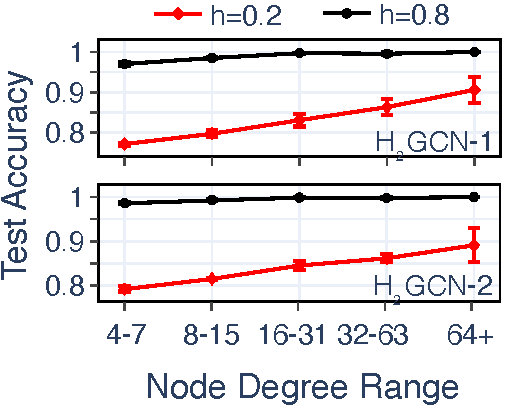
\includegraphics[width=0.28\textwidth]{submissions/Jiong2023/FIG/revisiting-heterophily-GNNs/deg_acc_h2gcn.pdf}
    \caption{\method accuracy per degree range on synthetic heterophilous ($h=0.2$) and homophilous ($h=0.8$) graphs. Figure from \cite{zhu2020beyond}.}
    \label{fig:h2gcn-degree-acc}
\end{wrapfigure}
\paragraph{Summary \& connections to other works.}
From the above analysis, we see that \textbf{the existence of low-degree nodes can lead to weak distinguishability of inter-class NLDs, thus affecting the performance of GCNs}. The significant performance gap between low-degree and high-degree nodes is also observed in \cite{zhu2020beyond},
as shown in Figure~\ref{fig:h2gcn-degree-acc}. 
As a follow-up to our analysis\footnote{These analyses were first made available in the form of a blog post: Zhu, J. and Koutra, D. (2021) Revisiting the problem of heterophily for GNNS. Available at: https://www.jiongzhu.net/revisiting-heterophily-gnns/.}, \citet{ma2021homophily} formalized the effects of node degrees on the distinguishability of NLDs for Contextual Stochastic Block Model (CSBM), and derived a lower bound of node degrees for GCN-style aggregation to improve the distinguishability of NLDs.


\begin{figure}[t]
    \centering
    \begin{subfigure}[t]{0.356\textwidth}
        \adjincludegraphics[width=\textwidth, trim={0.4cm 1cm 2cm 1cm}, clip]{submissions/Jiong2023/FIG/revisiting-heterophily-GNNs/cora-degree.pdf}
        \caption{Degree distribution for \texttt{cora}: it follows a typical power-law degree distribution.}
    \end{subfigure}
    \hspace{0.08\textwidth}
    \begin{subfigure}[t]{0.5\textwidth}
        \adjincludegraphics[width=\textwidth, trim={0.4cm 1cm 2cm 1cm}, clip]{submissions/Jiong2023/FIG/revisiting-heterophily-GNNs/necessity-cora-degree.pdf}
        \caption{Degree distribution of \texttt{necessity-cora}, the cora-based synthetic graphs in \cite{ma2021homophily} with $\gamma=0$ and edge homophily ratio $h\in \{0.077,0.303,0.446,0.584,0.789\}$.}
    \end{subfigure}
    \caption{Degree distributions of \texttt{cora} and \texttt{necessity-cora}. As the level of heterophily increases (i.e., edge homophily ratio $h$ decreases), the degrees for all the nodes increase in \texttt{necessity-cora}, and the degree distributions move further away from the original degree distribution of \texttt{cora}. The shift in degree distribution explains the increase of GCN performance with the level of heterophily for the $\gamma=0$ case in Figure~\ref{fig:revisit-related-observations}(\subref*{fig:revisit-related-observations-necessity-cora}).}
    \label{fig:revisit-cora-necessity-degree}
    \vspace{-0.2cm}
\end{figure}

\paragraph{Revisiting the \texttt{necessity-cora} dataset.} 
The degree distributions of \texttt{necessity-cora} also explain why GCN performance starts to \emph{increase} as the level of homophily $h$ decreases in the range of $h<0.5$ (for noise $\gamma < 0.5$): the \texttt{necessity-cora} graphs with homophily ratio $h<0.5$ have a significantly higher average degree compared to their corresponding base graph \texttt{cora}, as a large amount of edges needs to be added in order to decrease the edge homophily ratio in the (strongly homophilous) base graph. In Figure~\ref{fig:revisit-cora-necessity-degree}, we show the degree distribution of base graph \texttt{cora} in comparison to the degree distributions of the \texttt{necessity-cora} graphs with $\gamma=0$ (i.e., when all the heterophilous edges are added according to the underlying compatibility matrix $\mathcal{D}$, without any randomness) for varying edge homophily ratio $h$. We see that as $h$ decreases, the degrees for all nodes in the graph increase, and the degree distributions move further away from the degree distribution of \texttt{cora}; for the $h=0.077$ instance, even the minimum node degree in the \texttt{necessity-cora} graph has exceeded the degree of most nodes in \texttt{cora}. In our additional empirical analysis (\S\ref{sec:complexity-experiments}), we show that the lack of low-degree nodes is indeed a necessary condition that contributes to the observed high performance of GCNs on \texttt{necessity-cora}.

\subsubsection{Factor (F2): Compatibility Matrices \& Heterophily}
\label{sec:complexity-factor-compatibility}

Another factor that affects the distinguishability of NLDs is the distinguishability of the compatibility matrices for different classes: 
Under the generation process of \texttt{necessity-cora} (\S\ref{sec:complexity-motivating-example}),
when the node degrees are sufficiently high in the generated graphs (Case 2 of \S\ref{sec:complexity-factor-degree}), the NLDs for nodes $v \in \mathcal{V}_c$ are expected to be similar to $\mathcal{D}_c$. 
In this case, the distinguishability of NLDs between nodes in class $c$ and $c'$ mostly depends on the distinguishability of $\mathcal{D}_c$ and $\mathcal{D}_{c'}$, which can also be observed empirically in the compatibility matrices $\mathbf{H}$ of the generated graphs.
In this section, we discuss how complex compatibility patterns in the rows of $\mathbf{H}$ can
reduce the distinguishability of NLDs and contribute to the complexity of heterophily, in addition to (F1) node degrees.



\begin{figure}[t]
    \centering
    \begin{subfigure}[b]{0.31\textwidth}
        \adjincludegraphics[width=\textwidth, trim={0 0 0 {0.13\height}}, clip]{submissions/Jiong2023/FIG/revisiting-heterophily-GNNs/comp-necessity-cora-gamma0.0-h0.165.pdf}
        \caption{Compatibility matrix with $\gamma=0$ and $h=0.16$ in \texttt{necessity-cora}.}
        \label{fig:revisit-comp-matrix-necessity-cora}
    \end{subfigure}
    \hspace{0.02\textwidth}
    \begin{subfigure}[b]{0.31\textwidth}
        \adjincludegraphics[width=\textwidth, trim={0 0 0 {0.13\height}}, clip]{submissions/Jiong2023/FIG/revisiting-heterophily-GNNs/comp-necessity-cora-gamma0.8-h0.163.pdf}
        \caption{Compatibility matrix with $\gamma=0.8$ and $h=0.16$ in \texttt{necessity-cora}.}
    \end{subfigure}
    \hspace{0.02\textwidth}
    \begin{subfigure}[b]{0.31\textwidth}
        \adjincludegraphics[width=\textwidth, trim={0 0 0 {0.13\height}}, clip]{submissions/Jiong2023/FIG/revisiting-heterophily-GNNs/comp-cora-new.pdf}
        \caption{Compatibility matrix of \texttt{cora} with strong homophily.}
        \label{fig:revisit-comp-matrix-cora}
    \end{subfigure}
    \caption{Comparison of compatibility matrices $\matH$ of different synthetic graphs in \texttt{necessity-cora} with homophily ratio $h=0.16$ but different noise ratio $\gamma$, with comparison to the compatibility matrix of \texttt{cora} (the homophilous graph which \texttt{necessity-cora} is based on).}
    \label{fig:revisit-comp-matrices}
\end{figure}

\paragraph{Observations on heterophilous datasets: \texttt{necessity-cora} under different noise levels.} 
The differences in the observed performance of GCN on \texttt{necessity-cora} under different noise levels $\gamma$ (i.e., randomness of the heterophilous edges) in Figure~\ref{fig:revisit-related-observations}(\subref*{fig:revisit-related-observations-necessity-cora}) can be explained by
the differences in the distinguishability of the empirical compatibility matrices $\mathbf{H}$ (and the underlying compatibility matrices $\mathcal{D}$ by extension). In Figure~\ref{fig:revisit-comp-matrices}, we visualize the compatibility matrices of graphs from \texttt{necessity-cora} 
with homophily ratio $h=0.16$, and compare between graphs with noise levels $\gamma=0$ and $\gamma=0.8$:
(1) when $\gamma=0$, the compatibility matrices in \texttt{necessity-cora} are formulated to resemble a ``loop'', where almost all connections for nodes of class $c$ are limited to the two adjacent classes in the ``circle'' of classes (e.g., nodes in Class 2 almost exclusively connect to nodes in Class 1 and 3 in Figure~\ref{fig:revisit-comp-matrices}(\subref*{fig:revisit-comp-matrix-necessity-cora})). 
This ``loop''-pattern helps maintain the high distinguishability of compatibility patterns among different classes, and thus provides an easier node classification problem for GCNs compared to more general heterophilous patterns.
(2) In comparison, when $\gamma=0.8$, the heterophilous connections of class $c$ 
are distributed to all classes $c'\neq c$, and the rows $\mathbf{H}_c$ of the compatibility matrix are less distinct,
which is similar to the case of \texttt{syn-cora} (c.f. Figure~\ref{fig:revisit-dataset-degree-comp}(\subref*{fig:revisit-dataset-degree-comp-syn-cora-comp})).
The high similarity of $\mathbf{H}_c$ among different classes makes it challenging to distinguish different classes from the NLDs even for high-degree nodes, as many heterophilous connections from class $c$ are uniformly distributed to other classes $c'\neq c$. 
This explains the decrease of GCN accuracy under the same homophily level (and degree distribution\footnote{Graphs with the same edge homophily ratio $h$ in \texttt{necessity-cora} also have highly similar degree distributions by extension, since the level of homophily is varied by edge addition.}) in \texttt{necessity-cora} when $\gamma$ increases, as shown in Figure~\ref{fig:revisit-related-observations}(\subref*{fig:revisit-related-observations-necessity-cora}).



\paragraph{Observations on homophilous datasets.} We also note that, echoing the observation in \cite{ma2021homophily}, the \textbf{distinguishability} of the rows in compatibility matrix $\mathbf{H}$ \textbf{is guaranteed for graphs with strong homophily}, as the largest entries in the distributions are concentrated on the diagonal elements of the compatibility matrix $\mathbf{H}$ as shown in Figure~\ref{fig:revisit-comp-matrices}(\subref*{fig:revisit-comp-matrix-cora}). 
\textbf{Thus, the distinguishability of the compatibility matrices is also a challenge specific to heterophilous settings.}

\subsubsection{The Interplay of Degree Distribution, Compatibility Matrices \& NLDs}
\label{sec:complexity-experiments}

In Sections \S\ref{sec:complexity-factor-degree}--\ref{sec:complexity-factor-compatibility}, we discussed two key factors that determine how challenging heterophily is for GNN models. 
Here, we explore the interplay of these factors and NLDs via an empirical study. 
To this end, we construct additional synthetic data with properties complementary to those in \cite{zhu2020beyond,ma2021homophily}. 



\paragraph{Data generation: ``loop''-style schema \& power-law degree distribution.} 
To study the interplay of factors (F1) \& (F2), we generate synthetic graphs which have:
(1) (mostly) %
``loop''-style compatibility matrices (where nodes in each class only connect to nodes in its nearby classes, as if all classes are arranged in a circle), e.g., Figure~\ref{fig:revisit-comp-matrices}(\subref*{fig:revisit-comp-matrix-necessity-cora}).
This schema is similar to that used for \texttt{necessity-cora};
we leverage the same or similar compatibility matrices as specified in \cite{ma2021homophily} in the generation process. (2) the same \emph{power-law} \emph{degree distribution} as \texttt{syn-cora} by following the same modified preferential attachment generation process as in \cite{zhu2020beyond,zhu2021graph}. 

We refer to these synthetic graphs as \texttt{syn-cora-loop}, and consider two variants: \texttt{syn-cora-loop-7} with 7 classes as in \texttt{necessity-cora}, and \texttt{syn-cora-loop-5} with 5 classes as in \texttt{syn-cora}.
In Figure~\ref{fig:revisit-dataset-degree-comp}, we visualize the degree distributions and compatibility matrices of our \texttt{syn-cora-loop} datasets, along with the visualizations for \texttt{necessity-cora} and \texttt{syn-cora}.

\begin{figure}[hbtp]
    \centering
    \begin{subfigure}[b]{0.47\textwidth}
        \adjincludegraphics[width=\textwidth, trim={0 0 0 1.8cm}, clip]{submissions/Jiong2023/FIG/revisiting-heterophily-GNNs/degree-dist-necessity-cora.pdf}
        \caption{Degree distribution of \texttt{necessity-cora} ($\gamma=0$).}
        \label{fig:revisit-dataset-degree-comp-necessity-cora-degree}
    \end{subfigure}
    \hspace{0.04\textwidth}
    \begin{subfigure}[b]{0.47\textwidth}
        \adjincludegraphics[width=\textwidth, trim={0 0 0 1.8cm}, clip]{submissions/Jiong2023/FIG/revisiting-heterophily-GNNs/comp-necessity-cora.pdf}
        \caption{Compatibility matrix of \texttt{necessity-cora} ($\gamma=0$).}
        \label{fig:revisit-dataset-degree-comp-necessity-cora-comp}
    \end{subfigure}
    
    \begin{subfigure}[b]{0.47\textwidth}
        \adjincludegraphics[width=\textwidth, trim={0 0 0 1.6cm}, clip]{submissions/Jiong2023/FIG/revisiting-heterophily-GNNs/degree-dist-necessity-cora-ours-7.pdf}
        \caption{Degree distribution of \texttt{syn-cora-loop-7}.}
    \end{subfigure}
    \hspace{0.04\textwidth}
    \begin{subfigure}[b]{0.47\textwidth}
        \adjincludegraphics[width=\textwidth, trim={0 0 0 1.6cm}, clip]{submissions/Jiong2023/FIG/revisiting-heterophily-GNNs/comp-necessity-cora-ours-7.pdf}
        \caption{Compatibility matrix of \texttt{syn-cora-loop-7}.}
    \end{subfigure}

    \begin{subfigure}[b]{0.47\textwidth}
        \adjincludegraphics[width=\textwidth, trim={0 0 0 1.6cm}, clip]{submissions/Jiong2023/FIG/revisiting-heterophily-GNNs/degree-dist-necessity-cora-ours-5.pdf}
        \caption{Degree distribution of \texttt{syn-cora-loop-5}.}
    \end{subfigure}
    \hspace{0.04\textwidth}
    \begin{subfigure}[b]{0.47\textwidth}
        \adjincludegraphics[width=\textwidth, trim={0 0 0 1.6cm}, clip]{submissions/Jiong2023/FIG/revisiting-heterophily-GNNs/comp-necessity-cora-ours-5.pdf}
        \caption{Compatibility matrix of \texttt{syn-cora-loop-5}.}
    \end{subfigure}

    \begin{subfigure}[b]{0.47\textwidth}
        \adjincludegraphics[width=\textwidth, trim={0 0 0 1.6cm}, clip]{submissions/Jiong2023/FIG/revisiting-heterophily-GNNs/degree-dist-syn-cora.pdf}
        \caption{Degree distribution of \texttt{syn-cora}.}
    \end{subfigure}
    \hspace{0.04\textwidth}
    \begin{subfigure}[b]{0.47\textwidth}
        \adjincludegraphics[width=\textwidth, trim={0 0 0 1.6cm}, clip]{submissions/Jiong2023/FIG/revisiting-heterophily-GNNs/comp-syn-cora.pdf}
        \caption{Compatibility matrix of \texttt{syn-cora}.}
        \label{fig:revisit-dataset-degree-comp-syn-cora-comp}
    \end{subfigure}

    \caption{Synthetic networks used to study the interplay of factors (F1) and (F2).
    \texttt{syn-cora-loop} datasets have the ``loop''-style structure of \texttt{necessity-cora} graphs and the power law degree distribution of the \texttt{syn-cora} graphs.
    }

    \label{fig:revisit-dataset-degree-comp}
\end{figure}




\paragraph{Models.} We assess the influence of degree distributions and compatibility matrices on the performance of three GNN models: \method~\cite{zhu2020beyond}, GCN~\cite{kipf2016semi}, and MLP.
\method represents GNN models that incorporate one or more heterophilous designs as discussed in \S\ref{sec:progress-designs}; we examine two variants of \method, namely \method-1 and \method-2, with one or two layers of aggregation respectively.
In contrast, GCN serves as the GNN baseline model which does not incorporate any heterophilous designs, while MLP functions as the graph-agnostic baseline that does not consider the graph structure.
For GCN, we adopt the same hyperparameter tuning as in \cite{ma2021homophily}, and further tune the dimension of hidden embeddings between 16 and 64.
For \method, we only tune a subset of the hyperparameters that we tune for GCN (16 vs. 112 combinations), which are more hyperparameter combinations than those explored in \cite{zhu2020beyond}.
For each model, we present the mean and standard deviation of the classification accuracy under five runs with different random seeds per dataset.

\paragraph{Data setup.}
Our experiments incorporate four sets of synthetic graphs: \texttt{necessity-cora} provided by \citet{ma2021homophily}, \texttt{syn-cora} from \cite{zhu2020beyond}, and the newly generated \texttt{syn-cora-loop-7} and \texttt{syn-cora-loop-5}.
For \texttt{syn-cora}, we select the graph with homophily level $h=0$; for \texttt{necessity-cora}, we select the graph with noise parameter $\gamma=0$ and $h$ nearest to 0 (i.e., $h=0.03$) as permitted by its generation process. 
We generate \texttt{syn-cora-loop-7} and \texttt{syn-cora-loop-5} with $h=0$. In Table~\ref{tab:revisit-synthetic-results}, we present the statistics for each dataset; the degree distributions and compatibility matrices for all datasets are visualized in Figure~\ref{fig:revisit-dataset-degree-comp}.
For the train/validation/test splits, we utilize the provided splits for \texttt{necessity-cora}~\cite{ma2021homophily}, and create splits for the other datasets using identical sizes as in \texttt{necessity-cora}. Specifically, we randomly select 20 nodes per class for the training set, 500 nodes throughout the graph for the validation set, and allocate the remaining nodes to the test set\footnote{This setup is identical to \cite{kipf2016semi}, but differs from \cite{zhu2020beyond,zhu2021graph} (where Figure~\ref{fig:revisit-related-observations}(\subref*{fig:revisit-related-observations-syn-cora}) was generated), which utilized a larger training set.}.

\begin{table}[t]
\centering
\caption{Dataset statistics and effectiveness of models for node classification. We report the min, median, and max values for the intra-class and inter-CNS, and the mean accuracy $\pm$ standard deviation for each model. The best result for each dataset is highlighted in blue.}
\label{tab:revisit-synthetic-results}
\begin{tabular}{lcccc}
    \toprule
    & \multirow[c]{2}{*}{\shortstack[c]{\textbf{necessity-cora}} } & \multirow[c]{2}{*}{\textbf{syn-cora-loop-7}} & \multirow[c]{2}{*}{\textbf{syn-cora-loop-5}} & \multirow[c]{2}{*}{\textbf{syn-cora}} \\
    \\
    \midrule
    \textbf{\#Nodes} & 2,708 & 2,708 & 1,490 & 1,490 \\
    \textbf{\#Edges} & 132,196 & 5,394 & 2,968 & 2,968 \\
    \textbf{\# Classes} & 7 & 7 & 5 & 5 \\
    \textbf{Edge Hom.} $h$ & 0.03 & 0 & 0 & 0 \\
    \midrule
    \textbf{(F1) High-degree Nodes Only} & \cmark & \xmark & \xmark & \xmark \\
    \textbf{(F2) Compatibility ``Loop''} & \cmark & \cmark & \cmark & \xmark \\
    \textbf{Heterophily Type} & Easy & Challenging & Challenging & Most challenging \\
    \midrule
    \textbf{Agg. Hom.} $h_{\mathrm{agg}}$ & 1.00 & 0.90 & 1.00 & 0.41 \\  %
    \textbf{Intra-CNS} {\small (min/median/max)} & 0.97/0.99/1.00 & 0.79/0.82/0.84 & 0.78/0.80/0.80 & 0.62/0.63/0.64 \\ %
    \textbf{Inter-CNS} {\small (min/median/max)} & 0.00/0.08/0.52 & 0.00/0.31/0.57 & 0.30/0.39/0.47 & 0.53/0.57/0.60 \\ %

    \midrule
    \midrule
    \method-2 & $99.26\pm0.28$ & \cellcolor{blue!20}$88.45\pm1.26$ & \cellcolor{blue!20}$87.98\pm1.49$ & \cellcolor{blue!20}$68.95\pm1.88$ \\
    \method-1 & $93.48\pm0.93$ & $80.85\pm1.69$ & $82.40\pm1.77$ & $66.82\pm2.13$ \\
    GCN & \cellcolor{blue!20}$100.00\pm 0.00$ & $65.10\pm1.80$ & $59.26\pm2.17$ & $27.27\pm1.72$ \\
    MLP & $59.16\pm0.52$ & $58.20\pm2.05$ & $64.16\pm1.61$ & $63.84 \pm2.17$ \\
    \bottomrule
\end{tabular}
\end{table}

\paragraph{GNN performance \& graph properties.} In Table~\ref{tab:revisit-synthetic-results}, we list the performance of each model along with the corresponding properties of the graphs.
We observe the effects of the interplay between low-degree nodes and more complex compatibility matrices to the performance of GNN models when the graphs share similar edge homophily ratio $h$ (0 or as close to 0 as the generation process allows):
\begin{enumerate}[label=(\arabic*),nosep]
\item On \texttt{necessity-cora}, with no low-degree nodes and the simpler ``loop''-style compatibility matrices (Figure~\ref{fig:revisit-dataset-degree-comp}(\subref*{fig:revisit-dataset-degree-comp-necessity-cora-degree})-(\subref*{fig:revisit-dataset-degree-comp-necessity-cora-comp})), models like GCN and \method-2 can achieve near-perfect accuracy.

\item On \texttt{syn-cora-loop} variants, where we keep the ``loop''-style compatibility matrices but modify the degree distributions to follow a power law, we observe 34.90\% to 40.74\% decrease in accuracy for GCN, which falls below the accuracy of \method. As we discussed in \S\ref{sec:complexity-factor-degree}, this heterophilous case is challenging; this is also confirmed by the performance drop for the graph-aware methods, including \method. 

\item On \texttt{syn-cora}, which further strips the ``loop''-style compatibility matrices for heterophilous connections and has more complex connectivity patterns across different classes, the performance of GCN further decreases by 31.99\% and falls much below the performance of the graph-agnostic MLP in this case; though the accuracy of \method variants also decreases significantly in this challenging case, they still outperform MLP in this case.
\end{enumerate}

\paragraph{NLD distinguishability \& graph properties.} The significant changes in the accuracy of GCN can also be explained by the changes in the distinguishability of NLDs caused by different graph properties.
In Table~\ref{tab:revisit-synthetic-results}, we report the Class Neighborhood Similarity (CNS) and Graph Aggregation Homophily $h_{\mathrm{agg}}$ for the all synthetic graphs (as defined in \S\ref{sec:complexity-measurements}, where
we consider self-loops in accordance with GCN aggregation). 
We also visualize the CNS and its standard deviation (following Eq.~\eqref{eq:complexity-CNS}) between pairs of classes on each dataset in Figure~\ref{fig:revisit-dataset-CNS}. 

\begin{figure}[t]
    \centering
    \begin{subfigure}[b]{0.47\textwidth}
        \adjincludegraphics[width=\textwidth, trim={0 0 0 {0.25\height}}, clip]{submissions/Jiong2023/FIG/revisiting-heterophily-GNNs/cross-class-sim-necessity-cora.pdf}
        \caption{CNS of \texttt{necessity-cora} with $\gamma=0$.}
    \end{subfigure}
    \hspace{0.04\textwidth}
    \begin{subfigure}[b]{0.47\textwidth}
        \adjincludegraphics[width=\textwidth, trim={0 0 0 {0.25\height}}, clip]{submissions/Jiong2023/FIG/revisiting-heterophily-GNNs/cross-class-sim-necessity-cora-ours-7.pdf}
        \caption{CNS of \texttt{syn-cora-loop-7}.}
    \end{subfigure}

    \begin{subfigure}[b]{0.47\textwidth}
        \adjincludegraphics[width=\textwidth, trim={0 0 0 {0.25\height}}, clip]{submissions/Jiong2023/FIG/revisiting-heterophily-GNNs/cross-class-sim-necessity-cora-ours-5.pdf}
        \caption{CNS of \texttt{syn-cora-loop-5}.}
    \end{subfigure}
    \hspace{0.04\textwidth}
    \begin{subfigure}[b]{0.47\textwidth}
        \adjincludegraphics[width=\textwidth, trim={0 0 0 {0.25\height}}, clip]{submissions/Jiong2023/FIG/revisiting-heterophily-GNNs/cross-class-sim-syn-cora.pdf}
        \caption{CNS of \texttt{syn-cora}.}
    \end{subfigure}
    \caption{Class neighborhood similarities (CNS) of the synthetic datasets in Table~\ref{tab:revisit-synthetic-results}.}
    \label{fig:revisit-dataset-CNS}
\end{figure}

Based on the intra-class and inter-CNS in Table~\ref{tab:revisit-synthetic-results}, we observe that:
\begin{enumerate}[label=(\arabic*)]
\item With the presence of low-degree nodes, the \texttt{syn-cora-loop} variants have reduced intra-CNS with higher variances compared to \texttt{necessity-cora}, while the inter-CNS also increases, though they share similar ``loop''-style compatibility matrices;
\item The removal of the ``loop'' pattern in the compatibility matrices of \texttt{syn-cora} further reduces the intra-CNS to a level similar to the inter-CNS, which leads to weak distinguishability of the neighborhood label distributions between nodes from different classes. 
These observations explain the decrease of GCN performance observed in our experiments, and show how that the distinguishability of the neighborhood label distributions can depend on other properties like degree distributions and class compatibility matrices in the underlying graphs.
\end{enumerate}

Additionally, we note that while the Aggregation Homophily $h_{\mathrm{agg}}$ is a good indicator of the performance of GCN on \texttt{necessity-cora} and \texttt{syn-cora}, it does not correlate well with the performance changes of GCN on \texttt{syn-cora-loop} variants. 
While $h_{\mathrm{agg}}$ is defined as the \emph{ratio} of nodes with NLD more similar %
to nodes from the same class than nodes from other classes (Eq. \eqref{eq:complexity-gah}), it does not measure the \emph{level of similarity} between the NLDs of nodes from the same or different classes as CNS does. Therefore, we believe that CNS is a more accurate and comprehensive indicator of the complexity of heterophily, as Table~\ref{tab:revisit-synthetic-results} shows. 

\paragraph{Effectiveness of heterophilous GNN designs.} 
With \method as an example that incorporates three heterophilous designs (D1), (D2) and (D3) (discussed in \S\ref{sec:progress-designs}),
we observe that these heterophilous designs can largely improve the performance of GNNs compared to GCNs even when the heterophilous connections do not have the ideal distinguishability in the NLDs as in the \texttt{necessity-cora} ($\gamma=0$) case.
When the distinguishability of NLDs among different classes is low (i.e., when intra-CNS is low and inter-CNS is high), the \method variants largely outperform GCN under heterophilous settings. 
While our experiments focus more on the effects of graph properties to NLD distinguishability and GNN performance and only considered \method as an example for heterophilous GNNs, more comprehensive experiments have been conducted in recent works \cite{platonov2023critical,yan2022two,lim2021large} which support the effectiveness of these heterophilous GNN designs. 


\section{Conclusion \& Future Directions}
\label{sec:conclusion}

In this work, we revisited the debate of whether heterophily is a challenge for GNNs. 
We first reviewed representative architectural designs that have been proposed in the literature for improving the performance of GNNs on heterophilous data, and then discussed the connections with other objectives of GNN research, such as robustness, fairness, and reducing oversmoothing. 
To address the debate and reconcile seemingly contradictory statements in the literature, we conducted an extensive empirical analysis that aimed to provide a better understanding of when heterophily is challenging and when it does not pose significant additional challenges compared to handling graphs with homophily. 
We also considered recently proposed measures for quantifying the complexity of heterophily and evaluated their effectiveness across synthetic datasets based on different generation processes. 
Our analysis revealed two key factors that increase the complexity of heterophily: (F1) the presence of low-degree nodes, and (F2) the complexity of the class compatibility matrices of the underlying graphs. 
These factors present unique challenges for GNNs under heterophilous settings, and necessitate architectural designs that can improve the performance of GNNs. 
We hope that our review and empirical analysis will inspire future research 
on better understanding the unique challenges of heterophily in GNNs and  developing more effective GNN models that can handle well both graphs with homophily and heterophily (of variable complexity).



\paragraph{Future Directions.} There are many promising research directions towards understanding the unique challenges that heterophily poses to GNN models.
Next we discuss some representative open problems: 
\setlist{leftmargin=*}
\begin{itemize}
    \item \textbf{Beyond node classification and global homophily.} 
    Most existing works on GNNs and heterophily (including the ones we review in this work) focus on node classification, where heterophily can be defined and measured with respect to the agreement of class labels for connected nodes. 
    However, many important applications on graphs, such as recommendation systems, query matching, and the prediction of molecular properties, are based on other learning tasks such as link prediction and graph classification. 
    It is thus important to understand the effects of heterophily on these tasks and inform the design of tailored GNN models that can handle heterophily.
    While few works have discussed heterophily in the settings of link prediction~\cite{zhou2022link,zhu2023simplifying} and graph classification~\cite{ye2022incorporating}, their definition of heterophily is still based on node class labels, which are often not available for these tasks.
    Measuring homophily in the absence of node is an interesting problem for these graph learning tasks. 
    Moreover, going beyond a global perspective and exploring the effect of different mixing patterns across different neighborhoods is an important research direction that has started to gain reaction~\cite{loveland2022graph}. 
    
    \item \textbf{More datasets \& applications.} Despite recent efforts in collecting and introducing new datasets that address the drawbacks of existing heterophilous ones~\cite{lim2021large,platonov2023critical}, we believe that the call for more heterophilous graph datasets and applications is still important and timely. 
    Many existing works on GNN and heterophily rely on the six heterophilous graph datasets which were first adopted by \citet{Pei2020Geom-GCN}. 
    While these datasets were useful during the early stages of research on GNNs and heterophily, multiple works~\cite{zhu2020beyond,lim2021large,platonov2023critical} have pointed out the drawbacks of these commonly adopted benchmark datasets, namely their small sizes, artificial class labels, imbalanced class sizes, unusual network structure, and even leakage of test nodes in the training set. 
    In light of these, \citet{lim2021large} and \citet{platonov2023critical} proposed a set of mid- to large-scale social, citation and web networks with more diverse node features and realistic class labels, 
    but these datasets have yet to gain widespread adoption,
    and the relationship between the (heterophilous) links and the class labels is often ambiguous   
    (e.g., predicting product ratings on Amazon based on edges connecting frequently bought items). 
    Thus, we believe that there is still a need for datasets that have naturally-occurring heterophilous connections that align better with defined node class labels. 
    In terms of application domains, it would be useful to go beyond social, citation, and webpage networks and introduce benchmarks that capture 
    molecular or protein structures, which could also aid the investigation of more graph learning tasks that we discuss above. 
    
    \item \textbf{Connections between heterophily \& heterogeneity.} 
    Although we highlighted in \S\ref{sec:preliminaries} that heterophily and heterogeneity are two distinct concepts that should not be confused, heterogeneity may introduce unique forms and challenges of heterophily that are worth investigating: connected nodes of different \emph{types} could imply dissimilarity in their embeddings, resembling the concept of heterophily, while the level of homophily may also vary across different local mixing patterns. As a result, GNN models operating on heterogeneous graphs have already adopted designs similar to those tailored for heterophily, such as the separation of ego- and neighbor-embeddings and the use of type-specific kernels in message passing~\cite{schlichtkrull2018modeling}, in order to address the challenges of heterogeneity. Moreover, recently, \citet{guo2023homophily} also discussed how enhancing the homophily level in the meta-paths of heterogeneous graphs can improve GNN performance. Therefore, we believe that further research on the connections between heterophily and heterogeneity can help better understand the connections between the methodologies and findings of these two settings, which in turn may lead to the development of more effective GNNs for both scenarios.
\end{itemize}







\section*{Acknowledgements}
We thank Yao Ma, Xiaorui Liu, Neil Shah and Jiliang Tang for sharing the synthetic datasets generated in \cite{ma2021homophily} and the constructive discussions regarding the takeaways of our analysis in \S\ref{sec:complexity}. This material is based upon work supported by the National Science Foundation under IIS 2212143,  CAREER Grant No.~IIS 1845491,  IIS 1452425, 
an Adobe Digital Experience research faculty award, an Amazon faculty award, a Google faculty award, 
and AWS Cloud Credits for Research. We gratefully acknowledge the support of NVIDIA Corporation with the donation of the Quadro P6000 GPU used for this research. 
Any opinions, findings, and conclusions or recommendations expressed in this material are those of the author(s) and do not necessarily reflect the views of the National Science Foundation or other funding parties.





{
\small
\bibliographystyle{plain}
\bibliography{submissions/Jiong2023/PAGES/BIB/main,submissions/Jiong2023/PAGES/BIB/all}
}

\appendix
\newpage




\end{document}

\end{article}
\begin{article}
{A Survey on Explainability of Graph Neural Networks}
{Jaykumar Kakkad, Jaspal Jannu, Kartik Sharma, Charu Aggarwal, Sourav Medya}
\pdfminorversion=5
\documentclass[11pt]{article}
\usepackage{deauthor,times,graphicx,caption,microtype}
\usepackage{hyperref}
\usepackage{listings}
\usepackage{booktabs}

\begin{document}

\title{Optimistic Lock Coupling: A Scalable and Efficient General-Purpose Synchronization Method}

\author{Viktor Leis, Michael Haubenschild\raisebox{0.9ex}{$\ast$}, Thomas Neumann\\ Technische Universit{\"a}t M{\"u}nchen \hspace{0.7cm} Tableau Software\raisebox{0.9ex}{$\ast$} \\ {\{leis,neumann\}{@}in.tum.de} \hspace{0.7cm} {mhaubenschild{@}tableau.com\raisebox{0.9ex}{$\ast$}}}

\maketitle

\begin{abstract}
As the number of cores on commodity processors continues to increase, scalability becomes more and more crucial for overall performance.
Scalable and efficient concurrent data structures are particularly important, as these are often the building blocks of parallel algorithms.
Unfortunately, traditional synchronization techniques based on fine-grained locking have been shown to be unscalable on modern multi-core CPUs.
Lock-free data structures, on the other hand, are extremely difficult to design and often incur significant overhead.

In this work, we make the case for Optimistic Lock Coupling as a practical alternative to both traditional locking and the lock-free approach.
We show that Optimistic Lock Coupling is highly scalable and almost as simple to implement as traditional lock coupling.
Another important advantage is that it is easily applicable to most tree-like data structures.
We therefore argue that Optimistic Lock Coupling, rather than a complex and error-prone custom synchronization protocol, should be the default choice for performance-critical data structures.
\end{abstract}

\section{Introduction}

% more and more cores
Today, Intel's commodity server processors have up to 28 cores and its upcoming microarchitecture will have up to 48 cores per socket~\cite{intel}.
Similarly, AMD currently stands at 32 cores and this number is expected to double in the next generation~\cite{amd}.
Since both platforms support simultaneous multithreading (also known as hyperthreading), affordable commodity servers (with up to two sockets) will soon routinely have between 100 and 200 hardware threads.

% data structure scalability is important
With such a high degree of hardware parallelism, efficient data processing crucially depends on how well concurrent data structures scale.
Internally, database systems use a plethora of data structures like table heaps, internal work queues, and, most importantly, index structures.
Any of these can easily become a scalability (and therefore overall performance) bottleneck on many-core CPUs.

% traditional synchronization: fine-grained locks, slow, cache invalidation
Traditionally, database systems synchronize internal data structures using fine-grained reader/writer locks\footnote{In this work, we focus on data structure synchronization rather than high-level transaction semantics and therefore use the term {\em lock} for what would typically be called {\em latch} in the database literature. We thus follow common computer science (rather than database) terminology.}.
Unfortunately, while fine-grained locking makes lock contention unlikely, it still results in bad scalability because lock acquisition and release require writing to shared memory.
Due to the way cache coherency is implemented on modern multi-core CPUs, these writes cause additional cache misses\footnote{The cache coherency protocol ensures that all copies of a cache line on other cores are invalidated before the write can proceed.} and the cache line containing the lock's internal data becomes a point of physical contention.
As a result, any frequently-accessed lock (e.g., the lock of the root node of a B-tree) severely limits scalability.

% lock-free bw-tree: no more latches, but indirections, extremely complex
Lock-free data structures like the Bw-tree~\cite{DBLP:conf/icde/LevandoskiLS13a} (a lock-free B-tree variant) or the Split-Ordered List~\cite{DBLP:journals/jacm/ShalevS06} (a lock-free hash table) do not acquire any locks and therefore generally scale much better than locking-based approaches (in particular for read-mostly workloads).
However, lock-free synchronization has other downsides:
First, it is very difficult and results in extremely complex and error-prone code (when compared to locking).
Second, because the functionality of atomic primitives provided by the hardware (e.g., atomically compare-and-swap 8 bytes) is limited, complex operations require additional indirections within the data structure.
For example, the Bw-tree requires an indirection table and the Split-Ordered List requires ``dummy nodes'', resulting in overhead due to additional cache misses.

% OLC for the win
In this paper we make the case for {\em Optimistic Lock Coupling (OLC)}, a synchronization method that combines some of the best properties of lock-based and lock-free synchronization.
OLC utilizes a special lock type that can be used in two modes:
The first mode is similar to a traditional mutex and excludes other threads by physically acquiring the underlying lock.
In the second mode, reads can proceed optimistically by validating a version counter that is embedded in the lock (similar to optimistic concurrency control).
The first mode is typically used by writers and the second mode by readers.
Besides this special lock type, OLC is based on the observation that optimistic lock validations can be interleaved/coupled---similar to the pair-wise interleaved lock acquisition of traditional lock coupling.
Hence, the name Optimistic Lock Coupling.

OLC has a number of desirable features:
\begin{itemize}
\item By reducing the number of writes to shared memory locations and thereby avoiding cache invalidations, it {\bf scales well} for most workloads.
\item In comparison to unsynchronized code, it requires few additional CPU instructions making it {\bf efficient}.
\item OLC is {\bf widely applicable} to different data structures. It has already been successfully used for synchronizing binary search trees~\cite{DBLP:conf/ppopp/BronsonCCO10}, tries~\cite{artsync}, trie/B-tree hybrids~\cite{DBLP:dblp_conf/eurosys/MaoKM12}, and B-trees~\cite{buzzword}.
\item In comparison to the lock-free paradigm, it is also {\bf easy to use} and requires few modifications to existing, single-threaded data structures.
\end{itemize}
Despite these positive features and its simplicity, OLC is not yet widely known.
The goal of this paper is therefore to popularize this simple idea and to make a case for it.
We argue that OLC deserves to be widely known.
It is a good default synchronization paradigm---more complex, data structure-specific protocols are seldom beneficial.

The rest of the paper is organized as follows.
Section~\ref{sec:related} discusses related work, tracing the history of OLC and its underlying ideas in the literature.
The core of the paper is Section~\ref{sec:olc}, which describes the ideas behind OLC and how it can be used to synchronize complex data structures.
In Section~\ref{sec:evaluation} we experimentally show that OLC has low overhead and scales well when used to synchronize an in-memory B-tree.
We summarize the paper in Section~\ref{sec:conc}.

\newpage
\section{Related Work}\label{sec:related}

Lock coupling has been proposed as a method for allowing concurrent operations on B-trees in 1977~\cite{DBLP:journals/acta/BayerS77}.
This traditional and still widely-used method, described in detail in Graefe's B-tree survey~\cite{DBLP:journals/ftdb/Graefe11}, is also called ``latch coupling'', ``hand-over-hand locking'', and ``crabbing''.
Because at most two locks are held at-a-time during tree traversal, this technique seemingly allows for a high degree of parallelism---in particular if read/write locks are used to enable inner nodes to be locked in shared mode.
However, as we show in Section~\ref{sec:evaluation}, on modern hardware lock acquisition (even in shared mode) results in suboptimal scalability.

An early alternative from 1981 is a B-tree variant called B-link tree~\cite{DBLP:journals/tods/LehmanY81}, which only holds a single lock at a time.
It is based on the observation that between the release of the parent lock and the acquisition of the child lock, the only ``dangerous'' thing that could have happened is the split of a child node (assuming one does not implement merge operations).
Thus, when a split happens, the key being searched might end up on a neighboring node to the right of the current child node.
A B-link tree traversal therefore detects this condition and, if needed, transparently proceeds to the neighboring node.
Releasing the parent lock early is highly beneficial when the child node needs to be fetched from disk.
For in-memory workloads, however, the B-link tree has the same scalability issues as lock coupling (it acquires just as many locks).

The next major advance, Optimistic Latch-Free Index Traversal (OLFIT)~\cite{DBLP:conf/vldb/ChaHKK01}, was proposed in 2001.
OLFIT introduced the idea of a combined lock/update counter, which we call {\em optimistic lock}. % , for lack of a better name,
Based on these per-node optimistic locks and the synchronization protocol of the B-link tree, OLFIT finally achieves good scalability on parallel processors.
The OLFIT protocol is fairly complex, as it requires both the non-trivial B-link protocol and optimistic locks.
Furthermore, like the B-link tree protocol, it does not support merging nodes, and is specific to B-trees (cannot easily be applied to other data structures).

In the following two decades, the growth of main-memory capacity led to much research into other data structures besides the venerable B-tree.
Particularly relevant for our discussion is Bronson et al.'s~\cite{DBLP:conf/ppopp/BronsonCCO10} concurrent binary search tree, which is based on optimistic version validation and has a sophisticated, data structure-specific synchronization protocol.
To the best of our knowledge, this 2010 paper is the first that, as part of its protocol, interleaves version validation across nodes---rather than validating each node separately like OLFIT.
In that paper, this idea is called ``hand-over-hand, optimistic validation'', while we prefer the term Optimistic Lock Coupling to highlight the close resemblance to traditional lock coupling.
Similarly, Mao et al.'s~\cite{DBLP:dblp_conf/eurosys/MaoKM12} Masstree (a concurrent hybrid trie/B-tree) is also based on the same ideas, but again uses them as part of a more complex protocol.

The Adaptive Radix Tree (ART)~\cite{art} is another recent in-memory data structure, which we proposed in 2013.
In contrast to the two data structures just mentioned, it was originally designed with single-threaded performance in mind without supporting concurrency.
To add support for concurrency, we initially started designing a custom protocol called Read-Optimized Write Exclusion (ROWEX)~\cite{artsync}, which turned out to be non-trivial and requires modifications of the underlying data structure\footnote{Note that ROWEX is already easier to apply to existing data structures than the lock-free approach. The difficulty depends on the data structure. Applying ROWEX is hard for B-trees with sorted keys and fairly easy for copy-on-write data structures like the Height Optimized Trie~\cite{hot}---with ART being somewhere in the middle.}.
However, fairly late in the project, we also realized, that OLC {\em alone} (rather than as part of a more complex protocol) is sufficient to synchronize ART.
No other changes to the data structure were necessary.
Both approaches were published and experimentally evaluated in a followup paper~\cite{artsync}, which shows that, despite its simplicity, OLC is efficient, scalable, and generally outperforms ROWEX.

Similar results were recently published regarding B-trees~\cite{buzzword}.
In this experimental study a simple OLC-based synchronization outperformed the Bw-tree~\cite{DBLP:conf/icde/LevandoskiLS13a}, a complex lock-free synchronization approach.
Another recent paper shows that for write-intensive workloads, locking often performs better than lock-free synchronization~\cite{DBLP:conf/cidr/FaleiroA17}.
These experiences indicate that OLC is a general-purpose synchronization paradigm and motivate the current paper.

%foster b-tree\cite{DBLP:journals/tods/GraefeKK12}
%Shasha theory~\cite{DBLP:journals/tods/ShashaG88}

\section{Optimistic Lock Coupling}\label{sec:olc}

% locks suck
The standard technique for inter-thread synchronization is mutual exclusion using fine-grained locks.
In a B-tree, for example, every node usually has its own associated lock, which is acquired before accessing that node.
The problem of locking on modern multi- and many-core processors is that lock acquisition and release require writing to the shared memory location that implements the lock.
This write causes exclusive ownership of the underlying cache line and invalidates copies of it on all other processor cores.
For hierarchical, tree-like data structures, the lock of the root node becomes a point of physical contention---even in read-only workloads and even when read/write locks are used.
Depending on the specific data structure, number of cores, cache coherency protocol implementation, cache topology, whether Non-Uniform Memory Access (NUMA) is used, locking can even result in multi-threaded performance that is worse than single-threaded execution.

% in b-trees this happens very much
The inherent pessimism of locking is particularly unfortunate for B-trees:
Despite the fact that logical modifications of the root node are very infrequent, every B-tree operation must lock the root node during tree traversal\footnote{To a lesser extent this obviously applies to all inner nodes, not just the root.}.
Even the vast majority of update operations (with the exception of splits and merges), only modify a single leaf node.
These observations indicate that a more optimistic approach, which does not require locking inner nodes, would be very beneficial for B-trees.

\subsection{Optimistic Locks}

% optimism to the rescue
As the name indicates, optimistic locks try to solve the scalability issues of traditional locks using an optimistic approach.
Instead of always physically acquiring locks, even for nodes that are unlikely to be modified simultaneously, after-the-fact validation is used to detect conflicts.
This is done by augmenting each lock with a version/update counter that is incremented on every modification.
Using this version counter, readers can optimistically proceed before validating that the version did not change to ensure that the read was safe.
If validation fails, the operation is restarted.

% details on opt locks
Using optimistic locks, a read-only node access (i.e., the majority of all operations in a B-tree) does not acquire the lock and does not increment the version counter.
Instead, it performs the following steps:
\begin{enumerate}
\item read lock version (restart if lock is not free)
\item access node
\item read the version again and validate that it has not changed in the meantime
\end{enumerate}
If the last step (the validation) fails, the operation has to be restarted.
Write operations, on the other hand, are more similar to traditional locking:
\begin{enumerate}
\item acquire lock (wait if necessary)
\item access/write to node
\item increment version and unlock node
\end{enumerate}
Writes can therefore protect a node from other writes.

% similar to locks
As we observed in an earlier paper~\cite{artsync}, because of similar semantics, optimistic locks can be hidden behind an API very similar to traditional read/write locks.
Both approaches have an exclusive lock mode, and acquiring a traditional lock in shared mode is analogous to optimistic version validation.
Furthermore, like with some implementations of traditional read/write locks, optimistic locks allow upgrading a shared lock to an exclusive lock.
Lock upgrades are, for example, used to avoid most B-tree update operations from having to lock inner nodes.
In our experience, the close resemblance of optimistic and traditional locks simplifies the reasoning about optimistic locks;
one can apply similar thinking as in traditional lock-based protocols.

\subsection{Lock Coupling with Optimistic Locks}

\begin{figure}
  \centering
  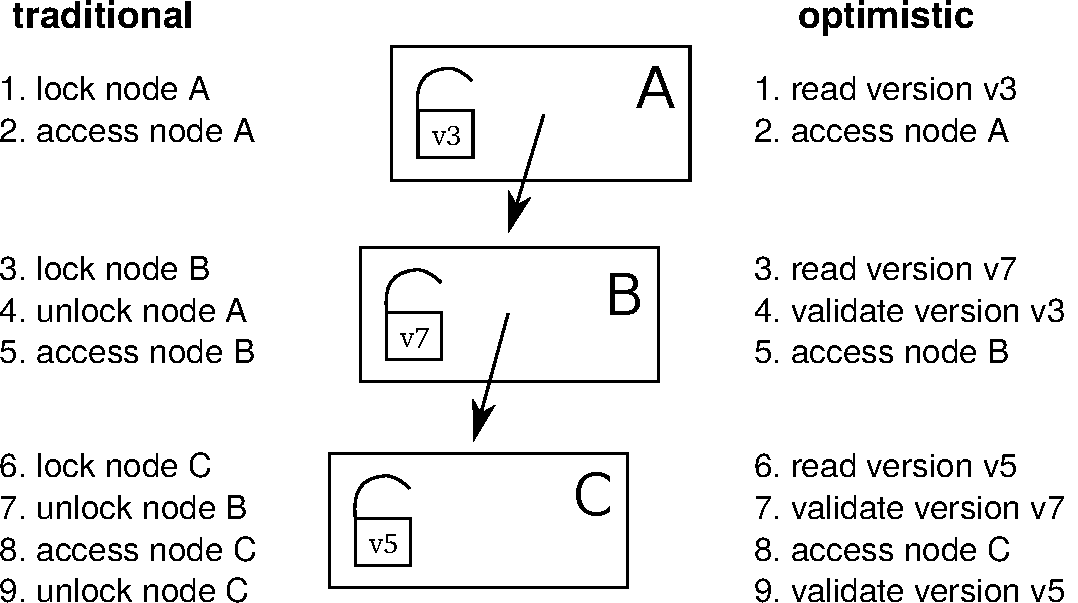
\includegraphics[width=0.65\linewidth]{olcall.pdf}
  \vspace{0.2cm}
  \caption{Comparison of a lookup operation in a 3-level tree using traditional lock coupling (left-hand side) vs.~optimistic lock coupling (right-hand side).}
  \label{fig:olc}
\end{figure}

The traditional and most common lock-based synchronization protocol for B-trees is lock coupling, which interleaves lock acquisitions while holding at most two locks at a time.
If, as we observed earlier, optimistic locks have similar semantics as traditional locks, it is natural to ask whether lock coupling can be combined with optimistic locks.
And indeed the answer is yes: One can almost mechanically translate traditional lock coupling code to optimistic lock coupling code.
This is illustrated in Figure~\ref{fig:olc}, which compares the traversal in a tree of height 3 using traditional and optimistic locks.
As the figure shows, the main difference is that locking is translated to reading the version and that unlocking becomes validation of the previously read version.
This simple change provides efficient lock-free tree traversal without the need to design a complex synchronization protocol.

It is important to emphasize the conceptual simplicity of OLC in comparison to data structures that use custom protocols like the Bw-tree~\cite{DBLP:conf/icde/LevandoskiLS13a}.
To implement lock-free access, the Bw-tree requires an indirection table, delta nodes, complex splitting and merging logic, retry logic, etc.
OLC, on the other hand, can directly be applied to B-trees mostly by adding the appropriate optimistic locking code and without modifying the node layout itself.
Therefore, OpenBw-Tree, an open source implementation of the Bw-tree, requires an order of magnitude more code than a B-tree based on OLC\footnote{Both implementations are available on GitHub: \url{https://github.com/wangziqi2016/index-microbench}}.
Given how difficult it is to develop, validate, and debug lock-free code, simplicity is obviously a major advantage.

\subsection{Correctness Aspects}

\begin{figure}
  % \centering
  %[basicstyle=\normalsize\ttfamily,showstringspaces=false,columns=fullflexible,breaklines=false,breakatwhitespace=true,numbers=none,numberstyle=\small,style=C,keepspaces=true]
\begin{lstlisting}[basicstyle=\ttfamily,language=C++,numbers=left,numberstyle=\small]
std::atomic<BTreeNode*> root;

// search for key in B+tree, returns payload in resultOut
bool lookup(Key key, Value& resultOut) {
   BTreeNode* node = root.load();
   uint64_t nodeVersion = node->readLockOrRestart();
   if (node != root.load()) // make sure the root is still the root
      restart();

   BTreeInner<Key>* parent = nullptr;
   uint64_t parentVersion = 0;

   while (node->isInner()) {
      auto inner = (BTreeInner*)node;

      // unlock parent and make current node the parent
      if (parent)
         parent->readUnlockOrRestart(parentVersion);
      parent = inner;
      parentVersion = nodeVersion;

      // search for next node
      node = inner->findChild(key);
      // validate 'inner' to ensure that 'node' pointer is valid
      inner->checkOrRestart(nodeVersion);
      // now it safe to dereference 'node' pointer (read its version)
      nodeVersion = node->readLockOrRestart();
   }

   // search in leaf and retrieve payload
   auto leaf = (BTreeLeaf*)node;
   bool success = leaf->findValue(key, resultOut);

   // unlock everything
   if (parent)
      parent->readUnlockOrRestart(parentVersion);
   node->readUnlockOrRestart(nodeVersion);

   return success;
}
\end{lstlisting}
  \vspace{0.2cm}
  \caption{B-tree lookup code using OLC. For simplicity, the restart logic is not shown.}
  \label{fig:lookup}
\end{figure}

So far, we have introduced the high-level ideas behind OLC and have stressed its similarity to traditional lock coupling.
Let us now discuss some cases where the close similarity between lock coupling and OLC breaks down.
To make this more concrete, we show the B-tree lookup code in Figure~\ref{fig:lookup}.
In the code, \texttt{readLockOrRestart} reads the lock version and \texttt{readUnlockOrRestart} validates that the read was correct.

One issue with OLC is that any pointer speculatively read from a node may point to invalid memory (if that node is modified concurrently).
Dereferencing such a pointer (e.g., to read its optimistic lock), may cause a segmentation fault or undefined behavior.
In the code shown in Figure~\ref{fig:lookup}, this problem is prevented by the extra check in line 25, which ensures that the read from the node containing the pointer was correct.
Without this additional validation, the code would in line 27 dereference the pointer speculatively read in line 23.
Note that the implementation of \texttt{checkOrRestart} is actually identical to \texttt{readUnlockOrRestart}.
We chose to give it a different name to highlight the fact that this extra check would not be necessary with read/write locks.

Another potential issue with optimistic locks is code that does not terminate.
Code that speculatively accesses a node, like an intra-node binary search, should be written in a way such that it always terminates---even in the presence of concurrent writes.
Otherwise, the validation code that detects the concurrent write will never run.
The binary search of a B-tree, for example, needs to be written in such a way that each comparison makes progress.
For some data structures that do not require loops in the traversal code (like ART) termination is trivially true.

\subsection{Implementation Details}

% implementation, efficiency
To implement an optimistic lock, one can combine the lock and the version counter into a single 64-bit\footnote{Even after subtracting one bit for the lock status, a back-of-the-envelope calculation can show that 63 bits are large enough to never overflow in practice.} word~\cite{artsync}.
A typical read operation will therefore merely consist of reading this version counter atomically.
In C++11 this can be implemented using the \texttt{std::atomic} type.

On x86, atomic reads are cheap because of x86's strong memory order guarantees.
No memory fences are required for sequentially-consistent loads, which are translated (by both GCC and clang) into standard \texttt{MOV} instructions.
Hence, the only effect of \texttt{std::atomic} for loads is preventing instruction re-ordering.
This makes version access and validation cheap.
Acquiring and releasing an optimistic lock in exclusive mode has comparable cost to a traditional lock:
A fairly expensive sequentially-consistent store is needed for acquiring a lock, while a standard \texttt{MOV} suffices for releasing it.
A simple sinlock-based implementation of optimistic locks can be found in the appendix of an earlier paper~\cite{artsync}.

OLC code must be able to handle restarts since validation or lock upgrade can fail due to concurrent writers.
Restarts can easily be implemented by wrapping the data structure operation in a loop (for simplicity not shown in Figure~\ref{fig:lookup}).
Such a loop also enables limiting the number of optimistic retry operations and falling back to pessimistic locking in cases of very heavy contention.
The ability to fall back to traditional locking is a major advantage of OLC in terms of robustness over lock-free approaches, which do not have this option.

In addition to the optimistic shared mode and the exclusive mode, optimistic locks also support a ``shared pessimistic'' mode, which physically acquires the lock in shared mode (allowing multiple concurrent readers but no writers).
This mode is useful for table (or range) scans that touch many tuples on a leaf page (which would otherwise easily abort).
Finally, let us mention that large range scans and table scans, should be broken up into several per-node traversals as is done in the LeanStore~\cite{leanstore} system.

Like all lock-free data structures, but unlike traditional locking and Hardware Transactional Memory~\cite{DBLP:conf/hpca/KarnagelDRLLSL14,DBLP:journals/pvldb/MakreshanskiLS15,htmtkde}, OLC requires care when deleting (and reusing) nodes.
The reason is that a deleting thread can never be sure that a node can be reclaimed because other threads might still be optimistically reading from that node.
Therefore, standard solutions like epoch-based reclamation~\cite{DBLP:conf/sosp/TuZKLM13}, hazard pointers~\cite{DBLP:journals/tpds/Michael04}, or optimized hazard pointers~\cite{DBLP:conf/spaa/BalmauGHZ16} need to be used.
These memory reclamation techniques are, however, largely orthogonal to the synchronization protocol itself.

%-lock-free is not a strong guarantee

\newpage
\section{Evaluation}\label{sec:evaluation}

Let us now experimentally evaluate the overhead and scalability of OLC.
For the experiments, we use an in-memory B+tree implemented in C++11 using templates, which is configured to use nodes of 4096 bytes, random 8 byte keys, and 8 byte payloads.
Based on this B-tree, we compare the following synchronization approaches:
\begin{itemize}
\item an OLC implementation\footnote{An almost identical OLC implementation is available on github: \url{https://github.com/wangziqi2016/index-microbench/tree/master/BTreeOLC}}
\item a variant based on traditional lock coupling and read/write locks
\item the unsynchronized B-tree, which obviously is only correct for read-only workloads but allows measuring the overhead of synchronization
\end{itemize}
Note that earlier work has compared the OLC implementation with a Bw-tree implementation~\cite{buzzword} and other state-of-the-art in-memory index structures.

We use a Haswell EP system with an Intel Xeon E5-2687W v3 CPU, which has 10 cores (20 ``Hyper-Threads'') and 25~MB of L3 cache.
The system is running Ubuntu 18.10 and we use GCC 8.2.0 to compile our code.
The CPU counters are obtained using the Linux perf API\footnote{We use the following convenience wrapper: \url{https://github.com/viktorleis/perfevent}}.

\begin{table}
  \caption{Performance and CPU counters for lookup and insert operations in a B-tree with 100M keys. We perform 100M operations and normalize the CPU counters by that number.}
  \label{tab:overhead}
  \centering
  \begin{tabular}{lrrrrrrr}\toprule
                    &         &        &        & instruc-  & L1     & L3     & branch \\
                    & threads & M op/s & cycles & tions & misses & misses & misses \\\midrule
lookup (no sync.)   & 1       & 1.72   & 2028   & 283     & 39.1   & 14.9   & 16.1   \\
lookup (OLC)        & 1       & 1.65   & 2107   & 370     & 43.9   & 15.1   & 16.7   \\
lookup (lock coup.) & 1       & 1.72   & 2078   & 365     & 42.3   & 16.9   & 15.7   \\\midrule
insert (no sync.)   & 1       & 1.51   & 2286   & 530     & 59.8   & 31.1   & 17.3   \\
insert (OLC)        & 1       & 1.50   & 2303   & 629     & 61.2   & 31.1   & 16.5   \\
insert (lock coup.) & 1       & 1.41   & 2473   & 644     & 61.0   & 31.0   & 17.2   \\\midrule
lookup (no sync.)   & 10      & 15.48  & 2058   & 283     & 38.6   & 15.5   & 16.0   \\
lookup (OLC)        & 10      & 14.60  & 2187   & 370     & 43.8   & 15.8   & 16.8   \\
lookup (lock coup.) & 10      & 5.71   & 5591   & 379     & 54.2   & 17.0   & 14.8   \\\midrule
insert (no sync.)   & 10      & -      & -      & -       & -      & -      & -      \\
insert (OLC)        & 10      & 10.46  & 2940   & 656     & 62.0   & 32.5   & 16.8   \\
insert (lock coup.) & 10      & 7.55   & 4161   & 667     & 75.0   & 28.6   & 16.2   \\
    \bottomrule
\end{tabular}
\end{table}

Table~\ref{tab:overhead} compares the performance and CPU counters for lookup and insert operations in a B-tree with 100M keys.
With {\em single-threaded} execution, we observe that all three approaches have very similar performance.
Adding traditional or optimistic locks to unsynchronized B-tree code results in up to 30\% of additional instructions without affecting single-threaded performance much.

\begin{figure}
  \centering
  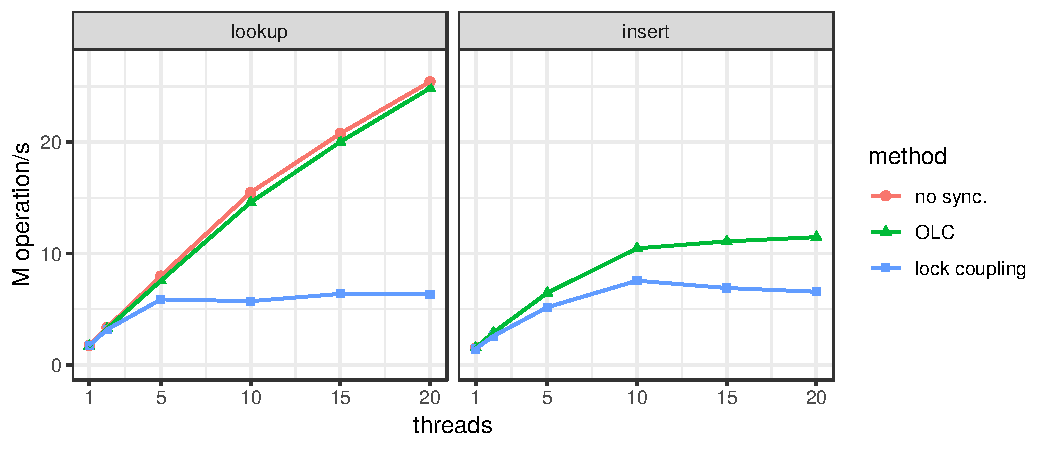
\includegraphics[width=\linewidth]{scale.pdf}
  \vspace{0.2cm}
  \caption{Scalability on 10-core system for B-tree operations (100M values).}
  \label{fig:scale}
\end{figure}

As Figure~\ref{fig:scale} shows, the results change dramatically once we use multiple threads.
For lookup, the scalability of OLC is near-linear up to 20 threads, even though the system has only 10 ``real cores''.
The OLC scalability for insert is also respectable (though not quite as linear because multi-threaded insertion approaches the memory bandwidth of our processor).
The figure also shows that the results of traditional lock coupling with read/write locks are significantly worse than OLC.
With 20 threads, lookup with OLC is 3.9$\times$ faster than traditional lock coupling.

\section{Summary}\label{sec:conc}

Optimistic Lock Coupling (OLC) is an effective synchronization method that combines the simplicity of traditional lock coupling with the superior scalability of lock-free approaches.
OLC is widely applicable and has already been successfully used to synchronize several data structures, including B-trees, binary search trees, and different trie variants.
These features make it highly attractive for modern database systems as well as performance-critical systems software in general.

\begin{thebibliography}{10}

\bibitem{DBLP:conf/spaa/BalmauGHZ16}
O.~Balmau, R.~Guerraoui, M.~Herlihy, and I.~Zablotchi.
\newblock Fast and robust memory reclamation for concurrent data structures.
\newblock In {\em SPAA}, 2016.

\bibitem{DBLP:journals/acta/BayerS77}
R.~Bayer and M.~Schkolnick.
\newblock Concurrency of operations on {B}-trees.
\newblock {\em Acta Informatica}, 9, 1977.

\bibitem{hot}
R.~Binna, E.~Zangerle, M.~Pichl, G.~Specht, and V.~Leis.
\newblock {HOT}: A height optimized trie index for main-memory database
  systems.
\newblock In {\em SIGMOD}, 2018.

\bibitem{DBLP:conf/ppopp/BronsonCCO10}
N.~G. Bronson, J.~Casper, H.~Chafi, and K.~Olukotun.
\newblock A practical concurrent binary search tree.
\newblock In {\em PPOPP}, 2010.

\bibitem{DBLP:conf/vldb/ChaHKK01}
S.~K. Cha, S.~Hwang, K.~Kim, and K.~Kwon.
\newblock Cache-conscious concurrency control of main-memory indexes on
  shared-memory multiprocessor systems.
\newblock In {\em VLDB}, 2001.

\bibitem{intel}
I.~Cutress.
\newblock {Intel} goes for 48-cores: {Cascade-AP} with multi-chip package
  coming soon.
\newblock
  \url{https://www.anandtech.com/show/13535/intel-goes-for-48cores-cascade-ap},
  2018 (accessed January, 2019).

\bibitem{DBLP:conf/cidr/FaleiroA17}
J.~M. Faleiro and D.~J. Abadi.
\newblock Latch-free synchronization in database systems: Silver bullet or
  fool's gold?
\newblock In {\em CIDR}, 2017.

\bibitem{DBLP:journals/ftdb/Graefe11}
G.~Graefe.
\newblock Modern {B}-tree techniques.
\newblock {\em Foundations and Trends in Databases}, 3(4), 2011.

\bibitem{DBLP:conf/hpca/KarnagelDRLLSL14}
T.~Karnagel, R.~Dementiev, R.~Rajwar, K.~Lai, T.~Legler, B.~Schlegel, and
  W.~Lehner.
\newblock Improving in-memory database index performance with
  {Intel}\({}^{\mbox{{\textregistered}}}\) transactional synchronization
  extensions.
\newblock In {\em HPCA}, 2014.

\bibitem{DBLP:journals/tods/LehmanY81}
P.~L. Lehman and S.~B. Yao.
\newblock Efficient locking for concurrent operations on {B}-trees.
\newblock {\em {ACM} Trans. Database Syst.}, 6(4), 1981.

\bibitem{leanstore}
V.~Leis, M.~Haubenschild, A.~Kemper, and T.~Neumann.
\newblock Leanstore: In-memory data management beyond main memory.
\newblock In {\em ICDE}, 2018.

\bibitem{art}
V.~Leis, A.~Kemper, and T.~Neumann.
\newblock The adaptive radix tree: {ARTful} indexing for main-memory databases.
\newblock In {\em ICDE}, 2013.

\bibitem{htmtkde}
V.~Leis, A.~Kemper, and T.~Neumann.
\newblock Scaling {HTM}-supported database transactions to many cores.
\newblock {\em {IEEE} Trans. Knowl. Data Eng.}, 28(2), 2016.

\bibitem{artsync}
V.~Leis, F.~Scheibner, A.~Kemper, and T.~Neumann.
\newblock The {ART} of practical synchronization.
\newblock In {\em DaMoN}, 2016.

\bibitem{DBLP:conf/icde/LevandoskiLS13a}
J.~J. Levandoski, D.~B. Lomet, and S.~Sengupta.
\newblock The {Bw}-tree: A {B}-tree for new hardware platforms.
\newblock In {\em ICDE}, 2013.

\bibitem{DBLP:journals/pvldb/MakreshanskiLS15}
D.~Makreshanski, J.~J. Levandoski, and R.~Stutsman.
\newblock To lock, swap, or elide: On the interplay of hardware transactional
  memory and lock-free indexing.
\newblock {\em {PVLDB}}, 8(11), 2015.

\bibitem{DBLP:dblp_conf/eurosys/MaoKM12}
Y.~Mao, E.~Kohler, and R.~T. Morris.
\newblock Cache craftiness for fast multicore key-value storage.
\newblock In {\em EuroSys}, 2012.

\bibitem{DBLP:journals/tpds/Michael04}
M.~M. Michael.
\newblock Hazard pointers: Safe memory reclamation for lock-free objects.
\newblock {\em {IEEE} Trans. Parallel Distrib. Syst.}, 15(6), 2004.

\bibitem{DBLP:journals/jacm/ShalevS06}
O.~Shalev and N.~Shavit.
\newblock Split-ordered lists: Lock-free extensible hash tables.
\newblock {\em J. {ACM}}, 53(3), 2006.

\bibitem{amd}
A.~Shilov.
\newblock {AMD} previews {EPYC} ‘{Rome}’ processor: Up to 64 {Zen} 2 cores.
\newblock
  \url{https://www.anandtech.com/show/13561/amd-previews-epyc-rome-processor-up-to-64-zen-2-cores},
  2018 (accessed January, 2019).

\bibitem{DBLP:conf/sosp/TuZKLM13}
S.~Tu, W.~Zheng, E.~Kohler, B.~Liskov, and S.~Madden.
\newblock Speedy transactions in multicore in-memory databases.
\newblock In {\em SOSP}, 2013.

\bibitem{buzzword}
Z.~Wang, A.~Pavlo, H.~Lim, V.~Leis, H.~Zhang, M.~Kaminsky, and D.~Andersen.
\newblock Building a {Bw}-tree takes more than just buzz words.
\newblock In {\em SIGMOD}, 2018.

\end{thebibliography}


%\bibliographystyle{abbrv}
%\bibliography{main}

\end{document}

\end{article}
\begin{article}
{Generative Explanation for Graph Neural Network: Methods and Evaluation}
{Rex Ying}
\pdfminorversion=5
\documentclass[11pt]{article}
\usepackage{deauthor,times,graphicx,caption,microtype}
\usepackage{hyperref}
\usepackage{listings}
\usepackage{booktabs}

\begin{document}

\title{Optimistic Lock Coupling: A Scalable and Efficient General-Purpose Synchronization Method}

\author{Viktor Leis, Michael Haubenschild\raisebox{0.9ex}{$\ast$}, Thomas Neumann\\ Technische Universit{\"a}t M{\"u}nchen \hspace{0.7cm} Tableau Software\raisebox{0.9ex}{$\ast$} \\ {\{leis,neumann\}{@}in.tum.de} \hspace{0.7cm} {mhaubenschild{@}tableau.com\raisebox{0.9ex}{$\ast$}}}

\maketitle

\begin{abstract}
As the number of cores on commodity processors continues to increase, scalability becomes more and more crucial for overall performance.
Scalable and efficient concurrent data structures are particularly important, as these are often the building blocks of parallel algorithms.
Unfortunately, traditional synchronization techniques based on fine-grained locking have been shown to be unscalable on modern multi-core CPUs.
Lock-free data structures, on the other hand, are extremely difficult to design and often incur significant overhead.

In this work, we make the case for Optimistic Lock Coupling as a practical alternative to both traditional locking and the lock-free approach.
We show that Optimistic Lock Coupling is highly scalable and almost as simple to implement as traditional lock coupling.
Another important advantage is that it is easily applicable to most tree-like data structures.
We therefore argue that Optimistic Lock Coupling, rather than a complex and error-prone custom synchronization protocol, should be the default choice for performance-critical data structures.
\end{abstract}

\section{Introduction}

% more and more cores
Today, Intel's commodity server processors have up to 28 cores and its upcoming microarchitecture will have up to 48 cores per socket~\cite{intel}.
Similarly, AMD currently stands at 32 cores and this number is expected to double in the next generation~\cite{amd}.
Since both platforms support simultaneous multithreading (also known as hyperthreading), affordable commodity servers (with up to two sockets) will soon routinely have between 100 and 200 hardware threads.

% data structure scalability is important
With such a high degree of hardware parallelism, efficient data processing crucially depends on how well concurrent data structures scale.
Internally, database systems use a plethora of data structures like table heaps, internal work queues, and, most importantly, index structures.
Any of these can easily become a scalability (and therefore overall performance) bottleneck on many-core CPUs.

% traditional synchronization: fine-grained locks, slow, cache invalidation
Traditionally, database systems synchronize internal data structures using fine-grained reader/writer locks\footnote{In this work, we focus on data structure synchronization rather than high-level transaction semantics and therefore use the term {\em lock} for what would typically be called {\em latch} in the database literature. We thus follow common computer science (rather than database) terminology.}.
Unfortunately, while fine-grained locking makes lock contention unlikely, it still results in bad scalability because lock acquisition and release require writing to shared memory.
Due to the way cache coherency is implemented on modern multi-core CPUs, these writes cause additional cache misses\footnote{The cache coherency protocol ensures that all copies of a cache line on other cores are invalidated before the write can proceed.} and the cache line containing the lock's internal data becomes a point of physical contention.
As a result, any frequently-accessed lock (e.g., the lock of the root node of a B-tree) severely limits scalability.

% lock-free bw-tree: no more latches, but indirections, extremely complex
Lock-free data structures like the Bw-tree~\cite{DBLP:conf/icde/LevandoskiLS13a} (a lock-free B-tree variant) or the Split-Ordered List~\cite{DBLP:journals/jacm/ShalevS06} (a lock-free hash table) do not acquire any locks and therefore generally scale much better than locking-based approaches (in particular for read-mostly workloads).
However, lock-free synchronization has other downsides:
First, it is very difficult and results in extremely complex and error-prone code (when compared to locking).
Second, because the functionality of atomic primitives provided by the hardware (e.g., atomically compare-and-swap 8 bytes) is limited, complex operations require additional indirections within the data structure.
For example, the Bw-tree requires an indirection table and the Split-Ordered List requires ``dummy nodes'', resulting in overhead due to additional cache misses.

% OLC for the win
In this paper we make the case for {\em Optimistic Lock Coupling (OLC)}, a synchronization method that combines some of the best properties of lock-based and lock-free synchronization.
OLC utilizes a special lock type that can be used in two modes:
The first mode is similar to a traditional mutex and excludes other threads by physically acquiring the underlying lock.
In the second mode, reads can proceed optimistically by validating a version counter that is embedded in the lock (similar to optimistic concurrency control).
The first mode is typically used by writers and the second mode by readers.
Besides this special lock type, OLC is based on the observation that optimistic lock validations can be interleaved/coupled---similar to the pair-wise interleaved lock acquisition of traditional lock coupling.
Hence, the name Optimistic Lock Coupling.

OLC has a number of desirable features:
\begin{itemize}
\item By reducing the number of writes to shared memory locations and thereby avoiding cache invalidations, it {\bf scales well} for most workloads.
\item In comparison to unsynchronized code, it requires few additional CPU instructions making it {\bf efficient}.
\item OLC is {\bf widely applicable} to different data structures. It has already been successfully used for synchronizing binary search trees~\cite{DBLP:conf/ppopp/BronsonCCO10}, tries~\cite{artsync}, trie/B-tree hybrids~\cite{DBLP:dblp_conf/eurosys/MaoKM12}, and B-trees~\cite{buzzword}.
\item In comparison to the lock-free paradigm, it is also {\bf easy to use} and requires few modifications to existing, single-threaded data structures.
\end{itemize}
Despite these positive features and its simplicity, OLC is not yet widely known.
The goal of this paper is therefore to popularize this simple idea and to make a case for it.
We argue that OLC deserves to be widely known.
It is a good default synchronization paradigm---more complex, data structure-specific protocols are seldom beneficial.

The rest of the paper is organized as follows.
Section~\ref{sec:related} discusses related work, tracing the history of OLC and its underlying ideas in the literature.
The core of the paper is Section~\ref{sec:olc}, which describes the ideas behind OLC and how it can be used to synchronize complex data structures.
In Section~\ref{sec:evaluation} we experimentally show that OLC has low overhead and scales well when used to synchronize an in-memory B-tree.
We summarize the paper in Section~\ref{sec:conc}.

\newpage
\section{Related Work}\label{sec:related}

Lock coupling has been proposed as a method for allowing concurrent operations on B-trees in 1977~\cite{DBLP:journals/acta/BayerS77}.
This traditional and still widely-used method, described in detail in Graefe's B-tree survey~\cite{DBLP:journals/ftdb/Graefe11}, is also called ``latch coupling'', ``hand-over-hand locking'', and ``crabbing''.
Because at most two locks are held at-a-time during tree traversal, this technique seemingly allows for a high degree of parallelism---in particular if read/write locks are used to enable inner nodes to be locked in shared mode.
However, as we show in Section~\ref{sec:evaluation}, on modern hardware lock acquisition (even in shared mode) results in suboptimal scalability.

An early alternative from 1981 is a B-tree variant called B-link tree~\cite{DBLP:journals/tods/LehmanY81}, which only holds a single lock at a time.
It is based on the observation that between the release of the parent lock and the acquisition of the child lock, the only ``dangerous'' thing that could have happened is the split of a child node (assuming one does not implement merge operations).
Thus, when a split happens, the key being searched might end up on a neighboring node to the right of the current child node.
A B-link tree traversal therefore detects this condition and, if needed, transparently proceeds to the neighboring node.
Releasing the parent lock early is highly beneficial when the child node needs to be fetched from disk.
For in-memory workloads, however, the B-link tree has the same scalability issues as lock coupling (it acquires just as many locks).

The next major advance, Optimistic Latch-Free Index Traversal (OLFIT)~\cite{DBLP:conf/vldb/ChaHKK01}, was proposed in 2001.
OLFIT introduced the idea of a combined lock/update counter, which we call {\em optimistic lock}. % , for lack of a better name,
Based on these per-node optimistic locks and the synchronization protocol of the B-link tree, OLFIT finally achieves good scalability on parallel processors.
The OLFIT protocol is fairly complex, as it requires both the non-trivial B-link protocol and optimistic locks.
Furthermore, like the B-link tree protocol, it does not support merging nodes, and is specific to B-trees (cannot easily be applied to other data structures).

In the following two decades, the growth of main-memory capacity led to much research into other data structures besides the venerable B-tree.
Particularly relevant for our discussion is Bronson et al.'s~\cite{DBLP:conf/ppopp/BronsonCCO10} concurrent binary search tree, which is based on optimistic version validation and has a sophisticated, data structure-specific synchronization protocol.
To the best of our knowledge, this 2010 paper is the first that, as part of its protocol, interleaves version validation across nodes---rather than validating each node separately like OLFIT.
In that paper, this idea is called ``hand-over-hand, optimistic validation'', while we prefer the term Optimistic Lock Coupling to highlight the close resemblance to traditional lock coupling.
Similarly, Mao et al.'s~\cite{DBLP:dblp_conf/eurosys/MaoKM12} Masstree (a concurrent hybrid trie/B-tree) is also based on the same ideas, but again uses them as part of a more complex protocol.

The Adaptive Radix Tree (ART)~\cite{art} is another recent in-memory data structure, which we proposed in 2013.
In contrast to the two data structures just mentioned, it was originally designed with single-threaded performance in mind without supporting concurrency.
To add support for concurrency, we initially started designing a custom protocol called Read-Optimized Write Exclusion (ROWEX)~\cite{artsync}, which turned out to be non-trivial and requires modifications of the underlying data structure\footnote{Note that ROWEX is already easier to apply to existing data structures than the lock-free approach. The difficulty depends on the data structure. Applying ROWEX is hard for B-trees with sorted keys and fairly easy for copy-on-write data structures like the Height Optimized Trie~\cite{hot}---with ART being somewhere in the middle.}.
However, fairly late in the project, we also realized, that OLC {\em alone} (rather than as part of a more complex protocol) is sufficient to synchronize ART.
No other changes to the data structure were necessary.
Both approaches were published and experimentally evaluated in a followup paper~\cite{artsync}, which shows that, despite its simplicity, OLC is efficient, scalable, and generally outperforms ROWEX.

Similar results were recently published regarding B-trees~\cite{buzzword}.
In this experimental study a simple OLC-based synchronization outperformed the Bw-tree~\cite{DBLP:conf/icde/LevandoskiLS13a}, a complex lock-free synchronization approach.
Another recent paper shows that for write-intensive workloads, locking often performs better than lock-free synchronization~\cite{DBLP:conf/cidr/FaleiroA17}.
These experiences indicate that OLC is a general-purpose synchronization paradigm and motivate the current paper.

%foster b-tree\cite{DBLP:journals/tods/GraefeKK12}
%Shasha theory~\cite{DBLP:journals/tods/ShashaG88}

\section{Optimistic Lock Coupling}\label{sec:olc}

% locks suck
The standard technique for inter-thread synchronization is mutual exclusion using fine-grained locks.
In a B-tree, for example, every node usually has its own associated lock, which is acquired before accessing that node.
The problem of locking on modern multi- and many-core processors is that lock acquisition and release require writing to the shared memory location that implements the lock.
This write causes exclusive ownership of the underlying cache line and invalidates copies of it on all other processor cores.
For hierarchical, tree-like data structures, the lock of the root node becomes a point of physical contention---even in read-only workloads and even when read/write locks are used.
Depending on the specific data structure, number of cores, cache coherency protocol implementation, cache topology, whether Non-Uniform Memory Access (NUMA) is used, locking can even result in multi-threaded performance that is worse than single-threaded execution.

% in b-trees this happens very much
The inherent pessimism of locking is particularly unfortunate for B-trees:
Despite the fact that logical modifications of the root node are very infrequent, every B-tree operation must lock the root node during tree traversal\footnote{To a lesser extent this obviously applies to all inner nodes, not just the root.}.
Even the vast majority of update operations (with the exception of splits and merges), only modify a single leaf node.
These observations indicate that a more optimistic approach, which does not require locking inner nodes, would be very beneficial for B-trees.

\subsection{Optimistic Locks}

% optimism to the rescue
As the name indicates, optimistic locks try to solve the scalability issues of traditional locks using an optimistic approach.
Instead of always physically acquiring locks, even for nodes that are unlikely to be modified simultaneously, after-the-fact validation is used to detect conflicts.
This is done by augmenting each lock with a version/update counter that is incremented on every modification.
Using this version counter, readers can optimistically proceed before validating that the version did not change to ensure that the read was safe.
If validation fails, the operation is restarted.

% details on opt locks
Using optimistic locks, a read-only node access (i.e., the majority of all operations in a B-tree) does not acquire the lock and does not increment the version counter.
Instead, it performs the following steps:
\begin{enumerate}
\item read lock version (restart if lock is not free)
\item access node
\item read the version again and validate that it has not changed in the meantime
\end{enumerate}
If the last step (the validation) fails, the operation has to be restarted.
Write operations, on the other hand, are more similar to traditional locking:
\begin{enumerate}
\item acquire lock (wait if necessary)
\item access/write to node
\item increment version and unlock node
\end{enumerate}
Writes can therefore protect a node from other writes.

% similar to locks
As we observed in an earlier paper~\cite{artsync}, because of similar semantics, optimistic locks can be hidden behind an API very similar to traditional read/write locks.
Both approaches have an exclusive lock mode, and acquiring a traditional lock in shared mode is analogous to optimistic version validation.
Furthermore, like with some implementations of traditional read/write locks, optimistic locks allow upgrading a shared lock to an exclusive lock.
Lock upgrades are, for example, used to avoid most B-tree update operations from having to lock inner nodes.
In our experience, the close resemblance of optimistic and traditional locks simplifies the reasoning about optimistic locks;
one can apply similar thinking as in traditional lock-based protocols.

\subsection{Lock Coupling with Optimistic Locks}

\begin{figure}
  \centering
  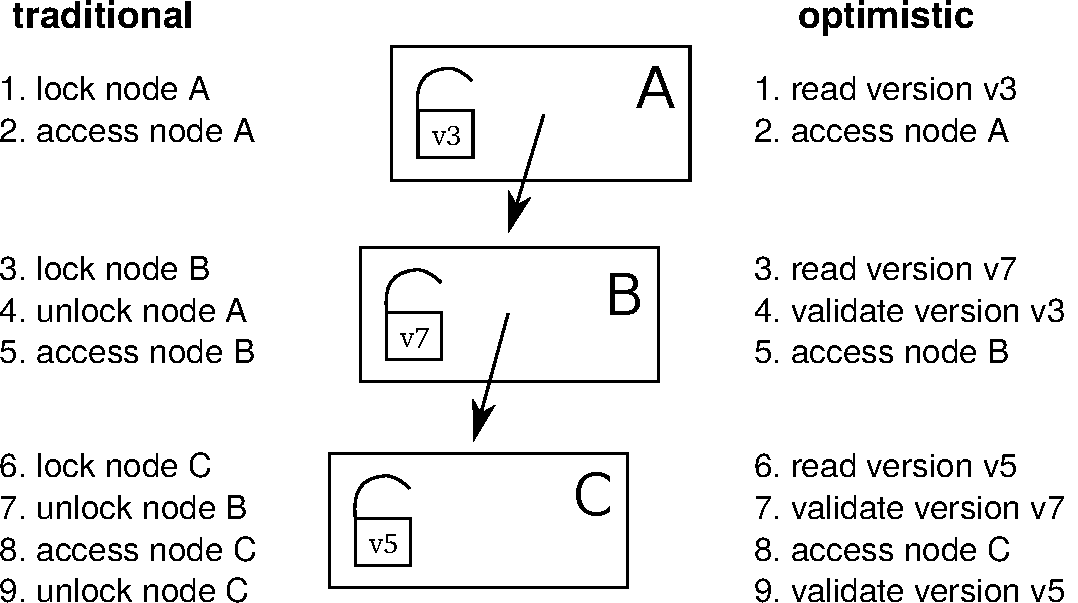
\includegraphics[width=0.65\linewidth]{olcall.pdf}
  \vspace{0.2cm}
  \caption{Comparison of a lookup operation in a 3-level tree using traditional lock coupling (left-hand side) vs.~optimistic lock coupling (right-hand side).}
  \label{fig:olc}
\end{figure}

The traditional and most common lock-based synchronization protocol for B-trees is lock coupling, which interleaves lock acquisitions while holding at most two locks at a time.
If, as we observed earlier, optimistic locks have similar semantics as traditional locks, it is natural to ask whether lock coupling can be combined with optimistic locks.
And indeed the answer is yes: One can almost mechanically translate traditional lock coupling code to optimistic lock coupling code.
This is illustrated in Figure~\ref{fig:olc}, which compares the traversal in a tree of height 3 using traditional and optimistic locks.
As the figure shows, the main difference is that locking is translated to reading the version and that unlocking becomes validation of the previously read version.
This simple change provides efficient lock-free tree traversal without the need to design a complex synchronization protocol.

It is important to emphasize the conceptual simplicity of OLC in comparison to data structures that use custom protocols like the Bw-tree~\cite{DBLP:conf/icde/LevandoskiLS13a}.
To implement lock-free access, the Bw-tree requires an indirection table, delta nodes, complex splitting and merging logic, retry logic, etc.
OLC, on the other hand, can directly be applied to B-trees mostly by adding the appropriate optimistic locking code and without modifying the node layout itself.
Therefore, OpenBw-Tree, an open source implementation of the Bw-tree, requires an order of magnitude more code than a B-tree based on OLC\footnote{Both implementations are available on GitHub: \url{https://github.com/wangziqi2016/index-microbench}}.
Given how difficult it is to develop, validate, and debug lock-free code, simplicity is obviously a major advantage.

\subsection{Correctness Aspects}

\begin{figure}
  % \centering
  %[basicstyle=\normalsize\ttfamily,showstringspaces=false,columns=fullflexible,breaklines=false,breakatwhitespace=true,numbers=none,numberstyle=\small,style=C,keepspaces=true]
\begin{lstlisting}[basicstyle=\ttfamily,language=C++,numbers=left,numberstyle=\small]
std::atomic<BTreeNode*> root;

// search for key in B+tree, returns payload in resultOut
bool lookup(Key key, Value& resultOut) {
   BTreeNode* node = root.load();
   uint64_t nodeVersion = node->readLockOrRestart();
   if (node != root.load()) // make sure the root is still the root
      restart();

   BTreeInner<Key>* parent = nullptr;
   uint64_t parentVersion = 0;

   while (node->isInner()) {
      auto inner = (BTreeInner*)node;

      // unlock parent and make current node the parent
      if (parent)
         parent->readUnlockOrRestart(parentVersion);
      parent = inner;
      parentVersion = nodeVersion;

      // search for next node
      node = inner->findChild(key);
      // validate 'inner' to ensure that 'node' pointer is valid
      inner->checkOrRestart(nodeVersion);
      // now it safe to dereference 'node' pointer (read its version)
      nodeVersion = node->readLockOrRestart();
   }

   // search in leaf and retrieve payload
   auto leaf = (BTreeLeaf*)node;
   bool success = leaf->findValue(key, resultOut);

   // unlock everything
   if (parent)
      parent->readUnlockOrRestart(parentVersion);
   node->readUnlockOrRestart(nodeVersion);

   return success;
}
\end{lstlisting}
  \vspace{0.2cm}
  \caption{B-tree lookup code using OLC. For simplicity, the restart logic is not shown.}
  \label{fig:lookup}
\end{figure}

So far, we have introduced the high-level ideas behind OLC and have stressed its similarity to traditional lock coupling.
Let us now discuss some cases where the close similarity between lock coupling and OLC breaks down.
To make this more concrete, we show the B-tree lookup code in Figure~\ref{fig:lookup}.
In the code, \texttt{readLockOrRestart} reads the lock version and \texttt{readUnlockOrRestart} validates that the read was correct.

One issue with OLC is that any pointer speculatively read from a node may point to invalid memory (if that node is modified concurrently).
Dereferencing such a pointer (e.g., to read its optimistic lock), may cause a segmentation fault or undefined behavior.
In the code shown in Figure~\ref{fig:lookup}, this problem is prevented by the extra check in line 25, which ensures that the read from the node containing the pointer was correct.
Without this additional validation, the code would in line 27 dereference the pointer speculatively read in line 23.
Note that the implementation of \texttt{checkOrRestart} is actually identical to \texttt{readUnlockOrRestart}.
We chose to give it a different name to highlight the fact that this extra check would not be necessary with read/write locks.

Another potential issue with optimistic locks is code that does not terminate.
Code that speculatively accesses a node, like an intra-node binary search, should be written in a way such that it always terminates---even in the presence of concurrent writes.
Otherwise, the validation code that detects the concurrent write will never run.
The binary search of a B-tree, for example, needs to be written in such a way that each comparison makes progress.
For some data structures that do not require loops in the traversal code (like ART) termination is trivially true.

\subsection{Implementation Details}

% implementation, efficiency
To implement an optimistic lock, one can combine the lock and the version counter into a single 64-bit\footnote{Even after subtracting one bit for the lock status, a back-of-the-envelope calculation can show that 63 bits are large enough to never overflow in practice.} word~\cite{artsync}.
A typical read operation will therefore merely consist of reading this version counter atomically.
In C++11 this can be implemented using the \texttt{std::atomic} type.

On x86, atomic reads are cheap because of x86's strong memory order guarantees.
No memory fences are required for sequentially-consistent loads, which are translated (by both GCC and clang) into standard \texttt{MOV} instructions.
Hence, the only effect of \texttt{std::atomic} for loads is preventing instruction re-ordering.
This makes version access and validation cheap.
Acquiring and releasing an optimistic lock in exclusive mode has comparable cost to a traditional lock:
A fairly expensive sequentially-consistent store is needed for acquiring a lock, while a standard \texttt{MOV} suffices for releasing it.
A simple sinlock-based implementation of optimistic locks can be found in the appendix of an earlier paper~\cite{artsync}.

OLC code must be able to handle restarts since validation or lock upgrade can fail due to concurrent writers.
Restarts can easily be implemented by wrapping the data structure operation in a loop (for simplicity not shown in Figure~\ref{fig:lookup}).
Such a loop also enables limiting the number of optimistic retry operations and falling back to pessimistic locking in cases of very heavy contention.
The ability to fall back to traditional locking is a major advantage of OLC in terms of robustness over lock-free approaches, which do not have this option.

In addition to the optimistic shared mode and the exclusive mode, optimistic locks also support a ``shared pessimistic'' mode, which physically acquires the lock in shared mode (allowing multiple concurrent readers but no writers).
This mode is useful for table (or range) scans that touch many tuples on a leaf page (which would otherwise easily abort).
Finally, let us mention that large range scans and table scans, should be broken up into several per-node traversals as is done in the LeanStore~\cite{leanstore} system.

Like all lock-free data structures, but unlike traditional locking and Hardware Transactional Memory~\cite{DBLP:conf/hpca/KarnagelDRLLSL14,DBLP:journals/pvldb/MakreshanskiLS15,htmtkde}, OLC requires care when deleting (and reusing) nodes.
The reason is that a deleting thread can never be sure that a node can be reclaimed because other threads might still be optimistically reading from that node.
Therefore, standard solutions like epoch-based reclamation~\cite{DBLP:conf/sosp/TuZKLM13}, hazard pointers~\cite{DBLP:journals/tpds/Michael04}, or optimized hazard pointers~\cite{DBLP:conf/spaa/BalmauGHZ16} need to be used.
These memory reclamation techniques are, however, largely orthogonal to the synchronization protocol itself.

%-lock-free is not a strong guarantee

\newpage
\section{Evaluation}\label{sec:evaluation}

Let us now experimentally evaluate the overhead and scalability of OLC.
For the experiments, we use an in-memory B+tree implemented in C++11 using templates, which is configured to use nodes of 4096 bytes, random 8 byte keys, and 8 byte payloads.
Based on this B-tree, we compare the following synchronization approaches:
\begin{itemize}
\item an OLC implementation\footnote{An almost identical OLC implementation is available on github: \url{https://github.com/wangziqi2016/index-microbench/tree/master/BTreeOLC}}
\item a variant based on traditional lock coupling and read/write locks
\item the unsynchronized B-tree, which obviously is only correct for read-only workloads but allows measuring the overhead of synchronization
\end{itemize}
Note that earlier work has compared the OLC implementation with a Bw-tree implementation~\cite{buzzword} and other state-of-the-art in-memory index structures.

We use a Haswell EP system with an Intel Xeon E5-2687W v3 CPU, which has 10 cores (20 ``Hyper-Threads'') and 25~MB of L3 cache.
The system is running Ubuntu 18.10 and we use GCC 8.2.0 to compile our code.
The CPU counters are obtained using the Linux perf API\footnote{We use the following convenience wrapper: \url{https://github.com/viktorleis/perfevent}}.

\begin{table}
  \caption{Performance and CPU counters for lookup and insert operations in a B-tree with 100M keys. We perform 100M operations and normalize the CPU counters by that number.}
  \label{tab:overhead}
  \centering
  \begin{tabular}{lrrrrrrr}\toprule
                    &         &        &        & instruc-  & L1     & L3     & branch \\
                    & threads & M op/s & cycles & tions & misses & misses & misses \\\midrule
lookup (no sync.)   & 1       & 1.72   & 2028   & 283     & 39.1   & 14.9   & 16.1   \\
lookup (OLC)        & 1       & 1.65   & 2107   & 370     & 43.9   & 15.1   & 16.7   \\
lookup (lock coup.) & 1       & 1.72   & 2078   & 365     & 42.3   & 16.9   & 15.7   \\\midrule
insert (no sync.)   & 1       & 1.51   & 2286   & 530     & 59.8   & 31.1   & 17.3   \\
insert (OLC)        & 1       & 1.50   & 2303   & 629     & 61.2   & 31.1   & 16.5   \\
insert (lock coup.) & 1       & 1.41   & 2473   & 644     & 61.0   & 31.0   & 17.2   \\\midrule
lookup (no sync.)   & 10      & 15.48  & 2058   & 283     & 38.6   & 15.5   & 16.0   \\
lookup (OLC)        & 10      & 14.60  & 2187   & 370     & 43.8   & 15.8   & 16.8   \\
lookup (lock coup.) & 10      & 5.71   & 5591   & 379     & 54.2   & 17.0   & 14.8   \\\midrule
insert (no sync.)   & 10      & -      & -      & -       & -      & -      & -      \\
insert (OLC)        & 10      & 10.46  & 2940   & 656     & 62.0   & 32.5   & 16.8   \\
insert (lock coup.) & 10      & 7.55   & 4161   & 667     & 75.0   & 28.6   & 16.2   \\
    \bottomrule
\end{tabular}
\end{table}

Table~\ref{tab:overhead} compares the performance and CPU counters for lookup and insert operations in a B-tree with 100M keys.
With {\em single-threaded} execution, we observe that all three approaches have very similar performance.
Adding traditional or optimistic locks to unsynchronized B-tree code results in up to 30\% of additional instructions without affecting single-threaded performance much.

\begin{figure}
  \centering
  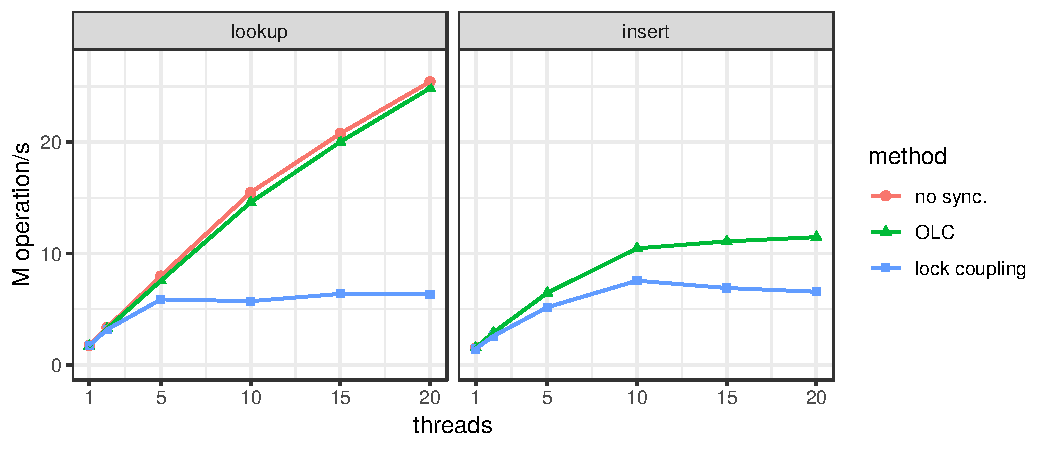
\includegraphics[width=\linewidth]{scale.pdf}
  \vspace{0.2cm}
  \caption{Scalability on 10-core system for B-tree operations (100M values).}
  \label{fig:scale}
\end{figure}

As Figure~\ref{fig:scale} shows, the results change dramatically once we use multiple threads.
For lookup, the scalability of OLC is near-linear up to 20 threads, even though the system has only 10 ``real cores''.
The OLC scalability for insert is also respectable (though not quite as linear because multi-threaded insertion approaches the memory bandwidth of our processor).
The figure also shows that the results of traditional lock coupling with read/write locks are significantly worse than OLC.
With 20 threads, lookup with OLC is 3.9$\times$ faster than traditional lock coupling.

\section{Summary}\label{sec:conc}

Optimistic Lock Coupling (OLC) is an effective synchronization method that combines the simplicity of traditional lock coupling with the superior scalability of lock-free approaches.
OLC is widely applicable and has already been successfully used to synchronize several data structures, including B-trees, binary search trees, and different trie variants.
These features make it highly attractive for modern database systems as well as performance-critical systems software in general.

\begin{thebibliography}{10}

\bibitem{DBLP:conf/spaa/BalmauGHZ16}
O.~Balmau, R.~Guerraoui, M.~Herlihy, and I.~Zablotchi.
\newblock Fast and robust memory reclamation for concurrent data structures.
\newblock In {\em SPAA}, 2016.

\bibitem{DBLP:journals/acta/BayerS77}
R.~Bayer and M.~Schkolnick.
\newblock Concurrency of operations on {B}-trees.
\newblock {\em Acta Informatica}, 9, 1977.

\bibitem{hot}
R.~Binna, E.~Zangerle, M.~Pichl, G.~Specht, and V.~Leis.
\newblock {HOT}: A height optimized trie index for main-memory database
  systems.
\newblock In {\em SIGMOD}, 2018.

\bibitem{DBLP:conf/ppopp/BronsonCCO10}
N.~G. Bronson, J.~Casper, H.~Chafi, and K.~Olukotun.
\newblock A practical concurrent binary search tree.
\newblock In {\em PPOPP}, 2010.

\bibitem{DBLP:conf/vldb/ChaHKK01}
S.~K. Cha, S.~Hwang, K.~Kim, and K.~Kwon.
\newblock Cache-conscious concurrency control of main-memory indexes on
  shared-memory multiprocessor systems.
\newblock In {\em VLDB}, 2001.

\bibitem{intel}
I.~Cutress.
\newblock {Intel} goes for 48-cores: {Cascade-AP} with multi-chip package
  coming soon.
\newblock
  \url{https://www.anandtech.com/show/13535/intel-goes-for-48cores-cascade-ap},
  2018 (accessed January, 2019).

\bibitem{DBLP:conf/cidr/FaleiroA17}
J.~M. Faleiro and D.~J. Abadi.
\newblock Latch-free synchronization in database systems: Silver bullet or
  fool's gold?
\newblock In {\em CIDR}, 2017.

\bibitem{DBLP:journals/ftdb/Graefe11}
G.~Graefe.
\newblock Modern {B}-tree techniques.
\newblock {\em Foundations and Trends in Databases}, 3(4), 2011.

\bibitem{DBLP:conf/hpca/KarnagelDRLLSL14}
T.~Karnagel, R.~Dementiev, R.~Rajwar, K.~Lai, T.~Legler, B.~Schlegel, and
  W.~Lehner.
\newblock Improving in-memory database index performance with
  {Intel}\({}^{\mbox{{\textregistered}}}\) transactional synchronization
  extensions.
\newblock In {\em HPCA}, 2014.

\bibitem{DBLP:journals/tods/LehmanY81}
P.~L. Lehman and S.~B. Yao.
\newblock Efficient locking for concurrent operations on {B}-trees.
\newblock {\em {ACM} Trans. Database Syst.}, 6(4), 1981.

\bibitem{leanstore}
V.~Leis, M.~Haubenschild, A.~Kemper, and T.~Neumann.
\newblock Leanstore: In-memory data management beyond main memory.
\newblock In {\em ICDE}, 2018.

\bibitem{art}
V.~Leis, A.~Kemper, and T.~Neumann.
\newblock The adaptive radix tree: {ARTful} indexing for main-memory databases.
\newblock In {\em ICDE}, 2013.

\bibitem{htmtkde}
V.~Leis, A.~Kemper, and T.~Neumann.
\newblock Scaling {HTM}-supported database transactions to many cores.
\newblock {\em {IEEE} Trans. Knowl. Data Eng.}, 28(2), 2016.

\bibitem{artsync}
V.~Leis, F.~Scheibner, A.~Kemper, and T.~Neumann.
\newblock The {ART} of practical synchronization.
\newblock In {\em DaMoN}, 2016.

\bibitem{DBLP:conf/icde/LevandoskiLS13a}
J.~J. Levandoski, D.~B. Lomet, and S.~Sengupta.
\newblock The {Bw}-tree: A {B}-tree for new hardware platforms.
\newblock In {\em ICDE}, 2013.

\bibitem{DBLP:journals/pvldb/MakreshanskiLS15}
D.~Makreshanski, J.~J. Levandoski, and R.~Stutsman.
\newblock To lock, swap, or elide: On the interplay of hardware transactional
  memory and lock-free indexing.
\newblock {\em {PVLDB}}, 8(11), 2015.

\bibitem{DBLP:dblp_conf/eurosys/MaoKM12}
Y.~Mao, E.~Kohler, and R.~T. Morris.
\newblock Cache craftiness for fast multicore key-value storage.
\newblock In {\em EuroSys}, 2012.

\bibitem{DBLP:journals/tpds/Michael04}
M.~M. Michael.
\newblock Hazard pointers: Safe memory reclamation for lock-free objects.
\newblock {\em {IEEE} Trans. Parallel Distrib. Syst.}, 15(6), 2004.

\bibitem{DBLP:journals/jacm/ShalevS06}
O.~Shalev and N.~Shavit.
\newblock Split-ordered lists: Lock-free extensible hash tables.
\newblock {\em J. {ACM}}, 53(3), 2006.

\bibitem{amd}
A.~Shilov.
\newblock {AMD} previews {EPYC} ‘{Rome}’ processor: Up to 64 {Zen} 2 cores.
\newblock
  \url{https://www.anandtech.com/show/13561/amd-previews-epyc-rome-processor-up-to-64-zen-2-cores},
  2018 (accessed January, 2019).

\bibitem{DBLP:conf/sosp/TuZKLM13}
S.~Tu, W.~Zheng, E.~Kohler, B.~Liskov, and S.~Madden.
\newblock Speedy transactions in multicore in-memory databases.
\newblock In {\em SOSP}, 2013.

\bibitem{buzzword}
Z.~Wang, A.~Pavlo, H.~Lim, V.~Leis, H.~Zhang, M.~Kaminsky, and D.~Andersen.
\newblock Building a {Bw}-tree takes more than just buzz words.
\newblock In {\em SIGMOD}, 2018.

\end{thebibliography}


%\bibliographystyle{abbrv}
%\bibliography{main}

\end{document}

\end{article}
\begin{article}
{Graph Contrastive Learning: An Odyssey towards Generalizable, Scalable and Principled Representation Learning on Graphs}
{Yan Han, Yuning You, Wenqing Zheng, Scott Hoang, Tianxin Wei, Majdi Hassan, Tianlong Chen, Ying Ding, Yang Shen, Zhangyang Wang}
\pdfminorversion=5
\documentclass[11pt]{article}
\usepackage{deauthor,times,graphicx,caption,microtype}
\usepackage{hyperref}
\usepackage{listings}
\usepackage{booktabs}

\begin{document}

\title{Optimistic Lock Coupling: A Scalable and Efficient General-Purpose Synchronization Method}

\author{Viktor Leis, Michael Haubenschild\raisebox{0.9ex}{$\ast$}, Thomas Neumann\\ Technische Universit{\"a}t M{\"u}nchen \hspace{0.7cm} Tableau Software\raisebox{0.9ex}{$\ast$} \\ {\{leis,neumann\}{@}in.tum.de} \hspace{0.7cm} {mhaubenschild{@}tableau.com\raisebox{0.9ex}{$\ast$}}}

\maketitle

\begin{abstract}
As the number of cores on commodity processors continues to increase, scalability becomes more and more crucial for overall performance.
Scalable and efficient concurrent data structures are particularly important, as these are often the building blocks of parallel algorithms.
Unfortunately, traditional synchronization techniques based on fine-grained locking have been shown to be unscalable on modern multi-core CPUs.
Lock-free data structures, on the other hand, are extremely difficult to design and often incur significant overhead.

In this work, we make the case for Optimistic Lock Coupling as a practical alternative to both traditional locking and the lock-free approach.
We show that Optimistic Lock Coupling is highly scalable and almost as simple to implement as traditional lock coupling.
Another important advantage is that it is easily applicable to most tree-like data structures.
We therefore argue that Optimistic Lock Coupling, rather than a complex and error-prone custom synchronization protocol, should be the default choice for performance-critical data structures.
\end{abstract}

\section{Introduction}

% more and more cores
Today, Intel's commodity server processors have up to 28 cores and its upcoming microarchitecture will have up to 48 cores per socket~\cite{intel}.
Similarly, AMD currently stands at 32 cores and this number is expected to double in the next generation~\cite{amd}.
Since both platforms support simultaneous multithreading (also known as hyperthreading), affordable commodity servers (with up to two sockets) will soon routinely have between 100 and 200 hardware threads.

% data structure scalability is important
With such a high degree of hardware parallelism, efficient data processing crucially depends on how well concurrent data structures scale.
Internally, database systems use a plethora of data structures like table heaps, internal work queues, and, most importantly, index structures.
Any of these can easily become a scalability (and therefore overall performance) bottleneck on many-core CPUs.

% traditional synchronization: fine-grained locks, slow, cache invalidation
Traditionally, database systems synchronize internal data structures using fine-grained reader/writer locks\footnote{In this work, we focus on data structure synchronization rather than high-level transaction semantics and therefore use the term {\em lock} for what would typically be called {\em latch} in the database literature. We thus follow common computer science (rather than database) terminology.}.
Unfortunately, while fine-grained locking makes lock contention unlikely, it still results in bad scalability because lock acquisition and release require writing to shared memory.
Due to the way cache coherency is implemented on modern multi-core CPUs, these writes cause additional cache misses\footnote{The cache coherency protocol ensures that all copies of a cache line on other cores are invalidated before the write can proceed.} and the cache line containing the lock's internal data becomes a point of physical contention.
As a result, any frequently-accessed lock (e.g., the lock of the root node of a B-tree) severely limits scalability.

% lock-free bw-tree: no more latches, but indirections, extremely complex
Lock-free data structures like the Bw-tree~\cite{DBLP:conf/icde/LevandoskiLS13a} (a lock-free B-tree variant) or the Split-Ordered List~\cite{DBLP:journals/jacm/ShalevS06} (a lock-free hash table) do not acquire any locks and therefore generally scale much better than locking-based approaches (in particular for read-mostly workloads).
However, lock-free synchronization has other downsides:
First, it is very difficult and results in extremely complex and error-prone code (when compared to locking).
Second, because the functionality of atomic primitives provided by the hardware (e.g., atomically compare-and-swap 8 bytes) is limited, complex operations require additional indirections within the data structure.
For example, the Bw-tree requires an indirection table and the Split-Ordered List requires ``dummy nodes'', resulting in overhead due to additional cache misses.

% OLC for the win
In this paper we make the case for {\em Optimistic Lock Coupling (OLC)}, a synchronization method that combines some of the best properties of lock-based and lock-free synchronization.
OLC utilizes a special lock type that can be used in two modes:
The first mode is similar to a traditional mutex and excludes other threads by physically acquiring the underlying lock.
In the second mode, reads can proceed optimistically by validating a version counter that is embedded in the lock (similar to optimistic concurrency control).
The first mode is typically used by writers and the second mode by readers.
Besides this special lock type, OLC is based on the observation that optimistic lock validations can be interleaved/coupled---similar to the pair-wise interleaved lock acquisition of traditional lock coupling.
Hence, the name Optimistic Lock Coupling.

OLC has a number of desirable features:
\begin{itemize}
\item By reducing the number of writes to shared memory locations and thereby avoiding cache invalidations, it {\bf scales well} for most workloads.
\item In comparison to unsynchronized code, it requires few additional CPU instructions making it {\bf efficient}.
\item OLC is {\bf widely applicable} to different data structures. It has already been successfully used for synchronizing binary search trees~\cite{DBLP:conf/ppopp/BronsonCCO10}, tries~\cite{artsync}, trie/B-tree hybrids~\cite{DBLP:dblp_conf/eurosys/MaoKM12}, and B-trees~\cite{buzzword}.
\item In comparison to the lock-free paradigm, it is also {\bf easy to use} and requires few modifications to existing, single-threaded data structures.
\end{itemize}
Despite these positive features and its simplicity, OLC is not yet widely known.
The goal of this paper is therefore to popularize this simple idea and to make a case for it.
We argue that OLC deserves to be widely known.
It is a good default synchronization paradigm---more complex, data structure-specific protocols are seldom beneficial.

The rest of the paper is organized as follows.
Section~\ref{sec:related} discusses related work, tracing the history of OLC and its underlying ideas in the literature.
The core of the paper is Section~\ref{sec:olc}, which describes the ideas behind OLC and how it can be used to synchronize complex data structures.
In Section~\ref{sec:evaluation} we experimentally show that OLC has low overhead and scales well when used to synchronize an in-memory B-tree.
We summarize the paper in Section~\ref{sec:conc}.

\newpage
\section{Related Work}\label{sec:related}

Lock coupling has been proposed as a method for allowing concurrent operations on B-trees in 1977~\cite{DBLP:journals/acta/BayerS77}.
This traditional and still widely-used method, described in detail in Graefe's B-tree survey~\cite{DBLP:journals/ftdb/Graefe11}, is also called ``latch coupling'', ``hand-over-hand locking'', and ``crabbing''.
Because at most two locks are held at-a-time during tree traversal, this technique seemingly allows for a high degree of parallelism---in particular if read/write locks are used to enable inner nodes to be locked in shared mode.
However, as we show in Section~\ref{sec:evaluation}, on modern hardware lock acquisition (even in shared mode) results in suboptimal scalability.

An early alternative from 1981 is a B-tree variant called B-link tree~\cite{DBLP:journals/tods/LehmanY81}, which only holds a single lock at a time.
It is based on the observation that between the release of the parent lock and the acquisition of the child lock, the only ``dangerous'' thing that could have happened is the split of a child node (assuming one does not implement merge operations).
Thus, when a split happens, the key being searched might end up on a neighboring node to the right of the current child node.
A B-link tree traversal therefore detects this condition and, if needed, transparently proceeds to the neighboring node.
Releasing the parent lock early is highly beneficial when the child node needs to be fetched from disk.
For in-memory workloads, however, the B-link tree has the same scalability issues as lock coupling (it acquires just as many locks).

The next major advance, Optimistic Latch-Free Index Traversal (OLFIT)~\cite{DBLP:conf/vldb/ChaHKK01}, was proposed in 2001.
OLFIT introduced the idea of a combined lock/update counter, which we call {\em optimistic lock}. % , for lack of a better name,
Based on these per-node optimistic locks and the synchronization protocol of the B-link tree, OLFIT finally achieves good scalability on parallel processors.
The OLFIT protocol is fairly complex, as it requires both the non-trivial B-link protocol and optimistic locks.
Furthermore, like the B-link tree protocol, it does not support merging nodes, and is specific to B-trees (cannot easily be applied to other data structures).

In the following two decades, the growth of main-memory capacity led to much research into other data structures besides the venerable B-tree.
Particularly relevant for our discussion is Bronson et al.'s~\cite{DBLP:conf/ppopp/BronsonCCO10} concurrent binary search tree, which is based on optimistic version validation and has a sophisticated, data structure-specific synchronization protocol.
To the best of our knowledge, this 2010 paper is the first that, as part of its protocol, interleaves version validation across nodes---rather than validating each node separately like OLFIT.
In that paper, this idea is called ``hand-over-hand, optimistic validation'', while we prefer the term Optimistic Lock Coupling to highlight the close resemblance to traditional lock coupling.
Similarly, Mao et al.'s~\cite{DBLP:dblp_conf/eurosys/MaoKM12} Masstree (a concurrent hybrid trie/B-tree) is also based on the same ideas, but again uses them as part of a more complex protocol.

The Adaptive Radix Tree (ART)~\cite{art} is another recent in-memory data structure, which we proposed in 2013.
In contrast to the two data structures just mentioned, it was originally designed with single-threaded performance in mind without supporting concurrency.
To add support for concurrency, we initially started designing a custom protocol called Read-Optimized Write Exclusion (ROWEX)~\cite{artsync}, which turned out to be non-trivial and requires modifications of the underlying data structure\footnote{Note that ROWEX is already easier to apply to existing data structures than the lock-free approach. The difficulty depends on the data structure. Applying ROWEX is hard for B-trees with sorted keys and fairly easy for copy-on-write data structures like the Height Optimized Trie~\cite{hot}---with ART being somewhere in the middle.}.
However, fairly late in the project, we also realized, that OLC {\em alone} (rather than as part of a more complex protocol) is sufficient to synchronize ART.
No other changes to the data structure were necessary.
Both approaches were published and experimentally evaluated in a followup paper~\cite{artsync}, which shows that, despite its simplicity, OLC is efficient, scalable, and generally outperforms ROWEX.

Similar results were recently published regarding B-trees~\cite{buzzword}.
In this experimental study a simple OLC-based synchronization outperformed the Bw-tree~\cite{DBLP:conf/icde/LevandoskiLS13a}, a complex lock-free synchronization approach.
Another recent paper shows that for write-intensive workloads, locking often performs better than lock-free synchronization~\cite{DBLP:conf/cidr/FaleiroA17}.
These experiences indicate that OLC is a general-purpose synchronization paradigm and motivate the current paper.

%foster b-tree\cite{DBLP:journals/tods/GraefeKK12}
%Shasha theory~\cite{DBLP:journals/tods/ShashaG88}

\section{Optimistic Lock Coupling}\label{sec:olc}

% locks suck
The standard technique for inter-thread synchronization is mutual exclusion using fine-grained locks.
In a B-tree, for example, every node usually has its own associated lock, which is acquired before accessing that node.
The problem of locking on modern multi- and many-core processors is that lock acquisition and release require writing to the shared memory location that implements the lock.
This write causes exclusive ownership of the underlying cache line and invalidates copies of it on all other processor cores.
For hierarchical, tree-like data structures, the lock of the root node becomes a point of physical contention---even in read-only workloads and even when read/write locks are used.
Depending on the specific data structure, number of cores, cache coherency protocol implementation, cache topology, whether Non-Uniform Memory Access (NUMA) is used, locking can even result in multi-threaded performance that is worse than single-threaded execution.

% in b-trees this happens very much
The inherent pessimism of locking is particularly unfortunate for B-trees:
Despite the fact that logical modifications of the root node are very infrequent, every B-tree operation must lock the root node during tree traversal\footnote{To a lesser extent this obviously applies to all inner nodes, not just the root.}.
Even the vast majority of update operations (with the exception of splits and merges), only modify a single leaf node.
These observations indicate that a more optimistic approach, which does not require locking inner nodes, would be very beneficial for B-trees.

\subsection{Optimistic Locks}

% optimism to the rescue
As the name indicates, optimistic locks try to solve the scalability issues of traditional locks using an optimistic approach.
Instead of always physically acquiring locks, even for nodes that are unlikely to be modified simultaneously, after-the-fact validation is used to detect conflicts.
This is done by augmenting each lock with a version/update counter that is incremented on every modification.
Using this version counter, readers can optimistically proceed before validating that the version did not change to ensure that the read was safe.
If validation fails, the operation is restarted.

% details on opt locks
Using optimistic locks, a read-only node access (i.e., the majority of all operations in a B-tree) does not acquire the lock and does not increment the version counter.
Instead, it performs the following steps:
\begin{enumerate}
\item read lock version (restart if lock is not free)
\item access node
\item read the version again and validate that it has not changed in the meantime
\end{enumerate}
If the last step (the validation) fails, the operation has to be restarted.
Write operations, on the other hand, are more similar to traditional locking:
\begin{enumerate}
\item acquire lock (wait if necessary)
\item access/write to node
\item increment version and unlock node
\end{enumerate}
Writes can therefore protect a node from other writes.

% similar to locks
As we observed in an earlier paper~\cite{artsync}, because of similar semantics, optimistic locks can be hidden behind an API very similar to traditional read/write locks.
Both approaches have an exclusive lock mode, and acquiring a traditional lock in shared mode is analogous to optimistic version validation.
Furthermore, like with some implementations of traditional read/write locks, optimistic locks allow upgrading a shared lock to an exclusive lock.
Lock upgrades are, for example, used to avoid most B-tree update operations from having to lock inner nodes.
In our experience, the close resemblance of optimistic and traditional locks simplifies the reasoning about optimistic locks;
one can apply similar thinking as in traditional lock-based protocols.

\subsection{Lock Coupling with Optimistic Locks}

\begin{figure}
  \centering
  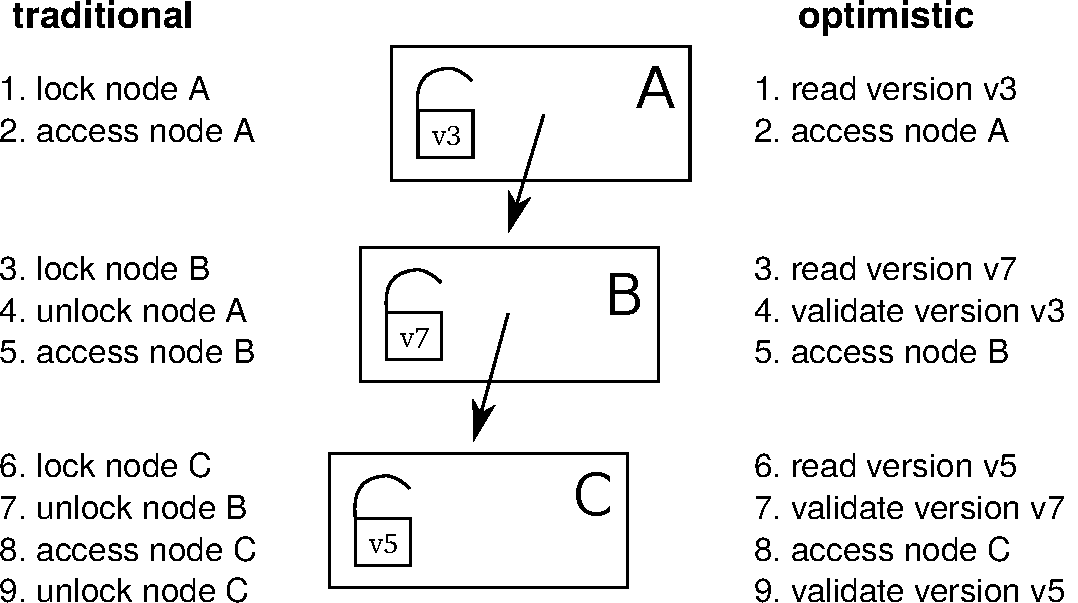
\includegraphics[width=0.65\linewidth]{olcall.pdf}
  \vspace{0.2cm}
  \caption{Comparison of a lookup operation in a 3-level tree using traditional lock coupling (left-hand side) vs.~optimistic lock coupling (right-hand side).}
  \label{fig:olc}
\end{figure}

The traditional and most common lock-based synchronization protocol for B-trees is lock coupling, which interleaves lock acquisitions while holding at most two locks at a time.
If, as we observed earlier, optimistic locks have similar semantics as traditional locks, it is natural to ask whether lock coupling can be combined with optimistic locks.
And indeed the answer is yes: One can almost mechanically translate traditional lock coupling code to optimistic lock coupling code.
This is illustrated in Figure~\ref{fig:olc}, which compares the traversal in a tree of height 3 using traditional and optimistic locks.
As the figure shows, the main difference is that locking is translated to reading the version and that unlocking becomes validation of the previously read version.
This simple change provides efficient lock-free tree traversal without the need to design a complex synchronization protocol.

It is important to emphasize the conceptual simplicity of OLC in comparison to data structures that use custom protocols like the Bw-tree~\cite{DBLP:conf/icde/LevandoskiLS13a}.
To implement lock-free access, the Bw-tree requires an indirection table, delta nodes, complex splitting and merging logic, retry logic, etc.
OLC, on the other hand, can directly be applied to B-trees mostly by adding the appropriate optimistic locking code and without modifying the node layout itself.
Therefore, OpenBw-Tree, an open source implementation of the Bw-tree, requires an order of magnitude more code than a B-tree based on OLC\footnote{Both implementations are available on GitHub: \url{https://github.com/wangziqi2016/index-microbench}}.
Given how difficult it is to develop, validate, and debug lock-free code, simplicity is obviously a major advantage.

\subsection{Correctness Aspects}

\begin{figure}
  % \centering
  %[basicstyle=\normalsize\ttfamily,showstringspaces=false,columns=fullflexible,breaklines=false,breakatwhitespace=true,numbers=none,numberstyle=\small,style=C,keepspaces=true]
\begin{lstlisting}[basicstyle=\ttfamily,language=C++,numbers=left,numberstyle=\small]
std::atomic<BTreeNode*> root;

// search for key in B+tree, returns payload in resultOut
bool lookup(Key key, Value& resultOut) {
   BTreeNode* node = root.load();
   uint64_t nodeVersion = node->readLockOrRestart();
   if (node != root.load()) // make sure the root is still the root
      restart();

   BTreeInner<Key>* parent = nullptr;
   uint64_t parentVersion = 0;

   while (node->isInner()) {
      auto inner = (BTreeInner*)node;

      // unlock parent and make current node the parent
      if (parent)
         parent->readUnlockOrRestart(parentVersion);
      parent = inner;
      parentVersion = nodeVersion;

      // search for next node
      node = inner->findChild(key);
      // validate 'inner' to ensure that 'node' pointer is valid
      inner->checkOrRestart(nodeVersion);
      // now it safe to dereference 'node' pointer (read its version)
      nodeVersion = node->readLockOrRestart();
   }

   // search in leaf and retrieve payload
   auto leaf = (BTreeLeaf*)node;
   bool success = leaf->findValue(key, resultOut);

   // unlock everything
   if (parent)
      parent->readUnlockOrRestart(parentVersion);
   node->readUnlockOrRestart(nodeVersion);

   return success;
}
\end{lstlisting}
  \vspace{0.2cm}
  \caption{B-tree lookup code using OLC. For simplicity, the restart logic is not shown.}
  \label{fig:lookup}
\end{figure}

So far, we have introduced the high-level ideas behind OLC and have stressed its similarity to traditional lock coupling.
Let us now discuss some cases where the close similarity between lock coupling and OLC breaks down.
To make this more concrete, we show the B-tree lookup code in Figure~\ref{fig:lookup}.
In the code, \texttt{readLockOrRestart} reads the lock version and \texttt{readUnlockOrRestart} validates that the read was correct.

One issue with OLC is that any pointer speculatively read from a node may point to invalid memory (if that node is modified concurrently).
Dereferencing such a pointer (e.g., to read its optimistic lock), may cause a segmentation fault or undefined behavior.
In the code shown in Figure~\ref{fig:lookup}, this problem is prevented by the extra check in line 25, which ensures that the read from the node containing the pointer was correct.
Without this additional validation, the code would in line 27 dereference the pointer speculatively read in line 23.
Note that the implementation of \texttt{checkOrRestart} is actually identical to \texttt{readUnlockOrRestart}.
We chose to give it a different name to highlight the fact that this extra check would not be necessary with read/write locks.

Another potential issue with optimistic locks is code that does not terminate.
Code that speculatively accesses a node, like an intra-node binary search, should be written in a way such that it always terminates---even in the presence of concurrent writes.
Otherwise, the validation code that detects the concurrent write will never run.
The binary search of a B-tree, for example, needs to be written in such a way that each comparison makes progress.
For some data structures that do not require loops in the traversal code (like ART) termination is trivially true.

\subsection{Implementation Details}

% implementation, efficiency
To implement an optimistic lock, one can combine the lock and the version counter into a single 64-bit\footnote{Even after subtracting one bit for the lock status, a back-of-the-envelope calculation can show that 63 bits are large enough to never overflow in practice.} word~\cite{artsync}.
A typical read operation will therefore merely consist of reading this version counter atomically.
In C++11 this can be implemented using the \texttt{std::atomic} type.

On x86, atomic reads are cheap because of x86's strong memory order guarantees.
No memory fences are required for sequentially-consistent loads, which are translated (by both GCC and clang) into standard \texttt{MOV} instructions.
Hence, the only effect of \texttt{std::atomic} for loads is preventing instruction re-ordering.
This makes version access and validation cheap.
Acquiring and releasing an optimistic lock in exclusive mode has comparable cost to a traditional lock:
A fairly expensive sequentially-consistent store is needed for acquiring a lock, while a standard \texttt{MOV} suffices for releasing it.
A simple sinlock-based implementation of optimistic locks can be found in the appendix of an earlier paper~\cite{artsync}.

OLC code must be able to handle restarts since validation or lock upgrade can fail due to concurrent writers.
Restarts can easily be implemented by wrapping the data structure operation in a loop (for simplicity not shown in Figure~\ref{fig:lookup}).
Such a loop also enables limiting the number of optimistic retry operations and falling back to pessimistic locking in cases of very heavy contention.
The ability to fall back to traditional locking is a major advantage of OLC in terms of robustness over lock-free approaches, which do not have this option.

In addition to the optimistic shared mode and the exclusive mode, optimistic locks also support a ``shared pessimistic'' mode, which physically acquires the lock in shared mode (allowing multiple concurrent readers but no writers).
This mode is useful for table (or range) scans that touch many tuples on a leaf page (which would otherwise easily abort).
Finally, let us mention that large range scans and table scans, should be broken up into several per-node traversals as is done in the LeanStore~\cite{leanstore} system.

Like all lock-free data structures, but unlike traditional locking and Hardware Transactional Memory~\cite{DBLP:conf/hpca/KarnagelDRLLSL14,DBLP:journals/pvldb/MakreshanskiLS15,htmtkde}, OLC requires care when deleting (and reusing) nodes.
The reason is that a deleting thread can never be sure that a node can be reclaimed because other threads might still be optimistically reading from that node.
Therefore, standard solutions like epoch-based reclamation~\cite{DBLP:conf/sosp/TuZKLM13}, hazard pointers~\cite{DBLP:journals/tpds/Michael04}, or optimized hazard pointers~\cite{DBLP:conf/spaa/BalmauGHZ16} need to be used.
These memory reclamation techniques are, however, largely orthogonal to the synchronization protocol itself.

%-lock-free is not a strong guarantee

\newpage
\section{Evaluation}\label{sec:evaluation}

Let us now experimentally evaluate the overhead and scalability of OLC.
For the experiments, we use an in-memory B+tree implemented in C++11 using templates, which is configured to use nodes of 4096 bytes, random 8 byte keys, and 8 byte payloads.
Based on this B-tree, we compare the following synchronization approaches:
\begin{itemize}
\item an OLC implementation\footnote{An almost identical OLC implementation is available on github: \url{https://github.com/wangziqi2016/index-microbench/tree/master/BTreeOLC}}
\item a variant based on traditional lock coupling and read/write locks
\item the unsynchronized B-tree, which obviously is only correct for read-only workloads but allows measuring the overhead of synchronization
\end{itemize}
Note that earlier work has compared the OLC implementation with a Bw-tree implementation~\cite{buzzword} and other state-of-the-art in-memory index structures.

We use a Haswell EP system with an Intel Xeon E5-2687W v3 CPU, which has 10 cores (20 ``Hyper-Threads'') and 25~MB of L3 cache.
The system is running Ubuntu 18.10 and we use GCC 8.2.0 to compile our code.
The CPU counters are obtained using the Linux perf API\footnote{We use the following convenience wrapper: \url{https://github.com/viktorleis/perfevent}}.

\begin{table}
  \caption{Performance and CPU counters for lookup and insert operations in a B-tree with 100M keys. We perform 100M operations and normalize the CPU counters by that number.}
  \label{tab:overhead}
  \centering
  \begin{tabular}{lrrrrrrr}\toprule
                    &         &        &        & instruc-  & L1     & L3     & branch \\
                    & threads & M op/s & cycles & tions & misses & misses & misses \\\midrule
lookup (no sync.)   & 1       & 1.72   & 2028   & 283     & 39.1   & 14.9   & 16.1   \\
lookup (OLC)        & 1       & 1.65   & 2107   & 370     & 43.9   & 15.1   & 16.7   \\
lookup (lock coup.) & 1       & 1.72   & 2078   & 365     & 42.3   & 16.9   & 15.7   \\\midrule
insert (no sync.)   & 1       & 1.51   & 2286   & 530     & 59.8   & 31.1   & 17.3   \\
insert (OLC)        & 1       & 1.50   & 2303   & 629     & 61.2   & 31.1   & 16.5   \\
insert (lock coup.) & 1       & 1.41   & 2473   & 644     & 61.0   & 31.0   & 17.2   \\\midrule
lookup (no sync.)   & 10      & 15.48  & 2058   & 283     & 38.6   & 15.5   & 16.0   \\
lookup (OLC)        & 10      & 14.60  & 2187   & 370     & 43.8   & 15.8   & 16.8   \\
lookup (lock coup.) & 10      & 5.71   & 5591   & 379     & 54.2   & 17.0   & 14.8   \\\midrule
insert (no sync.)   & 10      & -      & -      & -       & -      & -      & -      \\
insert (OLC)        & 10      & 10.46  & 2940   & 656     & 62.0   & 32.5   & 16.8   \\
insert (lock coup.) & 10      & 7.55   & 4161   & 667     & 75.0   & 28.6   & 16.2   \\
    \bottomrule
\end{tabular}
\end{table}

Table~\ref{tab:overhead} compares the performance and CPU counters for lookup and insert operations in a B-tree with 100M keys.
With {\em single-threaded} execution, we observe that all three approaches have very similar performance.
Adding traditional or optimistic locks to unsynchronized B-tree code results in up to 30\% of additional instructions without affecting single-threaded performance much.

\begin{figure}
  \centering
  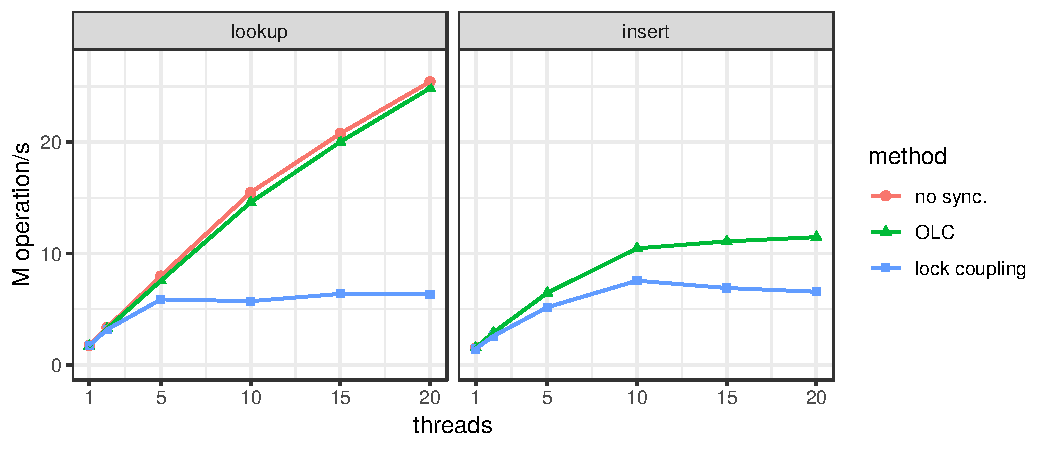
\includegraphics[width=\linewidth]{scale.pdf}
  \vspace{0.2cm}
  \caption{Scalability on 10-core system for B-tree operations (100M values).}
  \label{fig:scale}
\end{figure}

As Figure~\ref{fig:scale} shows, the results change dramatically once we use multiple threads.
For lookup, the scalability of OLC is near-linear up to 20 threads, even though the system has only 10 ``real cores''.
The OLC scalability for insert is also respectable (though not quite as linear because multi-threaded insertion approaches the memory bandwidth of our processor).
The figure also shows that the results of traditional lock coupling with read/write locks are significantly worse than OLC.
With 20 threads, lookup with OLC is 3.9$\times$ faster than traditional lock coupling.

\section{Summary}\label{sec:conc}

Optimistic Lock Coupling (OLC) is an effective synchronization method that combines the simplicity of traditional lock coupling with the superior scalability of lock-free approaches.
OLC is widely applicable and has already been successfully used to synchronize several data structures, including B-trees, binary search trees, and different trie variants.
These features make it highly attractive for modern database systems as well as performance-critical systems software in general.

\begin{thebibliography}{10}

\bibitem{DBLP:conf/spaa/BalmauGHZ16}
O.~Balmau, R.~Guerraoui, M.~Herlihy, and I.~Zablotchi.
\newblock Fast and robust memory reclamation for concurrent data structures.
\newblock In {\em SPAA}, 2016.

\bibitem{DBLP:journals/acta/BayerS77}
R.~Bayer and M.~Schkolnick.
\newblock Concurrency of operations on {B}-trees.
\newblock {\em Acta Informatica}, 9, 1977.

\bibitem{hot}
R.~Binna, E.~Zangerle, M.~Pichl, G.~Specht, and V.~Leis.
\newblock {HOT}: A height optimized trie index for main-memory database
  systems.
\newblock In {\em SIGMOD}, 2018.

\bibitem{DBLP:conf/ppopp/BronsonCCO10}
N.~G. Bronson, J.~Casper, H.~Chafi, and K.~Olukotun.
\newblock A practical concurrent binary search tree.
\newblock In {\em PPOPP}, 2010.

\bibitem{DBLP:conf/vldb/ChaHKK01}
S.~K. Cha, S.~Hwang, K.~Kim, and K.~Kwon.
\newblock Cache-conscious concurrency control of main-memory indexes on
  shared-memory multiprocessor systems.
\newblock In {\em VLDB}, 2001.

\bibitem{intel}
I.~Cutress.
\newblock {Intel} goes for 48-cores: {Cascade-AP} with multi-chip package
  coming soon.
\newblock
  \url{https://www.anandtech.com/show/13535/intel-goes-for-48cores-cascade-ap},
  2018 (accessed January, 2019).

\bibitem{DBLP:conf/cidr/FaleiroA17}
J.~M. Faleiro and D.~J. Abadi.
\newblock Latch-free synchronization in database systems: Silver bullet or
  fool's gold?
\newblock In {\em CIDR}, 2017.

\bibitem{DBLP:journals/ftdb/Graefe11}
G.~Graefe.
\newblock Modern {B}-tree techniques.
\newblock {\em Foundations and Trends in Databases}, 3(4), 2011.

\bibitem{DBLP:conf/hpca/KarnagelDRLLSL14}
T.~Karnagel, R.~Dementiev, R.~Rajwar, K.~Lai, T.~Legler, B.~Schlegel, and
  W.~Lehner.
\newblock Improving in-memory database index performance with
  {Intel}\({}^{\mbox{{\textregistered}}}\) transactional synchronization
  extensions.
\newblock In {\em HPCA}, 2014.

\bibitem{DBLP:journals/tods/LehmanY81}
P.~L. Lehman and S.~B. Yao.
\newblock Efficient locking for concurrent operations on {B}-trees.
\newblock {\em {ACM} Trans. Database Syst.}, 6(4), 1981.

\bibitem{leanstore}
V.~Leis, M.~Haubenschild, A.~Kemper, and T.~Neumann.
\newblock Leanstore: In-memory data management beyond main memory.
\newblock In {\em ICDE}, 2018.

\bibitem{art}
V.~Leis, A.~Kemper, and T.~Neumann.
\newblock The adaptive radix tree: {ARTful} indexing for main-memory databases.
\newblock In {\em ICDE}, 2013.

\bibitem{htmtkde}
V.~Leis, A.~Kemper, and T.~Neumann.
\newblock Scaling {HTM}-supported database transactions to many cores.
\newblock {\em {IEEE} Trans. Knowl. Data Eng.}, 28(2), 2016.

\bibitem{artsync}
V.~Leis, F.~Scheibner, A.~Kemper, and T.~Neumann.
\newblock The {ART} of practical synchronization.
\newblock In {\em DaMoN}, 2016.

\bibitem{DBLP:conf/icde/LevandoskiLS13a}
J.~J. Levandoski, D.~B. Lomet, and S.~Sengupta.
\newblock The {Bw}-tree: A {B}-tree for new hardware platforms.
\newblock In {\em ICDE}, 2013.

\bibitem{DBLP:journals/pvldb/MakreshanskiLS15}
D.~Makreshanski, J.~J. Levandoski, and R.~Stutsman.
\newblock To lock, swap, or elide: On the interplay of hardware transactional
  memory and lock-free indexing.
\newblock {\em {PVLDB}}, 8(11), 2015.

\bibitem{DBLP:dblp_conf/eurosys/MaoKM12}
Y.~Mao, E.~Kohler, and R.~T. Morris.
\newblock Cache craftiness for fast multicore key-value storage.
\newblock In {\em EuroSys}, 2012.

\bibitem{DBLP:journals/tpds/Michael04}
M.~M. Michael.
\newblock Hazard pointers: Safe memory reclamation for lock-free objects.
\newblock {\em {IEEE} Trans. Parallel Distrib. Syst.}, 15(6), 2004.

\bibitem{DBLP:journals/jacm/ShalevS06}
O.~Shalev and N.~Shavit.
\newblock Split-ordered lists: Lock-free extensible hash tables.
\newblock {\em J. {ACM}}, 53(3), 2006.

\bibitem{amd}
A.~Shilov.
\newblock {AMD} previews {EPYC} ‘{Rome}’ processor: Up to 64 {Zen} 2 cores.
\newblock
  \url{https://www.anandtech.com/show/13561/amd-previews-epyc-rome-processor-up-to-64-zen-2-cores},
  2018 (accessed January, 2019).

\bibitem{DBLP:conf/sosp/TuZKLM13}
S.~Tu, W.~Zheng, E.~Kohler, B.~Liskov, and S.~Madden.
\newblock Speedy transactions in multicore in-memory databases.
\newblock In {\em SOSP}, 2013.

\bibitem{buzzword}
Z.~Wang, A.~Pavlo, H.~Lim, V.~Leis, H.~Zhang, M.~Kaminsky, and D.~Andersen.
\newblock Building a {Bw}-tree takes more than just buzz words.
\newblock In {\em SIGMOD}, 2018.

\end{thebibliography}


%\bibliographystyle{abbrv}
%\bibliography{main}

\end{document}

\end{article}
\begin{article}
{Limitations of low dimensional graph embeddings}
{C. Seshadri}
\documentclass[11pt]{article}
\usepackage{amsmath}
\usepackage{amsfonts}
\usepackage{amssymb}
\usepackage{xspace}

\usepackage{caption}
\usepackage{subcaption}

\usepackage{hyperref}


% \newcommand{\eg}{\textit{eg.}}
% \newcommand{\ie}{\textit{i.e.}}

\newcommand{\ks}[1]{\textcolor{red}{[KS: #1]}}

\newcommand{\D}{\text{d}\xspace}

\newcommand{\xbf}{\mathbf{x}\xspace}
\newcommand{\abf}{\mathbf{a}\xspace}
\newcommand{\cbf}{\mathbf{c}\xspace}
\newcommand{\fbf}{\mathbf{f}\xspace}
\newcommand{\ebf}{\mathbf{e}\xspace}
\newcommand{\wbf}{\mathbf{w}\xspace}
\newcommand{\vbf}{\mathbf{v}\xspace}
\newcommand{\ubf}{\mathbf{u}\xspace}
\newcommand{\sbf}{\mathbf{s}\xspace}
\newcommand{\Sbf}{\mathbf{S}\xspace}
\newcommand{\Xbf}{\mathbf{X}\xspace}
\newcommand{\Zbf}{\mathbf{Z}\xspace}
\newcommand{\zbf}{\mathbf{z}\xspace}
\newcommand{\ybf}{\mathbf{y}\xspace}
\newcommand{\dbf}{\mathbf{d}\xspace}
\newcommand{\bbf}{\mathbf{b}\xspace}
\newcommand{\mbf}{\mathbf{m}\xspace}

\newcommand{\onebf}{\mathbf{1}\xspace}
\newcommand{\zerobf}{\mathbf{0}\xspace}
\newcommand{\threebf}{\mathbf{3}\xspace}

\newcommand{\Gbf}{\mathbf{G}\xspace}
\newcommand{\Abf}{\mathbf{A}\xspace}
\newcommand{\Bbf}{\mathbf{B}\xspace}
\newcommand{\Ubf}{\mathbf{U}\xspace}
\newcommand{\Vbf}{\mathbf{V}\xspace}
\newcommand{\Dbf}{\mathbf{D}\xspace}
\newcommand{\Ebf}{\mathbf{E}\xspace}
\newcommand{\Qbf}{\mathbf{Q}\xspace}
\newcommand{\Lbf}{\mathbf{L}\xspace}
\newcommand{\Ibf}{\mathbf{I}\xspace}
\newcommand{\Mbf}{\mathbf{M}\xspace}

\newcommand{\Lambdabf}{\bm{\Lambda}\xspace}
\newcommand{\lambdabf}{\bm{\lambda}\xspace}
\newcommand{\mubf}{\bm{\mu}\xspace}
\newcommand{\epsbf}{\bm{\epsilon}\xspace}
\newcommand{\Sigmabf}{\bm{\Sigma}\xspace}
\newcommand{\Thetabf}{\bm{\Theta}\xspace}
\newcommand{\one}{\mathds{1}\xspace}
\newcommand{\trace}{\text{tr}\xspace}


\newcommand{\CG}{G\xspace}
\newcommand{\CV}{V\xspace}
\newcommand{\CT}{\mathcal{T}\xspace}
\newcommand{\CE}{E\xspace}
\newcommand{\CA}{\mathcal{A}\xspace}
\newcommand{\CB}{\mathcal{B}\xspace}
\newcommand{\CD}{\mathcal{D}\xspace}
\newcommand{\CX}{\mathcal{X}\xspace}
\newcommand{\CY}{\mathcal{Y}\xspace}
\newcommand{\CK}{\mathcal{K}\xspace}
\newcommand{\CM}{\mathcal{M}\xspace}
\newcommand{\CC}{\mathcal{C}\xspace}
\newcommand{\CL}{\mathcal{L}\xspace}
\newcommand{\CI}{\mathcal{I}\xspace}

\newcommand{\Mod}[1]{\ (\mathrm{mod}\ #1)}

\newtheorem{prob}{Problem}

\begin{document}

\title{Limitations of low dimensional graph embeddings}

\author{C. Seshadhri\footnote{University of California, Santa Cruz. {\tt sesh@ucsc.edu}. Supported by NSF DMS-2023495, CCF-1740850, 1839317, 1908384}}

\date{}
\maketitle
\renewcommand\thesection{\arabic{section}}
\setcounter{section}{0}
\setcounter{figure}{0}
\setcounter{table}{0}

\begin{abstract}
The learning of graph representations, also called graph embeddings, is a fundamental technique in machine learning (ML).
The aim is to represent the vertices of a graph by low-dimensional real-valued vectors, which can be 
used for a variety of downstream ML tasks. The popular technique of Graph Neural Networks (GNNs) can
be thought of a type of graph representation learning method. This article surveys some recent work on the \emph{limitations}
of graph embedding methods. These results provide mathematical theorems proving that low-dimensional
embeddings cannot recreate ``community-like" structure, through commonly used kernels. These theorems
are supported by empirical results, showing that many classic graph embedding methods actually perform
poorly on important machine learning tasks. Low-dimensional representations often lose
much of the fine-grained community structure of real-world data. The results surveyed in this article
provide an interesting counterpoint to the popularity of graph embeddings and GNNs for machine learning.
\end{abstract}

\section{Introduction}

Capturing the rich structure of graph is central for many machine learning tasks.
The heterogenous, non-local, and massive structure
of modern graphs are a problem for many basic machine learning tasks,
such as ranking, link prediction, and classification~\cite{easley2010networks}.
\emph{Graph representation learning} provides a
convenient solution to this problem. Each vertex
of a graph is represented as a vector in low-dimensional space. 
These vectors form the (low-dimensional) embedding of the graph.
The vectors can be used for a plethora of downstream machine learning tasks.
The aim is to have these vectors combine the graph structure with vertex features into
a compact geometric representation.

The study of low-dimensional graph embeddings is an incredibly popular
research area, and has generated many exciting results over the past
few years (see surveys~\cite{HaYiLe18, MLGSurvey20} and a Chapter 23 in~\cite{pml1Book}). 
The most successful methods for graph embeddings often use Deep Learning techniques,
together with classic approaches like matrix factorization~\cite{PeAlSk14,GrLe16,OuCu16,PeKu+17,QiDo18,LiWu19}. Graph Neural Networks (GNNs)
can be thought of as specific class of graph embeddings algorithms~\cite{HaYiLe17,VeCu+18,XuHuLe+19}.
Despite the large variety of algorithms used for graph representation learning (and specifically GNNs),
their output has a simple, consistent structure. Given a graph $G$ on $n$
vertices, these methods map each vertex to a vector in $\sRR^d$, where
$d \ll n$. In a typical applications, $n$ is the order of millions or more,
while $d$ is in the hundreds.

Much of the advances in this field are primarily empirical; there
are numerous papers in major machine learning conferences on more
complex GNN architectures or more involved graph embedding methods.
Nonetheless, there is limited principled understanding of the power of low-dimensional
graph embeddings. Small changes in training or input data can lead to major differences
in the output~\cite{GuVi+19}. Much of the research on graph embeddings and GNNs, for example, report significant success in prediction
tasks on graphs~\cite{GrLe16,HaYiLe17,QiDo18}. On the other hand, some papers suggest that low-dimensional graph embeddings
can be beaten by simpler hand-tuned methods~\cite{GuVi+19,HuHe+21}.
It is useful to have a rigorous mathematical framework to understand graph embeddings.
Specially, we wish to address the following questions.

\begin{asparaitem}
    \item To what extent can relevant graph structure be captured by low-dimensional graph embeddings?
    \item How does low-dimensional geometry relate to downstream ML tasks on graphs?
    \item How does the choice of kernel functions (for prediction tasks) affect the task?
\end{asparaitem}

\medskip

Contrary to most research in this area, our approach to investigating these questions is through \emph{limitations}
or lower bounds. Our aim is develop a theoretical framework that is agnostic to the specific
algorithm performing the embedding. We first describe some basic terminology and central concepts.

\paragraph{The importance of matrix factorizations:} A low-dimensional matrix factorization approximates
gives an algorithm-independent view of how low-dimensional embeddings represent graphs. We think
of $M$ as an adjacency matrix, or any matrix representation of our graph $G$. In many Deep Learning
methods, $M$ is constructed by long walks with appropriate vertex-centric aggregation functions~\cite{PeAlSk14,GrLe16,PeKu+17}.
The matrix $V$ is the collection of embeddings, where each column vector corresponds to a vertex.
Recent work has shown the many different graph embedding methods can be cast as matrix factorizations,
with different choices of matrices $M$, and different notions of approximations~\cite{QiDo18}. Indeed, the simplest
low-dimensional embedding is obtained by a low-rank SVD of the adjacency matrix, arguably the most
basic of matrix factorizations.

\medskip

\paragraph{The importance of dot products:} Regardless of how the graph embedding vectors are obtained,
the general strategy is to use ``nearness" in geometric space as a proxy for the similarity of the corresponding
vectors. Thus, the downstream ML tasks treat vertices $i$ and $j$ as similar if their corresponding
vectors $\vec{v}_i$ and $\vec{v}_j$ are similar. Arguably, the most important measure of similarity is 
the dot product $\vec{v}_i \cdot \vec{v}_j$ or cosine similarity (which is a normalized dot product). 
This has special significance for matrix factorizations,
since $V^TV$ is precisely the matrix of all pairs of dot products.

Even when the embedding vectors are not obtained by matrix factorizations, the Gram
matrix $V^TV$ is commonly used for downstream prediction tasks. A natural strategy for any prediction task 
is to use nearest neighbor (k-NN) search according to the dot product/cosine similarity. There are many open course packages for k-NN, making it 
the default choice in industrial applications of graph embeddings~\cite{Sci}. 

\medskip

We now can formalize our initial questions in matrix language. 
Observe how there is no reference to any embedding method or GNN;
we directly analyze the behavior of the output representation.

\begin{center}
Can a Gram matrix $V^TV$ for $V \in \sRR^{d \times n}$ ($d \ll n$)
capture the structure of either real-world networks
or the properties of prediction matrices arising from downstream ML tasks
(on graphs)?
\end{center}

This framework captures the vast majority of graph embedding constructions and applications.

\subsection{Limitations of graph embeddings} \label{sec:limit}

This article presents two results on the limitations of low-dimensional graph embeddings
for prediction and machine learning on real-world graphs~\cite{SeSh20,StLe+22}. The underlying
theoretical results are algorithm agnostic, and the limitations hold for \emph{any} graph embedding
algorithm. These results come with empirical backing, performed on classic and important graph
embedding methods.

\paragraph{Inability to recreate triangle structure~\cite{SeSh20}:} This result focuses
on the fundamental premise of low-dimensional embeddings, rather than a specific ML task. 
Algorithms to construct (or predict from) low-dimensional embeddings implicitly pose
a low-dimensional graph/matrix model. This model represents a distribution of graphs
that are created from a set of real vectors (where each vector represents a vertex). The embedding
is constructed by fitting this model to an input graph, typically using dot product as a 
proximity measure.

This result mathematically proves that no low-dimensional model (using a dot product kernel) can simultaneously
recreate two central properties of real-world graphs: sparsity and triangle density. It is well-known
from the early days of network science that real-world graphs are sparse but have high clustering
coefficients~\cite{WaSt98,SaCaWi+10,SeKoPi12,DuPi+12}. Hence, typical models used to construct low-dimensional embeddings cannot
generate realistic graphs. They miss the (crucial) triangle structure of real data.

The theory is supported with empirical results. These empirical results are demonstrated
on other kernels beyond the dot product, thus suggesting that the limitations are fundamental.
We discuss these results in \Sec{imp-tri}.

There are notable counterpoints to these results.
Firstly, Chanpuriya et al show that asymmetric embeddings avoid the rank lower bounds
discussed above~\cite{CMST20}. Another result of Chanpuriya et al shows that graphs can sometimes be
reconstructed from their embeddings. In some cases, the community structure of the reconstruction
is actually enhanced~\cite{ChMu+21}. We give more detail in \Sec{imp-tri}.

\paragraph{Weak performance on community labeling tasks~\cite{StLe+22}:} This result takes
a complementary angle, and focuses on a downstream ML task. Community labeling is a binary
prediction problem, where we wish to predict if two vertices belong to a community.
This work sets up a community labeling problem for both real and synthetic data sets. First,
the authors create a simple benchmark algorithm using logistic regression on classic graph 
features (like Personalized PageRank and short path counts). This benchmark has fairly
good performance, as measured by distributions of local precision. On the other hand,
many well-established graph embedding methods have surprisingly poor performance
on the same task.

These observations are backed up with theoretical proofs. The prediction matrices
based on low-dimensional embeddings provably do not have the typical community
structure of real data. This work also investigates alternate kernels,
like the normalized softmax (used in results like {\tt DeepWalk} and {\tt node2vec}~\cite{PeAlSk14,GrLe16}).
These kernels have other limitations in that slight noise can destroy community
structure in the corresponding prediction matrices.

These results are discussed in \Sec{poor-comm}.

\subsection{Broader context} \label{sec:context}

A reader may ask: how are the limitations stated in this article consistent
with large body of work on the effectiveness of graph embeddings and GNNs?
Our answer is two-fold, backed up by~\cite{GuVi+19,HuHe+21}. First, most research on graph embeddings compare various representation
learning methods with each other, and do not consider alternative baselines. Secondly, we believe that many graph embeddings methods do not 
have good predictions with respect to other metrics. For example, almost all
these result use the AUC metric to measure link prediction performance. On the other hand,
AUC is a bad measure for sparse ground truth~\cite{Ha09,LiCh12}. Indeed, in \Sec{poor-comm},
we show poor prediction performance (for graph embedding methods) on a local precision metric.

There has been compelling empirical work showing that GNNs and embeddings can be 
outperformed by simpler methods. We mention two results in detail because
they highlight empirical weaknesses in graph embeddings, and reinforce the
previous points.

{\bf Gurukar et al, the lack of good experimental design~\cite{GuVi+19}:} Gurukar et al do a detailed comparison of twelve
different graph representation learning methods on a variety of ML tasks. They focus on two
of the most important tasks of link prediction and node classification. Despite
there being many newer methods, they observe that the {\tt M-NMF} algorithm
is best for link prediction~\cite{WaCu+17} and {\tt NetMF} algorithm~\cite{QiDo18} is best for node classification.
No graph representation method outperforms on both metrics. This paper does an exceptional
job of clearly specifying the experimental design and thoroughly investigating previous work.

Along the lines of the current article, simple task specific baselines are competitive with
graph embedding methods. These baselines are formed by a simple model that uses basic graph features
(like Common Neighbors, Adamic-Adar index~\cite{AdAd03}, Jaccard similarity, etc.). These results
are analogous to what we observe in~\cite{StLe+22}. 

Gurukar et al point out a major problem with evaluations in graph embedding papers.
Quoting from there: ``$\ldots$ a new method
almost always compares its performance against a subset of
other methods [and] datasets previously evaluated. While great care is taken
to tune the new method, the same care is often not taken when evaluating baselines."

{\bf Huang et al, easier methods beat GNNs~\cite{HuHe+21}:} Huang et al devise
an alternate graph learning algorithm called \emph{Correct and Smooth (C\&S)}.
Consider the problem of node classification. This method starts with a ``base predictor"
that ignores the graph structure. Using only node features, one can train
a basic model for classification. Then, the graph is introduced a post-processing
step to ``correct and smooth" the errors. The idea is that the errors should be correlated along edges.
So this method tries to find a smooth error estimation on the graph, which 
is computed using standard label propagation methods. This smoothed error estimate is
used to correct the base predictor.

The C\&S method is shown to outperform GNNs on node classification tasks on
the OGB leaderboard~\cite{ogb}. In some cases, a state-of-the-art GNN has slightly
better performance, but the GNNs always have many orders of magnitude more parameters.
Hence, it is much more expensive to train them than C\&S.

\medskip

We also mention another line of weaknesses, specific to message passing GNN architectures.
These results show that certain graph-theoretic properties cannot be learned by common
GNN architectures~\cite{XuHuLe+19,Lo20,GaJeJa20}. There are formal limits on what
GNN-based representations can learn. Some of these results show that message passing GNNs 
are no more powerful than the classic Weisfeiler-Lehman (WL) isomorphism test~\cite{XuHuLe+19}.

The work presented in the current article
is different from these results because of the (algorithm agnostic) focus on the geometry of graph representations.

\section{Impossibility of capturing sparse, triangle-rich structure} \label{sec:imp-tri}

The first result we present argues that low-dimensional embeddings with
dot product geometries are \emph{not} good representation of real-world graphs.
Seshadhri, Sharma, Stolman, and Goel demonstrate mathematically and empirically that they lose local cluster structure,
a central aspect of graphs that arise from real data~\cite{SeSh20}.

Graph embeddings are often generated by assuming that the embeddings vectors lie
in a hidden, latent space. We assume a model that generates graphs from these vectors,
which can be thought of as the model parameters. The embeddings are constructed
by optimizing for these parameters, given the input graph.

Consider the graph embedding vectors $\vec{v}_1, \vec{v}_2, \ldots, \vec{v}_n \in \mathbb{R}^d$
(denoted by the $d \times n$ matrix $V$).
Let $\cG_V$ denote the following distribution of graphs over the vertex set $[n]$.
For each index pair $i,j$, independently insert (undirected) edge $(i,j)$ with probability
$\max(0,\min(\vec{v}_i \cdot \vec{v}_j, 1))$. (If $\vec{v}_i \cdot \vec{v}_j$ is negative,
$(i,j)$ is never inserted. If $\vec{v}_i \cdot \vec{v}_j \geq 1$, $(i,j)$ is always inserted.)
This model subsumes the classic Stochastic Block Model~\cite{HoLa83}
and Random Dot Product Model~\cite{YoSc07,AtFi+18}. Many graph embedding methods,
including GNNs, effectively optimize over such a model to generate
the embedding vectors.

% 
% 
% There are 
% alternate models that use different functions of the dot product
% for the edge probability, which are discussed in Section~\ref{sec:variants}
% Matrix factorization is a popular method to obtain such a vector representation: the original adjacency matrix $A$
% is ``factorized" as $V^TV$, where the columns of $V$ are $\vec{v}_1, \vec{v}_2, \ldots, \vec{v}_n$.

\begin{figure}
        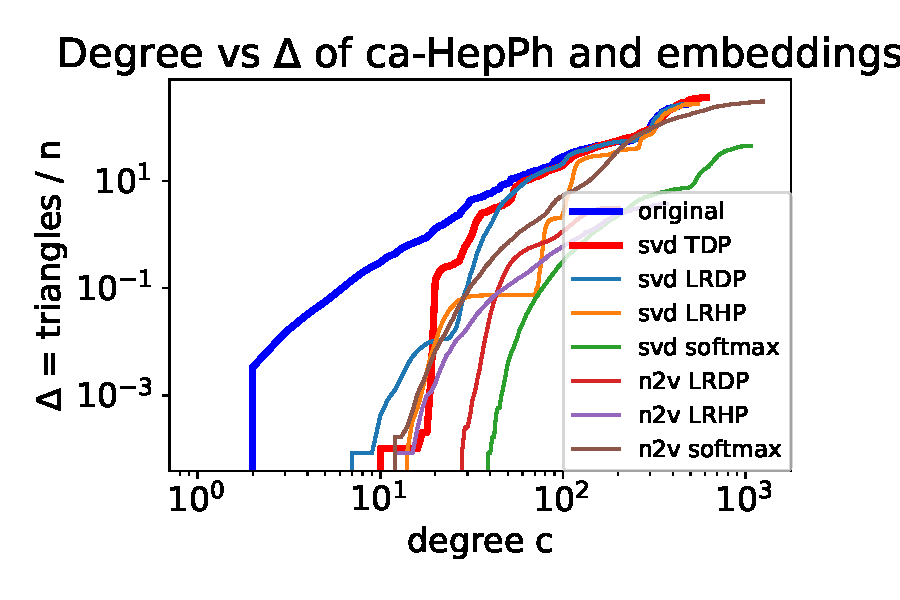
\includegraphics[scale=.35]{submissions/Seshadri2023/figures/ca-HepPh_tri_distro.pdf}
        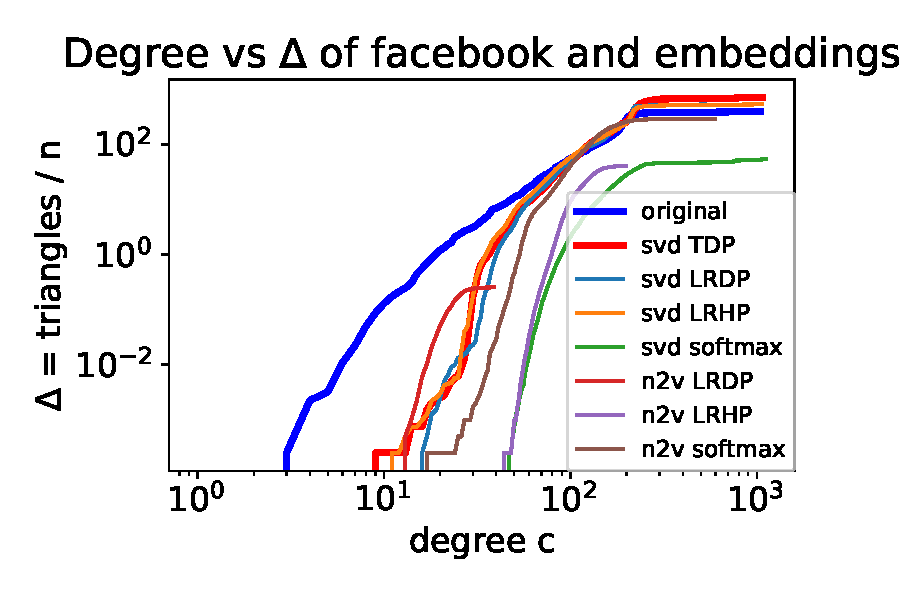
\includegraphics[scale=.35]{submissions/Seshadri2023/figures/facebook_tri_distro.pdf}
        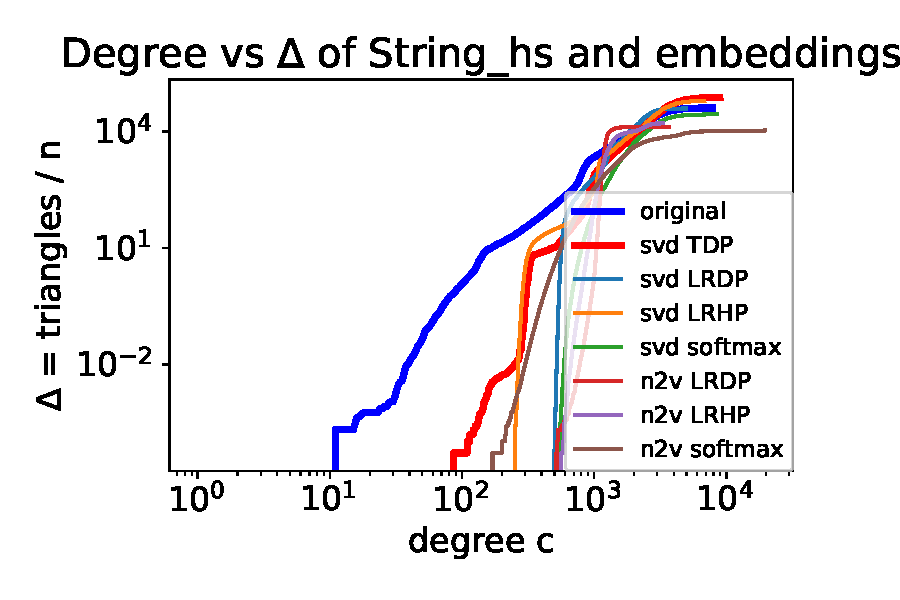
\includegraphics[scale=.35]{submissions/Seshadri2023/figures/String_hs_tri_distro.pdf} 
%         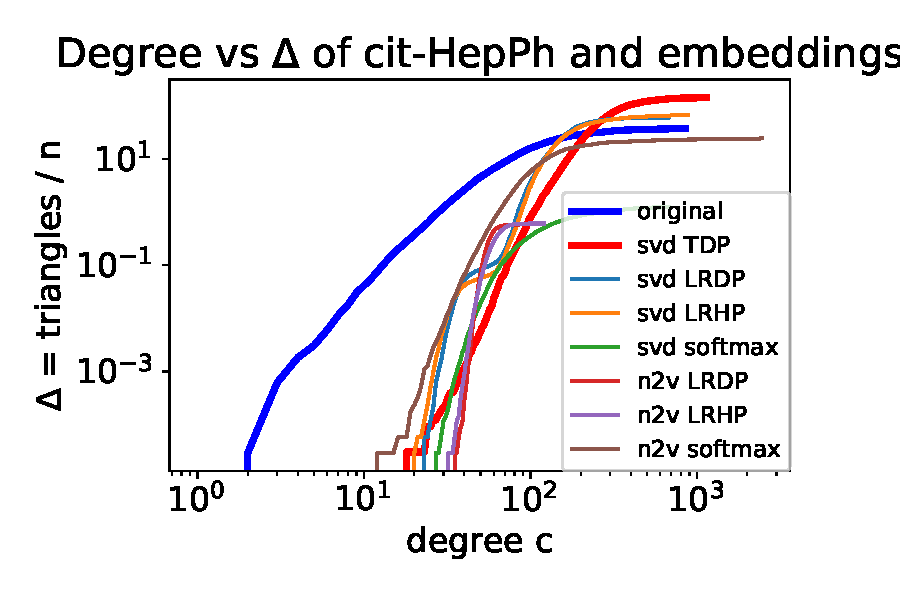
\includegraphics[scale=.37]{submissions/Seshadri2023/figures/cit-HepPh_tri_distro.pdf}
				\captionof{figure}{\small Plots of degree $c$ vs $\Delta$: We plot results for a variety
                of real-world graphs: (i) {\tt ca-HepPh}, a High Energy Physics coauthorship network (ii)
                {\tt Facebook}, a small snapshot of a Facebook social network, (iii) {\tt String\_hs}, a Protein-protein interaction network.
        We plot $c$ versus the total number of triangles only involving vertices of
        degree at most $c$. We divide the latter by the total number of vertices $n$,
        so it corresponds to $\Delta$, as in \Def{foundation}. We plot these
        both for the original graph (in thick blue), and for a variety of embeddings and kernel functions.
        For each embedding, we plot the maximum $\Delta$ in 
        a set of 100 samples from a 100-dimensional embedding. The embedding analyzed by
        \Thm{main} (TDP) is given in thick red. Observe how the embeddings generate
        graphs with very few triangles among low degree vertices. The gap in $\Delta$ for low degree is
        2-3 orders of magnitude. The other lines correspond to alternate embeddings,
        using the {\sc node2vec} vectors and/or different functions of the dot product.} \label{fig:intro-triangle-distro}
\end{figure}

Two hallmarks of real-world graphs are: (i) Sparsity: average degree is constant with respect
to $n$, and (ii) Triangle density: there are many triangles incident to low degree vertices~\cite{WaSt98,SaCaWi+10,SeKoPi12,DuPi+12}.
The large number of triangles is an important aspect of community structure. 

\begin{definition} \label{def:foundation} For parameters $c > 1$ and $\Delta > 0$, a graph $G$ with $n$ vertices
has a \emph{$(c,\Delta)$-triangle foundation} if there are at least $\Delta n$ triangles contained among vertices of degree at most $c$.
% Formally, let $S_c$ be the set of vertices of degree at most $c$. Then, the number of triangles
% in the graph induced by $S_c$ is at least $\Delta n$.
\end{definition}

Typically, we think of both $c$ and $\Delta$ as constants. 
{We emphasize that $n$ is the total number of vertices in $G$, not the number
of vertices in $S$.}
In Figure~\ref{fig:intro-triangle-distro}, we plot the value
of $c$ vs $\Delta$ as the thick blue line. (Specifically, the $y$ axis is the number of triangles divided by $n$.)
Observe that for all graphs,
for $c \in [10,50]$, we get a value of $\Delta > 1$ (in many cases $\Delta > 10$). 
As mentioned earlier, there is much work in network science showing that there are often a linear
number of triangles among low degree vertices~\cite{SeKoPi12,DuPi+12}.

Our main result is that \emph{any} embedding of graphs that generates graphs with $(c,\Delta)$-triangle foundations,
with constant $c,\Delta$, must have near linear rank. This
contradicts the belief that low-dimensional embeddings capture the structure of real-world complex networks.

\begin{theorem} \label{thm:main} Fix constant $c > 4, \Delta > 0$. Suppose the expected number of triangles 
in $G \sim \cG_V$ that only involve vertices of expected degree $c$ is at least $\Delta n$.
Then, the rank of $V$ is at least $\Omega(n/\lg^2n)$.
\end{theorem}

Equivalently, graphs generated from low-dimensional embeddings cannot contain many
triangles only on low-degree vertices. In all applications, $d$ is thought of as a constant,
or at least much smaller than $n$. On the contrary, \Thm{main} implies
that $d$ must be $\Omega(n/\lg^2n)$ to accurately model the low-degree triangle behavior.
This lower bound holds \emph{regardless} of how the vectors are constructed. 


\subsection{Empirical validation} \label{sec:emp}

% While the polynomials
% involved in Theorem~\ref{thm:main} are large,
We empirically validate the theory on a collection of complex
networks. For each real-world graph, we compute a 100-dimensional embedding through 
SVD and an important Deep Learning method, {\tt node2vec}~\cite{GrLe16}.
We generate $100$ samples of graphs from these embeddings, and compute
their $c$ vs $\Delta$ plot. This is plotted with the true $c$ vs $\Delta$ plot.
(To account for statistical variation, we plot
the \emph{maximum} value of $\Delta$ observed in the samples, over all graphs. The variation
observed was negligible.)
\Fig{intro-triangle-distro} shows such a plot for three different real-world networks.
 
In all cases, this plot is significantly off the mark at low degrees for the embedding. Around the lowest degree,
the value of $\Delta$ (for the graphs generated by the embedding) 
is 2-3 orders of magnitude smaller than the original value.
The local triangle structure is destroyed around low degree vertices.
The total number of triangles is preserved well, as shown
towards the right side of each plot. A nuanced view of the triangle
distribution, as given in \Def{foundation}, is required to see the shortcomings
of low dimensional embeddings.

We note that several other functions of dot product have been
  proposed in the literature, such as the softmax
  function~\cite{PeAlSk14,GrLe16} and linear 
models of the dot product~\cite{HaYiLe17}. \Thm{main} does not have
direct implications for such models, but our empirical validation holds for 
them as well. The embedding in Theorem~\ref{thm:main} uses the \emph{truncated
dot product} (TDP) function $max(0,\min(\vec{v}_i \cdot \vec{v}_j, 1))$ to model
edge probabilities. We construct other embeddings that compute edge probabilities
using machine learning models with the dot product and Hadamard product
as features. This subsumes linear models as given in~\cite{HaYiLe17}. 
We also consider (scaled) softmax functions, as in~\cite{PeAlSk14}, and standard
machine learning models (LRDP, LRHP). 

For each of these models, we perform the same experiment described above.
\Fig{intro-triangle-distro} also shows the plots for these other models.
Observe that \emph{none} of them capture the low-degree triangle structure,
and their $\Delta$ values are all 2-3 orders of magnitude lower than the original.  
Chanpuriya et al also validate these results on various other embedding methods~\cite{CMST20}.

\subsection{Counterpoints} \label{sec:counter}

We discuss two important results of Chanpuriya, Musco, Sotiropoulos, and Tsourakakis~\cite{CMST20,ChMu+21}.
The first result show that the rank lower bound of \Thm{main} can be circumvented
with an asymmetric embedding. They prove that one can construct \emph{two} matrices
$U, V \in \sRR^{d \times n}$ such that the graph distribution from $UV^T$ can generate
realistic triangle structure. They show that any bounded degree graph can be embedded
in this method with at most max-degree dimensions. This introduces a new technique
for graph embeddings. We note, however, that such asymmetric embeddings lose the geometric
structure of the standard embeddings. One wants geometric proximity of vectors to
represent structural closeness. For vertices $i$ and $j$, an asymmetric embedding approximates the edge probability
by $\vec{u}_i \cdot \vec{v}_j$, but the similarity of $i$ and $j$ would be measured
by looking at (say) $\vec{u}_i$ and $\vec{u}_j$. It would be interesting to incorporate similarity
in asymmetric embeddings.

Another result shows that, in some cases, community structure can be reconstructed
from {\tt DeepWalk} embeddings~\cite{ChMu+21}. This shows that some structure
is being retained by the embeddings. We note that these results mostly
focus on SBMs with a constant (at most 5) blocks, or only the largest few communities
in real data. \Thm{main} and the other results in this article focus on cases where
the number of blocks/communities is large. We believe that low-dimensional embeddings
can recover the top few communities, but fail to capture the rich structure 
of many small communities. In the next section, we discuss this point further.



\section{Challenges for community labeling using graph embeddings} \label{sec:poor-comm}

One central promise of unsupervised graph embedding methods is to
preserve network structure in the geometry.
To what extent do embedding methods capture
graph structure relevant to downstream ML tasks?

This section is based on the paper of Stolman, Levy, Seshadhri, and Sharma~\cite{StLe+22}.
We begin this discussion with the empirical results, because they
highlight the core observation. After that, we will go into the mathematical
explanations that relate to low-dimensional embeddings and factorization.

Consider the following well-defined \emph{pairwise
  community labeling} problem. Given two vertices $i$ and $j$, the
binary classification task is to determine whether they belong to the
same community. We note that this community labeling problem is an
instance of a broad range of community detection problems that have a
long history of study in the graph mining
literature~\cite{mmds_book}. 


\subsection{Empirical setup} \label{sec:comm-setup}

We use a set of real-world datasets with ground truth community labels,
an Amazon co-purchase graph of products and a DBLP citation network~\cite{YaLe12}.
We also create a synthetic Stochastic Block model, with 100K vertices,
and small blocks of size $20$ each. There is a dense graph within each block,
and a random sparse graph connecting all the blocks.

As explained earlier, the prediction task is to determine if an input pair $i, j$
of vertices belong to a community. (They may belong to multiple communities;
to make the problem simpler, we do not require any community labels to be determined.)

\begin{figure*}[h]
\begin{tabular}{c c c}
	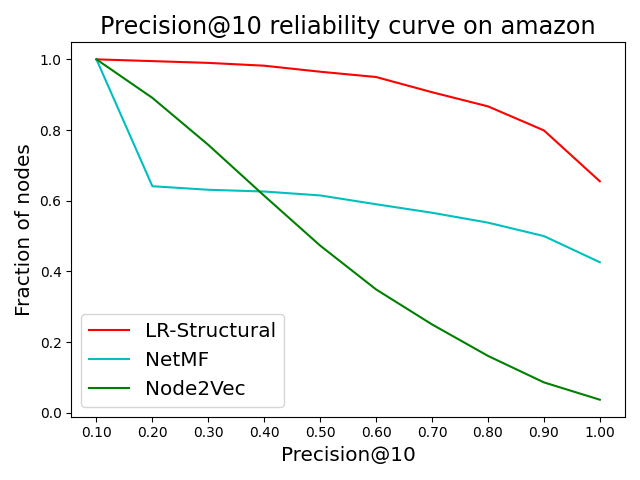
\includegraphics[width=.33\linewidth]{submissions/Seshadri2023/figures/amazon_curves.png} &
	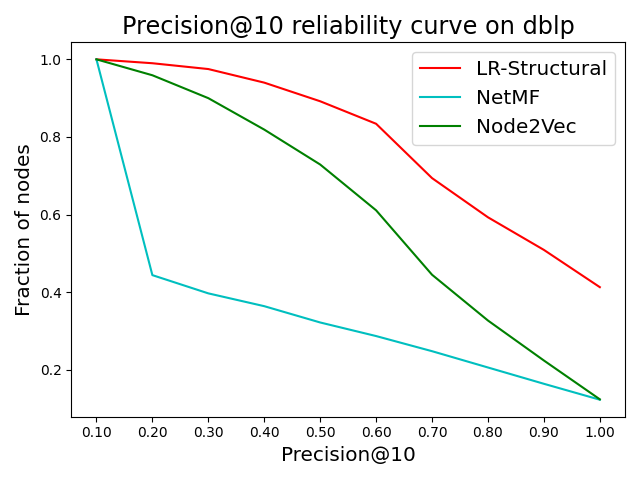
\includegraphics[width=.33\linewidth]{submissions/Seshadri2023/figures/dblp_curves.png}  &
	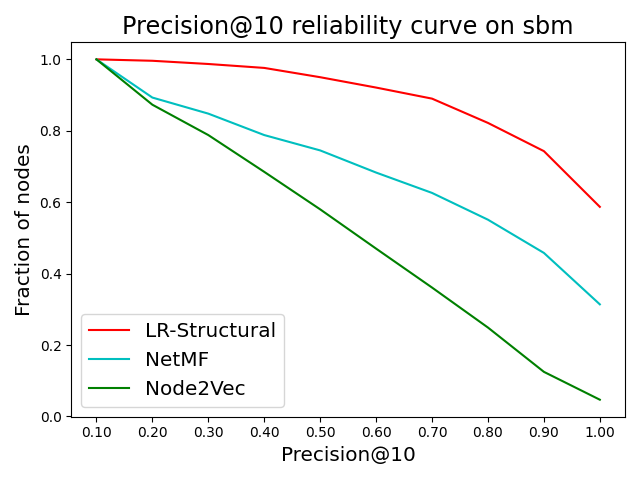
\includegraphics[width=.33\linewidth]{submissions/Seshadri2023/figures/sbm_curves.png}
\end{tabular}
\caption{Each point, $(x, y)$, on the curve represents the approximate fraction of vertices, $y$, for
	which the given method produces a precision@10 score of at least $x$. \slr is plotted against
the two best performing embedding methods. $1000$ vertices are sampled and for each vertex $v$ sampled,
the vertices of the graph
$u_1, \ldots, u_n$, are ordered by decreasing score assigned by the given classifier.
The precision@10 is the fraction of $u_1, \ldots, u_{10}$ which share a community with $v$.
Across all instances, the simple baseline $\slr$ handily outperforms more complex graph embedding methods.
}
\label{fig:p10-curves}
\end{figure*}

\paragraph{The setup for graph embeddings:} We experiment with a set of important graph
embedding methods based on factorizations and Deep Learning ({\tt{GraRep, DeepWalk, node2vec, NetMF}}~\cite{PeAlSk14,CaLu15,OuCu16,GrLe16,QiDo18}).
We note that the {\tt NetMF} method was reported to be one of the best embedding methods for node classification~\cite{GuVi+19}.
Given the embedding for each vertex, we need to construct pairwise features for pairs in $(i,j) \in V \times V$,
for the community prediction task.
The standard approach is to either take the dot product $\vec{v}_i \cdot \vec{v}_j$
or the Hadamard product $\vec{v}_i \circ \vec{v}_j$. (Recall 
that the Hadamard product is a $d$-dimensional vector whose $r$th coordinate
is the product of the $r$th coordinates of $\vec{v}_i$ and $\vec{v}_j$.)
We finally train a logistic regression model on these features for the prediction problem.
This is the standard pipeline used in prior work~\cite{covington2016deep,GrLe16,MLGSurvey20}. 

\paragraph{A simple baseline:} We compute four basic structural graph features for pairs
of vertices $(i,j)$. We look at the cosine similarity and cut size between neighborhoods, and
the Personalized PageRank values. These are well-known classic features used in the literature~\cite{SSG17,ACL07}.
We train a simple logistic regression model on these four features; the model is denoted \slr.

\paragraph{Performance metric:} For both real and simulated data, the ground truth is
sparse, i.e. the vast majority of node pairs do not belong to the same
community. We do not use AUC because of its problems in measuring
sparse data~\cite{Ha09,LiCh12}. Instead, it is appropriate to measure the prediction
performance using precision-recall curves for this highly imbalanced
label distribution~\cite{DG06}. 

The methods are evaluated by comparing the ``precision@10" distributions.
We sample 1000 random vertices. For each of 1000 vertices sampled, $v$, 
we order the other vertices of the graph, $u_1, \ldots, u_n$, in decreasing
order of their prediction score. (The model predictors based on logistic regression
on the embedding vectors or structural features assign a score in $[0,1]$.) 
We compute the precision, per vertex, of the classifier among the top 10 scores, 
with respect to the ground truth.
When the predictor is based on dot product, this is simply the top 10 neighbors
in geometric space.
In other words, we sample a vertex at random and report
the fraction of its ten nearest neighbors with which it shares a community.

We represent the distribution of values of precision@10 scores as a reliability curve. This is the curve
$(x, y)$ such that at least a $y$ fraction of vertices sampled had a precision@10 score score of at least $x$.
Higher $y$ values for a given $x$ indicate better performance.
\Fig{p10-curves} contains the curves for the best methods against the baseline (we leave out methods
with poorer performance).

\paragraph{Main observation:} Across \emph{all instances}, the baseline \slr method heavily outperforms
the more complex graph embedding methods. The performance gap for the simple Stochastic Block Model
instance is striking. The graph is practically learnable (just a collection of dense blocks with sparse connections),
but the embedding methods fail to accurately predict pairs within blocks.
For the \slr method, in all instances, at least 90\% of the vertices have a precision@10 of at least $0.5$.
This means, for at least 90\% of the vertices, at least five of the top 10 scores are in the same
community. By contrast, for the embedding methods, this fraction is less than 75\%. When looking
for a precision of more than $0.8$, the embeddings methods have less than 20\% of vertices
achieving high scores. Overall, we observe that the embeddings methods do not perform
the community labeling task well, despite the simple \slr baseline having good precision values.

\subsection{Theoretical explanation of limitations} \label{sec:theory-comm}

As explained earlier, a large variety of graph embedding methods (including
those using Deep Learning) implicitly factorize a matrix $M$
as $V^TV$. Here, $M$ denotes some matrix representing the input graph data
or the final prediction, and $V \in \sRR^{d \times n}$ is the matrix of graph embeddings.
Broadly speaking, we can
classify these methods into two categories:

\begin{asparaitem}
    \item {\bf Direct factorizations:} Here, we set $V$ as \\$\argmin_V \|V^TV - M\|_2$, where $M$ is typically
    (some power of) the graph adjacency matrix. Methods such as Graph Factorization, GraRep~\cite{CaLu15},
    and HOPE~\cite{OuCu16} would fall under this category.
    \item {\bf Softmax factorizations:} These methods factorize a stochastic matrix, such as (powers of)
    the random walk matrix. (A stochastic matrix has row sums equal to one.) Since $V^TV$ is not necessarily stochastic, these methods apply the softmax
    to generate a stochastic matrix. Notable examples are such methods are DeepWalk~\cite{PeAlSk14} and Node2vec~\cite{GrLe16}.
    Formally, consider the normalized softmax matrix $\sm(V)$ given by 
% Our aim is to show that
% embedding methods based on the softmax function must have high rank. Formally,
% the embedding method produces vectors $\vec{v}_1, \vec{v}_2, \ldots,
% \vec{v}_n$. Let $V$ denote the matrix where these vectors are columns. Methods
% like Deepwalk and node2vec model $M$ as follows. Consider the Gram matrix
% $V^TV$, and define matrix $\tM$ where
\begin{equation}
\sm(V)_{ij} = \frac{\exp(\vec{v}_i \cdot \vec{v}_j)}{\sum_k \exp(\vec{v}_i \cdot \vec{v}_k)}
\end{equation}
Note that $\sm(V)$ is stochastic by construction. 
\end{asparaitem}

The {\tt NetMF}~\cite{QiDo18} method interpolates between these categories and shows
that a number of existing methods can be expressed as factorization methods, especially
of the above forms.

% The embeddings are based
% on the Gramian (dot product) matrix $V^TV$, and thus, it is natural to
% see the extent to which the dot product predicts the community
% structure. This measures
% the ability of geometric similarity (dot product) to predict community similarity.
% We note that the dot product is commonly used in
% previous work on graph embeddings~\cite{MLGSurvey20}. 

\paragraph{The notion of community pairs:} We start with an abstraction of community structure from a matrix
standpoint: many dense
blocks in an overall sparse matrix. We quantify ``how
much" community structure can be present in a matrix $V^TV$ or
$\sm(V)$, for any matrix $V \in \sRR^{d\times n}$ (for
$d \ll n$). This formulation captures the fundamental notion of
a low-dimensional embedding, without referring to any specific method
to compute it. 

Let us start with an $n \times n$ matrix $M$ that represents the ``similarity" or likelihood of connection
between vertices. This is the final prediction matrix for community labeling. 
For convenience, let us normalize so that the $\forall i \in [n], \sum_{j \leq n} M_{i,j} \leq 1$.
(So the sum of similarities of a vertex is at most $1$.) A communities is essentially
a dense block of entries, which motivates the following definition. 
We use $\seps$ to denote a parameter for the threshold of community strength. One should think
of $\seps$ as a small constant, or something slowly decreasing in $n$ (like $1/\poly(\log n)$).

\begin{definition} \label{def:comm} A pair of vertices $(i,j)$ is a 
\emph{potential community pair}
if both $M_{ij}$ and $M_{ji}$ are at least $\seps$.
\end{definition}

Note that we do not expect all such pairs $(i,j)$ to truly be together in a community.
Hence, we only consider such a pair a potential candidate.
We expect community relationships to be mutual, even if the matrix $M$ is not. A community
can be thought of as a submatrix where at least a constant fraction of pairs are potential community
pairs. It is natural to expect
that $\Theta(n)$ pairs are community pairs; indeed, most vertices should participate
in communities, and will have at least a constant number of community neighbors. 
Our mathematical analyses shows that direct and softmax factorizations cannot produce
these many potential community pairs. 

\paragraph{Lower bound for direct factorizations:} We prove that the number
of potential community pairs in $V^TV$ is linear in the rank, and thus, a low-dimensional
factorization cannot capture community structure. The proof uses
the rotational invariance of Frobenius norms.

\begin{theorem} \label{thm:direct} Consider any matrix $V \in \sRR^{d \times n}$
such that row sums in $V^TV$ have absolute value at most $1$. Then $V$ has at most
$d/2\seps^2$ potential community pairs.
\end{theorem}

\begin{proof} \ 
Since $V^TV$ has row sums of absolute value at most $1$, the
largest absolute value of eigenvalue is also at most $1$ (a consequence of the Gershgorin circle theorem~\cite{Ger}.). 
The rank of $V^TV$ is at most $d$, so $V^TV$ has at most $d$ non-zero eigenvalues.
We can express the Frobenius norm squared, $\|V^TV\|^2_2$, by the sums of squares
of eigenvalues. By the arguments above, $\|V^TV\|^2_2 \leq d$. 

But the Frobenius norm squared $\|V^TV\|^2_2$ is also the sums of squares of entries. Each potential community pair
contributes at least $2\seps^2$ to this sum. Hence, there can be at most $d/2\seps^2$
potential community pairs.
\end{proof}

\paragraph{The instability of softmax factorizations:} 
The properties of softmax factorizations are more nuanced. Firstly, we can prove
that softmax factorizations \emph{can} represent community structure quite effectively.

\begin{restatable}{theorem}{softmaxpos}\label{thm:softmaxpos} For $d = O(\log n)$, there exists $V \in \mathbb{R}^{d \times n}$ such
that $\sm(V)_{ij}$ exhibits community structure. Specifically, for any natural number $b \leq n$,
there exists $V \in \mathbb{R}^{d \times n}$  such that $\sm(V)$ has $n/b$ blocks
of size $b$, such that all entries within blocks are at least $1/2b$.
\end{restatable}

Indeed, this covers the various SBM settings we study, and demonstrates the superiority of
softmax factorizations for modeling community structure. We note that a similar theorem,
for assymmetric factorizations, was proved in~\cite{CMST20}.

On the other hand, these factorizations are highly \emph{unstable} to small
perturbations. Indeed, with a tiny amount of noise, any community pair can be destroyed with
high probability. The noise model scales each vector with small $(1\pm\delta)$ Gaussian noise to
get the matrix $\sm(\spV{\delta})$. (The formal
definition is given in~\cite{StLe+22}.)
% 
% Formally, our noise model is as follows. Let $\delta > 0$ be a noise parameter.
% Think of the $i$th column of $V$ as the $d$-dimensional vector $\vec{v}_i$, which
% is the embedding of vertex $i$.
% For every vector $\vec{v}_i$, we generate an independent random Gaussian $X_i \sim \cN(0,\delta^2)$
% and rescale $\vec{v}_i$ as $(1+X_i)\vec{v}_i$ (formally, we rescale to $e^{X_i}\vec{v}_i$,
% to ensure that the scaling is positive).
% We denote this perturbed matrix as $\spV{\delta}$. We think of $\delta$ as a quantity going to zero, as $n$ becomes large.
% (Or, one can consider $\delta$ as a tiny constant.) 

\begin{theorem} \label{thm:perturb} Let $c$ denote some absolute positive constant.
Consider any $V \in \mathbb{R}^{d \times n}$. 
For any $\delta > c\ln(1/\seps)/\ln n$, the following holds in $\sm(\spV{\delta})$ (this
is the matrix formed by $\sm(V)$ with $\delta$ Gaussian noise). 
For at least $0.98n$ vertices $i$,
for any pair $(i,j)$, the pair is \emph{not} a potential community pair
with probability at least $0.99$.
\end{theorem}

Thus, with overwhelming probability, any community structure in $\sm(V)$ is destroyed by adding
$o(1)$ (asymptotic) noise. This is strong evidence that either noise in the input or numerical
precision in the final optimization lead to destruction of community structure.
These theorems give an explanation of the poor performance of the embeddings.

\section{Conclusion}

Instead of interpreting these limitations pessimistically, we reiterate the need for
rigorous, foundational work in graph embeddings and GNNs. 
The work in this article merely scratches the surface. The limitations
given in~\cite{SeSh20,StLe+22} might not hold for all low-dimensional embedding methods, but
they cover a large class of them. The limitations certainly hold for the most popular methods used,
and is reinforced by the empirical results. The counterpoints of~\cite{CMST20,ChMu+21}
lead to a more nuanced picture for specialized embedding methods. We need a deeper understanding
of how limitations can be avoided and how they relate to the downstream ML tasks.

The limitations
question a purely empirical approach of designing better and better embedding methods and GNNs.
As~\cite{GuVi+19} correctly point out, each method comes with many hyperparameters, so it might
be possible to tune one method to beat another and vice versa. Small improvements on some
test datasets might not reveal the complete picture. The theoretical and mathematical framework
discussed in this article provide a more rigorous basis for research. If there are fundamental
limitations from low-dimensional geometry for certain methods, we should not try to ``tune"
the problems away by experimenting with hyperparameters.

Overall, we believe that the work surveyed in this article provide an exciting new research
perspective for graph embeddings and GNNs.

\bibliographystyle{plain}
\bibliography{submissions/Seshadri2023/embeddings}

\end{document}

\end{article}
\begin{article}
{Customized Graph Nerual Networks}
{Yiqi Wang, Yao Ma, Wei Jin, Chaozhuo Li, Charu Aggarwal, Jiliang Tang}
\pdfminorversion=5
\documentclass[11pt]{article}
\usepackage{deauthor,times,graphicx,caption,microtype}
\usepackage{hyperref}
\usepackage{listings}
\usepackage{booktabs}

\begin{document}

\title{Optimistic Lock Coupling: A Scalable and Efficient General-Purpose Synchronization Method}

\author{Viktor Leis, Michael Haubenschild\raisebox{0.9ex}{$\ast$}, Thomas Neumann\\ Technische Universit{\"a}t M{\"u}nchen \hspace{0.7cm} Tableau Software\raisebox{0.9ex}{$\ast$} \\ {\{leis,neumann\}{@}in.tum.de} \hspace{0.7cm} {mhaubenschild{@}tableau.com\raisebox{0.9ex}{$\ast$}}}

\maketitle

\begin{abstract}
As the number of cores on commodity processors continues to increase, scalability becomes more and more crucial for overall performance.
Scalable and efficient concurrent data structures are particularly important, as these are often the building blocks of parallel algorithms.
Unfortunately, traditional synchronization techniques based on fine-grained locking have been shown to be unscalable on modern multi-core CPUs.
Lock-free data structures, on the other hand, are extremely difficult to design and often incur significant overhead.

In this work, we make the case for Optimistic Lock Coupling as a practical alternative to both traditional locking and the lock-free approach.
We show that Optimistic Lock Coupling is highly scalable and almost as simple to implement as traditional lock coupling.
Another important advantage is that it is easily applicable to most tree-like data structures.
We therefore argue that Optimistic Lock Coupling, rather than a complex and error-prone custom synchronization protocol, should be the default choice for performance-critical data structures.
\end{abstract}

\section{Introduction}

% more and more cores
Today, Intel's commodity server processors have up to 28 cores and its upcoming microarchitecture will have up to 48 cores per socket~\cite{intel}.
Similarly, AMD currently stands at 32 cores and this number is expected to double in the next generation~\cite{amd}.
Since both platforms support simultaneous multithreading (also known as hyperthreading), affordable commodity servers (with up to two sockets) will soon routinely have between 100 and 200 hardware threads.

% data structure scalability is important
With such a high degree of hardware parallelism, efficient data processing crucially depends on how well concurrent data structures scale.
Internally, database systems use a plethora of data structures like table heaps, internal work queues, and, most importantly, index structures.
Any of these can easily become a scalability (and therefore overall performance) bottleneck on many-core CPUs.

% traditional synchronization: fine-grained locks, slow, cache invalidation
Traditionally, database systems synchronize internal data structures using fine-grained reader/writer locks\footnote{In this work, we focus on data structure synchronization rather than high-level transaction semantics and therefore use the term {\em lock} for what would typically be called {\em latch} in the database literature. We thus follow common computer science (rather than database) terminology.}.
Unfortunately, while fine-grained locking makes lock contention unlikely, it still results in bad scalability because lock acquisition and release require writing to shared memory.
Due to the way cache coherency is implemented on modern multi-core CPUs, these writes cause additional cache misses\footnote{The cache coherency protocol ensures that all copies of a cache line on other cores are invalidated before the write can proceed.} and the cache line containing the lock's internal data becomes a point of physical contention.
As a result, any frequently-accessed lock (e.g., the lock of the root node of a B-tree) severely limits scalability.

% lock-free bw-tree: no more latches, but indirections, extremely complex
Lock-free data structures like the Bw-tree~\cite{DBLP:conf/icde/LevandoskiLS13a} (a lock-free B-tree variant) or the Split-Ordered List~\cite{DBLP:journals/jacm/ShalevS06} (a lock-free hash table) do not acquire any locks and therefore generally scale much better than locking-based approaches (in particular for read-mostly workloads).
However, lock-free synchronization has other downsides:
First, it is very difficult and results in extremely complex and error-prone code (when compared to locking).
Second, because the functionality of atomic primitives provided by the hardware (e.g., atomically compare-and-swap 8 bytes) is limited, complex operations require additional indirections within the data structure.
For example, the Bw-tree requires an indirection table and the Split-Ordered List requires ``dummy nodes'', resulting in overhead due to additional cache misses.

% OLC for the win
In this paper we make the case for {\em Optimistic Lock Coupling (OLC)}, a synchronization method that combines some of the best properties of lock-based and lock-free synchronization.
OLC utilizes a special lock type that can be used in two modes:
The first mode is similar to a traditional mutex and excludes other threads by physically acquiring the underlying lock.
In the second mode, reads can proceed optimistically by validating a version counter that is embedded in the lock (similar to optimistic concurrency control).
The first mode is typically used by writers and the second mode by readers.
Besides this special lock type, OLC is based on the observation that optimistic lock validations can be interleaved/coupled---similar to the pair-wise interleaved lock acquisition of traditional lock coupling.
Hence, the name Optimistic Lock Coupling.

OLC has a number of desirable features:
\begin{itemize}
\item By reducing the number of writes to shared memory locations and thereby avoiding cache invalidations, it {\bf scales well} for most workloads.
\item In comparison to unsynchronized code, it requires few additional CPU instructions making it {\bf efficient}.
\item OLC is {\bf widely applicable} to different data structures. It has already been successfully used for synchronizing binary search trees~\cite{DBLP:conf/ppopp/BronsonCCO10}, tries~\cite{artsync}, trie/B-tree hybrids~\cite{DBLP:dblp_conf/eurosys/MaoKM12}, and B-trees~\cite{buzzword}.
\item In comparison to the lock-free paradigm, it is also {\bf easy to use} and requires few modifications to existing, single-threaded data structures.
\end{itemize}
Despite these positive features and its simplicity, OLC is not yet widely known.
The goal of this paper is therefore to popularize this simple idea and to make a case for it.
We argue that OLC deserves to be widely known.
It is a good default synchronization paradigm---more complex, data structure-specific protocols are seldom beneficial.

The rest of the paper is organized as follows.
Section~\ref{sec:related} discusses related work, tracing the history of OLC and its underlying ideas in the literature.
The core of the paper is Section~\ref{sec:olc}, which describes the ideas behind OLC and how it can be used to synchronize complex data structures.
In Section~\ref{sec:evaluation} we experimentally show that OLC has low overhead and scales well when used to synchronize an in-memory B-tree.
We summarize the paper in Section~\ref{sec:conc}.

\newpage
\section{Related Work}\label{sec:related}

Lock coupling has been proposed as a method for allowing concurrent operations on B-trees in 1977~\cite{DBLP:journals/acta/BayerS77}.
This traditional and still widely-used method, described in detail in Graefe's B-tree survey~\cite{DBLP:journals/ftdb/Graefe11}, is also called ``latch coupling'', ``hand-over-hand locking'', and ``crabbing''.
Because at most two locks are held at-a-time during tree traversal, this technique seemingly allows for a high degree of parallelism---in particular if read/write locks are used to enable inner nodes to be locked in shared mode.
However, as we show in Section~\ref{sec:evaluation}, on modern hardware lock acquisition (even in shared mode) results in suboptimal scalability.

An early alternative from 1981 is a B-tree variant called B-link tree~\cite{DBLP:journals/tods/LehmanY81}, which only holds a single lock at a time.
It is based on the observation that between the release of the parent lock and the acquisition of the child lock, the only ``dangerous'' thing that could have happened is the split of a child node (assuming one does not implement merge operations).
Thus, when a split happens, the key being searched might end up on a neighboring node to the right of the current child node.
A B-link tree traversal therefore detects this condition and, if needed, transparently proceeds to the neighboring node.
Releasing the parent lock early is highly beneficial when the child node needs to be fetched from disk.
For in-memory workloads, however, the B-link tree has the same scalability issues as lock coupling (it acquires just as many locks).

The next major advance, Optimistic Latch-Free Index Traversal (OLFIT)~\cite{DBLP:conf/vldb/ChaHKK01}, was proposed in 2001.
OLFIT introduced the idea of a combined lock/update counter, which we call {\em optimistic lock}. % , for lack of a better name,
Based on these per-node optimistic locks and the synchronization protocol of the B-link tree, OLFIT finally achieves good scalability on parallel processors.
The OLFIT protocol is fairly complex, as it requires both the non-trivial B-link protocol and optimistic locks.
Furthermore, like the B-link tree protocol, it does not support merging nodes, and is specific to B-trees (cannot easily be applied to other data structures).

In the following two decades, the growth of main-memory capacity led to much research into other data structures besides the venerable B-tree.
Particularly relevant for our discussion is Bronson et al.'s~\cite{DBLP:conf/ppopp/BronsonCCO10} concurrent binary search tree, which is based on optimistic version validation and has a sophisticated, data structure-specific synchronization protocol.
To the best of our knowledge, this 2010 paper is the first that, as part of its protocol, interleaves version validation across nodes---rather than validating each node separately like OLFIT.
In that paper, this idea is called ``hand-over-hand, optimistic validation'', while we prefer the term Optimistic Lock Coupling to highlight the close resemblance to traditional lock coupling.
Similarly, Mao et al.'s~\cite{DBLP:dblp_conf/eurosys/MaoKM12} Masstree (a concurrent hybrid trie/B-tree) is also based on the same ideas, but again uses them as part of a more complex protocol.

The Adaptive Radix Tree (ART)~\cite{art} is another recent in-memory data structure, which we proposed in 2013.
In contrast to the two data structures just mentioned, it was originally designed with single-threaded performance in mind without supporting concurrency.
To add support for concurrency, we initially started designing a custom protocol called Read-Optimized Write Exclusion (ROWEX)~\cite{artsync}, which turned out to be non-trivial and requires modifications of the underlying data structure\footnote{Note that ROWEX is already easier to apply to existing data structures than the lock-free approach. The difficulty depends on the data structure. Applying ROWEX is hard for B-trees with sorted keys and fairly easy for copy-on-write data structures like the Height Optimized Trie~\cite{hot}---with ART being somewhere in the middle.}.
However, fairly late in the project, we also realized, that OLC {\em alone} (rather than as part of a more complex protocol) is sufficient to synchronize ART.
No other changes to the data structure were necessary.
Both approaches were published and experimentally evaluated in a followup paper~\cite{artsync}, which shows that, despite its simplicity, OLC is efficient, scalable, and generally outperforms ROWEX.

Similar results were recently published regarding B-trees~\cite{buzzword}.
In this experimental study a simple OLC-based synchronization outperformed the Bw-tree~\cite{DBLP:conf/icde/LevandoskiLS13a}, a complex lock-free synchronization approach.
Another recent paper shows that for write-intensive workloads, locking often performs better than lock-free synchronization~\cite{DBLP:conf/cidr/FaleiroA17}.
These experiences indicate that OLC is a general-purpose synchronization paradigm and motivate the current paper.

%foster b-tree\cite{DBLP:journals/tods/GraefeKK12}
%Shasha theory~\cite{DBLP:journals/tods/ShashaG88}

\section{Optimistic Lock Coupling}\label{sec:olc}

% locks suck
The standard technique for inter-thread synchronization is mutual exclusion using fine-grained locks.
In a B-tree, for example, every node usually has its own associated lock, which is acquired before accessing that node.
The problem of locking on modern multi- and many-core processors is that lock acquisition and release require writing to the shared memory location that implements the lock.
This write causes exclusive ownership of the underlying cache line and invalidates copies of it on all other processor cores.
For hierarchical, tree-like data structures, the lock of the root node becomes a point of physical contention---even in read-only workloads and even when read/write locks are used.
Depending on the specific data structure, number of cores, cache coherency protocol implementation, cache topology, whether Non-Uniform Memory Access (NUMA) is used, locking can even result in multi-threaded performance that is worse than single-threaded execution.

% in b-trees this happens very much
The inherent pessimism of locking is particularly unfortunate for B-trees:
Despite the fact that logical modifications of the root node are very infrequent, every B-tree operation must lock the root node during tree traversal\footnote{To a lesser extent this obviously applies to all inner nodes, not just the root.}.
Even the vast majority of update operations (with the exception of splits and merges), only modify a single leaf node.
These observations indicate that a more optimistic approach, which does not require locking inner nodes, would be very beneficial for B-trees.

\subsection{Optimistic Locks}

% optimism to the rescue
As the name indicates, optimistic locks try to solve the scalability issues of traditional locks using an optimistic approach.
Instead of always physically acquiring locks, even for nodes that are unlikely to be modified simultaneously, after-the-fact validation is used to detect conflicts.
This is done by augmenting each lock with a version/update counter that is incremented on every modification.
Using this version counter, readers can optimistically proceed before validating that the version did not change to ensure that the read was safe.
If validation fails, the operation is restarted.

% details on opt locks
Using optimistic locks, a read-only node access (i.e., the majority of all operations in a B-tree) does not acquire the lock and does not increment the version counter.
Instead, it performs the following steps:
\begin{enumerate}
\item read lock version (restart if lock is not free)
\item access node
\item read the version again and validate that it has not changed in the meantime
\end{enumerate}
If the last step (the validation) fails, the operation has to be restarted.
Write operations, on the other hand, are more similar to traditional locking:
\begin{enumerate}
\item acquire lock (wait if necessary)
\item access/write to node
\item increment version and unlock node
\end{enumerate}
Writes can therefore protect a node from other writes.

% similar to locks
As we observed in an earlier paper~\cite{artsync}, because of similar semantics, optimistic locks can be hidden behind an API very similar to traditional read/write locks.
Both approaches have an exclusive lock mode, and acquiring a traditional lock in shared mode is analogous to optimistic version validation.
Furthermore, like with some implementations of traditional read/write locks, optimistic locks allow upgrading a shared lock to an exclusive lock.
Lock upgrades are, for example, used to avoid most B-tree update operations from having to lock inner nodes.
In our experience, the close resemblance of optimistic and traditional locks simplifies the reasoning about optimistic locks;
one can apply similar thinking as in traditional lock-based protocols.

\subsection{Lock Coupling with Optimistic Locks}

\begin{figure}
  \centering
  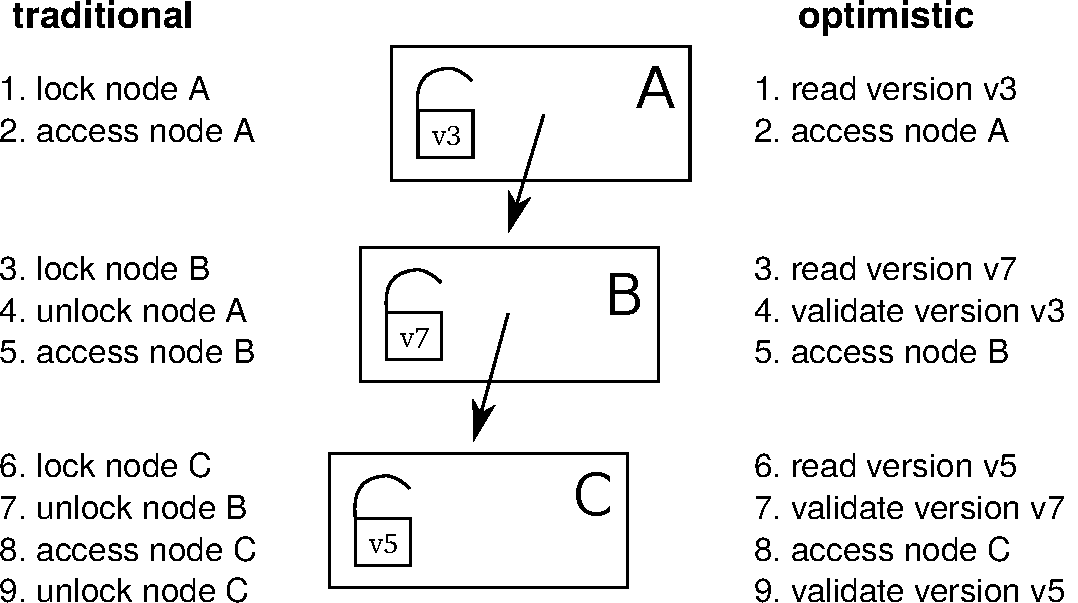
\includegraphics[width=0.65\linewidth]{olcall.pdf}
  \vspace{0.2cm}
  \caption{Comparison of a lookup operation in a 3-level tree using traditional lock coupling (left-hand side) vs.~optimistic lock coupling (right-hand side).}
  \label{fig:olc}
\end{figure}

The traditional and most common lock-based synchronization protocol for B-trees is lock coupling, which interleaves lock acquisitions while holding at most two locks at a time.
If, as we observed earlier, optimistic locks have similar semantics as traditional locks, it is natural to ask whether lock coupling can be combined with optimistic locks.
And indeed the answer is yes: One can almost mechanically translate traditional lock coupling code to optimistic lock coupling code.
This is illustrated in Figure~\ref{fig:olc}, which compares the traversal in a tree of height 3 using traditional and optimistic locks.
As the figure shows, the main difference is that locking is translated to reading the version and that unlocking becomes validation of the previously read version.
This simple change provides efficient lock-free tree traversal without the need to design a complex synchronization protocol.

It is important to emphasize the conceptual simplicity of OLC in comparison to data structures that use custom protocols like the Bw-tree~\cite{DBLP:conf/icde/LevandoskiLS13a}.
To implement lock-free access, the Bw-tree requires an indirection table, delta nodes, complex splitting and merging logic, retry logic, etc.
OLC, on the other hand, can directly be applied to B-trees mostly by adding the appropriate optimistic locking code and without modifying the node layout itself.
Therefore, OpenBw-Tree, an open source implementation of the Bw-tree, requires an order of magnitude more code than a B-tree based on OLC\footnote{Both implementations are available on GitHub: \url{https://github.com/wangziqi2016/index-microbench}}.
Given how difficult it is to develop, validate, and debug lock-free code, simplicity is obviously a major advantage.

\subsection{Correctness Aspects}

\begin{figure}
  % \centering
  %[basicstyle=\normalsize\ttfamily,showstringspaces=false,columns=fullflexible,breaklines=false,breakatwhitespace=true,numbers=none,numberstyle=\small,style=C,keepspaces=true]
\begin{lstlisting}[basicstyle=\ttfamily,language=C++,numbers=left,numberstyle=\small]
std::atomic<BTreeNode*> root;

// search for key in B+tree, returns payload in resultOut
bool lookup(Key key, Value& resultOut) {
   BTreeNode* node = root.load();
   uint64_t nodeVersion = node->readLockOrRestart();
   if (node != root.load()) // make sure the root is still the root
      restart();

   BTreeInner<Key>* parent = nullptr;
   uint64_t parentVersion = 0;

   while (node->isInner()) {
      auto inner = (BTreeInner*)node;

      // unlock parent and make current node the parent
      if (parent)
         parent->readUnlockOrRestart(parentVersion);
      parent = inner;
      parentVersion = nodeVersion;

      // search for next node
      node = inner->findChild(key);
      // validate 'inner' to ensure that 'node' pointer is valid
      inner->checkOrRestart(nodeVersion);
      // now it safe to dereference 'node' pointer (read its version)
      nodeVersion = node->readLockOrRestart();
   }

   // search in leaf and retrieve payload
   auto leaf = (BTreeLeaf*)node;
   bool success = leaf->findValue(key, resultOut);

   // unlock everything
   if (parent)
      parent->readUnlockOrRestart(parentVersion);
   node->readUnlockOrRestart(nodeVersion);

   return success;
}
\end{lstlisting}
  \vspace{0.2cm}
  \caption{B-tree lookup code using OLC. For simplicity, the restart logic is not shown.}
  \label{fig:lookup}
\end{figure}

So far, we have introduced the high-level ideas behind OLC and have stressed its similarity to traditional lock coupling.
Let us now discuss some cases where the close similarity between lock coupling and OLC breaks down.
To make this more concrete, we show the B-tree lookup code in Figure~\ref{fig:lookup}.
In the code, \texttt{readLockOrRestart} reads the lock version and \texttt{readUnlockOrRestart} validates that the read was correct.

One issue with OLC is that any pointer speculatively read from a node may point to invalid memory (if that node is modified concurrently).
Dereferencing such a pointer (e.g., to read its optimistic lock), may cause a segmentation fault or undefined behavior.
In the code shown in Figure~\ref{fig:lookup}, this problem is prevented by the extra check in line 25, which ensures that the read from the node containing the pointer was correct.
Without this additional validation, the code would in line 27 dereference the pointer speculatively read in line 23.
Note that the implementation of \texttt{checkOrRestart} is actually identical to \texttt{readUnlockOrRestart}.
We chose to give it a different name to highlight the fact that this extra check would not be necessary with read/write locks.

Another potential issue with optimistic locks is code that does not terminate.
Code that speculatively accesses a node, like an intra-node binary search, should be written in a way such that it always terminates---even in the presence of concurrent writes.
Otherwise, the validation code that detects the concurrent write will never run.
The binary search of a B-tree, for example, needs to be written in such a way that each comparison makes progress.
For some data structures that do not require loops in the traversal code (like ART) termination is trivially true.

\subsection{Implementation Details}

% implementation, efficiency
To implement an optimistic lock, one can combine the lock and the version counter into a single 64-bit\footnote{Even after subtracting one bit for the lock status, a back-of-the-envelope calculation can show that 63 bits are large enough to never overflow in practice.} word~\cite{artsync}.
A typical read operation will therefore merely consist of reading this version counter atomically.
In C++11 this can be implemented using the \texttt{std::atomic} type.

On x86, atomic reads are cheap because of x86's strong memory order guarantees.
No memory fences are required for sequentially-consistent loads, which are translated (by both GCC and clang) into standard \texttt{MOV} instructions.
Hence, the only effect of \texttt{std::atomic} for loads is preventing instruction re-ordering.
This makes version access and validation cheap.
Acquiring and releasing an optimistic lock in exclusive mode has comparable cost to a traditional lock:
A fairly expensive sequentially-consistent store is needed for acquiring a lock, while a standard \texttt{MOV} suffices for releasing it.
A simple sinlock-based implementation of optimistic locks can be found in the appendix of an earlier paper~\cite{artsync}.

OLC code must be able to handle restarts since validation or lock upgrade can fail due to concurrent writers.
Restarts can easily be implemented by wrapping the data structure operation in a loop (for simplicity not shown in Figure~\ref{fig:lookup}).
Such a loop also enables limiting the number of optimistic retry operations and falling back to pessimistic locking in cases of very heavy contention.
The ability to fall back to traditional locking is a major advantage of OLC in terms of robustness over lock-free approaches, which do not have this option.

In addition to the optimistic shared mode and the exclusive mode, optimistic locks also support a ``shared pessimistic'' mode, which physically acquires the lock in shared mode (allowing multiple concurrent readers but no writers).
This mode is useful for table (or range) scans that touch many tuples on a leaf page (which would otherwise easily abort).
Finally, let us mention that large range scans and table scans, should be broken up into several per-node traversals as is done in the LeanStore~\cite{leanstore} system.

Like all lock-free data structures, but unlike traditional locking and Hardware Transactional Memory~\cite{DBLP:conf/hpca/KarnagelDRLLSL14,DBLP:journals/pvldb/MakreshanskiLS15,htmtkde}, OLC requires care when deleting (and reusing) nodes.
The reason is that a deleting thread can never be sure that a node can be reclaimed because other threads might still be optimistically reading from that node.
Therefore, standard solutions like epoch-based reclamation~\cite{DBLP:conf/sosp/TuZKLM13}, hazard pointers~\cite{DBLP:journals/tpds/Michael04}, or optimized hazard pointers~\cite{DBLP:conf/spaa/BalmauGHZ16} need to be used.
These memory reclamation techniques are, however, largely orthogonal to the synchronization protocol itself.

%-lock-free is not a strong guarantee

\newpage
\section{Evaluation}\label{sec:evaluation}

Let us now experimentally evaluate the overhead and scalability of OLC.
For the experiments, we use an in-memory B+tree implemented in C++11 using templates, which is configured to use nodes of 4096 bytes, random 8 byte keys, and 8 byte payloads.
Based on this B-tree, we compare the following synchronization approaches:
\begin{itemize}
\item an OLC implementation\footnote{An almost identical OLC implementation is available on github: \url{https://github.com/wangziqi2016/index-microbench/tree/master/BTreeOLC}}
\item a variant based on traditional lock coupling and read/write locks
\item the unsynchronized B-tree, which obviously is only correct for read-only workloads but allows measuring the overhead of synchronization
\end{itemize}
Note that earlier work has compared the OLC implementation with a Bw-tree implementation~\cite{buzzword} and other state-of-the-art in-memory index structures.

We use a Haswell EP system with an Intel Xeon E5-2687W v3 CPU, which has 10 cores (20 ``Hyper-Threads'') and 25~MB of L3 cache.
The system is running Ubuntu 18.10 and we use GCC 8.2.0 to compile our code.
The CPU counters are obtained using the Linux perf API\footnote{We use the following convenience wrapper: \url{https://github.com/viktorleis/perfevent}}.

\begin{table}
  \caption{Performance and CPU counters for lookup and insert operations in a B-tree with 100M keys. We perform 100M operations and normalize the CPU counters by that number.}
  \label{tab:overhead}
  \centering
  \begin{tabular}{lrrrrrrr}\toprule
                    &         &        &        & instruc-  & L1     & L3     & branch \\
                    & threads & M op/s & cycles & tions & misses & misses & misses \\\midrule
lookup (no sync.)   & 1       & 1.72   & 2028   & 283     & 39.1   & 14.9   & 16.1   \\
lookup (OLC)        & 1       & 1.65   & 2107   & 370     & 43.9   & 15.1   & 16.7   \\
lookup (lock coup.) & 1       & 1.72   & 2078   & 365     & 42.3   & 16.9   & 15.7   \\\midrule
insert (no sync.)   & 1       & 1.51   & 2286   & 530     & 59.8   & 31.1   & 17.3   \\
insert (OLC)        & 1       & 1.50   & 2303   & 629     & 61.2   & 31.1   & 16.5   \\
insert (lock coup.) & 1       & 1.41   & 2473   & 644     & 61.0   & 31.0   & 17.2   \\\midrule
lookup (no sync.)   & 10      & 15.48  & 2058   & 283     & 38.6   & 15.5   & 16.0   \\
lookup (OLC)        & 10      & 14.60  & 2187   & 370     & 43.8   & 15.8   & 16.8   \\
lookup (lock coup.) & 10      & 5.71   & 5591   & 379     & 54.2   & 17.0   & 14.8   \\\midrule
insert (no sync.)   & 10      & -      & -      & -       & -      & -      & -      \\
insert (OLC)        & 10      & 10.46  & 2940   & 656     & 62.0   & 32.5   & 16.8   \\
insert (lock coup.) & 10      & 7.55   & 4161   & 667     & 75.0   & 28.6   & 16.2   \\
    \bottomrule
\end{tabular}
\end{table}

Table~\ref{tab:overhead} compares the performance and CPU counters for lookup and insert operations in a B-tree with 100M keys.
With {\em single-threaded} execution, we observe that all three approaches have very similar performance.
Adding traditional or optimistic locks to unsynchronized B-tree code results in up to 30\% of additional instructions without affecting single-threaded performance much.

\begin{figure}
  \centering
  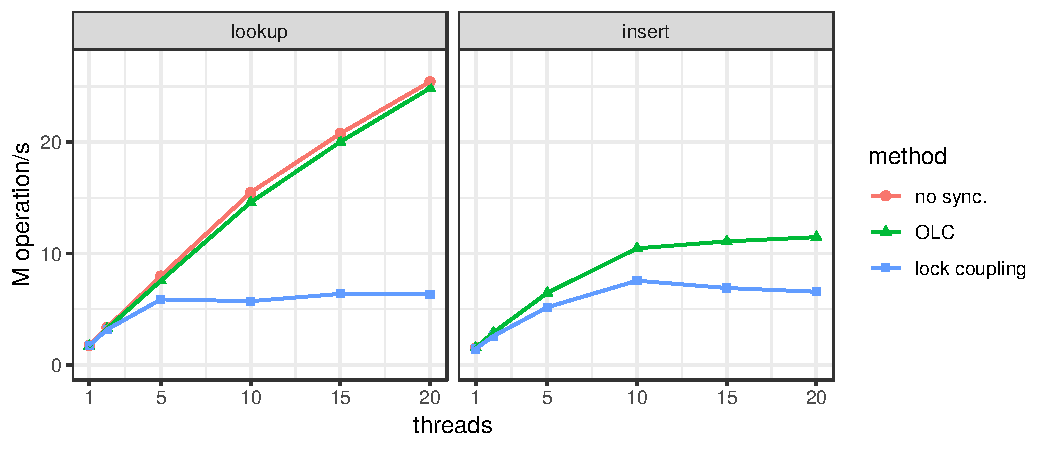
\includegraphics[width=\linewidth]{scale.pdf}
  \vspace{0.2cm}
  \caption{Scalability on 10-core system for B-tree operations (100M values).}
  \label{fig:scale}
\end{figure}

As Figure~\ref{fig:scale} shows, the results change dramatically once we use multiple threads.
For lookup, the scalability of OLC is near-linear up to 20 threads, even though the system has only 10 ``real cores''.
The OLC scalability for insert is also respectable (though not quite as linear because multi-threaded insertion approaches the memory bandwidth of our processor).
The figure also shows that the results of traditional lock coupling with read/write locks are significantly worse than OLC.
With 20 threads, lookup with OLC is 3.9$\times$ faster than traditional lock coupling.

\section{Summary}\label{sec:conc}

Optimistic Lock Coupling (OLC) is an effective synchronization method that combines the simplicity of traditional lock coupling with the superior scalability of lock-free approaches.
OLC is widely applicable and has already been successfully used to synchronize several data structures, including B-trees, binary search trees, and different trie variants.
These features make it highly attractive for modern database systems as well as performance-critical systems software in general.

\begin{thebibliography}{10}

\bibitem{DBLP:conf/spaa/BalmauGHZ16}
O.~Balmau, R.~Guerraoui, M.~Herlihy, and I.~Zablotchi.
\newblock Fast and robust memory reclamation for concurrent data structures.
\newblock In {\em SPAA}, 2016.

\bibitem{DBLP:journals/acta/BayerS77}
R.~Bayer and M.~Schkolnick.
\newblock Concurrency of operations on {B}-trees.
\newblock {\em Acta Informatica}, 9, 1977.

\bibitem{hot}
R.~Binna, E.~Zangerle, M.~Pichl, G.~Specht, and V.~Leis.
\newblock {HOT}: A height optimized trie index for main-memory database
  systems.
\newblock In {\em SIGMOD}, 2018.

\bibitem{DBLP:conf/ppopp/BronsonCCO10}
N.~G. Bronson, J.~Casper, H.~Chafi, and K.~Olukotun.
\newblock A practical concurrent binary search tree.
\newblock In {\em PPOPP}, 2010.

\bibitem{DBLP:conf/vldb/ChaHKK01}
S.~K. Cha, S.~Hwang, K.~Kim, and K.~Kwon.
\newblock Cache-conscious concurrency control of main-memory indexes on
  shared-memory multiprocessor systems.
\newblock In {\em VLDB}, 2001.

\bibitem{intel}
I.~Cutress.
\newblock {Intel} goes for 48-cores: {Cascade-AP} with multi-chip package
  coming soon.
\newblock
  \url{https://www.anandtech.com/show/13535/intel-goes-for-48cores-cascade-ap},
  2018 (accessed January, 2019).

\bibitem{DBLP:conf/cidr/FaleiroA17}
J.~M. Faleiro and D.~J. Abadi.
\newblock Latch-free synchronization in database systems: Silver bullet or
  fool's gold?
\newblock In {\em CIDR}, 2017.

\bibitem{DBLP:journals/ftdb/Graefe11}
G.~Graefe.
\newblock Modern {B}-tree techniques.
\newblock {\em Foundations and Trends in Databases}, 3(4), 2011.

\bibitem{DBLP:conf/hpca/KarnagelDRLLSL14}
T.~Karnagel, R.~Dementiev, R.~Rajwar, K.~Lai, T.~Legler, B.~Schlegel, and
  W.~Lehner.
\newblock Improving in-memory database index performance with
  {Intel}\({}^{\mbox{{\textregistered}}}\) transactional synchronization
  extensions.
\newblock In {\em HPCA}, 2014.

\bibitem{DBLP:journals/tods/LehmanY81}
P.~L. Lehman and S.~B. Yao.
\newblock Efficient locking for concurrent operations on {B}-trees.
\newblock {\em {ACM} Trans. Database Syst.}, 6(4), 1981.

\bibitem{leanstore}
V.~Leis, M.~Haubenschild, A.~Kemper, and T.~Neumann.
\newblock Leanstore: In-memory data management beyond main memory.
\newblock In {\em ICDE}, 2018.

\bibitem{art}
V.~Leis, A.~Kemper, and T.~Neumann.
\newblock The adaptive radix tree: {ARTful} indexing for main-memory databases.
\newblock In {\em ICDE}, 2013.

\bibitem{htmtkde}
V.~Leis, A.~Kemper, and T.~Neumann.
\newblock Scaling {HTM}-supported database transactions to many cores.
\newblock {\em {IEEE} Trans. Knowl. Data Eng.}, 28(2), 2016.

\bibitem{artsync}
V.~Leis, F.~Scheibner, A.~Kemper, and T.~Neumann.
\newblock The {ART} of practical synchronization.
\newblock In {\em DaMoN}, 2016.

\bibitem{DBLP:conf/icde/LevandoskiLS13a}
J.~J. Levandoski, D.~B. Lomet, and S.~Sengupta.
\newblock The {Bw}-tree: A {B}-tree for new hardware platforms.
\newblock In {\em ICDE}, 2013.

\bibitem{DBLP:journals/pvldb/MakreshanskiLS15}
D.~Makreshanski, J.~J. Levandoski, and R.~Stutsman.
\newblock To lock, swap, or elide: On the interplay of hardware transactional
  memory and lock-free indexing.
\newblock {\em {PVLDB}}, 8(11), 2015.

\bibitem{DBLP:dblp_conf/eurosys/MaoKM12}
Y.~Mao, E.~Kohler, and R.~T. Morris.
\newblock Cache craftiness for fast multicore key-value storage.
\newblock In {\em EuroSys}, 2012.

\bibitem{DBLP:journals/tpds/Michael04}
M.~M. Michael.
\newblock Hazard pointers: Safe memory reclamation for lock-free objects.
\newblock {\em {IEEE} Trans. Parallel Distrib. Syst.}, 15(6), 2004.

\bibitem{DBLP:journals/jacm/ShalevS06}
O.~Shalev and N.~Shavit.
\newblock Split-ordered lists: Lock-free extensible hash tables.
\newblock {\em J. {ACM}}, 53(3), 2006.

\bibitem{amd}
A.~Shilov.
\newblock {AMD} previews {EPYC} ‘{Rome}’ processor: Up to 64 {Zen} 2 cores.
\newblock
  \url{https://www.anandtech.com/show/13561/amd-previews-epyc-rome-processor-up-to-64-zen-2-cores},
  2018 (accessed January, 2019).

\bibitem{DBLP:conf/sosp/TuZKLM13}
S.~Tu, W.~Zheng, E.~Kohler, B.~Liskov, and S.~Madden.
\newblock Speedy transactions in multicore in-memory databases.
\newblock In {\em SOSP}, 2013.

\bibitem{buzzword}
Z.~Wang, A.~Pavlo, H.~Lim, V.~Leis, H.~Zhang, M.~Kaminsky, and D.~Andersen.
\newblock Building a {Bw}-tree takes more than just buzz words.
\newblock In {\em SIGMOD}, 2018.

\end{thebibliography}


%\bibliographystyle{abbrv}
%\bibliography{main}

\end{document}

\end{article}
\begin{article}
{Fact Ranking over Large-Scale Knowledge Graphs with Reasoning Embedding Models}
{Hongyu Ren, Ali Mousavi, Anil Pacaci, Shihabur R. Chowdhury, Jason Mohoney,
Ihab F. Ilyas, Yunyao Li, Theodoros Rekatsinas}
\pdfminorversion=5
\documentclass[11pt]{article}
\usepackage{deauthor,times,graphicx,caption,microtype}
\usepackage{hyperref}
\usepackage{listings}
\usepackage{booktabs}

\begin{document}

\title{Optimistic Lock Coupling: A Scalable and Efficient General-Purpose Synchronization Method}

\author{Viktor Leis, Michael Haubenschild\raisebox{0.9ex}{$\ast$}, Thomas Neumann\\ Technische Universit{\"a}t M{\"u}nchen \hspace{0.7cm} Tableau Software\raisebox{0.9ex}{$\ast$} \\ {\{leis,neumann\}{@}in.tum.de} \hspace{0.7cm} {mhaubenschild{@}tableau.com\raisebox{0.9ex}{$\ast$}}}

\maketitle

\begin{abstract}
As the number of cores on commodity processors continues to increase, scalability becomes more and more crucial for overall performance.
Scalable and efficient concurrent data structures are particularly important, as these are often the building blocks of parallel algorithms.
Unfortunately, traditional synchronization techniques based on fine-grained locking have been shown to be unscalable on modern multi-core CPUs.
Lock-free data structures, on the other hand, are extremely difficult to design and often incur significant overhead.

In this work, we make the case for Optimistic Lock Coupling as a practical alternative to both traditional locking and the lock-free approach.
We show that Optimistic Lock Coupling is highly scalable and almost as simple to implement as traditional lock coupling.
Another important advantage is that it is easily applicable to most tree-like data structures.
We therefore argue that Optimistic Lock Coupling, rather than a complex and error-prone custom synchronization protocol, should be the default choice for performance-critical data structures.
\end{abstract}

\section{Introduction}

% more and more cores
Today, Intel's commodity server processors have up to 28 cores and its upcoming microarchitecture will have up to 48 cores per socket~\cite{intel}.
Similarly, AMD currently stands at 32 cores and this number is expected to double in the next generation~\cite{amd}.
Since both platforms support simultaneous multithreading (also known as hyperthreading), affordable commodity servers (with up to two sockets) will soon routinely have between 100 and 200 hardware threads.

% data structure scalability is important
With such a high degree of hardware parallelism, efficient data processing crucially depends on how well concurrent data structures scale.
Internally, database systems use a plethora of data structures like table heaps, internal work queues, and, most importantly, index structures.
Any of these can easily become a scalability (and therefore overall performance) bottleneck on many-core CPUs.

% traditional synchronization: fine-grained locks, slow, cache invalidation
Traditionally, database systems synchronize internal data structures using fine-grained reader/writer locks\footnote{In this work, we focus on data structure synchronization rather than high-level transaction semantics and therefore use the term {\em lock} for what would typically be called {\em latch} in the database literature. We thus follow common computer science (rather than database) terminology.}.
Unfortunately, while fine-grained locking makes lock contention unlikely, it still results in bad scalability because lock acquisition and release require writing to shared memory.
Due to the way cache coherency is implemented on modern multi-core CPUs, these writes cause additional cache misses\footnote{The cache coherency protocol ensures that all copies of a cache line on other cores are invalidated before the write can proceed.} and the cache line containing the lock's internal data becomes a point of physical contention.
As a result, any frequently-accessed lock (e.g., the lock of the root node of a B-tree) severely limits scalability.

% lock-free bw-tree: no more latches, but indirections, extremely complex
Lock-free data structures like the Bw-tree~\cite{DBLP:conf/icde/LevandoskiLS13a} (a lock-free B-tree variant) or the Split-Ordered List~\cite{DBLP:journals/jacm/ShalevS06} (a lock-free hash table) do not acquire any locks and therefore generally scale much better than locking-based approaches (in particular for read-mostly workloads).
However, lock-free synchronization has other downsides:
First, it is very difficult and results in extremely complex and error-prone code (when compared to locking).
Second, because the functionality of atomic primitives provided by the hardware (e.g., atomically compare-and-swap 8 bytes) is limited, complex operations require additional indirections within the data structure.
For example, the Bw-tree requires an indirection table and the Split-Ordered List requires ``dummy nodes'', resulting in overhead due to additional cache misses.

% OLC for the win
In this paper we make the case for {\em Optimistic Lock Coupling (OLC)}, a synchronization method that combines some of the best properties of lock-based and lock-free synchronization.
OLC utilizes a special lock type that can be used in two modes:
The first mode is similar to a traditional mutex and excludes other threads by physically acquiring the underlying lock.
In the second mode, reads can proceed optimistically by validating a version counter that is embedded in the lock (similar to optimistic concurrency control).
The first mode is typically used by writers and the second mode by readers.
Besides this special lock type, OLC is based on the observation that optimistic lock validations can be interleaved/coupled---similar to the pair-wise interleaved lock acquisition of traditional lock coupling.
Hence, the name Optimistic Lock Coupling.

OLC has a number of desirable features:
\begin{itemize}
\item By reducing the number of writes to shared memory locations and thereby avoiding cache invalidations, it {\bf scales well} for most workloads.
\item In comparison to unsynchronized code, it requires few additional CPU instructions making it {\bf efficient}.
\item OLC is {\bf widely applicable} to different data structures. It has already been successfully used for synchronizing binary search trees~\cite{DBLP:conf/ppopp/BronsonCCO10}, tries~\cite{artsync}, trie/B-tree hybrids~\cite{DBLP:dblp_conf/eurosys/MaoKM12}, and B-trees~\cite{buzzword}.
\item In comparison to the lock-free paradigm, it is also {\bf easy to use} and requires few modifications to existing, single-threaded data structures.
\end{itemize}
Despite these positive features and its simplicity, OLC is not yet widely known.
The goal of this paper is therefore to popularize this simple idea and to make a case for it.
We argue that OLC deserves to be widely known.
It is a good default synchronization paradigm---more complex, data structure-specific protocols are seldom beneficial.

The rest of the paper is organized as follows.
Section~\ref{sec:related} discusses related work, tracing the history of OLC and its underlying ideas in the literature.
The core of the paper is Section~\ref{sec:olc}, which describes the ideas behind OLC and how it can be used to synchronize complex data structures.
In Section~\ref{sec:evaluation} we experimentally show that OLC has low overhead and scales well when used to synchronize an in-memory B-tree.
We summarize the paper in Section~\ref{sec:conc}.

\newpage
\section{Related Work}\label{sec:related}

Lock coupling has been proposed as a method for allowing concurrent operations on B-trees in 1977~\cite{DBLP:journals/acta/BayerS77}.
This traditional and still widely-used method, described in detail in Graefe's B-tree survey~\cite{DBLP:journals/ftdb/Graefe11}, is also called ``latch coupling'', ``hand-over-hand locking'', and ``crabbing''.
Because at most two locks are held at-a-time during tree traversal, this technique seemingly allows for a high degree of parallelism---in particular if read/write locks are used to enable inner nodes to be locked in shared mode.
However, as we show in Section~\ref{sec:evaluation}, on modern hardware lock acquisition (even in shared mode) results in suboptimal scalability.

An early alternative from 1981 is a B-tree variant called B-link tree~\cite{DBLP:journals/tods/LehmanY81}, which only holds a single lock at a time.
It is based on the observation that between the release of the parent lock and the acquisition of the child lock, the only ``dangerous'' thing that could have happened is the split of a child node (assuming one does not implement merge operations).
Thus, when a split happens, the key being searched might end up on a neighboring node to the right of the current child node.
A B-link tree traversal therefore detects this condition and, if needed, transparently proceeds to the neighboring node.
Releasing the parent lock early is highly beneficial when the child node needs to be fetched from disk.
For in-memory workloads, however, the B-link tree has the same scalability issues as lock coupling (it acquires just as many locks).

The next major advance, Optimistic Latch-Free Index Traversal (OLFIT)~\cite{DBLP:conf/vldb/ChaHKK01}, was proposed in 2001.
OLFIT introduced the idea of a combined lock/update counter, which we call {\em optimistic lock}. % , for lack of a better name,
Based on these per-node optimistic locks and the synchronization protocol of the B-link tree, OLFIT finally achieves good scalability on parallel processors.
The OLFIT protocol is fairly complex, as it requires both the non-trivial B-link protocol and optimistic locks.
Furthermore, like the B-link tree protocol, it does not support merging nodes, and is specific to B-trees (cannot easily be applied to other data structures).

In the following two decades, the growth of main-memory capacity led to much research into other data structures besides the venerable B-tree.
Particularly relevant for our discussion is Bronson et al.'s~\cite{DBLP:conf/ppopp/BronsonCCO10} concurrent binary search tree, which is based on optimistic version validation and has a sophisticated, data structure-specific synchronization protocol.
To the best of our knowledge, this 2010 paper is the first that, as part of its protocol, interleaves version validation across nodes---rather than validating each node separately like OLFIT.
In that paper, this idea is called ``hand-over-hand, optimistic validation'', while we prefer the term Optimistic Lock Coupling to highlight the close resemblance to traditional lock coupling.
Similarly, Mao et al.'s~\cite{DBLP:dblp_conf/eurosys/MaoKM12} Masstree (a concurrent hybrid trie/B-tree) is also based on the same ideas, but again uses them as part of a more complex protocol.

The Adaptive Radix Tree (ART)~\cite{art} is another recent in-memory data structure, which we proposed in 2013.
In contrast to the two data structures just mentioned, it was originally designed with single-threaded performance in mind without supporting concurrency.
To add support for concurrency, we initially started designing a custom protocol called Read-Optimized Write Exclusion (ROWEX)~\cite{artsync}, which turned out to be non-trivial and requires modifications of the underlying data structure\footnote{Note that ROWEX is already easier to apply to existing data structures than the lock-free approach. The difficulty depends on the data structure. Applying ROWEX is hard for B-trees with sorted keys and fairly easy for copy-on-write data structures like the Height Optimized Trie~\cite{hot}---with ART being somewhere in the middle.}.
However, fairly late in the project, we also realized, that OLC {\em alone} (rather than as part of a more complex protocol) is sufficient to synchronize ART.
No other changes to the data structure were necessary.
Both approaches were published and experimentally evaluated in a followup paper~\cite{artsync}, which shows that, despite its simplicity, OLC is efficient, scalable, and generally outperforms ROWEX.

Similar results were recently published regarding B-trees~\cite{buzzword}.
In this experimental study a simple OLC-based synchronization outperformed the Bw-tree~\cite{DBLP:conf/icde/LevandoskiLS13a}, a complex lock-free synchronization approach.
Another recent paper shows that for write-intensive workloads, locking often performs better than lock-free synchronization~\cite{DBLP:conf/cidr/FaleiroA17}.
These experiences indicate that OLC is a general-purpose synchronization paradigm and motivate the current paper.

%foster b-tree\cite{DBLP:journals/tods/GraefeKK12}
%Shasha theory~\cite{DBLP:journals/tods/ShashaG88}

\section{Optimistic Lock Coupling}\label{sec:olc}

% locks suck
The standard technique for inter-thread synchronization is mutual exclusion using fine-grained locks.
In a B-tree, for example, every node usually has its own associated lock, which is acquired before accessing that node.
The problem of locking on modern multi- and many-core processors is that lock acquisition and release require writing to the shared memory location that implements the lock.
This write causes exclusive ownership of the underlying cache line and invalidates copies of it on all other processor cores.
For hierarchical, tree-like data structures, the lock of the root node becomes a point of physical contention---even in read-only workloads and even when read/write locks are used.
Depending on the specific data structure, number of cores, cache coherency protocol implementation, cache topology, whether Non-Uniform Memory Access (NUMA) is used, locking can even result in multi-threaded performance that is worse than single-threaded execution.

% in b-trees this happens very much
The inherent pessimism of locking is particularly unfortunate for B-trees:
Despite the fact that logical modifications of the root node are very infrequent, every B-tree operation must lock the root node during tree traversal\footnote{To a lesser extent this obviously applies to all inner nodes, not just the root.}.
Even the vast majority of update operations (with the exception of splits and merges), only modify a single leaf node.
These observations indicate that a more optimistic approach, which does not require locking inner nodes, would be very beneficial for B-trees.

\subsection{Optimistic Locks}

% optimism to the rescue
As the name indicates, optimistic locks try to solve the scalability issues of traditional locks using an optimistic approach.
Instead of always physically acquiring locks, even for nodes that are unlikely to be modified simultaneously, after-the-fact validation is used to detect conflicts.
This is done by augmenting each lock with a version/update counter that is incremented on every modification.
Using this version counter, readers can optimistically proceed before validating that the version did not change to ensure that the read was safe.
If validation fails, the operation is restarted.

% details on opt locks
Using optimistic locks, a read-only node access (i.e., the majority of all operations in a B-tree) does not acquire the lock and does not increment the version counter.
Instead, it performs the following steps:
\begin{enumerate}
\item read lock version (restart if lock is not free)
\item access node
\item read the version again and validate that it has not changed in the meantime
\end{enumerate}
If the last step (the validation) fails, the operation has to be restarted.
Write operations, on the other hand, are more similar to traditional locking:
\begin{enumerate}
\item acquire lock (wait if necessary)
\item access/write to node
\item increment version and unlock node
\end{enumerate}
Writes can therefore protect a node from other writes.

% similar to locks
As we observed in an earlier paper~\cite{artsync}, because of similar semantics, optimistic locks can be hidden behind an API very similar to traditional read/write locks.
Both approaches have an exclusive lock mode, and acquiring a traditional lock in shared mode is analogous to optimistic version validation.
Furthermore, like with some implementations of traditional read/write locks, optimistic locks allow upgrading a shared lock to an exclusive lock.
Lock upgrades are, for example, used to avoid most B-tree update operations from having to lock inner nodes.
In our experience, the close resemblance of optimistic and traditional locks simplifies the reasoning about optimistic locks;
one can apply similar thinking as in traditional lock-based protocols.

\subsection{Lock Coupling with Optimistic Locks}

\begin{figure}
  \centering
  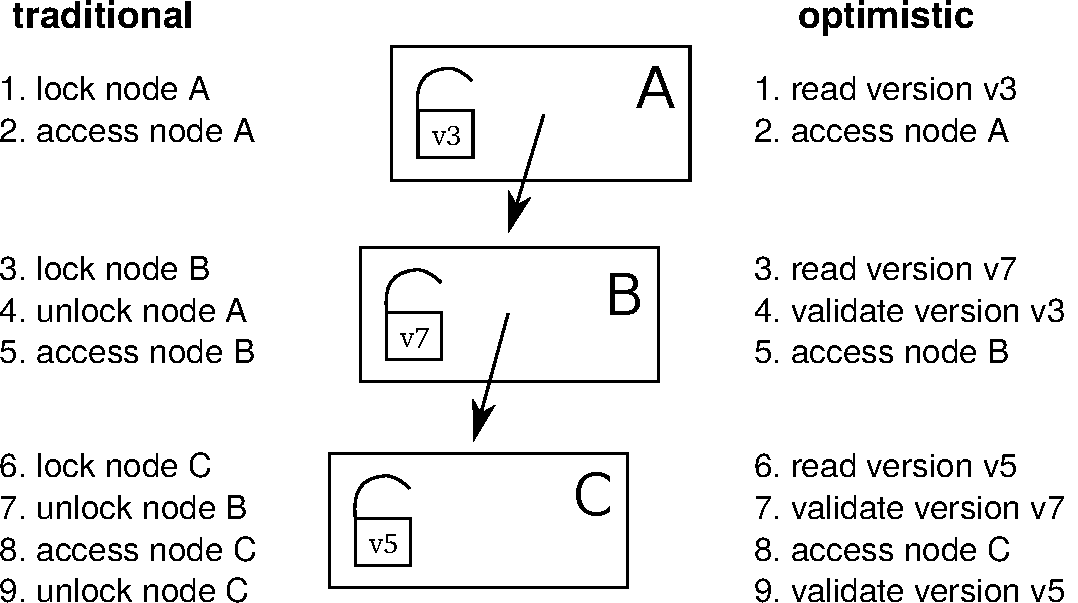
\includegraphics[width=0.65\linewidth]{olcall.pdf}
  \vspace{0.2cm}
  \caption{Comparison of a lookup operation in a 3-level tree using traditional lock coupling (left-hand side) vs.~optimistic lock coupling (right-hand side).}
  \label{fig:olc}
\end{figure}

The traditional and most common lock-based synchronization protocol for B-trees is lock coupling, which interleaves lock acquisitions while holding at most two locks at a time.
If, as we observed earlier, optimistic locks have similar semantics as traditional locks, it is natural to ask whether lock coupling can be combined with optimistic locks.
And indeed the answer is yes: One can almost mechanically translate traditional lock coupling code to optimistic lock coupling code.
This is illustrated in Figure~\ref{fig:olc}, which compares the traversal in a tree of height 3 using traditional and optimistic locks.
As the figure shows, the main difference is that locking is translated to reading the version and that unlocking becomes validation of the previously read version.
This simple change provides efficient lock-free tree traversal without the need to design a complex synchronization protocol.

It is important to emphasize the conceptual simplicity of OLC in comparison to data structures that use custom protocols like the Bw-tree~\cite{DBLP:conf/icde/LevandoskiLS13a}.
To implement lock-free access, the Bw-tree requires an indirection table, delta nodes, complex splitting and merging logic, retry logic, etc.
OLC, on the other hand, can directly be applied to B-trees mostly by adding the appropriate optimistic locking code and without modifying the node layout itself.
Therefore, OpenBw-Tree, an open source implementation of the Bw-tree, requires an order of magnitude more code than a B-tree based on OLC\footnote{Both implementations are available on GitHub: \url{https://github.com/wangziqi2016/index-microbench}}.
Given how difficult it is to develop, validate, and debug lock-free code, simplicity is obviously a major advantage.

\subsection{Correctness Aspects}

\begin{figure}
  % \centering
  %[basicstyle=\normalsize\ttfamily,showstringspaces=false,columns=fullflexible,breaklines=false,breakatwhitespace=true,numbers=none,numberstyle=\small,style=C,keepspaces=true]
\begin{lstlisting}[basicstyle=\ttfamily,language=C++,numbers=left,numberstyle=\small]
std::atomic<BTreeNode*> root;

// search for key in B+tree, returns payload in resultOut
bool lookup(Key key, Value& resultOut) {
   BTreeNode* node = root.load();
   uint64_t nodeVersion = node->readLockOrRestart();
   if (node != root.load()) // make sure the root is still the root
      restart();

   BTreeInner<Key>* parent = nullptr;
   uint64_t parentVersion = 0;

   while (node->isInner()) {
      auto inner = (BTreeInner*)node;

      // unlock parent and make current node the parent
      if (parent)
         parent->readUnlockOrRestart(parentVersion);
      parent = inner;
      parentVersion = nodeVersion;

      // search for next node
      node = inner->findChild(key);
      // validate 'inner' to ensure that 'node' pointer is valid
      inner->checkOrRestart(nodeVersion);
      // now it safe to dereference 'node' pointer (read its version)
      nodeVersion = node->readLockOrRestart();
   }

   // search in leaf and retrieve payload
   auto leaf = (BTreeLeaf*)node;
   bool success = leaf->findValue(key, resultOut);

   // unlock everything
   if (parent)
      parent->readUnlockOrRestart(parentVersion);
   node->readUnlockOrRestart(nodeVersion);

   return success;
}
\end{lstlisting}
  \vspace{0.2cm}
  \caption{B-tree lookup code using OLC. For simplicity, the restart logic is not shown.}
  \label{fig:lookup}
\end{figure}

So far, we have introduced the high-level ideas behind OLC and have stressed its similarity to traditional lock coupling.
Let us now discuss some cases where the close similarity between lock coupling and OLC breaks down.
To make this more concrete, we show the B-tree lookup code in Figure~\ref{fig:lookup}.
In the code, \texttt{readLockOrRestart} reads the lock version and \texttt{readUnlockOrRestart} validates that the read was correct.

One issue with OLC is that any pointer speculatively read from a node may point to invalid memory (if that node is modified concurrently).
Dereferencing such a pointer (e.g., to read its optimistic lock), may cause a segmentation fault or undefined behavior.
In the code shown in Figure~\ref{fig:lookup}, this problem is prevented by the extra check in line 25, which ensures that the read from the node containing the pointer was correct.
Without this additional validation, the code would in line 27 dereference the pointer speculatively read in line 23.
Note that the implementation of \texttt{checkOrRestart} is actually identical to \texttt{readUnlockOrRestart}.
We chose to give it a different name to highlight the fact that this extra check would not be necessary with read/write locks.

Another potential issue with optimistic locks is code that does not terminate.
Code that speculatively accesses a node, like an intra-node binary search, should be written in a way such that it always terminates---even in the presence of concurrent writes.
Otherwise, the validation code that detects the concurrent write will never run.
The binary search of a B-tree, for example, needs to be written in such a way that each comparison makes progress.
For some data structures that do not require loops in the traversal code (like ART) termination is trivially true.

\subsection{Implementation Details}

% implementation, efficiency
To implement an optimistic lock, one can combine the lock and the version counter into a single 64-bit\footnote{Even after subtracting one bit for the lock status, a back-of-the-envelope calculation can show that 63 bits are large enough to never overflow in practice.} word~\cite{artsync}.
A typical read operation will therefore merely consist of reading this version counter atomically.
In C++11 this can be implemented using the \texttt{std::atomic} type.

On x86, atomic reads are cheap because of x86's strong memory order guarantees.
No memory fences are required for sequentially-consistent loads, which are translated (by both GCC and clang) into standard \texttt{MOV} instructions.
Hence, the only effect of \texttt{std::atomic} for loads is preventing instruction re-ordering.
This makes version access and validation cheap.
Acquiring and releasing an optimistic lock in exclusive mode has comparable cost to a traditional lock:
A fairly expensive sequentially-consistent store is needed for acquiring a lock, while a standard \texttt{MOV} suffices for releasing it.
A simple sinlock-based implementation of optimistic locks can be found in the appendix of an earlier paper~\cite{artsync}.

OLC code must be able to handle restarts since validation or lock upgrade can fail due to concurrent writers.
Restarts can easily be implemented by wrapping the data structure operation in a loop (for simplicity not shown in Figure~\ref{fig:lookup}).
Such a loop also enables limiting the number of optimistic retry operations and falling back to pessimistic locking in cases of very heavy contention.
The ability to fall back to traditional locking is a major advantage of OLC in terms of robustness over lock-free approaches, which do not have this option.

In addition to the optimistic shared mode and the exclusive mode, optimistic locks also support a ``shared pessimistic'' mode, which physically acquires the lock in shared mode (allowing multiple concurrent readers but no writers).
This mode is useful for table (or range) scans that touch many tuples on a leaf page (which would otherwise easily abort).
Finally, let us mention that large range scans and table scans, should be broken up into several per-node traversals as is done in the LeanStore~\cite{leanstore} system.

Like all lock-free data structures, but unlike traditional locking and Hardware Transactional Memory~\cite{DBLP:conf/hpca/KarnagelDRLLSL14,DBLP:journals/pvldb/MakreshanskiLS15,htmtkde}, OLC requires care when deleting (and reusing) nodes.
The reason is that a deleting thread can never be sure that a node can be reclaimed because other threads might still be optimistically reading from that node.
Therefore, standard solutions like epoch-based reclamation~\cite{DBLP:conf/sosp/TuZKLM13}, hazard pointers~\cite{DBLP:journals/tpds/Michael04}, or optimized hazard pointers~\cite{DBLP:conf/spaa/BalmauGHZ16} need to be used.
These memory reclamation techniques are, however, largely orthogonal to the synchronization protocol itself.

%-lock-free is not a strong guarantee

\newpage
\section{Evaluation}\label{sec:evaluation}

Let us now experimentally evaluate the overhead and scalability of OLC.
For the experiments, we use an in-memory B+tree implemented in C++11 using templates, which is configured to use nodes of 4096 bytes, random 8 byte keys, and 8 byte payloads.
Based on this B-tree, we compare the following synchronization approaches:
\begin{itemize}
\item an OLC implementation\footnote{An almost identical OLC implementation is available on github: \url{https://github.com/wangziqi2016/index-microbench/tree/master/BTreeOLC}}
\item a variant based on traditional lock coupling and read/write locks
\item the unsynchronized B-tree, which obviously is only correct for read-only workloads but allows measuring the overhead of synchronization
\end{itemize}
Note that earlier work has compared the OLC implementation with a Bw-tree implementation~\cite{buzzword} and other state-of-the-art in-memory index structures.

We use a Haswell EP system with an Intel Xeon E5-2687W v3 CPU, which has 10 cores (20 ``Hyper-Threads'') and 25~MB of L3 cache.
The system is running Ubuntu 18.10 and we use GCC 8.2.0 to compile our code.
The CPU counters are obtained using the Linux perf API\footnote{We use the following convenience wrapper: \url{https://github.com/viktorleis/perfevent}}.

\begin{table}
  \caption{Performance and CPU counters for lookup and insert operations in a B-tree with 100M keys. We perform 100M operations and normalize the CPU counters by that number.}
  \label{tab:overhead}
  \centering
  \begin{tabular}{lrrrrrrr}\toprule
                    &         &        &        & instruc-  & L1     & L3     & branch \\
                    & threads & M op/s & cycles & tions & misses & misses & misses \\\midrule
lookup (no sync.)   & 1       & 1.72   & 2028   & 283     & 39.1   & 14.9   & 16.1   \\
lookup (OLC)        & 1       & 1.65   & 2107   & 370     & 43.9   & 15.1   & 16.7   \\
lookup (lock coup.) & 1       & 1.72   & 2078   & 365     & 42.3   & 16.9   & 15.7   \\\midrule
insert (no sync.)   & 1       & 1.51   & 2286   & 530     & 59.8   & 31.1   & 17.3   \\
insert (OLC)        & 1       & 1.50   & 2303   & 629     & 61.2   & 31.1   & 16.5   \\
insert (lock coup.) & 1       & 1.41   & 2473   & 644     & 61.0   & 31.0   & 17.2   \\\midrule
lookup (no sync.)   & 10      & 15.48  & 2058   & 283     & 38.6   & 15.5   & 16.0   \\
lookup (OLC)        & 10      & 14.60  & 2187   & 370     & 43.8   & 15.8   & 16.8   \\
lookup (lock coup.) & 10      & 5.71   & 5591   & 379     & 54.2   & 17.0   & 14.8   \\\midrule
insert (no sync.)   & 10      & -      & -      & -       & -      & -      & -      \\
insert (OLC)        & 10      & 10.46  & 2940   & 656     & 62.0   & 32.5   & 16.8   \\
insert (lock coup.) & 10      & 7.55   & 4161   & 667     & 75.0   & 28.6   & 16.2   \\
    \bottomrule
\end{tabular}
\end{table}

Table~\ref{tab:overhead} compares the performance and CPU counters for lookup and insert operations in a B-tree with 100M keys.
With {\em single-threaded} execution, we observe that all three approaches have very similar performance.
Adding traditional or optimistic locks to unsynchronized B-tree code results in up to 30\% of additional instructions without affecting single-threaded performance much.

\begin{figure}
  \centering
  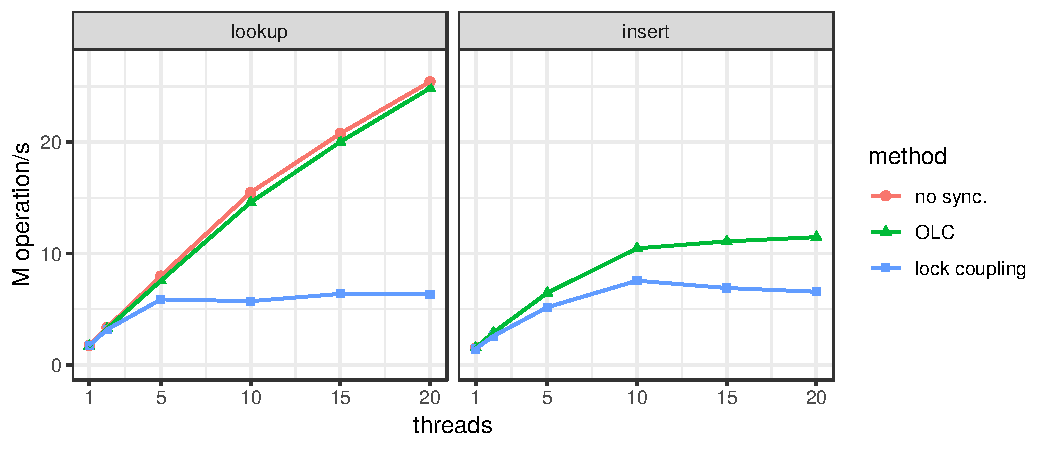
\includegraphics[width=\linewidth]{scale.pdf}
  \vspace{0.2cm}
  \caption{Scalability on 10-core system for B-tree operations (100M values).}
  \label{fig:scale}
\end{figure}

As Figure~\ref{fig:scale} shows, the results change dramatically once we use multiple threads.
For lookup, the scalability of OLC is near-linear up to 20 threads, even though the system has only 10 ``real cores''.
The OLC scalability for insert is also respectable (though not quite as linear because multi-threaded insertion approaches the memory bandwidth of our processor).
The figure also shows that the results of traditional lock coupling with read/write locks are significantly worse than OLC.
With 20 threads, lookup with OLC is 3.9$\times$ faster than traditional lock coupling.

\section{Summary}\label{sec:conc}

Optimistic Lock Coupling (OLC) is an effective synchronization method that combines the simplicity of traditional lock coupling with the superior scalability of lock-free approaches.
OLC is widely applicable and has already been successfully used to synchronize several data structures, including B-trees, binary search trees, and different trie variants.
These features make it highly attractive for modern database systems as well as performance-critical systems software in general.

\begin{thebibliography}{10}

\bibitem{DBLP:conf/spaa/BalmauGHZ16}
O.~Balmau, R.~Guerraoui, M.~Herlihy, and I.~Zablotchi.
\newblock Fast and robust memory reclamation for concurrent data structures.
\newblock In {\em SPAA}, 2016.

\bibitem{DBLP:journals/acta/BayerS77}
R.~Bayer and M.~Schkolnick.
\newblock Concurrency of operations on {B}-trees.
\newblock {\em Acta Informatica}, 9, 1977.

\bibitem{hot}
R.~Binna, E.~Zangerle, M.~Pichl, G.~Specht, and V.~Leis.
\newblock {HOT}: A height optimized trie index for main-memory database
  systems.
\newblock In {\em SIGMOD}, 2018.

\bibitem{DBLP:conf/ppopp/BronsonCCO10}
N.~G. Bronson, J.~Casper, H.~Chafi, and K.~Olukotun.
\newblock A practical concurrent binary search tree.
\newblock In {\em PPOPP}, 2010.

\bibitem{DBLP:conf/vldb/ChaHKK01}
S.~K. Cha, S.~Hwang, K.~Kim, and K.~Kwon.
\newblock Cache-conscious concurrency control of main-memory indexes on
  shared-memory multiprocessor systems.
\newblock In {\em VLDB}, 2001.

\bibitem{intel}
I.~Cutress.
\newblock {Intel} goes for 48-cores: {Cascade-AP} with multi-chip package
  coming soon.
\newblock
  \url{https://www.anandtech.com/show/13535/intel-goes-for-48cores-cascade-ap},
  2018 (accessed January, 2019).

\bibitem{DBLP:conf/cidr/FaleiroA17}
J.~M. Faleiro and D.~J. Abadi.
\newblock Latch-free synchronization in database systems: Silver bullet or
  fool's gold?
\newblock In {\em CIDR}, 2017.

\bibitem{DBLP:journals/ftdb/Graefe11}
G.~Graefe.
\newblock Modern {B}-tree techniques.
\newblock {\em Foundations and Trends in Databases}, 3(4), 2011.

\bibitem{DBLP:conf/hpca/KarnagelDRLLSL14}
T.~Karnagel, R.~Dementiev, R.~Rajwar, K.~Lai, T.~Legler, B.~Schlegel, and
  W.~Lehner.
\newblock Improving in-memory database index performance with
  {Intel}\({}^{\mbox{{\textregistered}}}\) transactional synchronization
  extensions.
\newblock In {\em HPCA}, 2014.

\bibitem{DBLP:journals/tods/LehmanY81}
P.~L. Lehman and S.~B. Yao.
\newblock Efficient locking for concurrent operations on {B}-trees.
\newblock {\em {ACM} Trans. Database Syst.}, 6(4), 1981.

\bibitem{leanstore}
V.~Leis, M.~Haubenschild, A.~Kemper, and T.~Neumann.
\newblock Leanstore: In-memory data management beyond main memory.
\newblock In {\em ICDE}, 2018.

\bibitem{art}
V.~Leis, A.~Kemper, and T.~Neumann.
\newblock The adaptive radix tree: {ARTful} indexing for main-memory databases.
\newblock In {\em ICDE}, 2013.

\bibitem{htmtkde}
V.~Leis, A.~Kemper, and T.~Neumann.
\newblock Scaling {HTM}-supported database transactions to many cores.
\newblock {\em {IEEE} Trans. Knowl. Data Eng.}, 28(2), 2016.

\bibitem{artsync}
V.~Leis, F.~Scheibner, A.~Kemper, and T.~Neumann.
\newblock The {ART} of practical synchronization.
\newblock In {\em DaMoN}, 2016.

\bibitem{DBLP:conf/icde/LevandoskiLS13a}
J.~J. Levandoski, D.~B. Lomet, and S.~Sengupta.
\newblock The {Bw}-tree: A {B}-tree for new hardware platforms.
\newblock In {\em ICDE}, 2013.

\bibitem{DBLP:journals/pvldb/MakreshanskiLS15}
D.~Makreshanski, J.~J. Levandoski, and R.~Stutsman.
\newblock To lock, swap, or elide: On the interplay of hardware transactional
  memory and lock-free indexing.
\newblock {\em {PVLDB}}, 8(11), 2015.

\bibitem{DBLP:dblp_conf/eurosys/MaoKM12}
Y.~Mao, E.~Kohler, and R.~T. Morris.
\newblock Cache craftiness for fast multicore key-value storage.
\newblock In {\em EuroSys}, 2012.

\bibitem{DBLP:journals/tpds/Michael04}
M.~M. Michael.
\newblock Hazard pointers: Safe memory reclamation for lock-free objects.
\newblock {\em {IEEE} Trans. Parallel Distrib. Syst.}, 15(6), 2004.

\bibitem{DBLP:journals/jacm/ShalevS06}
O.~Shalev and N.~Shavit.
\newblock Split-ordered lists: Lock-free extensible hash tables.
\newblock {\em J. {ACM}}, 53(3), 2006.

\bibitem{amd}
A.~Shilov.
\newblock {AMD} previews {EPYC} ‘{Rome}’ processor: Up to 64 {Zen} 2 cores.
\newblock
  \url{https://www.anandtech.com/show/13561/amd-previews-epyc-rome-processor-up-to-64-zen-2-cores},
  2018 (accessed January, 2019).

\bibitem{DBLP:conf/sosp/TuZKLM13}
S.~Tu, W.~Zheng, E.~Kohler, B.~Liskov, and S.~Madden.
\newblock Speedy transactions in multicore in-memory databases.
\newblock In {\em SOSP}, 2013.

\bibitem{buzzword}
Z.~Wang, A.~Pavlo, H.~Lim, V.~Leis, H.~Zhang, M.~Kaminsky, and D.~Andersen.
\newblock Building a {Bw}-tree takes more than just buzz words.
\newblock In {\em SIGMOD}, 2018.

\end{thebibliography}


%\bibliographystyle{abbrv}
%\bibliography{main}

\end{document}

\end{article}
\begin{article}
{Graph Data Augmentation for Graph Machine Learning: A Survey}
{Tong Zhao, Wei Jin, Yozen Liu, Yingheng Wang, Gang Liu, Stephan Günnemann, Neil Shah, Meng Jiang}
\pdfminorversion=5
\documentclass[11pt]{article}
\usepackage{deauthor,times,graphicx,caption,microtype}
\usepackage{hyperref}
\usepackage{listings}
\usepackage{booktabs}

\begin{document}

\title{Optimistic Lock Coupling: A Scalable and Efficient General-Purpose Synchronization Method}

\author{Viktor Leis, Michael Haubenschild\raisebox{0.9ex}{$\ast$}, Thomas Neumann\\ Technische Universit{\"a}t M{\"u}nchen \hspace{0.7cm} Tableau Software\raisebox{0.9ex}{$\ast$} \\ {\{leis,neumann\}{@}in.tum.de} \hspace{0.7cm} {mhaubenschild{@}tableau.com\raisebox{0.9ex}{$\ast$}}}

\maketitle

\begin{abstract}
As the number of cores on commodity processors continues to increase, scalability becomes more and more crucial for overall performance.
Scalable and efficient concurrent data structures are particularly important, as these are often the building blocks of parallel algorithms.
Unfortunately, traditional synchronization techniques based on fine-grained locking have been shown to be unscalable on modern multi-core CPUs.
Lock-free data structures, on the other hand, are extremely difficult to design and often incur significant overhead.

In this work, we make the case for Optimistic Lock Coupling as a practical alternative to both traditional locking and the lock-free approach.
We show that Optimistic Lock Coupling is highly scalable and almost as simple to implement as traditional lock coupling.
Another important advantage is that it is easily applicable to most tree-like data structures.
We therefore argue that Optimistic Lock Coupling, rather than a complex and error-prone custom synchronization protocol, should be the default choice for performance-critical data structures.
\end{abstract}

\section{Introduction}

% more and more cores
Today, Intel's commodity server processors have up to 28 cores and its upcoming microarchitecture will have up to 48 cores per socket~\cite{intel}.
Similarly, AMD currently stands at 32 cores and this number is expected to double in the next generation~\cite{amd}.
Since both platforms support simultaneous multithreading (also known as hyperthreading), affordable commodity servers (with up to two sockets) will soon routinely have between 100 and 200 hardware threads.

% data structure scalability is important
With such a high degree of hardware parallelism, efficient data processing crucially depends on how well concurrent data structures scale.
Internally, database systems use a plethora of data structures like table heaps, internal work queues, and, most importantly, index structures.
Any of these can easily become a scalability (and therefore overall performance) bottleneck on many-core CPUs.

% traditional synchronization: fine-grained locks, slow, cache invalidation
Traditionally, database systems synchronize internal data structures using fine-grained reader/writer locks\footnote{In this work, we focus on data structure synchronization rather than high-level transaction semantics and therefore use the term {\em lock} for what would typically be called {\em latch} in the database literature. We thus follow common computer science (rather than database) terminology.}.
Unfortunately, while fine-grained locking makes lock contention unlikely, it still results in bad scalability because lock acquisition and release require writing to shared memory.
Due to the way cache coherency is implemented on modern multi-core CPUs, these writes cause additional cache misses\footnote{The cache coherency protocol ensures that all copies of a cache line on other cores are invalidated before the write can proceed.} and the cache line containing the lock's internal data becomes a point of physical contention.
As a result, any frequently-accessed lock (e.g., the lock of the root node of a B-tree) severely limits scalability.

% lock-free bw-tree: no more latches, but indirections, extremely complex
Lock-free data structures like the Bw-tree~\cite{DBLP:conf/icde/LevandoskiLS13a} (a lock-free B-tree variant) or the Split-Ordered List~\cite{DBLP:journals/jacm/ShalevS06} (a lock-free hash table) do not acquire any locks and therefore generally scale much better than locking-based approaches (in particular for read-mostly workloads).
However, lock-free synchronization has other downsides:
First, it is very difficult and results in extremely complex and error-prone code (when compared to locking).
Second, because the functionality of atomic primitives provided by the hardware (e.g., atomically compare-and-swap 8 bytes) is limited, complex operations require additional indirections within the data structure.
For example, the Bw-tree requires an indirection table and the Split-Ordered List requires ``dummy nodes'', resulting in overhead due to additional cache misses.

% OLC for the win
In this paper we make the case for {\em Optimistic Lock Coupling (OLC)}, a synchronization method that combines some of the best properties of lock-based and lock-free synchronization.
OLC utilizes a special lock type that can be used in two modes:
The first mode is similar to a traditional mutex and excludes other threads by physically acquiring the underlying lock.
In the second mode, reads can proceed optimistically by validating a version counter that is embedded in the lock (similar to optimistic concurrency control).
The first mode is typically used by writers and the second mode by readers.
Besides this special lock type, OLC is based on the observation that optimistic lock validations can be interleaved/coupled---similar to the pair-wise interleaved lock acquisition of traditional lock coupling.
Hence, the name Optimistic Lock Coupling.

OLC has a number of desirable features:
\begin{itemize}
\item By reducing the number of writes to shared memory locations and thereby avoiding cache invalidations, it {\bf scales well} for most workloads.
\item In comparison to unsynchronized code, it requires few additional CPU instructions making it {\bf efficient}.
\item OLC is {\bf widely applicable} to different data structures. It has already been successfully used for synchronizing binary search trees~\cite{DBLP:conf/ppopp/BronsonCCO10}, tries~\cite{artsync}, trie/B-tree hybrids~\cite{DBLP:dblp_conf/eurosys/MaoKM12}, and B-trees~\cite{buzzword}.
\item In comparison to the lock-free paradigm, it is also {\bf easy to use} and requires few modifications to existing, single-threaded data structures.
\end{itemize}
Despite these positive features and its simplicity, OLC is not yet widely known.
The goal of this paper is therefore to popularize this simple idea and to make a case for it.
We argue that OLC deserves to be widely known.
It is a good default synchronization paradigm---more complex, data structure-specific protocols are seldom beneficial.

The rest of the paper is organized as follows.
Section~\ref{sec:related} discusses related work, tracing the history of OLC and its underlying ideas in the literature.
The core of the paper is Section~\ref{sec:olc}, which describes the ideas behind OLC and how it can be used to synchronize complex data structures.
In Section~\ref{sec:evaluation} we experimentally show that OLC has low overhead and scales well when used to synchronize an in-memory B-tree.
We summarize the paper in Section~\ref{sec:conc}.

\newpage
\section{Related Work}\label{sec:related}

Lock coupling has been proposed as a method for allowing concurrent operations on B-trees in 1977~\cite{DBLP:journals/acta/BayerS77}.
This traditional and still widely-used method, described in detail in Graefe's B-tree survey~\cite{DBLP:journals/ftdb/Graefe11}, is also called ``latch coupling'', ``hand-over-hand locking'', and ``crabbing''.
Because at most two locks are held at-a-time during tree traversal, this technique seemingly allows for a high degree of parallelism---in particular if read/write locks are used to enable inner nodes to be locked in shared mode.
However, as we show in Section~\ref{sec:evaluation}, on modern hardware lock acquisition (even in shared mode) results in suboptimal scalability.

An early alternative from 1981 is a B-tree variant called B-link tree~\cite{DBLP:journals/tods/LehmanY81}, which only holds a single lock at a time.
It is based on the observation that between the release of the parent lock and the acquisition of the child lock, the only ``dangerous'' thing that could have happened is the split of a child node (assuming one does not implement merge operations).
Thus, when a split happens, the key being searched might end up on a neighboring node to the right of the current child node.
A B-link tree traversal therefore detects this condition and, if needed, transparently proceeds to the neighboring node.
Releasing the parent lock early is highly beneficial when the child node needs to be fetched from disk.
For in-memory workloads, however, the B-link tree has the same scalability issues as lock coupling (it acquires just as many locks).

The next major advance, Optimistic Latch-Free Index Traversal (OLFIT)~\cite{DBLP:conf/vldb/ChaHKK01}, was proposed in 2001.
OLFIT introduced the idea of a combined lock/update counter, which we call {\em optimistic lock}. % , for lack of a better name,
Based on these per-node optimistic locks and the synchronization protocol of the B-link tree, OLFIT finally achieves good scalability on parallel processors.
The OLFIT protocol is fairly complex, as it requires both the non-trivial B-link protocol and optimistic locks.
Furthermore, like the B-link tree protocol, it does not support merging nodes, and is specific to B-trees (cannot easily be applied to other data structures).

In the following two decades, the growth of main-memory capacity led to much research into other data structures besides the venerable B-tree.
Particularly relevant for our discussion is Bronson et al.'s~\cite{DBLP:conf/ppopp/BronsonCCO10} concurrent binary search tree, which is based on optimistic version validation and has a sophisticated, data structure-specific synchronization protocol.
To the best of our knowledge, this 2010 paper is the first that, as part of its protocol, interleaves version validation across nodes---rather than validating each node separately like OLFIT.
In that paper, this idea is called ``hand-over-hand, optimistic validation'', while we prefer the term Optimistic Lock Coupling to highlight the close resemblance to traditional lock coupling.
Similarly, Mao et al.'s~\cite{DBLP:dblp_conf/eurosys/MaoKM12} Masstree (a concurrent hybrid trie/B-tree) is also based on the same ideas, but again uses them as part of a more complex protocol.

The Adaptive Radix Tree (ART)~\cite{art} is another recent in-memory data structure, which we proposed in 2013.
In contrast to the two data structures just mentioned, it was originally designed with single-threaded performance in mind without supporting concurrency.
To add support for concurrency, we initially started designing a custom protocol called Read-Optimized Write Exclusion (ROWEX)~\cite{artsync}, which turned out to be non-trivial and requires modifications of the underlying data structure\footnote{Note that ROWEX is already easier to apply to existing data structures than the lock-free approach. The difficulty depends on the data structure. Applying ROWEX is hard for B-trees with sorted keys and fairly easy for copy-on-write data structures like the Height Optimized Trie~\cite{hot}---with ART being somewhere in the middle.}.
However, fairly late in the project, we also realized, that OLC {\em alone} (rather than as part of a more complex protocol) is sufficient to synchronize ART.
No other changes to the data structure were necessary.
Both approaches were published and experimentally evaluated in a followup paper~\cite{artsync}, which shows that, despite its simplicity, OLC is efficient, scalable, and generally outperforms ROWEX.

Similar results were recently published regarding B-trees~\cite{buzzword}.
In this experimental study a simple OLC-based synchronization outperformed the Bw-tree~\cite{DBLP:conf/icde/LevandoskiLS13a}, a complex lock-free synchronization approach.
Another recent paper shows that for write-intensive workloads, locking often performs better than lock-free synchronization~\cite{DBLP:conf/cidr/FaleiroA17}.
These experiences indicate that OLC is a general-purpose synchronization paradigm and motivate the current paper.

%foster b-tree\cite{DBLP:journals/tods/GraefeKK12}
%Shasha theory~\cite{DBLP:journals/tods/ShashaG88}

\section{Optimistic Lock Coupling}\label{sec:olc}

% locks suck
The standard technique for inter-thread synchronization is mutual exclusion using fine-grained locks.
In a B-tree, for example, every node usually has its own associated lock, which is acquired before accessing that node.
The problem of locking on modern multi- and many-core processors is that lock acquisition and release require writing to the shared memory location that implements the lock.
This write causes exclusive ownership of the underlying cache line and invalidates copies of it on all other processor cores.
For hierarchical, tree-like data structures, the lock of the root node becomes a point of physical contention---even in read-only workloads and even when read/write locks are used.
Depending on the specific data structure, number of cores, cache coherency protocol implementation, cache topology, whether Non-Uniform Memory Access (NUMA) is used, locking can even result in multi-threaded performance that is worse than single-threaded execution.

% in b-trees this happens very much
The inherent pessimism of locking is particularly unfortunate for B-trees:
Despite the fact that logical modifications of the root node are very infrequent, every B-tree operation must lock the root node during tree traversal\footnote{To a lesser extent this obviously applies to all inner nodes, not just the root.}.
Even the vast majority of update operations (with the exception of splits and merges), only modify a single leaf node.
These observations indicate that a more optimistic approach, which does not require locking inner nodes, would be very beneficial for B-trees.

\subsection{Optimistic Locks}

% optimism to the rescue
As the name indicates, optimistic locks try to solve the scalability issues of traditional locks using an optimistic approach.
Instead of always physically acquiring locks, even for nodes that are unlikely to be modified simultaneously, after-the-fact validation is used to detect conflicts.
This is done by augmenting each lock with a version/update counter that is incremented on every modification.
Using this version counter, readers can optimistically proceed before validating that the version did not change to ensure that the read was safe.
If validation fails, the operation is restarted.

% details on opt locks
Using optimistic locks, a read-only node access (i.e., the majority of all operations in a B-tree) does not acquire the lock and does not increment the version counter.
Instead, it performs the following steps:
\begin{enumerate}
\item read lock version (restart if lock is not free)
\item access node
\item read the version again and validate that it has not changed in the meantime
\end{enumerate}
If the last step (the validation) fails, the operation has to be restarted.
Write operations, on the other hand, are more similar to traditional locking:
\begin{enumerate}
\item acquire lock (wait if necessary)
\item access/write to node
\item increment version and unlock node
\end{enumerate}
Writes can therefore protect a node from other writes.

% similar to locks
As we observed in an earlier paper~\cite{artsync}, because of similar semantics, optimistic locks can be hidden behind an API very similar to traditional read/write locks.
Both approaches have an exclusive lock mode, and acquiring a traditional lock in shared mode is analogous to optimistic version validation.
Furthermore, like with some implementations of traditional read/write locks, optimistic locks allow upgrading a shared lock to an exclusive lock.
Lock upgrades are, for example, used to avoid most B-tree update operations from having to lock inner nodes.
In our experience, the close resemblance of optimistic and traditional locks simplifies the reasoning about optimistic locks;
one can apply similar thinking as in traditional lock-based protocols.

\subsection{Lock Coupling with Optimistic Locks}

\begin{figure}
  \centering
  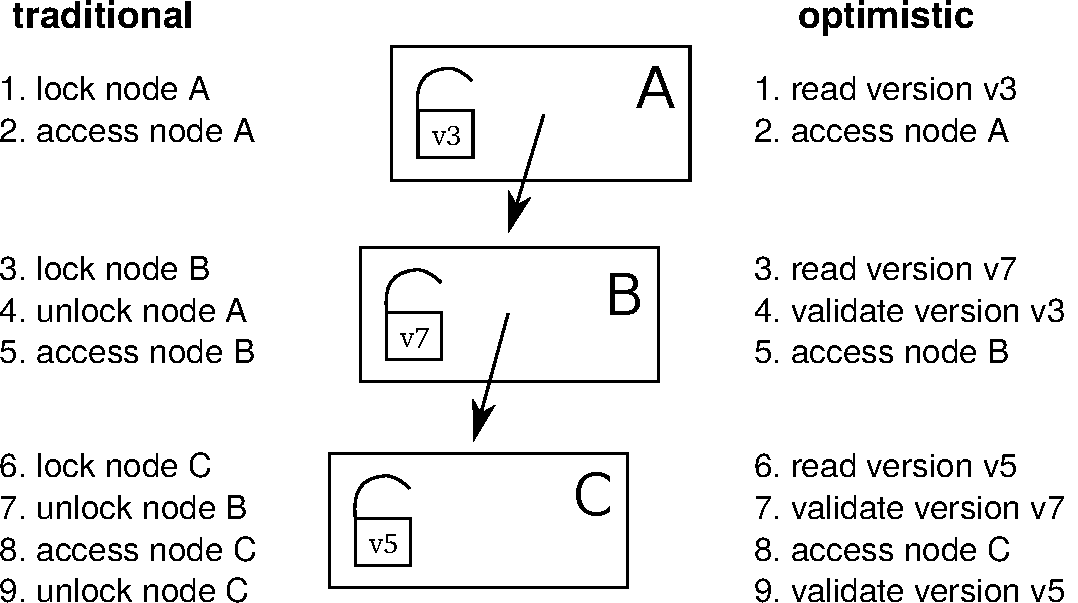
\includegraphics[width=0.65\linewidth]{olcall.pdf}
  \vspace{0.2cm}
  \caption{Comparison of a lookup operation in a 3-level tree using traditional lock coupling (left-hand side) vs.~optimistic lock coupling (right-hand side).}
  \label{fig:olc}
\end{figure}

The traditional and most common lock-based synchronization protocol for B-trees is lock coupling, which interleaves lock acquisitions while holding at most two locks at a time.
If, as we observed earlier, optimistic locks have similar semantics as traditional locks, it is natural to ask whether lock coupling can be combined with optimistic locks.
And indeed the answer is yes: One can almost mechanically translate traditional lock coupling code to optimistic lock coupling code.
This is illustrated in Figure~\ref{fig:olc}, which compares the traversal in a tree of height 3 using traditional and optimistic locks.
As the figure shows, the main difference is that locking is translated to reading the version and that unlocking becomes validation of the previously read version.
This simple change provides efficient lock-free tree traversal without the need to design a complex synchronization protocol.

It is important to emphasize the conceptual simplicity of OLC in comparison to data structures that use custom protocols like the Bw-tree~\cite{DBLP:conf/icde/LevandoskiLS13a}.
To implement lock-free access, the Bw-tree requires an indirection table, delta nodes, complex splitting and merging logic, retry logic, etc.
OLC, on the other hand, can directly be applied to B-trees mostly by adding the appropriate optimistic locking code and without modifying the node layout itself.
Therefore, OpenBw-Tree, an open source implementation of the Bw-tree, requires an order of magnitude more code than a B-tree based on OLC\footnote{Both implementations are available on GitHub: \url{https://github.com/wangziqi2016/index-microbench}}.
Given how difficult it is to develop, validate, and debug lock-free code, simplicity is obviously a major advantage.

\subsection{Correctness Aspects}

\begin{figure}
  % \centering
  %[basicstyle=\normalsize\ttfamily,showstringspaces=false,columns=fullflexible,breaklines=false,breakatwhitespace=true,numbers=none,numberstyle=\small,style=C,keepspaces=true]
\begin{lstlisting}[basicstyle=\ttfamily,language=C++,numbers=left,numberstyle=\small]
std::atomic<BTreeNode*> root;

// search for key in B+tree, returns payload in resultOut
bool lookup(Key key, Value& resultOut) {
   BTreeNode* node = root.load();
   uint64_t nodeVersion = node->readLockOrRestart();
   if (node != root.load()) // make sure the root is still the root
      restart();

   BTreeInner<Key>* parent = nullptr;
   uint64_t parentVersion = 0;

   while (node->isInner()) {
      auto inner = (BTreeInner*)node;

      // unlock parent and make current node the parent
      if (parent)
         parent->readUnlockOrRestart(parentVersion);
      parent = inner;
      parentVersion = nodeVersion;

      // search for next node
      node = inner->findChild(key);
      // validate 'inner' to ensure that 'node' pointer is valid
      inner->checkOrRestart(nodeVersion);
      // now it safe to dereference 'node' pointer (read its version)
      nodeVersion = node->readLockOrRestart();
   }

   // search in leaf and retrieve payload
   auto leaf = (BTreeLeaf*)node;
   bool success = leaf->findValue(key, resultOut);

   // unlock everything
   if (parent)
      parent->readUnlockOrRestart(parentVersion);
   node->readUnlockOrRestart(nodeVersion);

   return success;
}
\end{lstlisting}
  \vspace{0.2cm}
  \caption{B-tree lookup code using OLC. For simplicity, the restart logic is not shown.}
  \label{fig:lookup}
\end{figure}

So far, we have introduced the high-level ideas behind OLC and have stressed its similarity to traditional lock coupling.
Let us now discuss some cases where the close similarity between lock coupling and OLC breaks down.
To make this more concrete, we show the B-tree lookup code in Figure~\ref{fig:lookup}.
In the code, \texttt{readLockOrRestart} reads the lock version and \texttt{readUnlockOrRestart} validates that the read was correct.

One issue with OLC is that any pointer speculatively read from a node may point to invalid memory (if that node is modified concurrently).
Dereferencing such a pointer (e.g., to read its optimistic lock), may cause a segmentation fault or undefined behavior.
In the code shown in Figure~\ref{fig:lookup}, this problem is prevented by the extra check in line 25, which ensures that the read from the node containing the pointer was correct.
Without this additional validation, the code would in line 27 dereference the pointer speculatively read in line 23.
Note that the implementation of \texttt{checkOrRestart} is actually identical to \texttt{readUnlockOrRestart}.
We chose to give it a different name to highlight the fact that this extra check would not be necessary with read/write locks.

Another potential issue with optimistic locks is code that does not terminate.
Code that speculatively accesses a node, like an intra-node binary search, should be written in a way such that it always terminates---even in the presence of concurrent writes.
Otherwise, the validation code that detects the concurrent write will never run.
The binary search of a B-tree, for example, needs to be written in such a way that each comparison makes progress.
For some data structures that do not require loops in the traversal code (like ART) termination is trivially true.

\subsection{Implementation Details}

% implementation, efficiency
To implement an optimistic lock, one can combine the lock and the version counter into a single 64-bit\footnote{Even after subtracting one bit for the lock status, a back-of-the-envelope calculation can show that 63 bits are large enough to never overflow in practice.} word~\cite{artsync}.
A typical read operation will therefore merely consist of reading this version counter atomically.
In C++11 this can be implemented using the \texttt{std::atomic} type.

On x86, atomic reads are cheap because of x86's strong memory order guarantees.
No memory fences are required for sequentially-consistent loads, which are translated (by both GCC and clang) into standard \texttt{MOV} instructions.
Hence, the only effect of \texttt{std::atomic} for loads is preventing instruction re-ordering.
This makes version access and validation cheap.
Acquiring and releasing an optimistic lock in exclusive mode has comparable cost to a traditional lock:
A fairly expensive sequentially-consistent store is needed for acquiring a lock, while a standard \texttt{MOV} suffices for releasing it.
A simple sinlock-based implementation of optimistic locks can be found in the appendix of an earlier paper~\cite{artsync}.

OLC code must be able to handle restarts since validation or lock upgrade can fail due to concurrent writers.
Restarts can easily be implemented by wrapping the data structure operation in a loop (for simplicity not shown in Figure~\ref{fig:lookup}).
Such a loop also enables limiting the number of optimistic retry operations and falling back to pessimistic locking in cases of very heavy contention.
The ability to fall back to traditional locking is a major advantage of OLC in terms of robustness over lock-free approaches, which do not have this option.

In addition to the optimistic shared mode and the exclusive mode, optimistic locks also support a ``shared pessimistic'' mode, which physically acquires the lock in shared mode (allowing multiple concurrent readers but no writers).
This mode is useful for table (or range) scans that touch many tuples on a leaf page (which would otherwise easily abort).
Finally, let us mention that large range scans and table scans, should be broken up into several per-node traversals as is done in the LeanStore~\cite{leanstore} system.

Like all lock-free data structures, but unlike traditional locking and Hardware Transactional Memory~\cite{DBLP:conf/hpca/KarnagelDRLLSL14,DBLP:journals/pvldb/MakreshanskiLS15,htmtkde}, OLC requires care when deleting (and reusing) nodes.
The reason is that a deleting thread can never be sure that a node can be reclaimed because other threads might still be optimistically reading from that node.
Therefore, standard solutions like epoch-based reclamation~\cite{DBLP:conf/sosp/TuZKLM13}, hazard pointers~\cite{DBLP:journals/tpds/Michael04}, or optimized hazard pointers~\cite{DBLP:conf/spaa/BalmauGHZ16} need to be used.
These memory reclamation techniques are, however, largely orthogonal to the synchronization protocol itself.

%-lock-free is not a strong guarantee

\newpage
\section{Evaluation}\label{sec:evaluation}

Let us now experimentally evaluate the overhead and scalability of OLC.
For the experiments, we use an in-memory B+tree implemented in C++11 using templates, which is configured to use nodes of 4096 bytes, random 8 byte keys, and 8 byte payloads.
Based on this B-tree, we compare the following synchronization approaches:
\begin{itemize}
\item an OLC implementation\footnote{An almost identical OLC implementation is available on github: \url{https://github.com/wangziqi2016/index-microbench/tree/master/BTreeOLC}}
\item a variant based on traditional lock coupling and read/write locks
\item the unsynchronized B-tree, which obviously is only correct for read-only workloads but allows measuring the overhead of synchronization
\end{itemize}
Note that earlier work has compared the OLC implementation with a Bw-tree implementation~\cite{buzzword} and other state-of-the-art in-memory index structures.

We use a Haswell EP system with an Intel Xeon E5-2687W v3 CPU, which has 10 cores (20 ``Hyper-Threads'') and 25~MB of L3 cache.
The system is running Ubuntu 18.10 and we use GCC 8.2.0 to compile our code.
The CPU counters are obtained using the Linux perf API\footnote{We use the following convenience wrapper: \url{https://github.com/viktorleis/perfevent}}.

\begin{table}
  \caption{Performance and CPU counters for lookup and insert operations in a B-tree with 100M keys. We perform 100M operations and normalize the CPU counters by that number.}
  \label{tab:overhead}
  \centering
  \begin{tabular}{lrrrrrrr}\toprule
                    &         &        &        & instruc-  & L1     & L3     & branch \\
                    & threads & M op/s & cycles & tions & misses & misses & misses \\\midrule
lookup (no sync.)   & 1       & 1.72   & 2028   & 283     & 39.1   & 14.9   & 16.1   \\
lookup (OLC)        & 1       & 1.65   & 2107   & 370     & 43.9   & 15.1   & 16.7   \\
lookup (lock coup.) & 1       & 1.72   & 2078   & 365     & 42.3   & 16.9   & 15.7   \\\midrule
insert (no sync.)   & 1       & 1.51   & 2286   & 530     & 59.8   & 31.1   & 17.3   \\
insert (OLC)        & 1       & 1.50   & 2303   & 629     & 61.2   & 31.1   & 16.5   \\
insert (lock coup.) & 1       & 1.41   & 2473   & 644     & 61.0   & 31.0   & 17.2   \\\midrule
lookup (no sync.)   & 10      & 15.48  & 2058   & 283     & 38.6   & 15.5   & 16.0   \\
lookup (OLC)        & 10      & 14.60  & 2187   & 370     & 43.8   & 15.8   & 16.8   \\
lookup (lock coup.) & 10      & 5.71   & 5591   & 379     & 54.2   & 17.0   & 14.8   \\\midrule
insert (no sync.)   & 10      & -      & -      & -       & -      & -      & -      \\
insert (OLC)        & 10      & 10.46  & 2940   & 656     & 62.0   & 32.5   & 16.8   \\
insert (lock coup.) & 10      & 7.55   & 4161   & 667     & 75.0   & 28.6   & 16.2   \\
    \bottomrule
\end{tabular}
\end{table}

Table~\ref{tab:overhead} compares the performance and CPU counters for lookup and insert operations in a B-tree with 100M keys.
With {\em single-threaded} execution, we observe that all three approaches have very similar performance.
Adding traditional or optimistic locks to unsynchronized B-tree code results in up to 30\% of additional instructions without affecting single-threaded performance much.

\begin{figure}
  \centering
  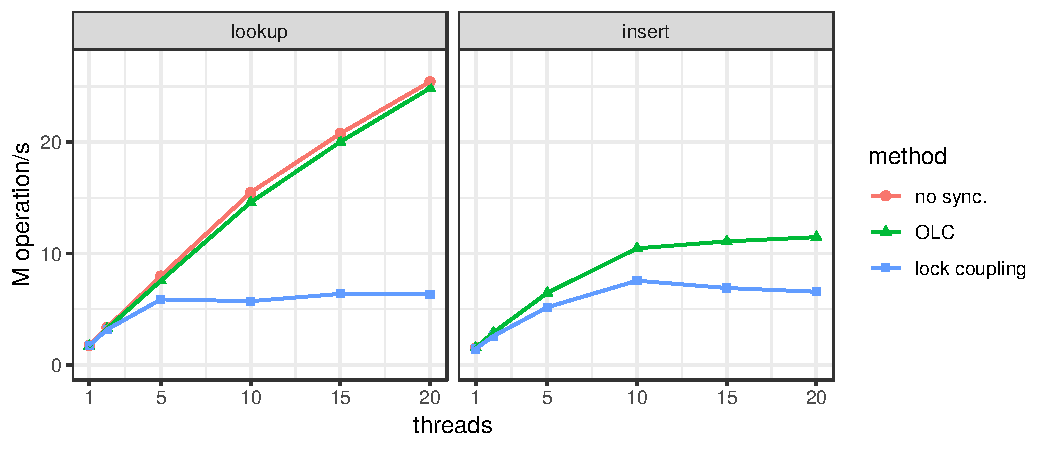
\includegraphics[width=\linewidth]{scale.pdf}
  \vspace{0.2cm}
  \caption{Scalability on 10-core system for B-tree operations (100M values).}
  \label{fig:scale}
\end{figure}

As Figure~\ref{fig:scale} shows, the results change dramatically once we use multiple threads.
For lookup, the scalability of OLC is near-linear up to 20 threads, even though the system has only 10 ``real cores''.
The OLC scalability for insert is also respectable (though not quite as linear because multi-threaded insertion approaches the memory bandwidth of our processor).
The figure also shows that the results of traditional lock coupling with read/write locks are significantly worse than OLC.
With 20 threads, lookup with OLC is 3.9$\times$ faster than traditional lock coupling.

\section{Summary}\label{sec:conc}

Optimistic Lock Coupling (OLC) is an effective synchronization method that combines the simplicity of traditional lock coupling with the superior scalability of lock-free approaches.
OLC is widely applicable and has already been successfully used to synchronize several data structures, including B-trees, binary search trees, and different trie variants.
These features make it highly attractive for modern database systems as well as performance-critical systems software in general.

\begin{thebibliography}{10}

\bibitem{DBLP:conf/spaa/BalmauGHZ16}
O.~Balmau, R.~Guerraoui, M.~Herlihy, and I.~Zablotchi.
\newblock Fast and robust memory reclamation for concurrent data structures.
\newblock In {\em SPAA}, 2016.

\bibitem{DBLP:journals/acta/BayerS77}
R.~Bayer and M.~Schkolnick.
\newblock Concurrency of operations on {B}-trees.
\newblock {\em Acta Informatica}, 9, 1977.

\bibitem{hot}
R.~Binna, E.~Zangerle, M.~Pichl, G.~Specht, and V.~Leis.
\newblock {HOT}: A height optimized trie index for main-memory database
  systems.
\newblock In {\em SIGMOD}, 2018.

\bibitem{DBLP:conf/ppopp/BronsonCCO10}
N.~G. Bronson, J.~Casper, H.~Chafi, and K.~Olukotun.
\newblock A practical concurrent binary search tree.
\newblock In {\em PPOPP}, 2010.

\bibitem{DBLP:conf/vldb/ChaHKK01}
S.~K. Cha, S.~Hwang, K.~Kim, and K.~Kwon.
\newblock Cache-conscious concurrency control of main-memory indexes on
  shared-memory multiprocessor systems.
\newblock In {\em VLDB}, 2001.

\bibitem{intel}
I.~Cutress.
\newblock {Intel} goes for 48-cores: {Cascade-AP} with multi-chip package
  coming soon.
\newblock
  \url{https://www.anandtech.com/show/13535/intel-goes-for-48cores-cascade-ap},
  2018 (accessed January, 2019).

\bibitem{DBLP:conf/cidr/FaleiroA17}
J.~M. Faleiro and D.~J. Abadi.
\newblock Latch-free synchronization in database systems: Silver bullet or
  fool's gold?
\newblock In {\em CIDR}, 2017.

\bibitem{DBLP:journals/ftdb/Graefe11}
G.~Graefe.
\newblock Modern {B}-tree techniques.
\newblock {\em Foundations and Trends in Databases}, 3(4), 2011.

\bibitem{DBLP:conf/hpca/KarnagelDRLLSL14}
T.~Karnagel, R.~Dementiev, R.~Rajwar, K.~Lai, T.~Legler, B.~Schlegel, and
  W.~Lehner.
\newblock Improving in-memory database index performance with
  {Intel}\({}^{\mbox{{\textregistered}}}\) transactional synchronization
  extensions.
\newblock In {\em HPCA}, 2014.

\bibitem{DBLP:journals/tods/LehmanY81}
P.~L. Lehman and S.~B. Yao.
\newblock Efficient locking for concurrent operations on {B}-trees.
\newblock {\em {ACM} Trans. Database Syst.}, 6(4), 1981.

\bibitem{leanstore}
V.~Leis, M.~Haubenschild, A.~Kemper, and T.~Neumann.
\newblock Leanstore: In-memory data management beyond main memory.
\newblock In {\em ICDE}, 2018.

\bibitem{art}
V.~Leis, A.~Kemper, and T.~Neumann.
\newblock The adaptive radix tree: {ARTful} indexing for main-memory databases.
\newblock In {\em ICDE}, 2013.

\bibitem{htmtkde}
V.~Leis, A.~Kemper, and T.~Neumann.
\newblock Scaling {HTM}-supported database transactions to many cores.
\newblock {\em {IEEE} Trans. Knowl. Data Eng.}, 28(2), 2016.

\bibitem{artsync}
V.~Leis, F.~Scheibner, A.~Kemper, and T.~Neumann.
\newblock The {ART} of practical synchronization.
\newblock In {\em DaMoN}, 2016.

\bibitem{DBLP:conf/icde/LevandoskiLS13a}
J.~J. Levandoski, D.~B. Lomet, and S.~Sengupta.
\newblock The {Bw}-tree: A {B}-tree for new hardware platforms.
\newblock In {\em ICDE}, 2013.

\bibitem{DBLP:journals/pvldb/MakreshanskiLS15}
D.~Makreshanski, J.~J. Levandoski, and R.~Stutsman.
\newblock To lock, swap, or elide: On the interplay of hardware transactional
  memory and lock-free indexing.
\newblock {\em {PVLDB}}, 8(11), 2015.

\bibitem{DBLP:dblp_conf/eurosys/MaoKM12}
Y.~Mao, E.~Kohler, and R.~T. Morris.
\newblock Cache craftiness for fast multicore key-value storage.
\newblock In {\em EuroSys}, 2012.

\bibitem{DBLP:journals/tpds/Michael04}
M.~M. Michael.
\newblock Hazard pointers: Safe memory reclamation for lock-free objects.
\newblock {\em {IEEE} Trans. Parallel Distrib. Syst.}, 15(6), 2004.

\bibitem{DBLP:journals/jacm/ShalevS06}
O.~Shalev and N.~Shavit.
\newblock Split-ordered lists: Lock-free extensible hash tables.
\newblock {\em J. {ACM}}, 53(3), 2006.

\bibitem{amd}
A.~Shilov.
\newblock {AMD} previews {EPYC} ‘{Rome}’ processor: Up to 64 {Zen} 2 cores.
\newblock
  \url{https://www.anandtech.com/show/13561/amd-previews-epyc-rome-processor-up-to-64-zen-2-cores},
  2018 (accessed January, 2019).

\bibitem{DBLP:conf/sosp/TuZKLM13}
S.~Tu, W.~Zheng, E.~Kohler, B.~Liskov, and S.~Madden.
\newblock Speedy transactions in multicore in-memory databases.
\newblock In {\em SOSP}, 2013.

\bibitem{buzzword}
Z.~Wang, A.~Pavlo, H.~Lim, V.~Leis, H.~Zhang, M.~Kaminsky, and D.~Andersen.
\newblock Building a {Bw}-tree takes more than just buzz words.
\newblock In {\em SIGMOD}, 2018.

\end{thebibliography}


%\bibliographystyle{abbrv}
%\bibliography{main}

\end{document}

\end{article}
\end{articlesection}

% put the news items below- there can be multiple news sections
% each with its own title
% news will usually have an author as well as a title,
% e.g. TCDE elections
% news articles are in the same format as letters
% typically, news articles will be stored in a directory called "news"


% \begin{newssection}{Obituary}
% \begin{news}{Obituary for Professor Gio Wiederhold}
% {Kyu-Young Whang and Marianne Winslett}{Distinguished Professor Emeritus, KAIST\\ Research Professor Emerita, UIUC\\ together with Gio’s other former students}
% \documentclass[11pt]{article} 

\usepackage{deauthor,times,graphicx}
%\usepackage{url}
\usepackage{hyperref}

\begin{document}
%Obituary for Professor Gio Wiederhold
%                                                                  December 26, 2022                                                                         
Professor Gio Wiederhold passed away in the early hours of December 26, 2022, aged 86, just 10 weeks after an unexpected diagnosis of stage 4 liver cancer. Gio died at home, surrounded by his family members who had gathered for Christmas, including his wife of 56 years, Voy Wiederhold, and his sons John and Randy.  


Gio was a great scholar, educator, and mentor. His influence on the database field is immense. As a pioneer in the database field, he wrote the influential 1977 textbook Database Design, one of the first in the field and adopted around the world. In his DARPA-supported Knowledge-Base Management Systems project in the early 1980s, Gio pioneered the concept of integrating databases and AI, a topic that is now enjoying a revival. Beginning in the 1970s, Gio also pursued the application of databases to medical informatics, another area just now entering the mainstream. In 1992, Gio introduced the notion of mediators (IEEE Computer) as a way of intelligently integrating information from large-scale heterogeneous sources such as databases, file systems, and repositories, a seminal idea for the nascent field of information integration. Gio continued to innovate after retirement from Stanford, most notably in establishing an approach for valuing software and the intellectual property of multinational firms.


Gio advised 36 PhD students at Stanford. Today, Gio’s academic descendants can be found in companies and universities all over the world, including early students Hector Garcia-Molina (the late Stanford professor), David Shaw (DE Shaw founder), Ramez Elmasri (the late textbook author and UT Arlington professor), Kyu-Young Whang (KAIST professor and Naver founder’s advisor), and Marianne Winslett (UIUC professor). Gio’s many subsequent students continue to lead the database field today. 


An influential mentor, Gio always emphasized the practical aspects of research, encouraging people to develop both theoretical and engineering approaches to solve real-world problems. This outlook stemmed from his many years of experience in computing practice before he joined the Stanford University faculty.


Gio’s service to the professional community includes serving as the third Editor-in-Chief of ACM Transactions on Databases during 1985-1995, during which time he significantly contributed to making the new journal a top one in the field. Together with five colleagues, Gio co-founded the IEEE International Conference on Data Engineering in 1984. Perhaps the first venue to use the term data engineering, the conference was unique in focusing on engineering aspects of database research; today it stands as one of the three top-tier conferences in database research. Gio also served as the conference’s program committee chair, co-chair, and general chair in its early years. During 1991-1994, Gio served as the program manager for DARPA’s Knowledge-based Systems program, which collaborated with NSF to fund innovative new research related to information integration and digital libraries — including the project that led to the creation of Google.


In recognition of his many contributions, Gio received the IEEE Technical Community on Data Engineering’s Service Award in 2016. He was also a Fellow of the ACM, the IEEE, and the American College of Medical Informatics.




The many accomplishments and contributions listed above do not capture the full extent of Gio’s impact and influence on our community, nor his diligence and persistence. As Gio’s former students, we dearly miss him for his warm heart towards his students, colleagues, and friends, and above all, his love and kindness for everyone he knew. We are deeply saddened by Gio’s unexpected death and send our sincerest condolences to his surviving family and friends.  




%-- Kyu-Young Whang, Distinguished Professor Emeritus, KAIST and Marianne Winslett, Research Professor Emerita, University of Illinois at Urbana-Champaign, together with Gio’s other former students
\end{document}

% \end{news}

% \newpage
% \end{newssection}


\begin{callsection}

%  This section will be empty for your version
%
%  Calls for papers section.  Use the callsection environment.
%  Each call for papers is contained in an call environment, where the single
%  required options to \begin{call} is the name of the conference.
% typically calls are stored in a "calls" directory
%
%\begin{call}{name of conference}
%\centerline{\includegraphics[width=\textwidth, bb= 0 0 590 760]{calls/conference-name.pdf}}
%\end{call}
%\begin{call}{ICDE 2019 Conference}
%\centerline{
\includegraphics[width=\textwidth, bb= 0 0 610 790] {../Dec-2018/calls/icde19.pdf}}
%\centerline{
\includegraphics[width=\textwidth, bb= 0 0 590 760] {calls/icde19.pdf}}
%\end{call}
\begin{call}{TCDE Membership Form}
%\centerline{\includegraphics[width=\textwidth, bb= 0 0 610 790]
%\centerline{
\includegraphics[width=\textwidth, bb= 0 0 590 760] {../Dec-2018/calls/tcde.pdf}}
\centerline{
\includegraphics[width=\textwidth, bb= 0 0 590 760] {./calls/tcde.pdf}}
\end{call}

\end{callsection}

\end{bulletin}
\end{document}
